\documentclass[]{article}



\usepackage{graphicx,forloop,caption,subcaption,float,hyperref,arrayjob,listings,color,booktabs,mathtools}
\usepackage{pdfpages}
\usepackage[margin=1.2in]{geometry}
\usepackage{amsmath}
\usepackage{multirow}
%vhdl code
\definecolor{dkgreen}{rgb}{0,0.6,0}
\definecolor{gray}{rgb}{0.5,0.5,0.5}
\definecolor{mauve}{rgb}{0.58,0,0.82}

\DeclareMathOperator*{\argmin}{\arg\!\min}


\lstset{frame=tb,
  language=VHDL,
  aboveskip=3mm,
  belowskip=3mm,
  showstringspaces=false,
  columns=flexible,
  basicstyle={\small\ttfamily},
  numbers=none,
  numberstyle=\tiny\color{gray},
  keywordstyle=\color{blue},
  commentstyle=\color{dkgreen},
  stringstyle=\color{mauve},
  breaklines=true,
  breakatwhitespace=true
  tabsize=3
}

%matlab code
\lstset{frame=tb,
  language=Matlab,
  aboveskip=3mm,
  belowskip=3mm,
  showstringspaces=false,
  columns=flexible,
  basicstyle={\small\ttfamily},
  numbers=none,
  numberstyle=\tiny\color{gray},
  keywordstyle=\color{blue},
  commentstyle=\color{dkgreen},
  stringstyle=\color{mauve},
  breaklines=true,
  breakatwhitespace=true
  tabsize=3
}


% Title Page
\title{UCLA\\EE230B\\Digital Communication Design Project\\Step 2 Report}
\author{Alican Salor 404271991 \\  \href{mailto:alicansalor@ucla.edu}{alicansalor@ucla.edu} \\ \\
Darren Reis 804359840 \\
\href{mailto:darrer.r.reis@gmail.com}{darren.r.reis@gmail.com} }


\begin{document}
\maketitle

\newpage
\tableofcontents

\newpage


\section{System Setup}
\label{sec:setup}
The system is as shown in Figure below:

\begin{figure}[H]
\centering
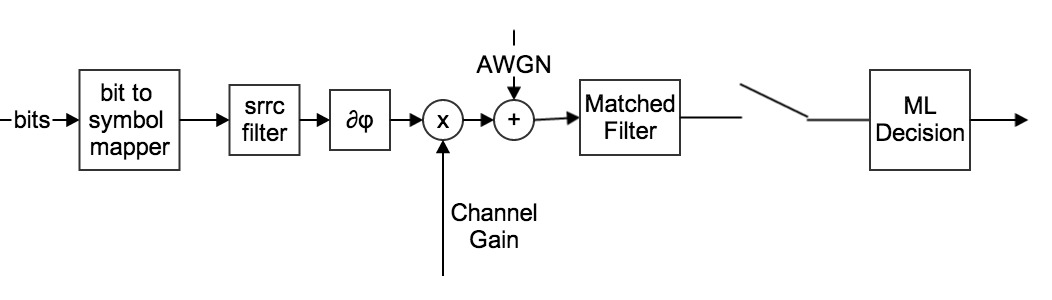
\includegraphics[width=\textwidth]{step2.jpg}
\caption{Diagram of the setup used in step 2 of the project}
\end{figure}

In addition to the modeling blocks used previously, non coherent error was included in the model.  The $\delta\phi$ block represents a block that introduces phase or frequency offset on the carrier.  The effect of this is to rotate and blur the constellations and the SNR plots [Section~\ref{sec:qam16_phaseConst}].

The new block was modeled by two different functions.  For Phase offset, the signal was subjected to a constant phase bias, as described in Appendix~\ref{app:phase_offset}.  Similarly, the Frequency offsets were handled by introducing a first order phase term.  Recall, phase is related to frequency by $f(t) = \frac{1}{2 \pi} \phi^\prime(t)$.  Appendix~\ref{app:freq_offset} shows how this was implemented in the simulations.

With the new design worked out, the system was put through a similar set of tests on the four modulation schemes: BPSK, QPSK, 16-QAM, 64-QAM.  Each was subjected to phase offsets from $5\deg$ to $45\deg$ for a range of SNR levels.  Similarly, the modulated signals faced frequency offsets from 10 mHz to 10 Hz.  The system performance was determined by comparing a theoretical error rate to experimental bit error rate.  
\section{Derivation of Errors}
\label{sec:errors}
The following are theoretical formulae for bit error rate under phase error \cite{howald}.

\begin{equation}
P_b^{\left( QPSK \right)} = \frac{1}{2}\left[Q\left(\sqrt{\frac{4E_b}{N_0}}sin\left(\frac{\pi}{4}+\theta\right)\right) + Q\left(\sqrt{\frac{4E_b}{N_0}}sin\left(\frac{3\pi}{4}+\theta\right)\right)\right]
\end{equation}

\section{Step 2 Phase Offset Results}
\label{sec:results_po}
In the following sections, the probability of bit error versus the signal to noise ratio is shown on scatter plots for BPSK, QPSK, 16-QAM and 64-QAM constellations .

\subsection{Probability of Error vs SNR plots for constellations with Phase Offset}
In the sections given below considering BPSK, QPSK, 16-QAM and 64-QAM constellations the following  are plotted using the MATLAB functions given in the appendix:
\begin{itemize}
\item Theoretical Bit Error Rate/Symbol Error Rate curve as a function of the symbol SNR
\item The theoretical Bit Error Rate/Symbol Error Rate curve as a function of $E_b/N_o$
\item The Bit Error Rate/Symbol Error Rate curve from the simulation as a function of the received signal's SNR
\end{itemize}

\subsubsection{BPSK with Phase Offset}
\label{sec:bpsk_phase}
\begin{figure}[H]
\centering
\hspace*{-2cm}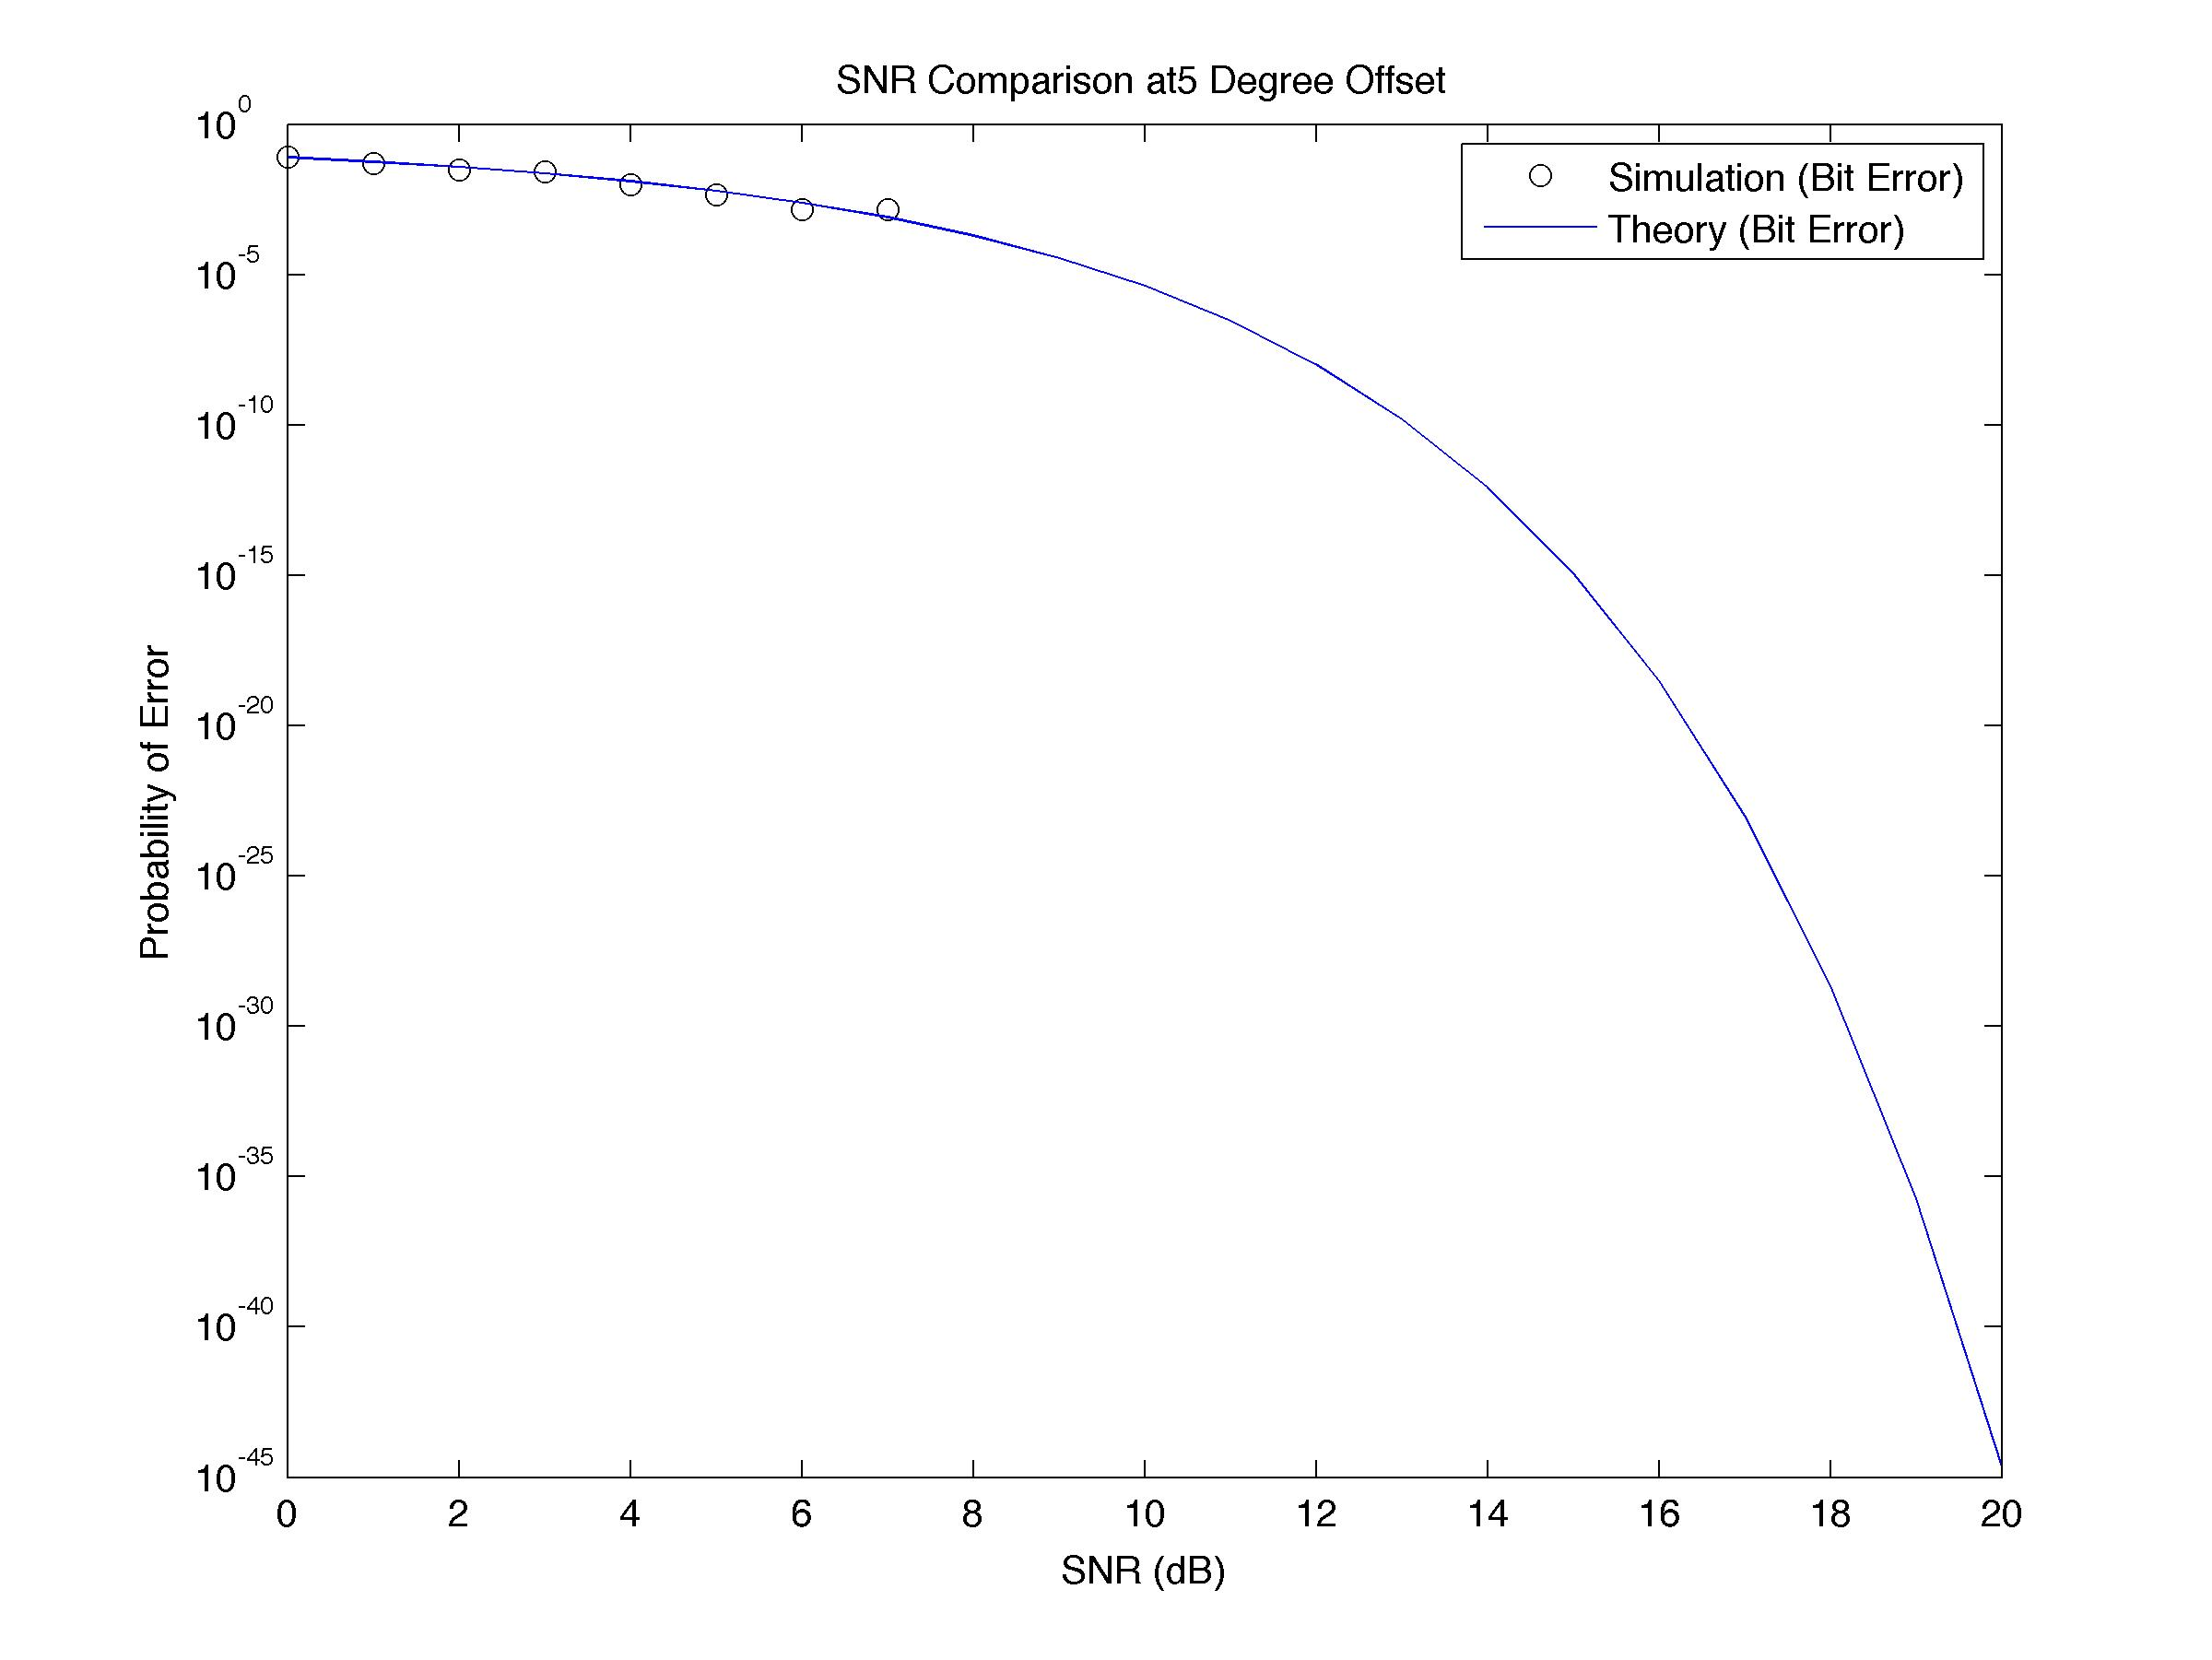
\includegraphics[width=1.3\textwidth]{bpSNRpo1.jpg}
\caption{BPSK Theoretical and Experimental error rates versus different SNR levels at a phase offset of 5 degrees }
\end{figure}

\begin{figure}[H]
\centering
\hspace*{-2cm}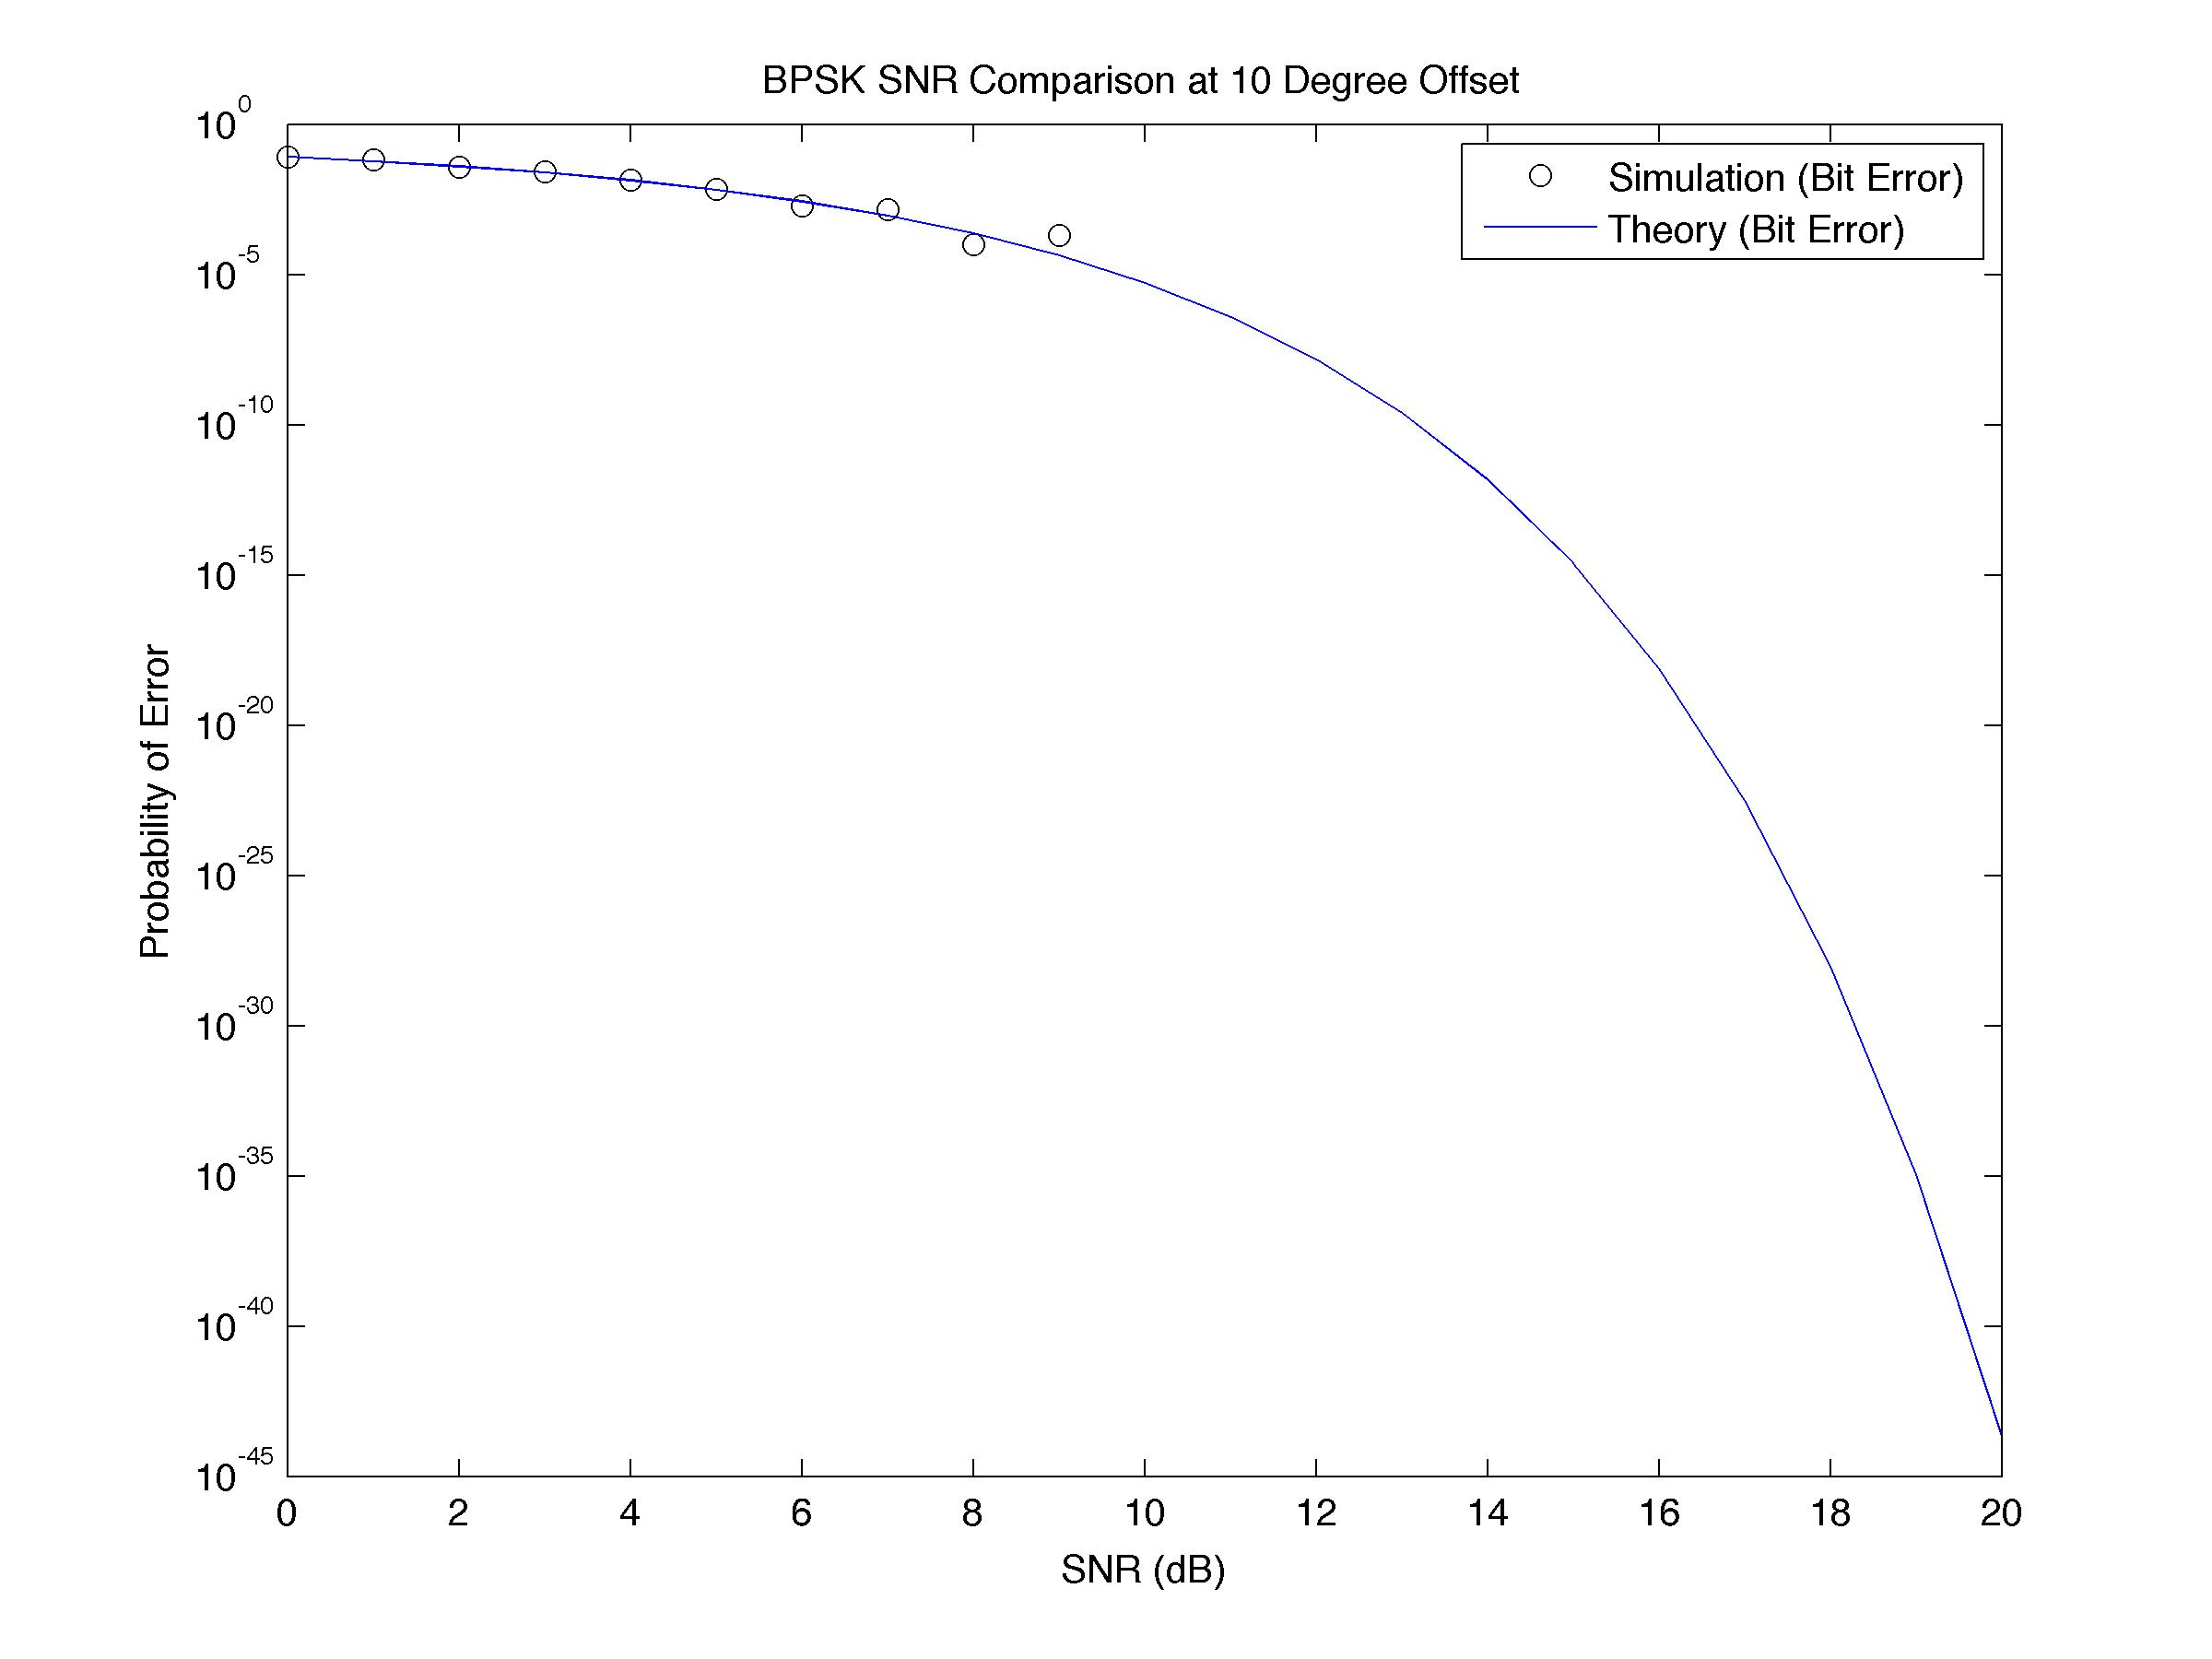
\includegraphics[width=1.3\textwidth]{bpSNRpo2.jpg}
\caption{BPSK Theoretical and Experimental error rates versus different SNR levels at a phase offset of 10 degrees }
\end{figure}


\begin{figure}[H]
\centering
\hspace*{-2cm}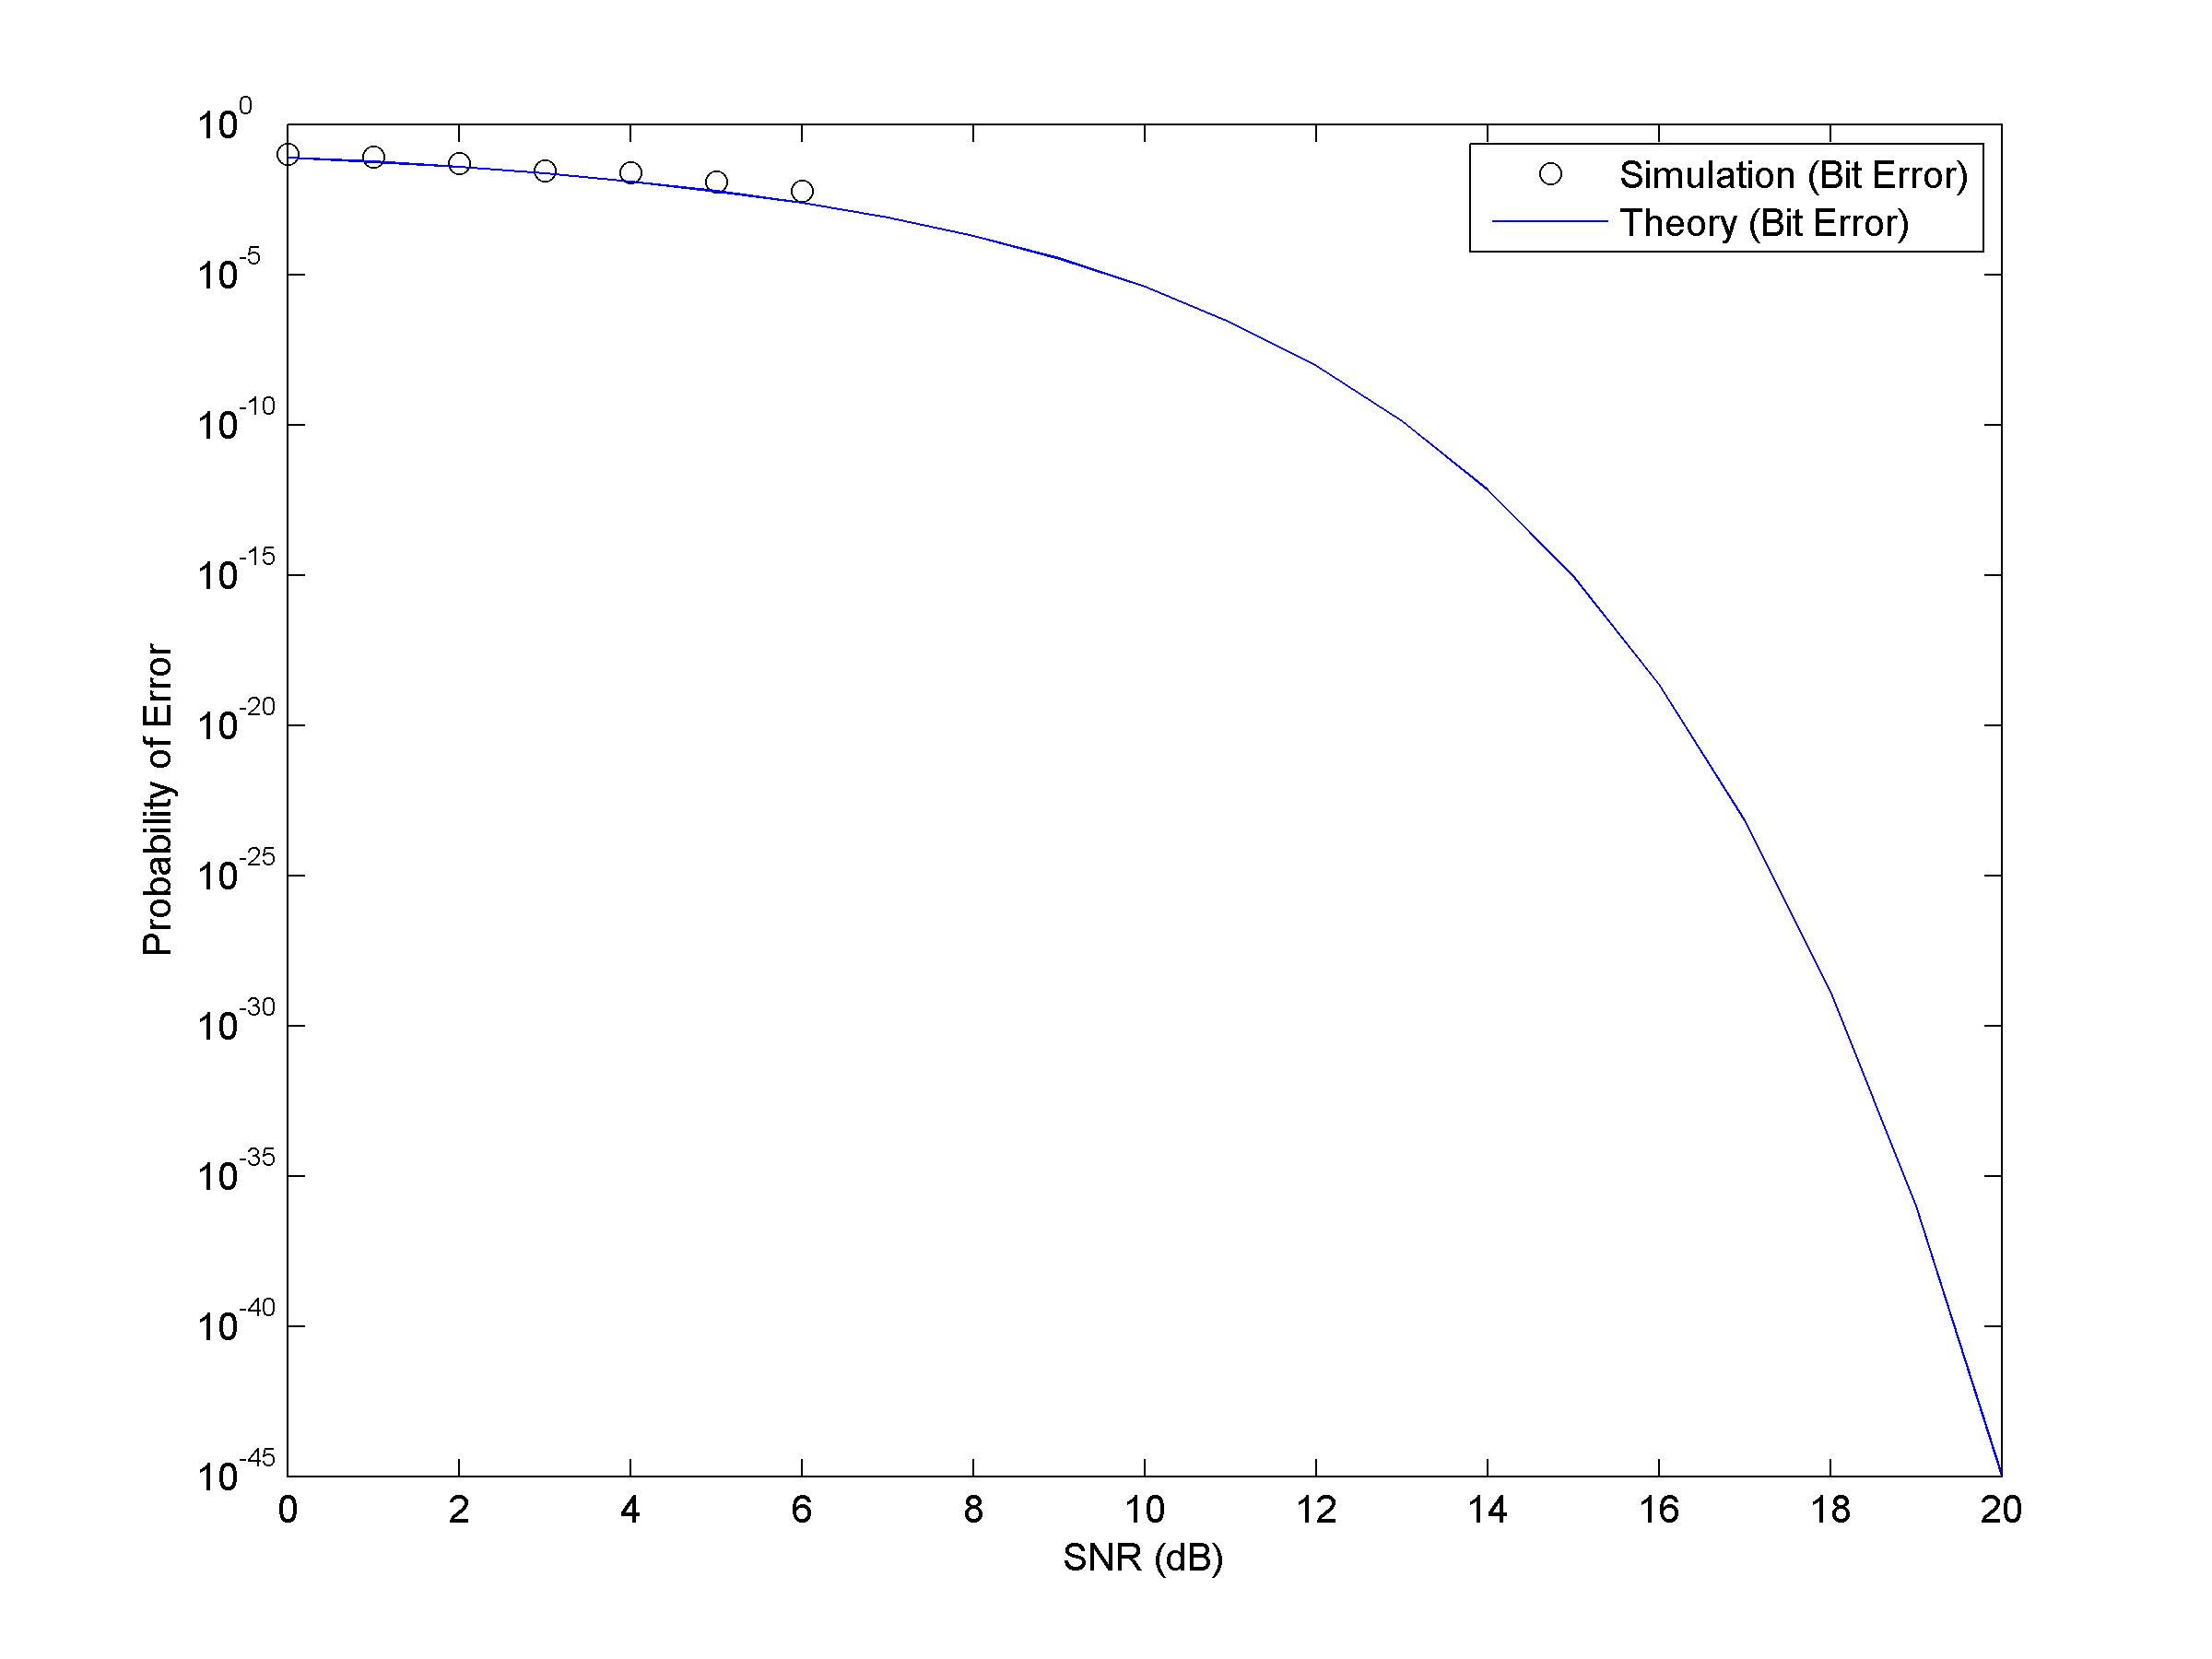
\includegraphics[width=1.3\textwidth]{bpSNRpo3.jpg}
\caption{BPSK Theoretical and Experimental error rates versus different SNR levels at a phase offset of 20 degrees }
\end{figure}

\begin{figure}[H]
\centering
\hspace*{-2cm}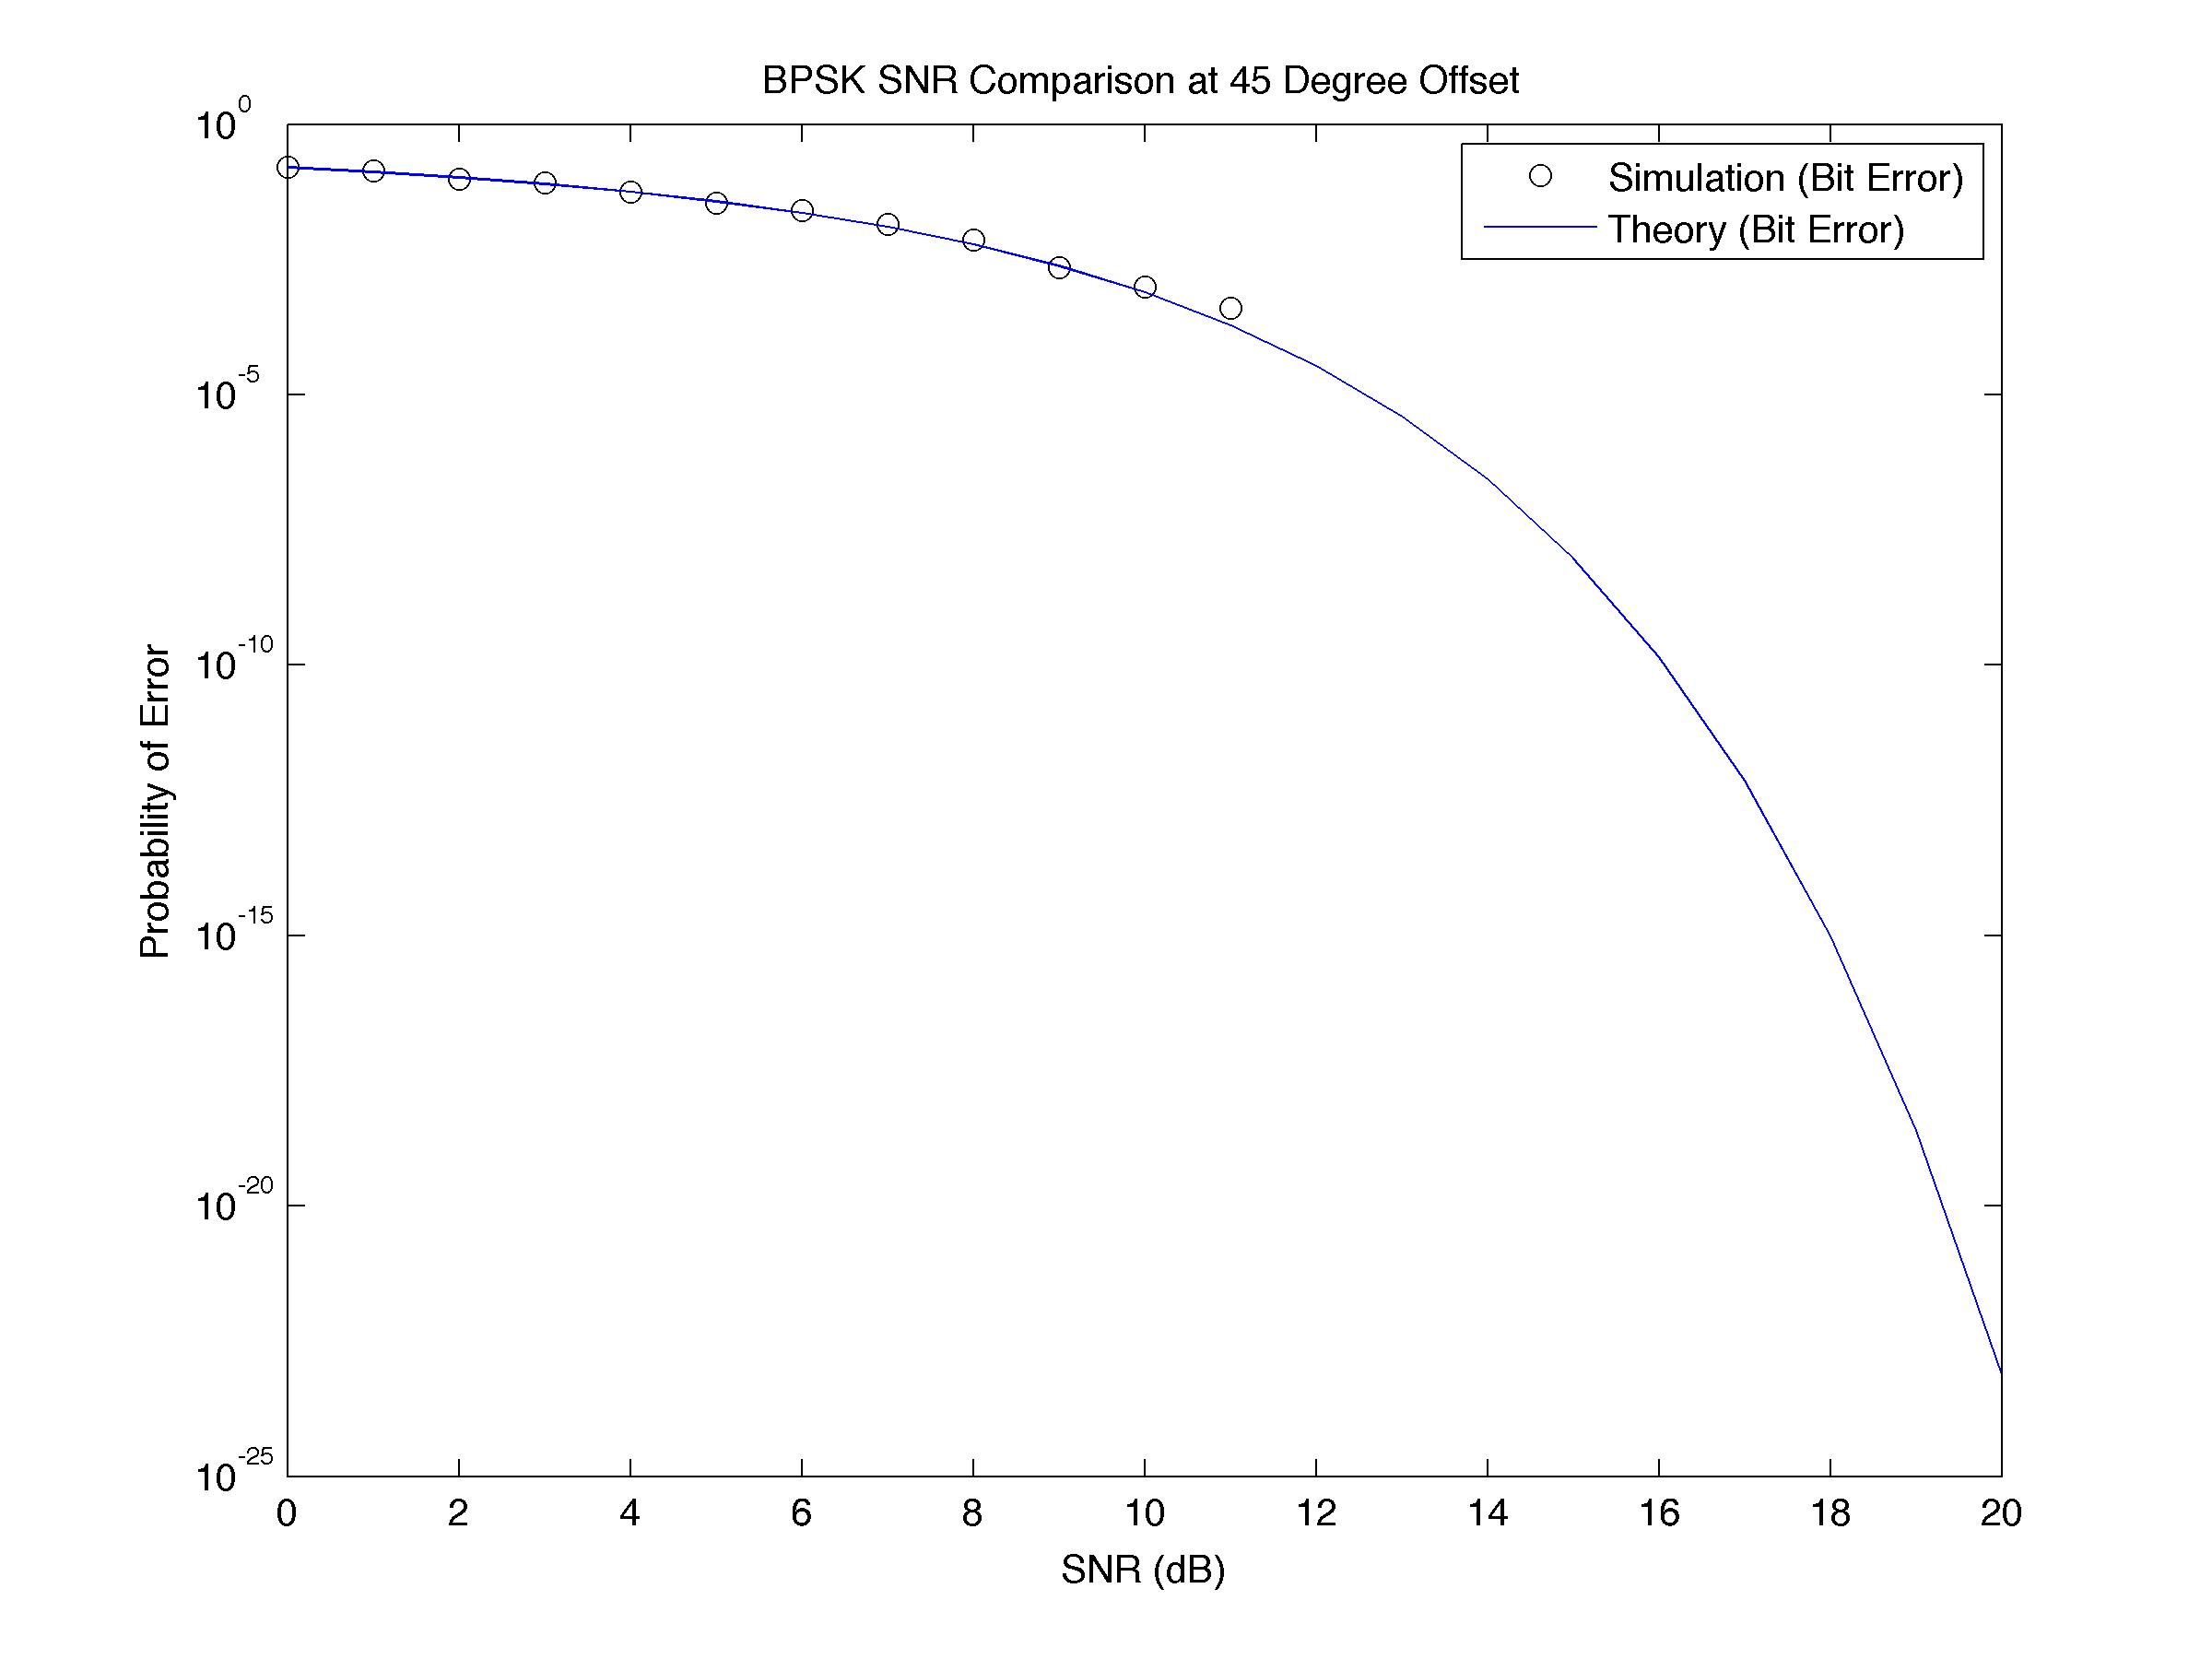
\includegraphics[width=1.3\textwidth]{bpSNRpo4.jpg}
\caption{BPSK Theoretical and Experimental error rates versus different SNR levels at a phase offset of 45 degrees }
\end{figure}


\subsubsection{QPSK with Phase Offset}
\label{sec:qpsk_phase}
\begin{figure}[H]
\centering
\hspace*{-2cm}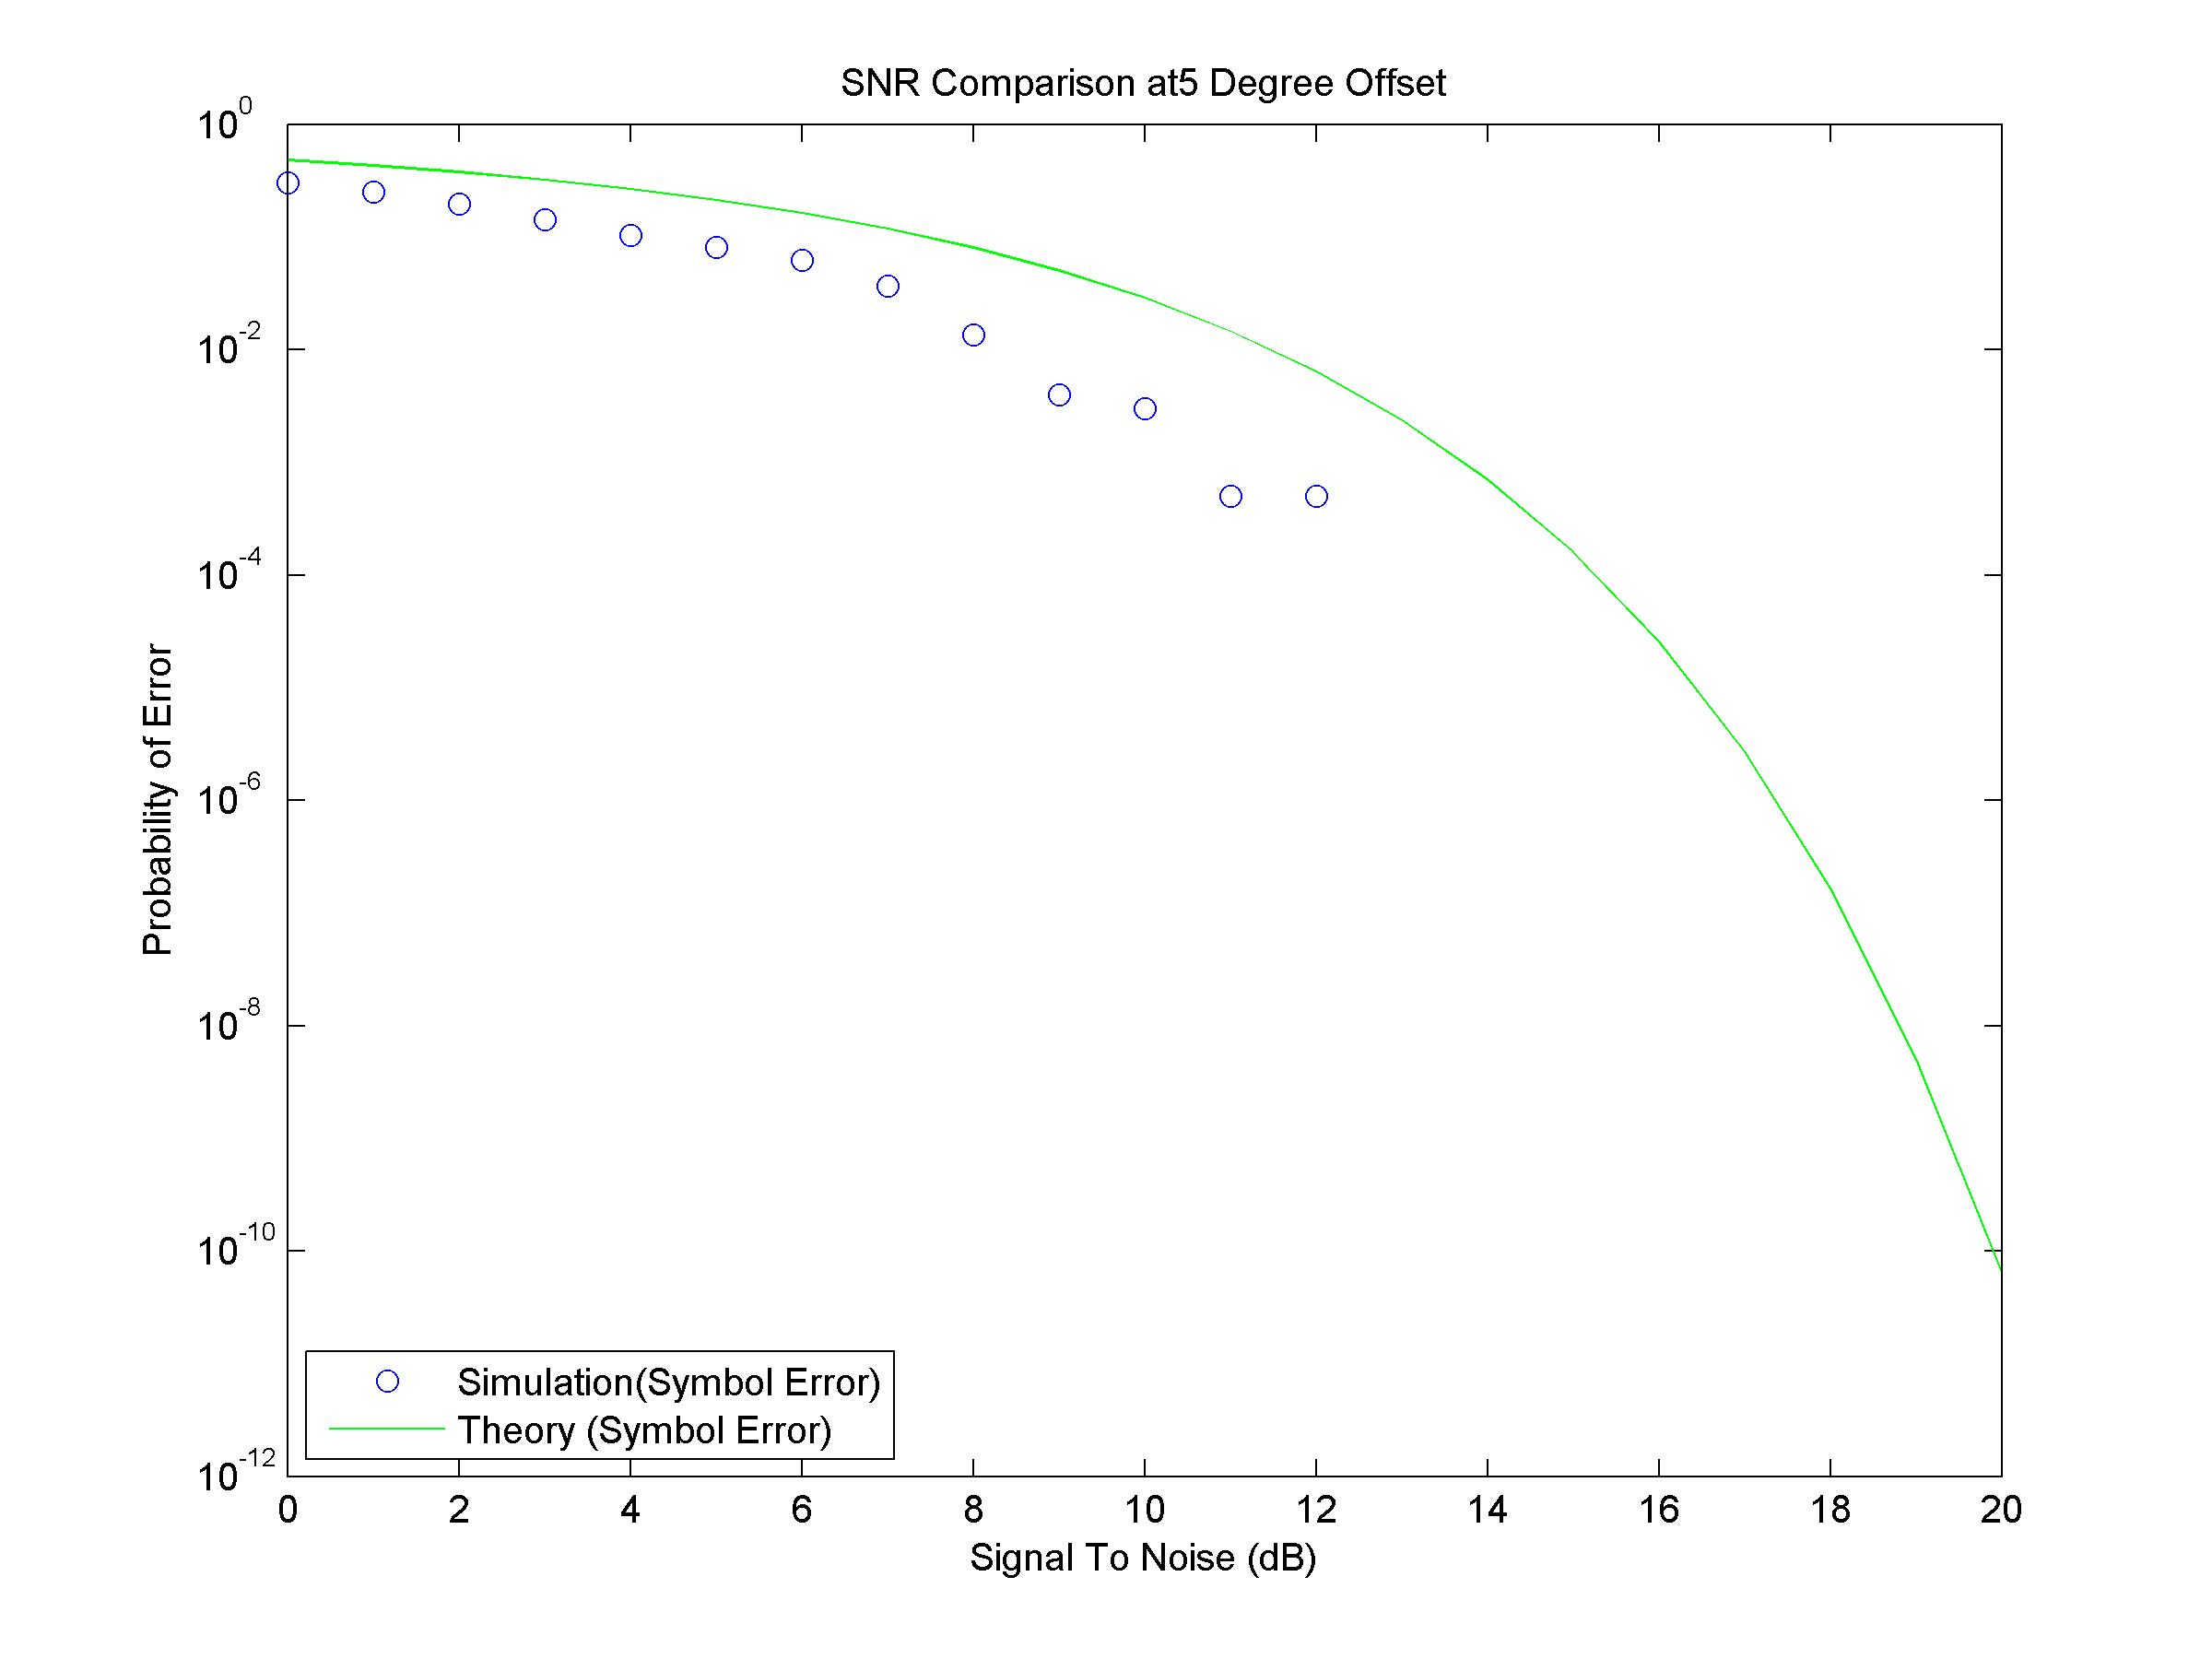
\includegraphics[width=1.3\textwidth]{qpSNRpo1.jpg}
\caption{QPSK Theoretical and Experimental error rates versus different SNR levels at a phase offset of 5 degrees }
\end{figure}

\begin{figure}[H]
\centering
\hspace*{-2cm}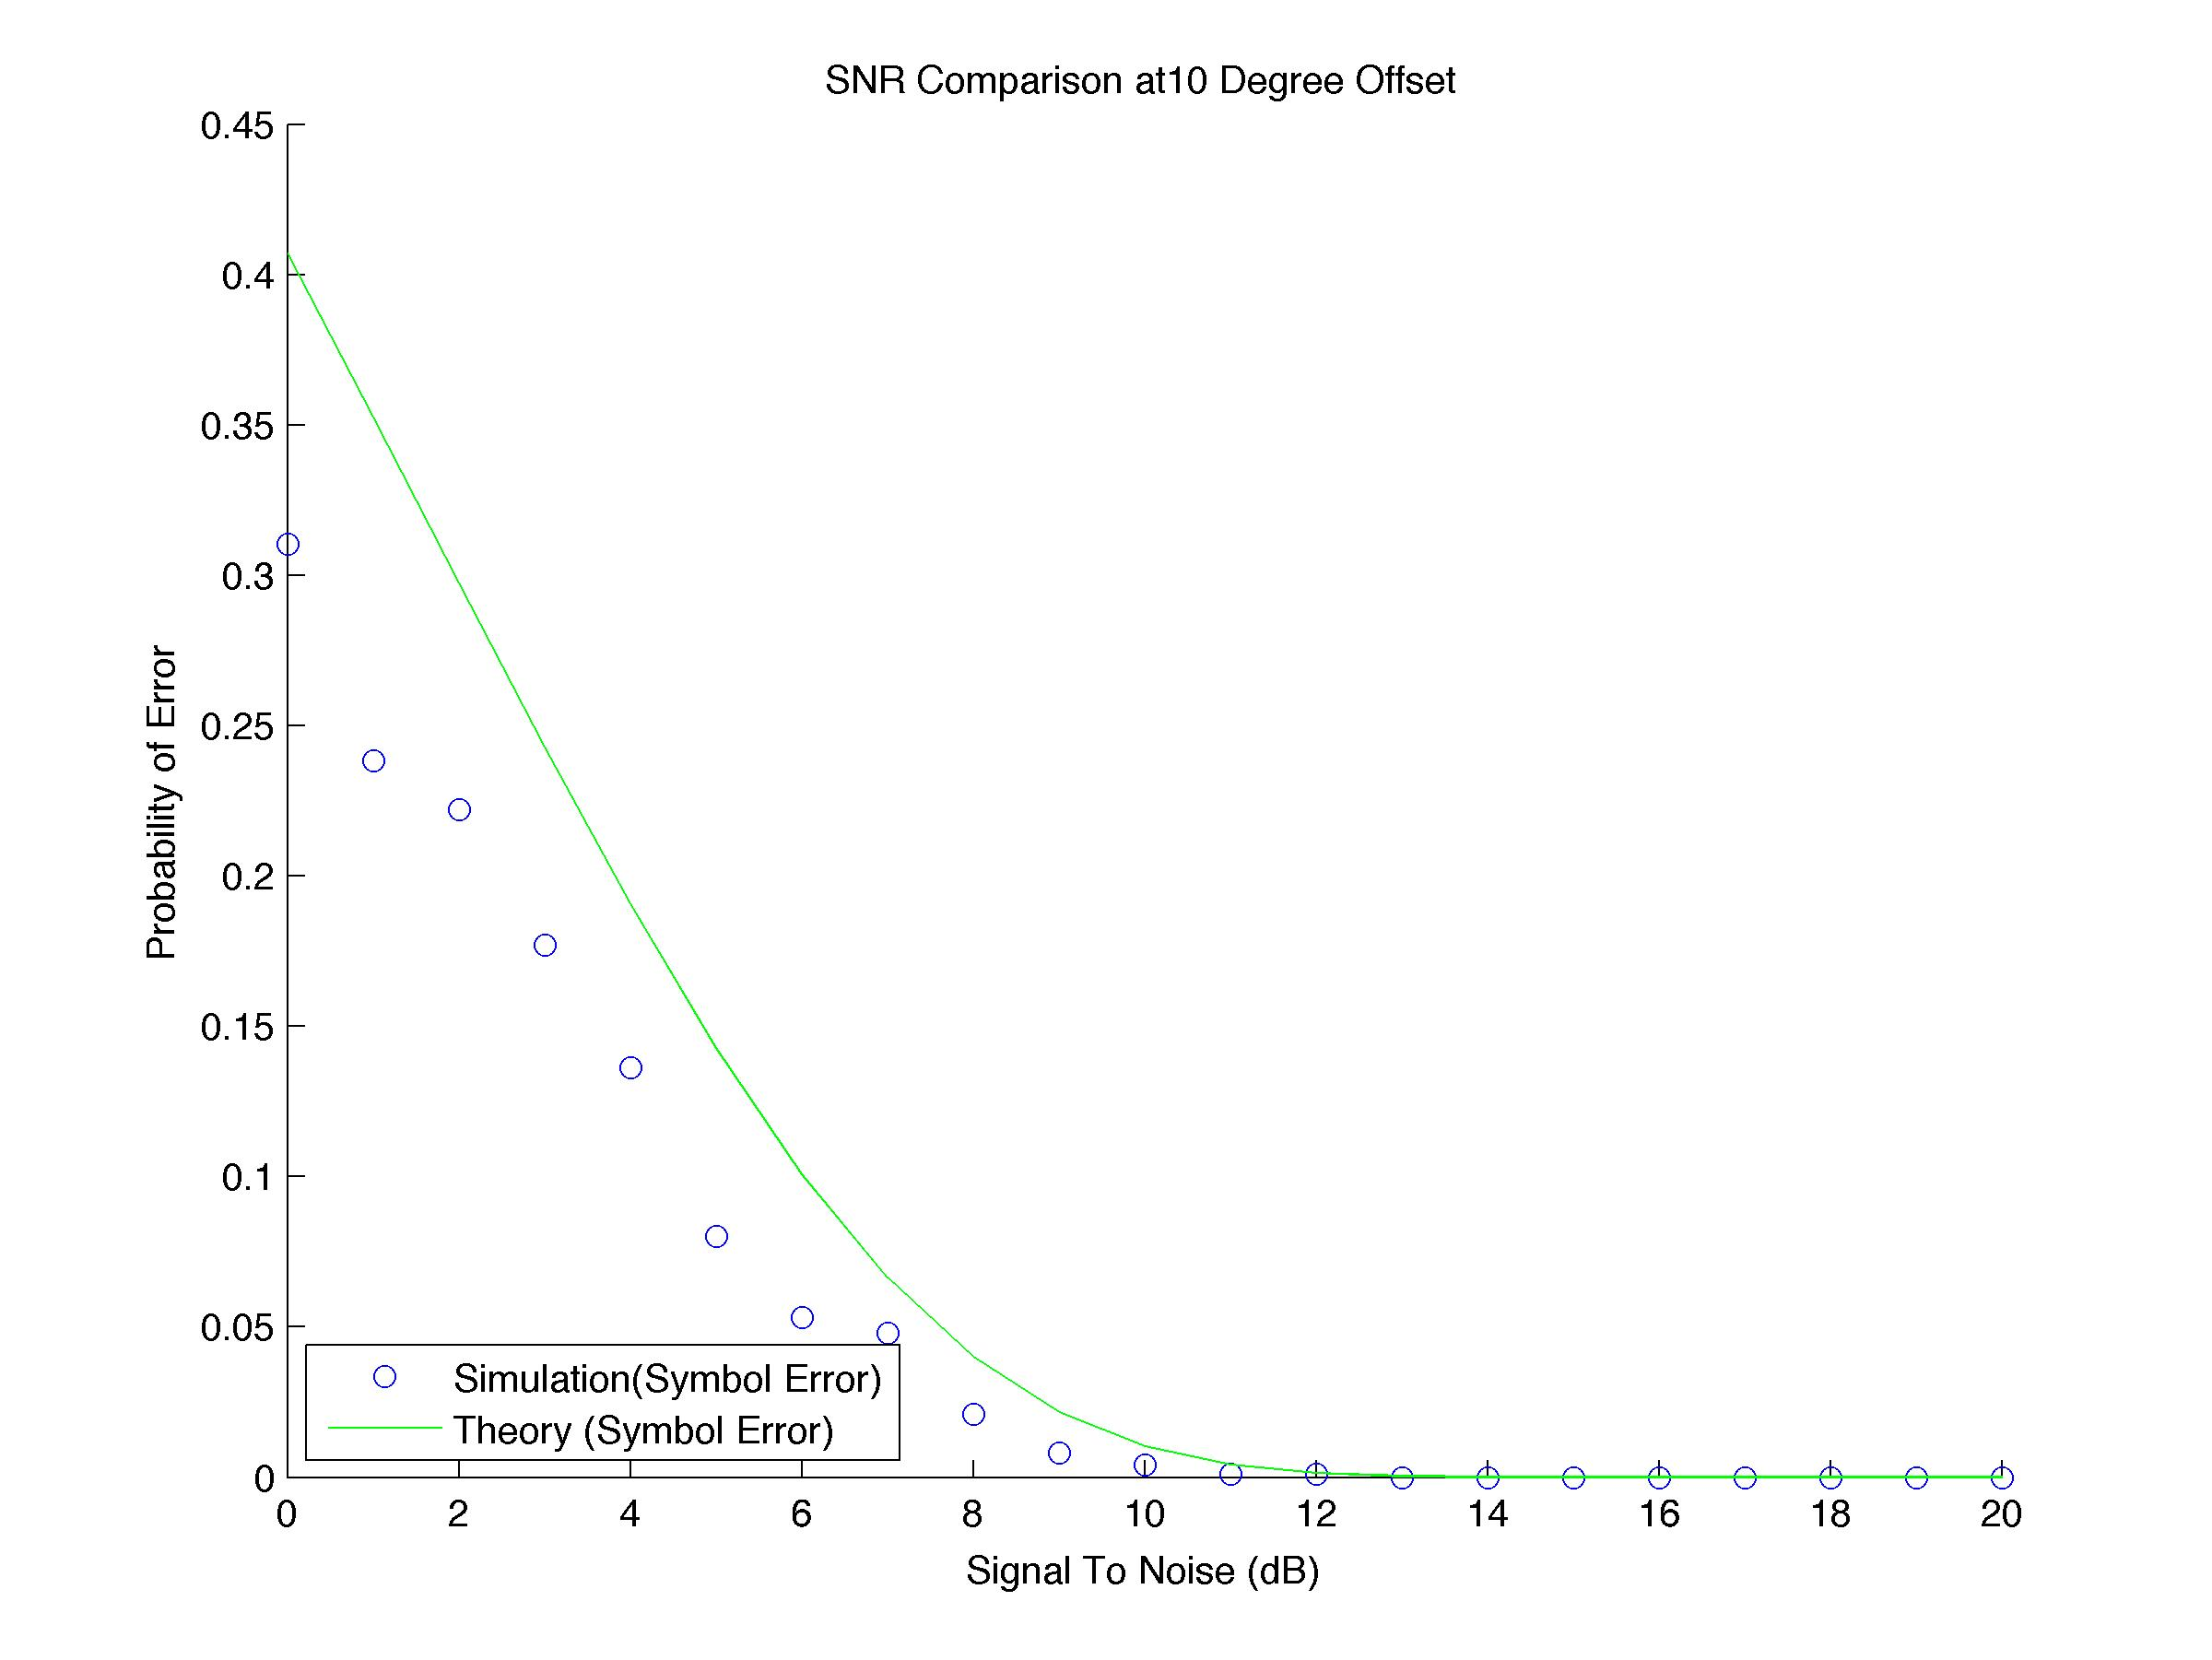
\includegraphics[width=1.3\textwidth]{qpSNRpo2.jpg}
\caption{QPSK Theoretical and Experimental error rates versus different SNR levels at a phase offset of 10 degrees }
\end{figure}

\begin{figure}[H]
\centering
\hspace*{-2cm}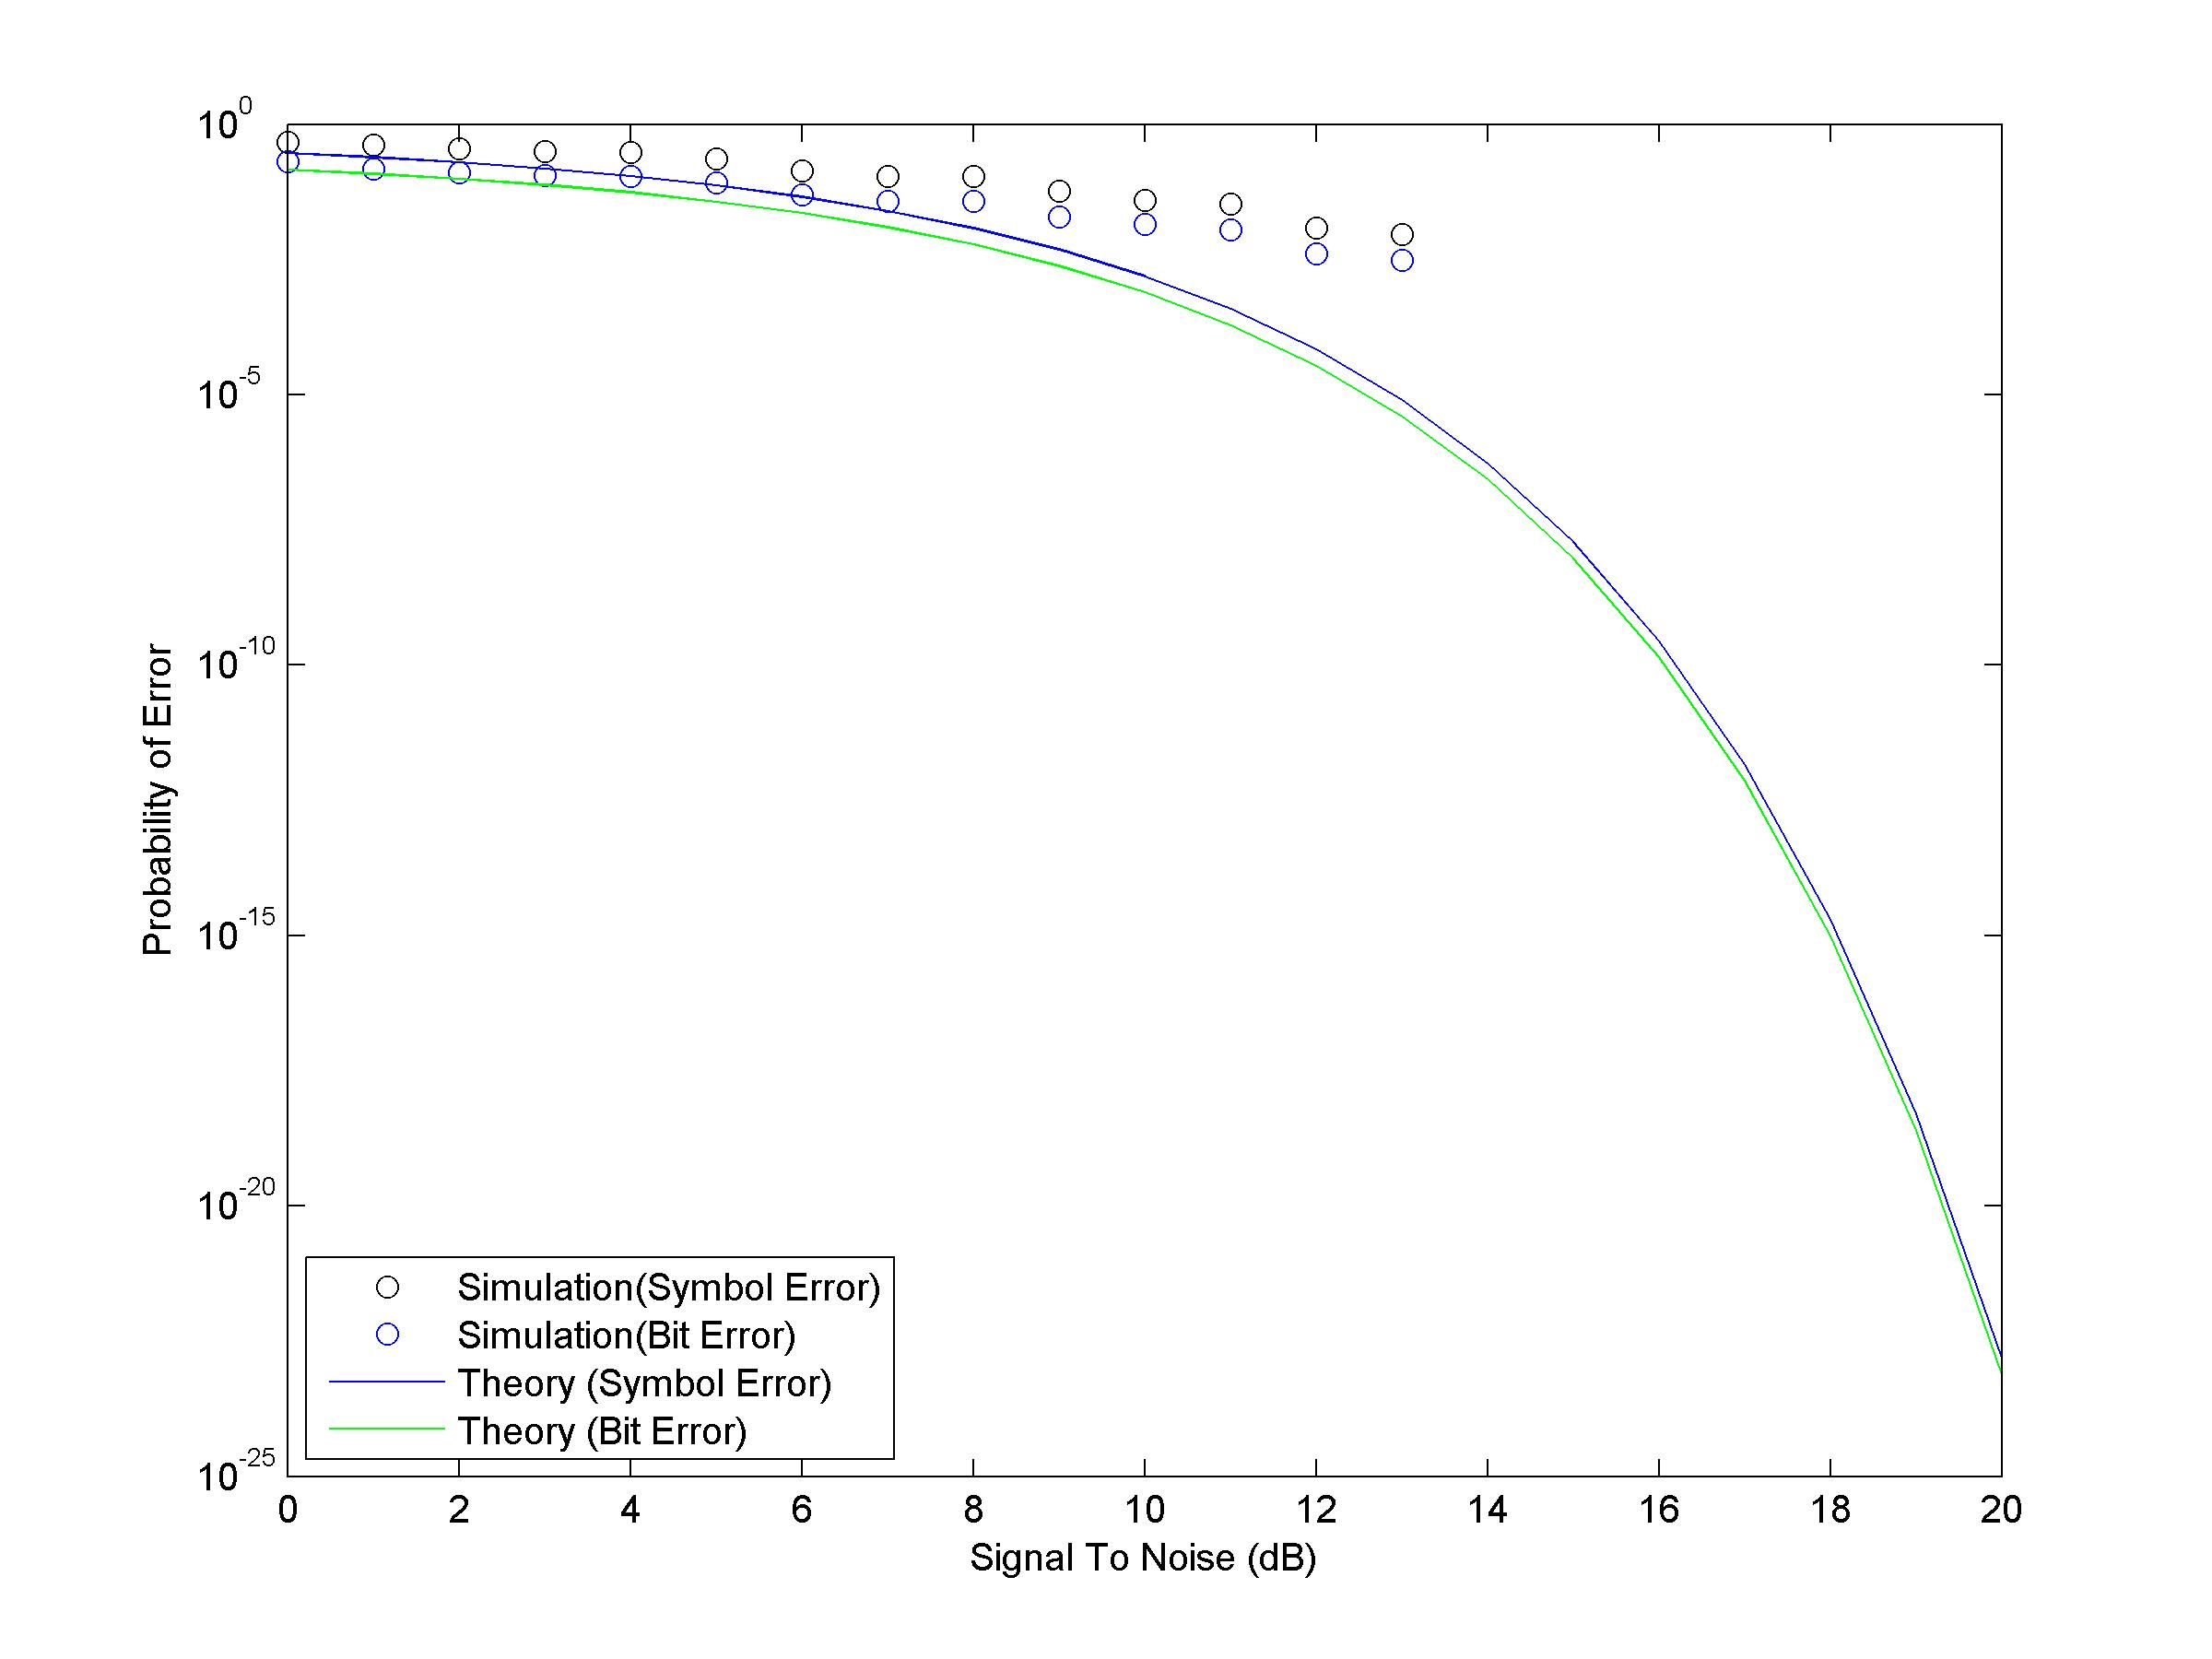
\includegraphics[width=1.3\textwidth]{qpSNRpo3.jpg}
\caption{QPSK Theoretical and Experimental error rates versus different SNR levels at a phase offset of 20 degrees }
\end{figure}

\begin{figure}[H]
\centering
\hspace*{-2cm}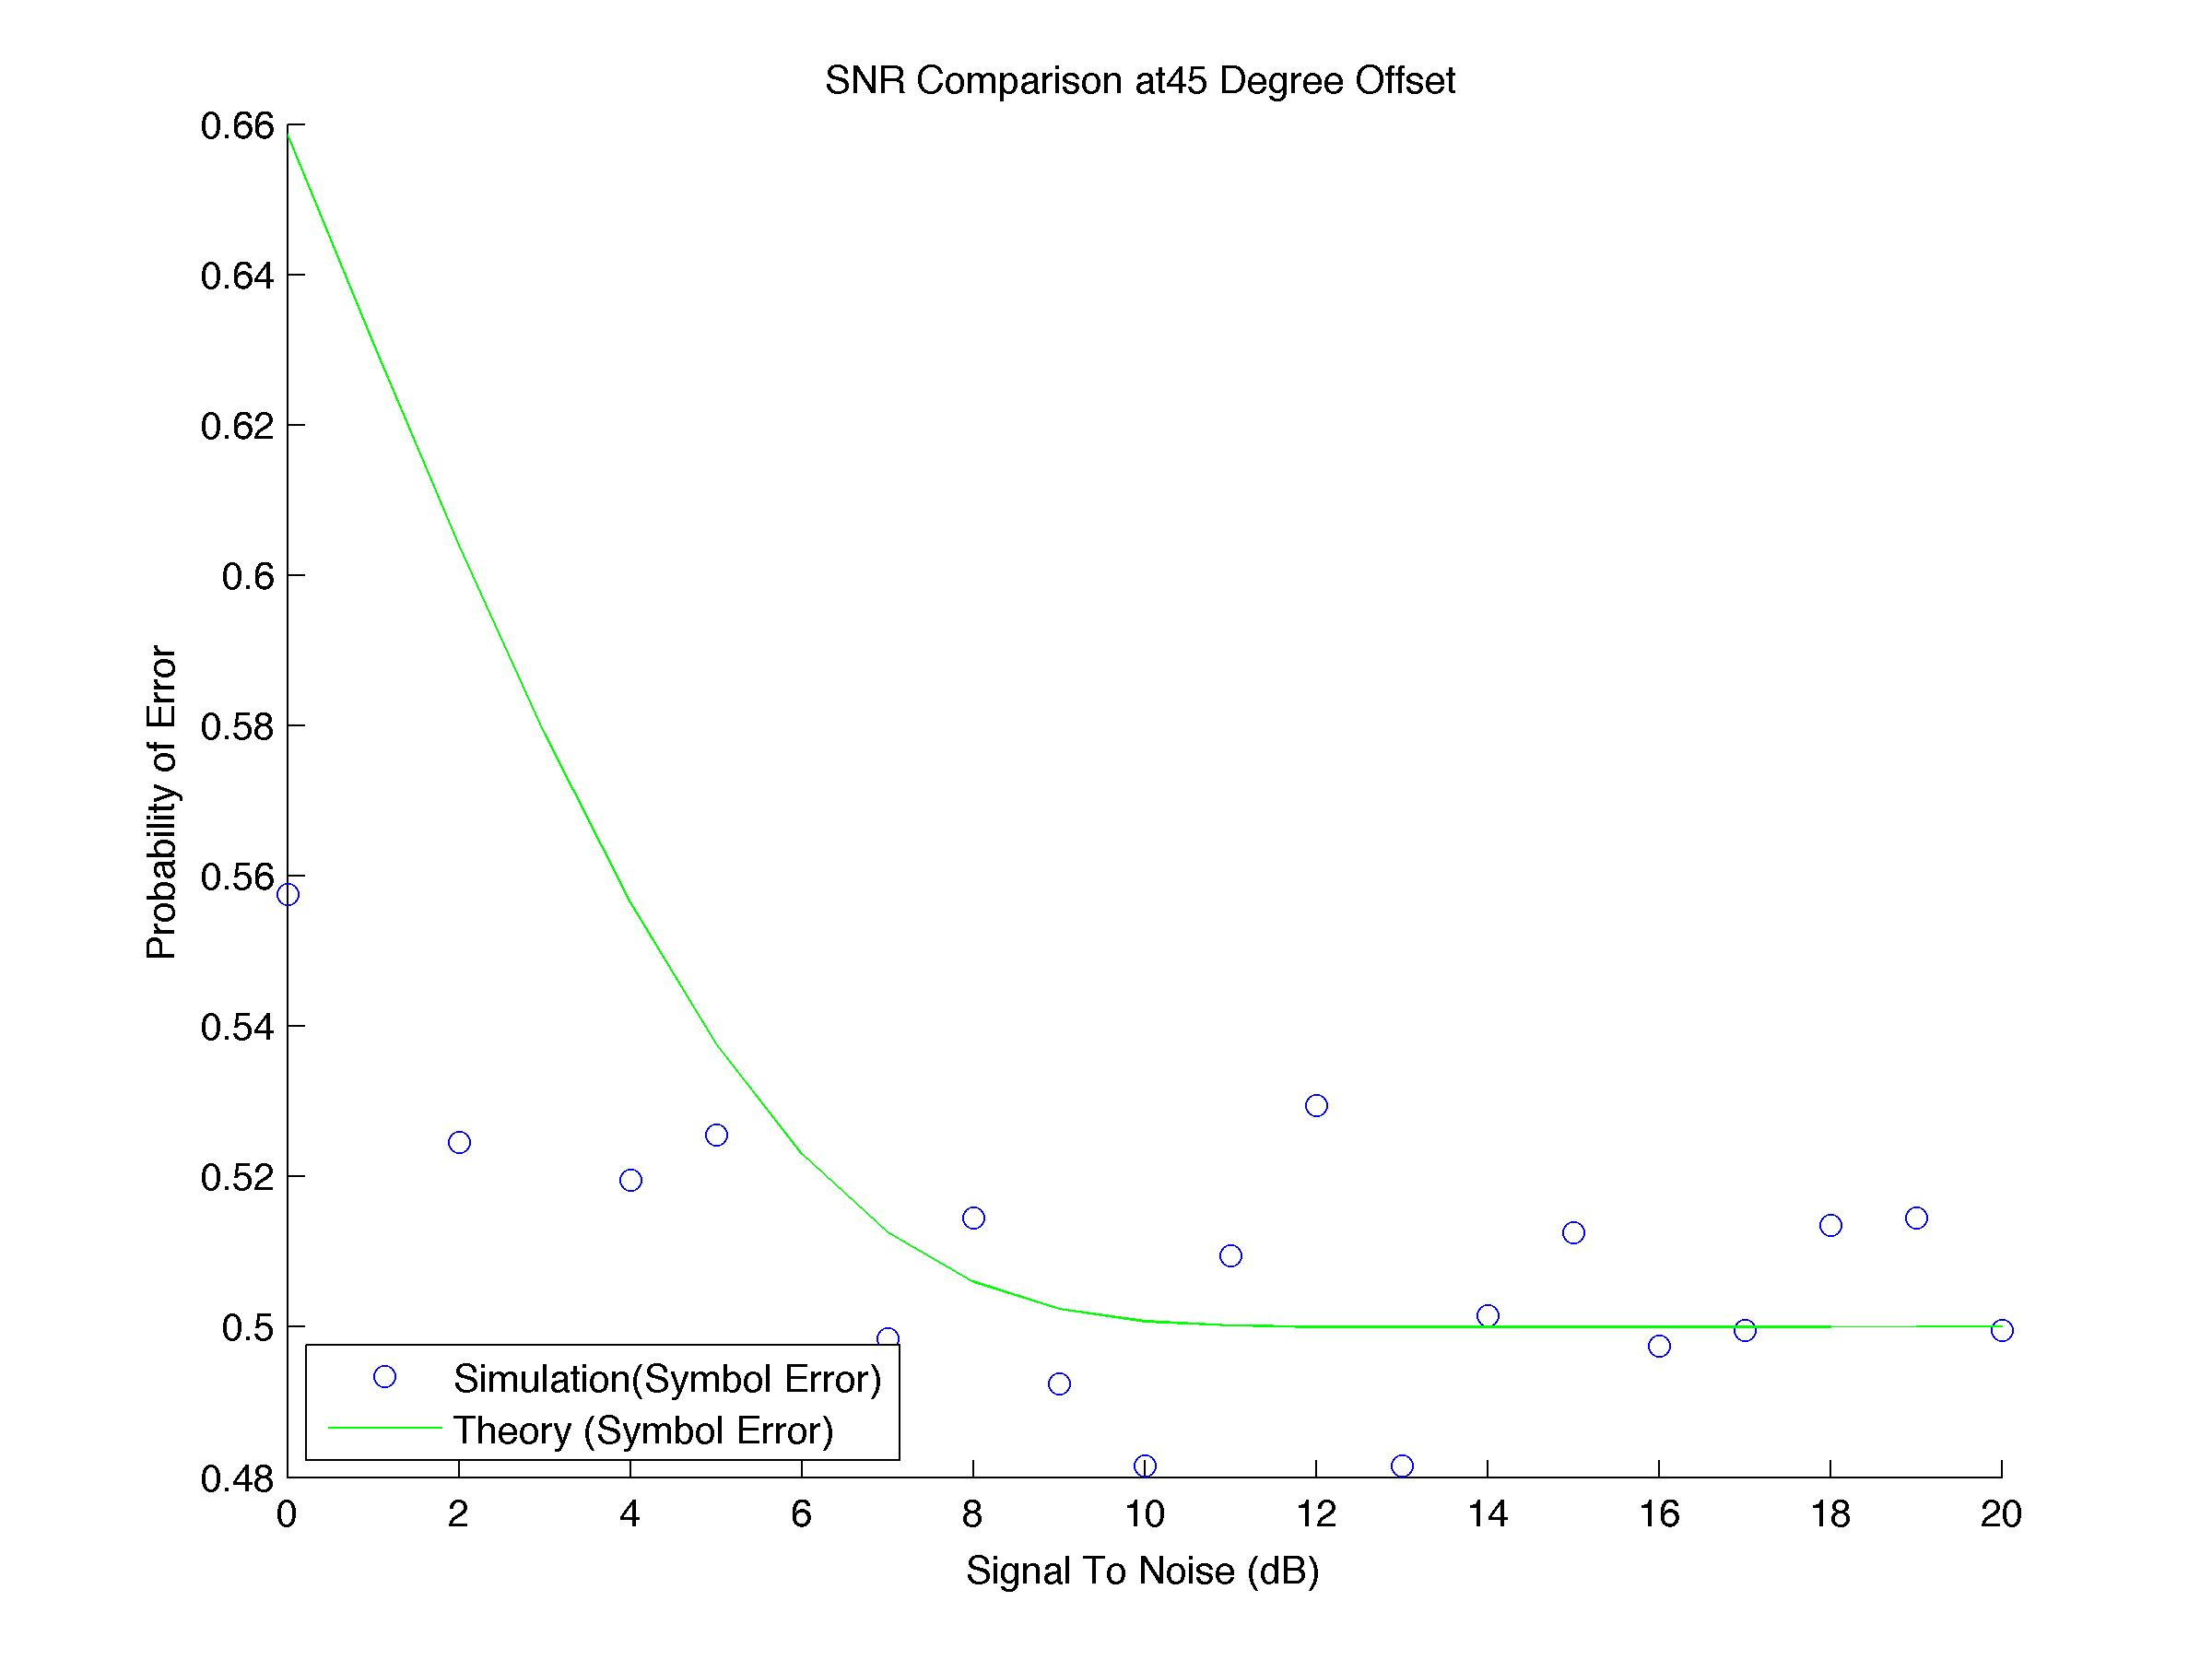
\includegraphics[width=1.3\textwidth]{qpSNRpo4.jpg}
\caption{QPSK Theoretical and Experimental error rates versus different SNR levels at a phase offset of 45 degrees }
\end{figure}


\subsubsection{16-QAM with Phase Offset}
\label{qam16_phase}
\begin{figure}[H]
\centering
\hspace*{-2cm}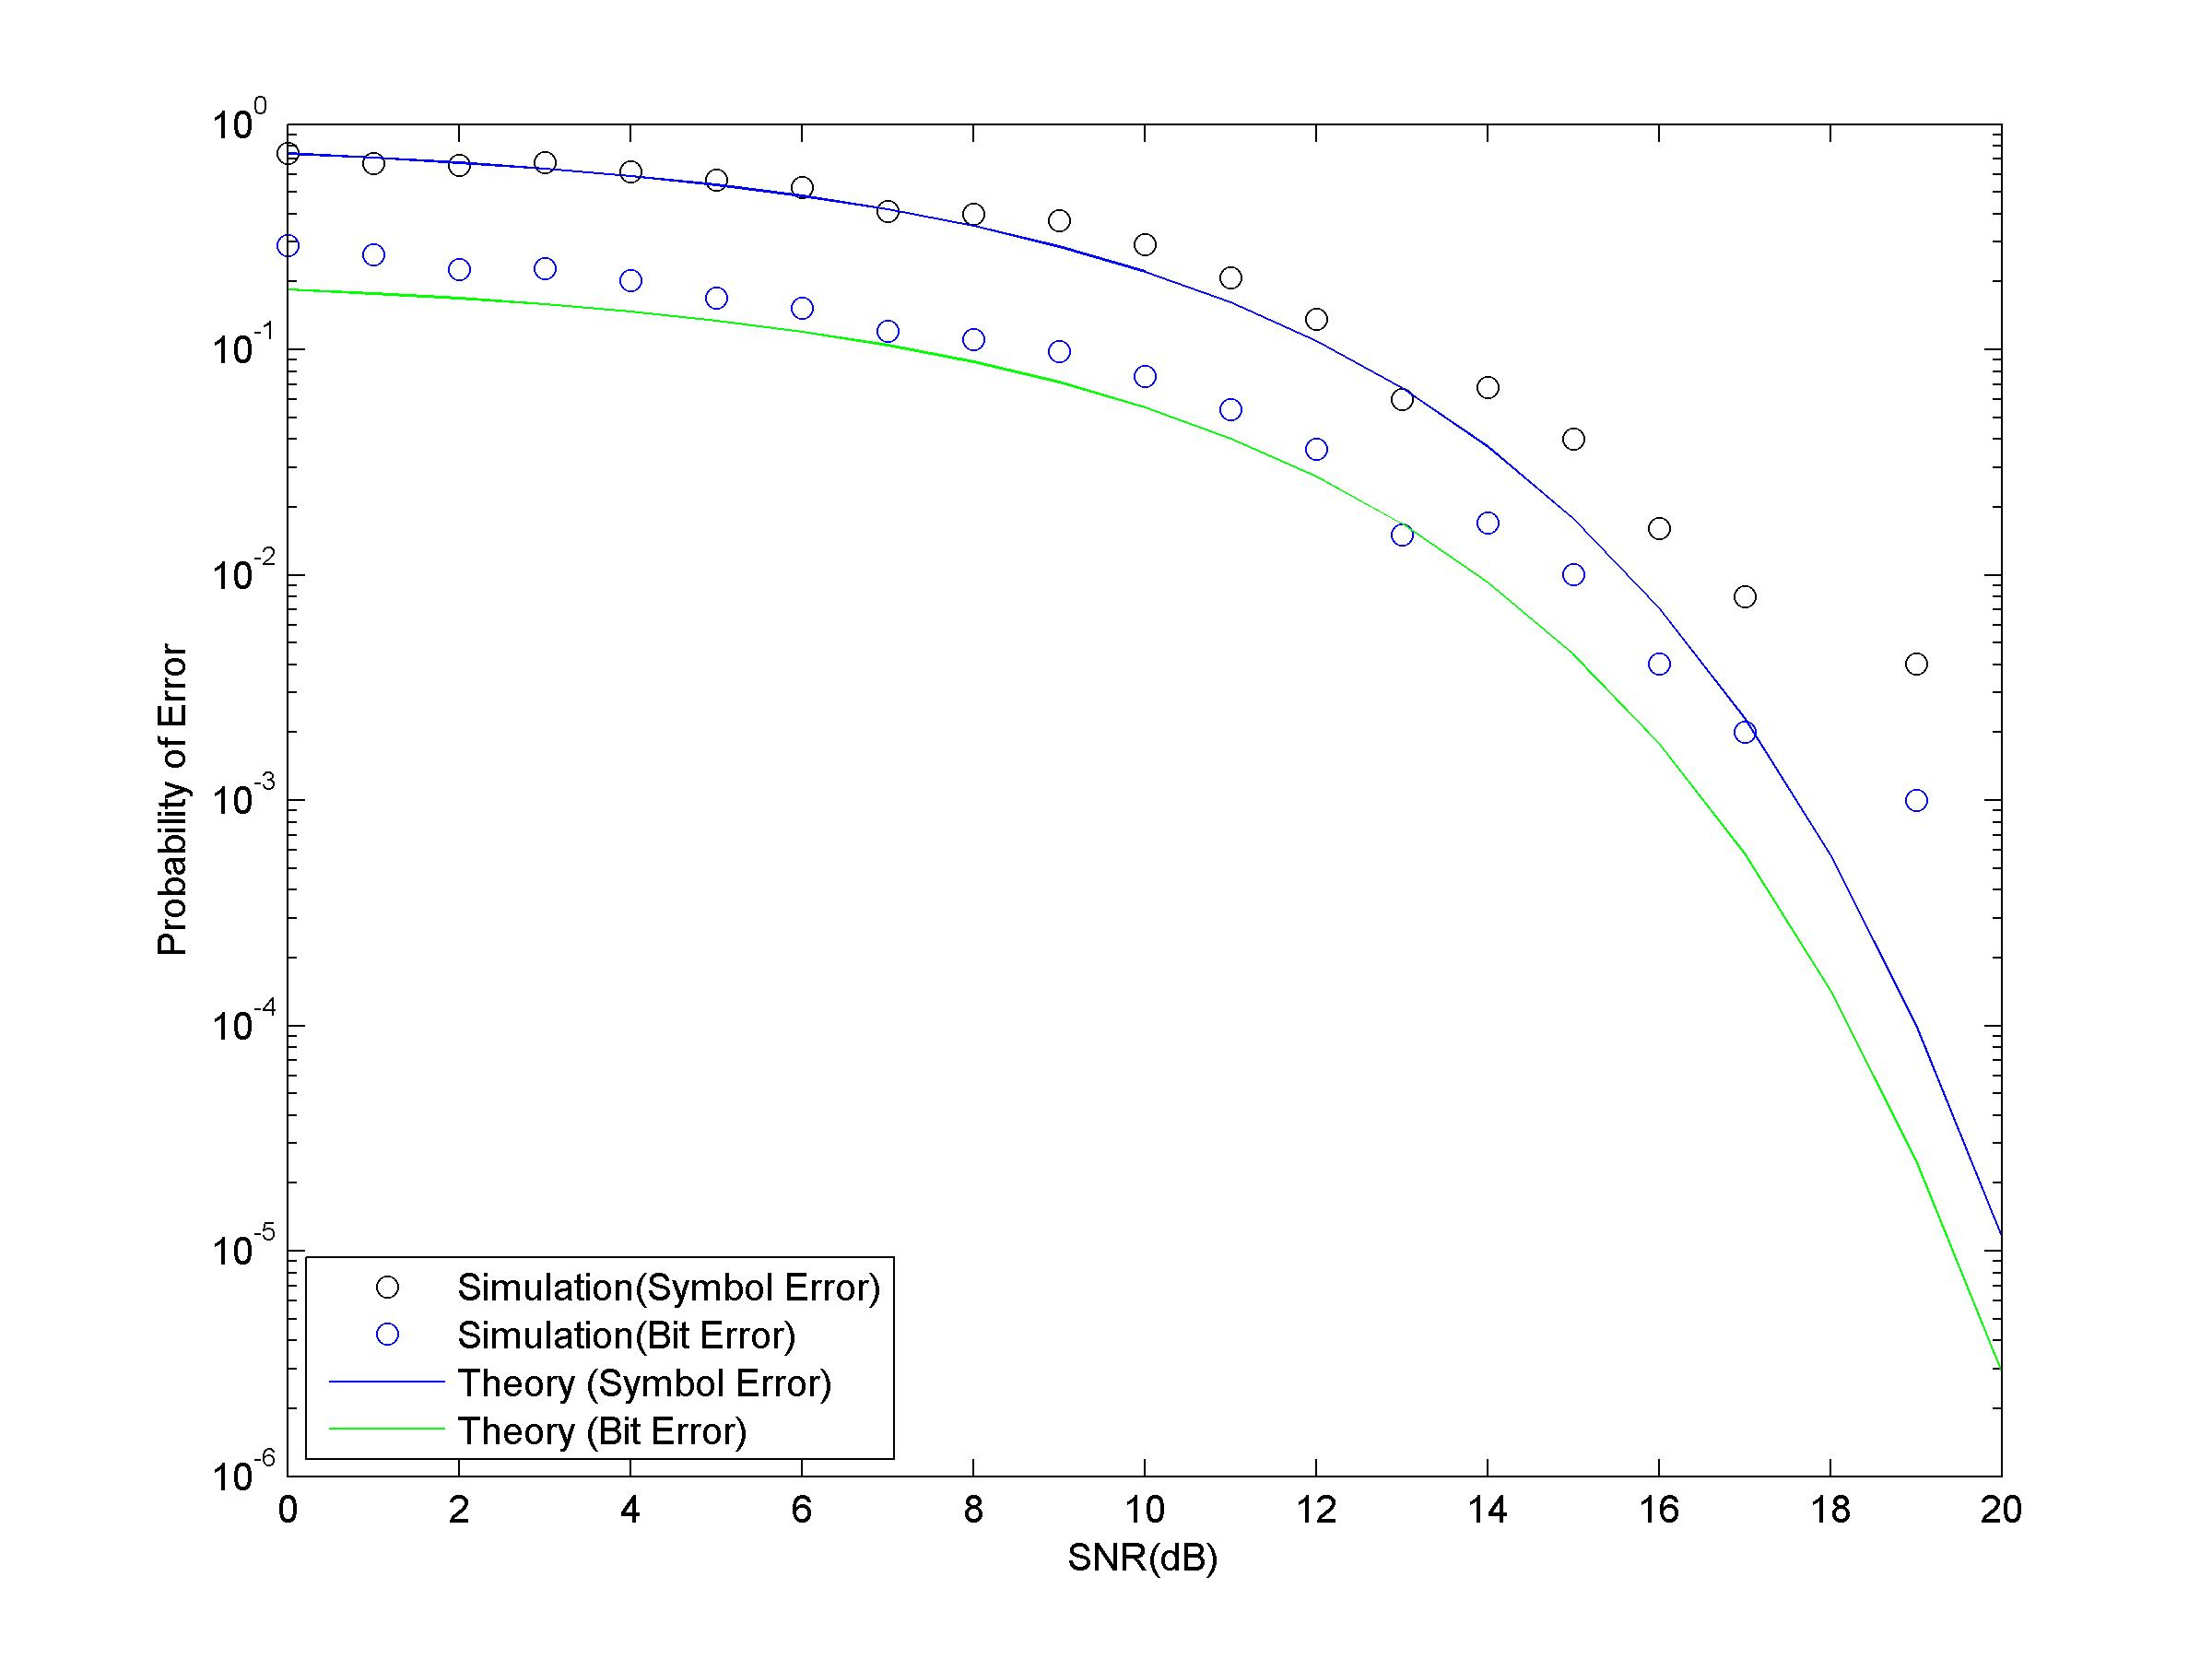
\includegraphics[width=1.3\textwidth]{qam16SNRpo1.jpg}
\caption{16-QAM Theoretical and Experimental error rates versus different SNR levels at a phase offset of 5 degrees }
\end{figure}

\begin{figure}[H]
\centering
\hspace*{-2cm}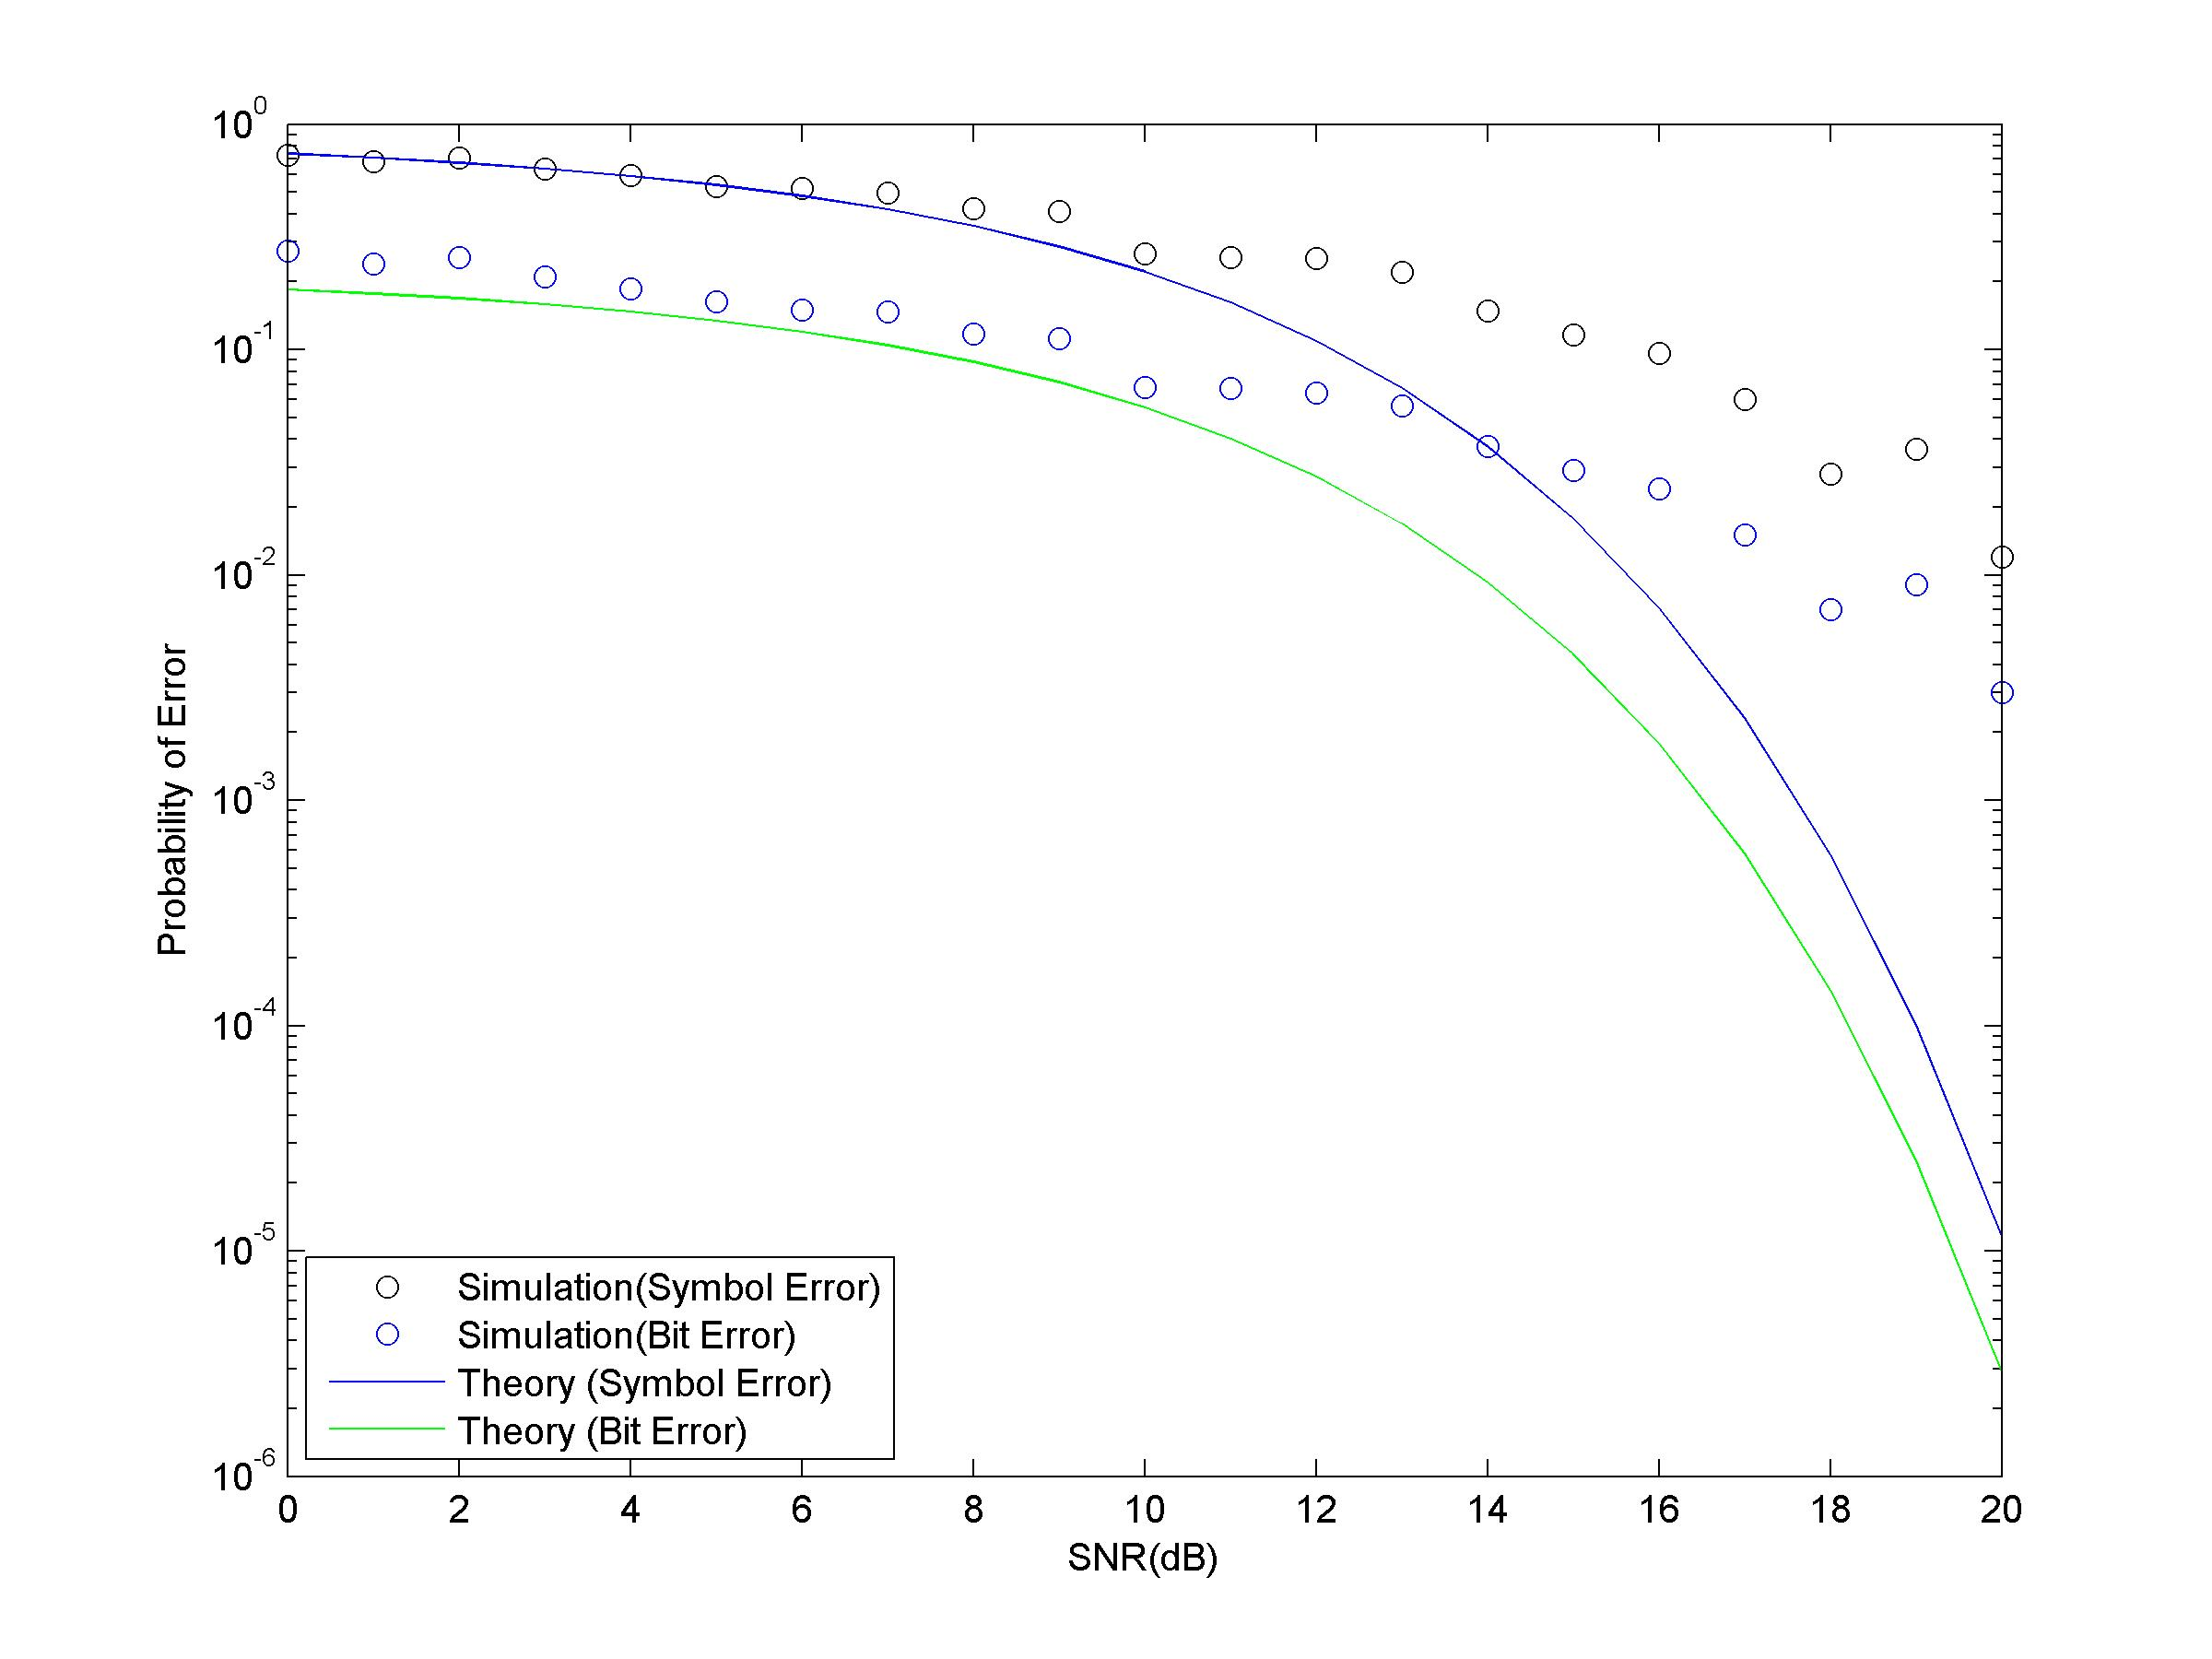
\includegraphics[width=1.3\textwidth]{qam16SNRpo2.jpg}
\caption{16-QAM Theoretical and Experimental error rates versus different SNR levels at a phase offset of 10 degrees }
\end{figure}

\begin{figure}[H]
\centering
\hspace*{-2cm}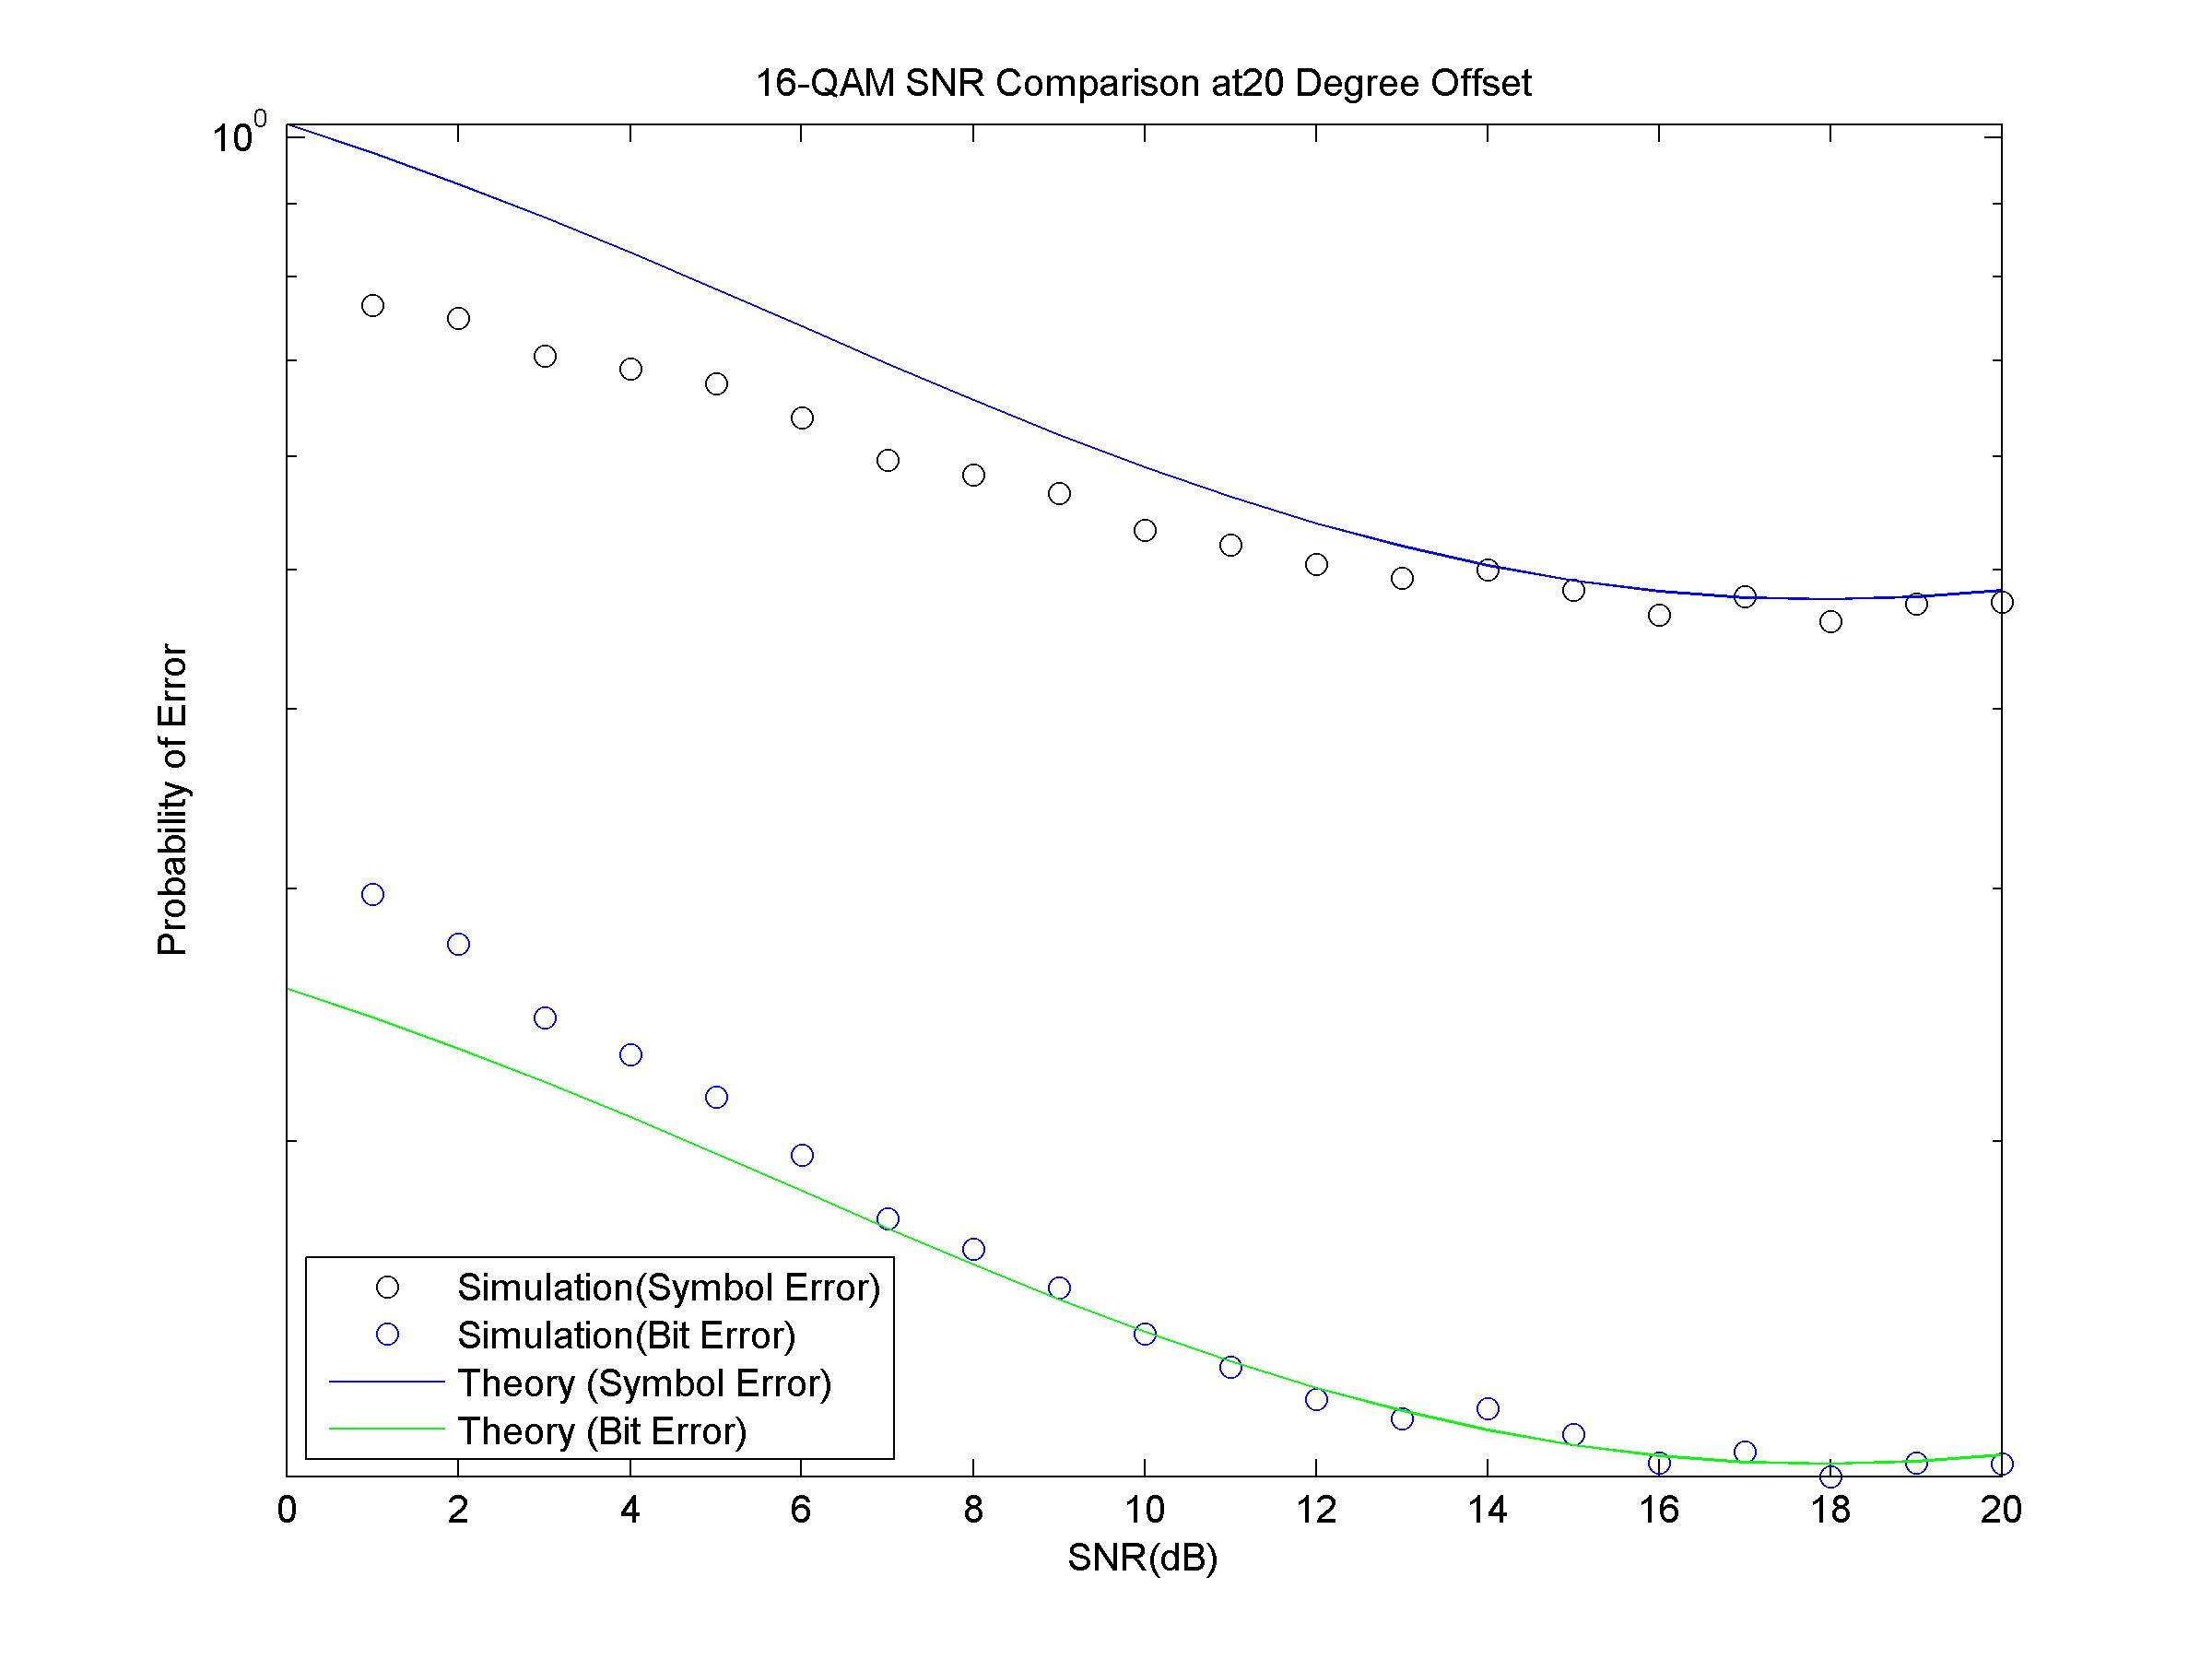
\includegraphics[width=1.3\textwidth]{qam16SNRpo3.jpg}
\caption{16-QAM Theoretical and Experimental error rates versus different SNR levels at a phase offset of 20 degrees }
\end{figure}

\begin{figure}[H]
\centering
\hspace*{-2cm}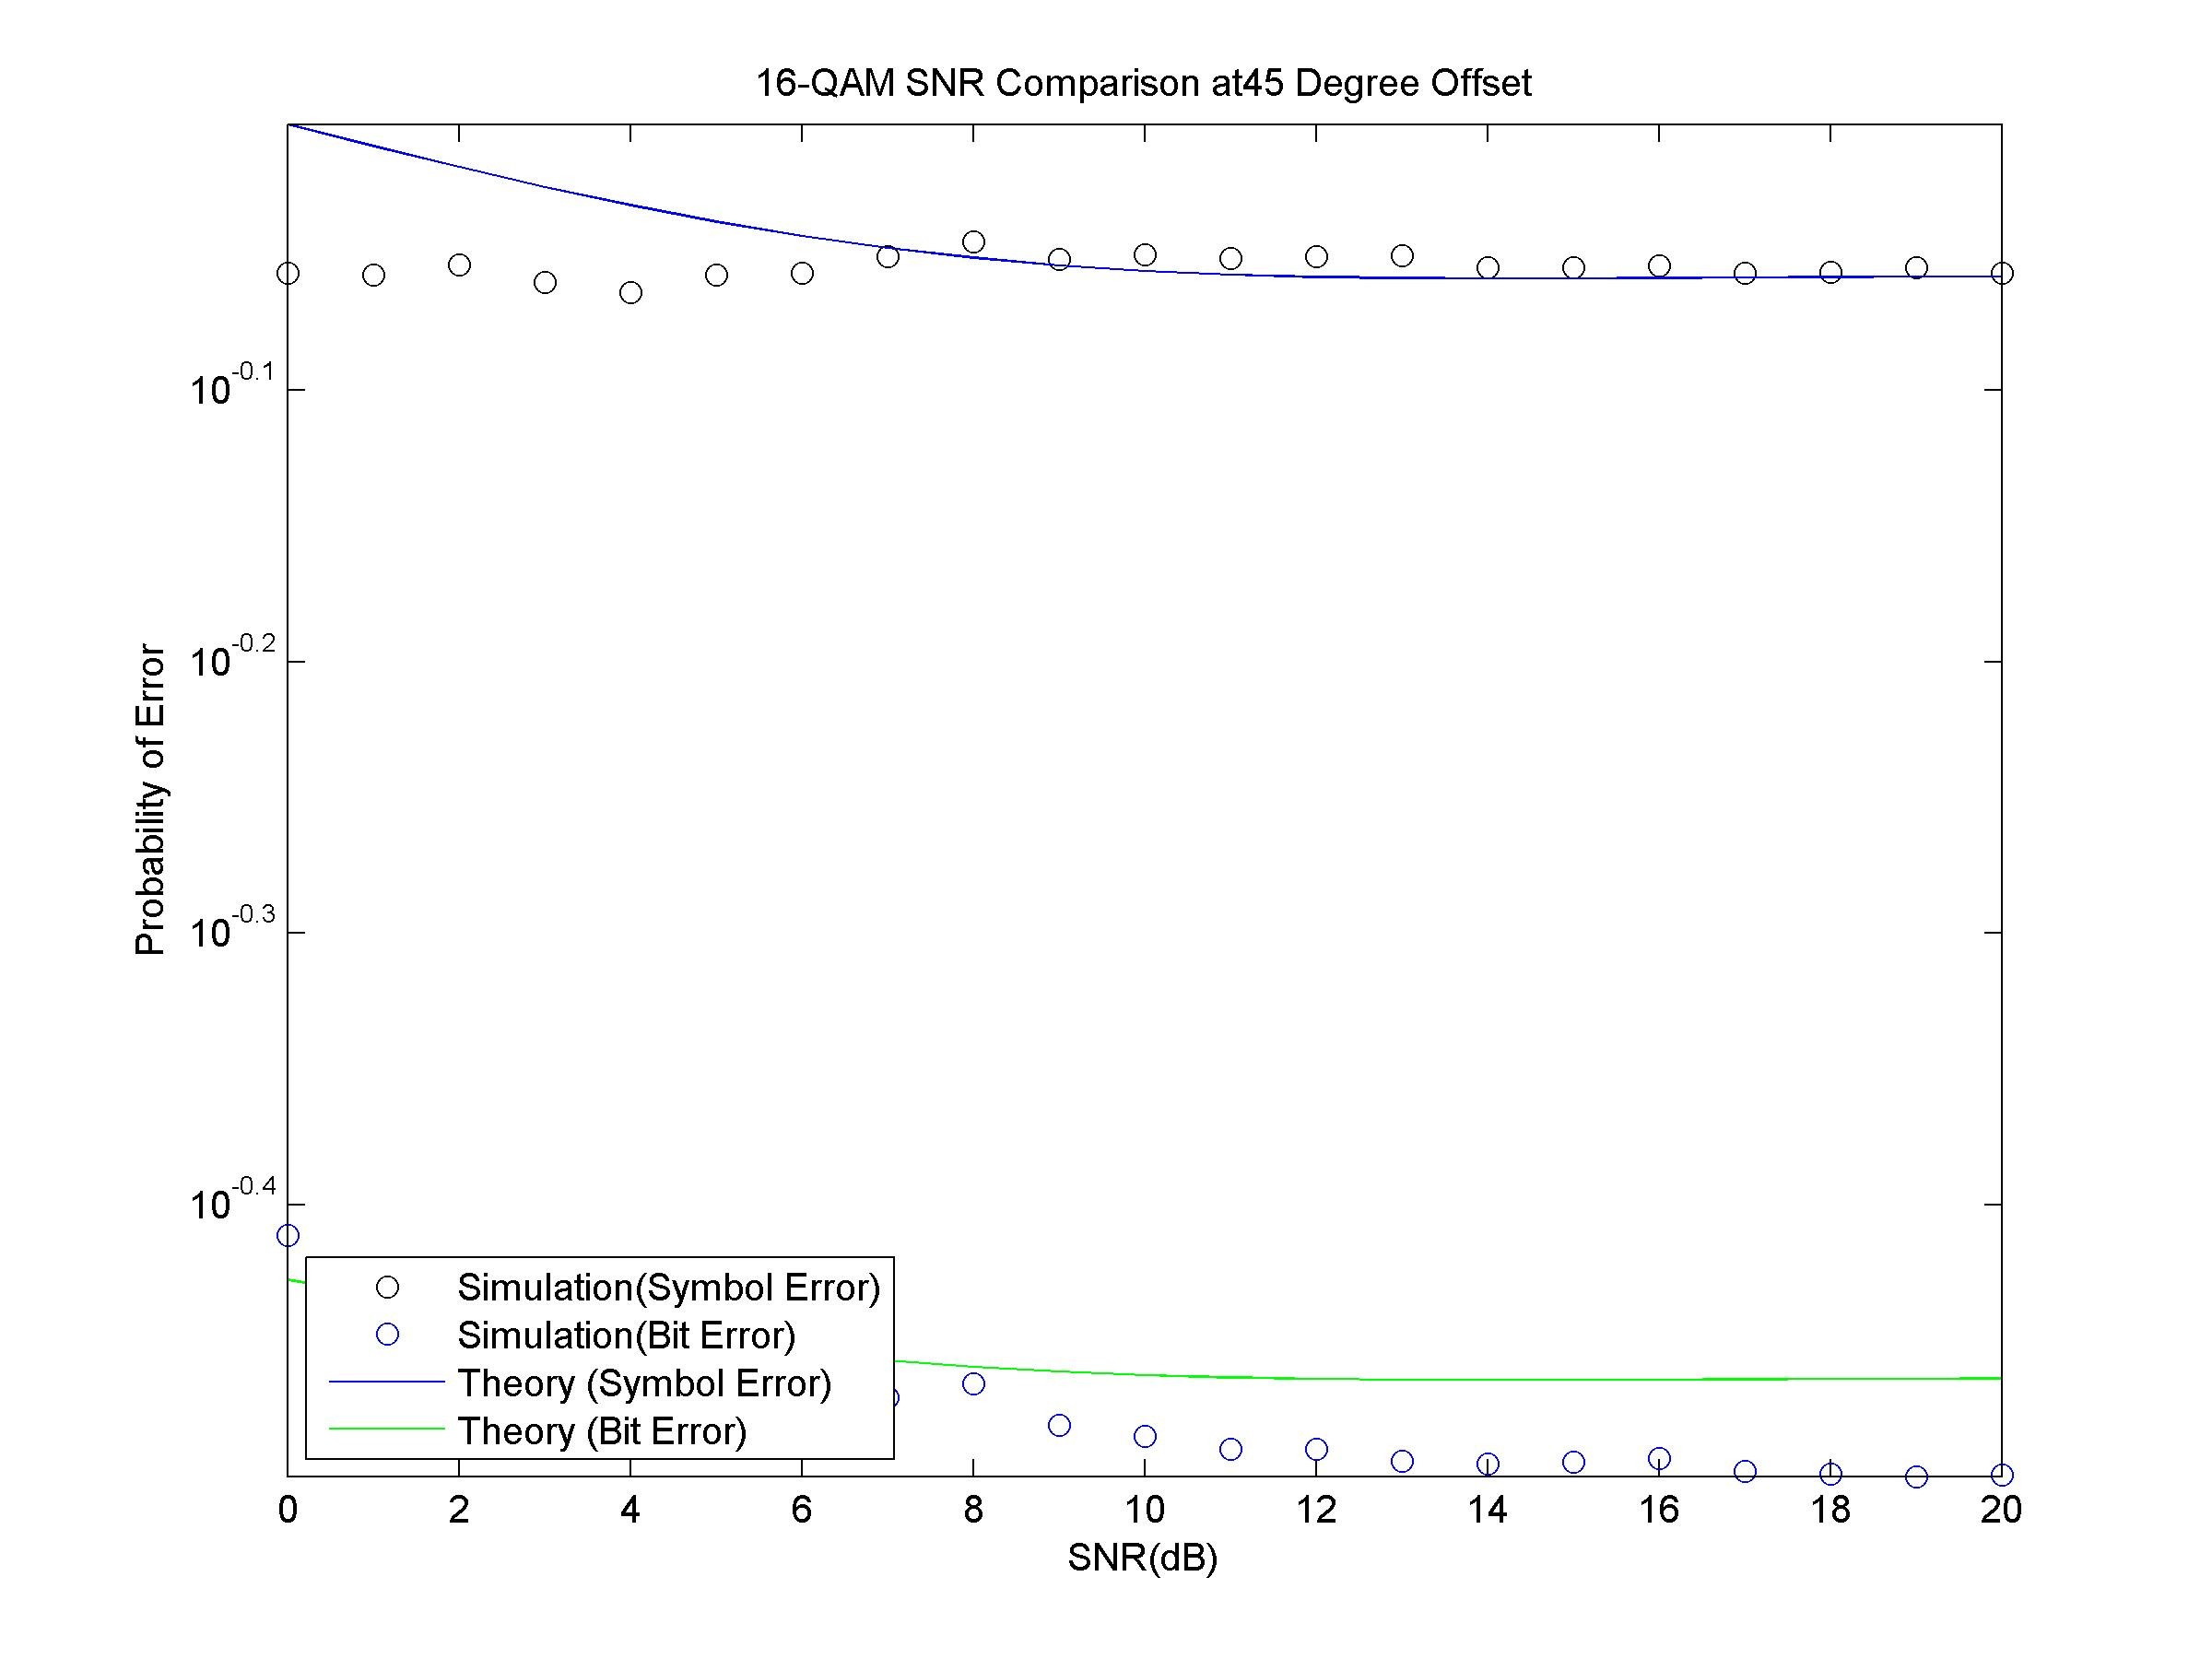
\includegraphics[width=1.3\textwidth]{qam16SNRpo4.jpg}
\caption{16-QAM Theoretical and Experimental error rates versus different SNR levels at a phase offset of 45 degrees }
\end{figure}

\subsubsection{64-QAM with Phase Offset}
\label{qam64_phase}
\begin{figure}[H]
\centering
\hspace*{-2cm}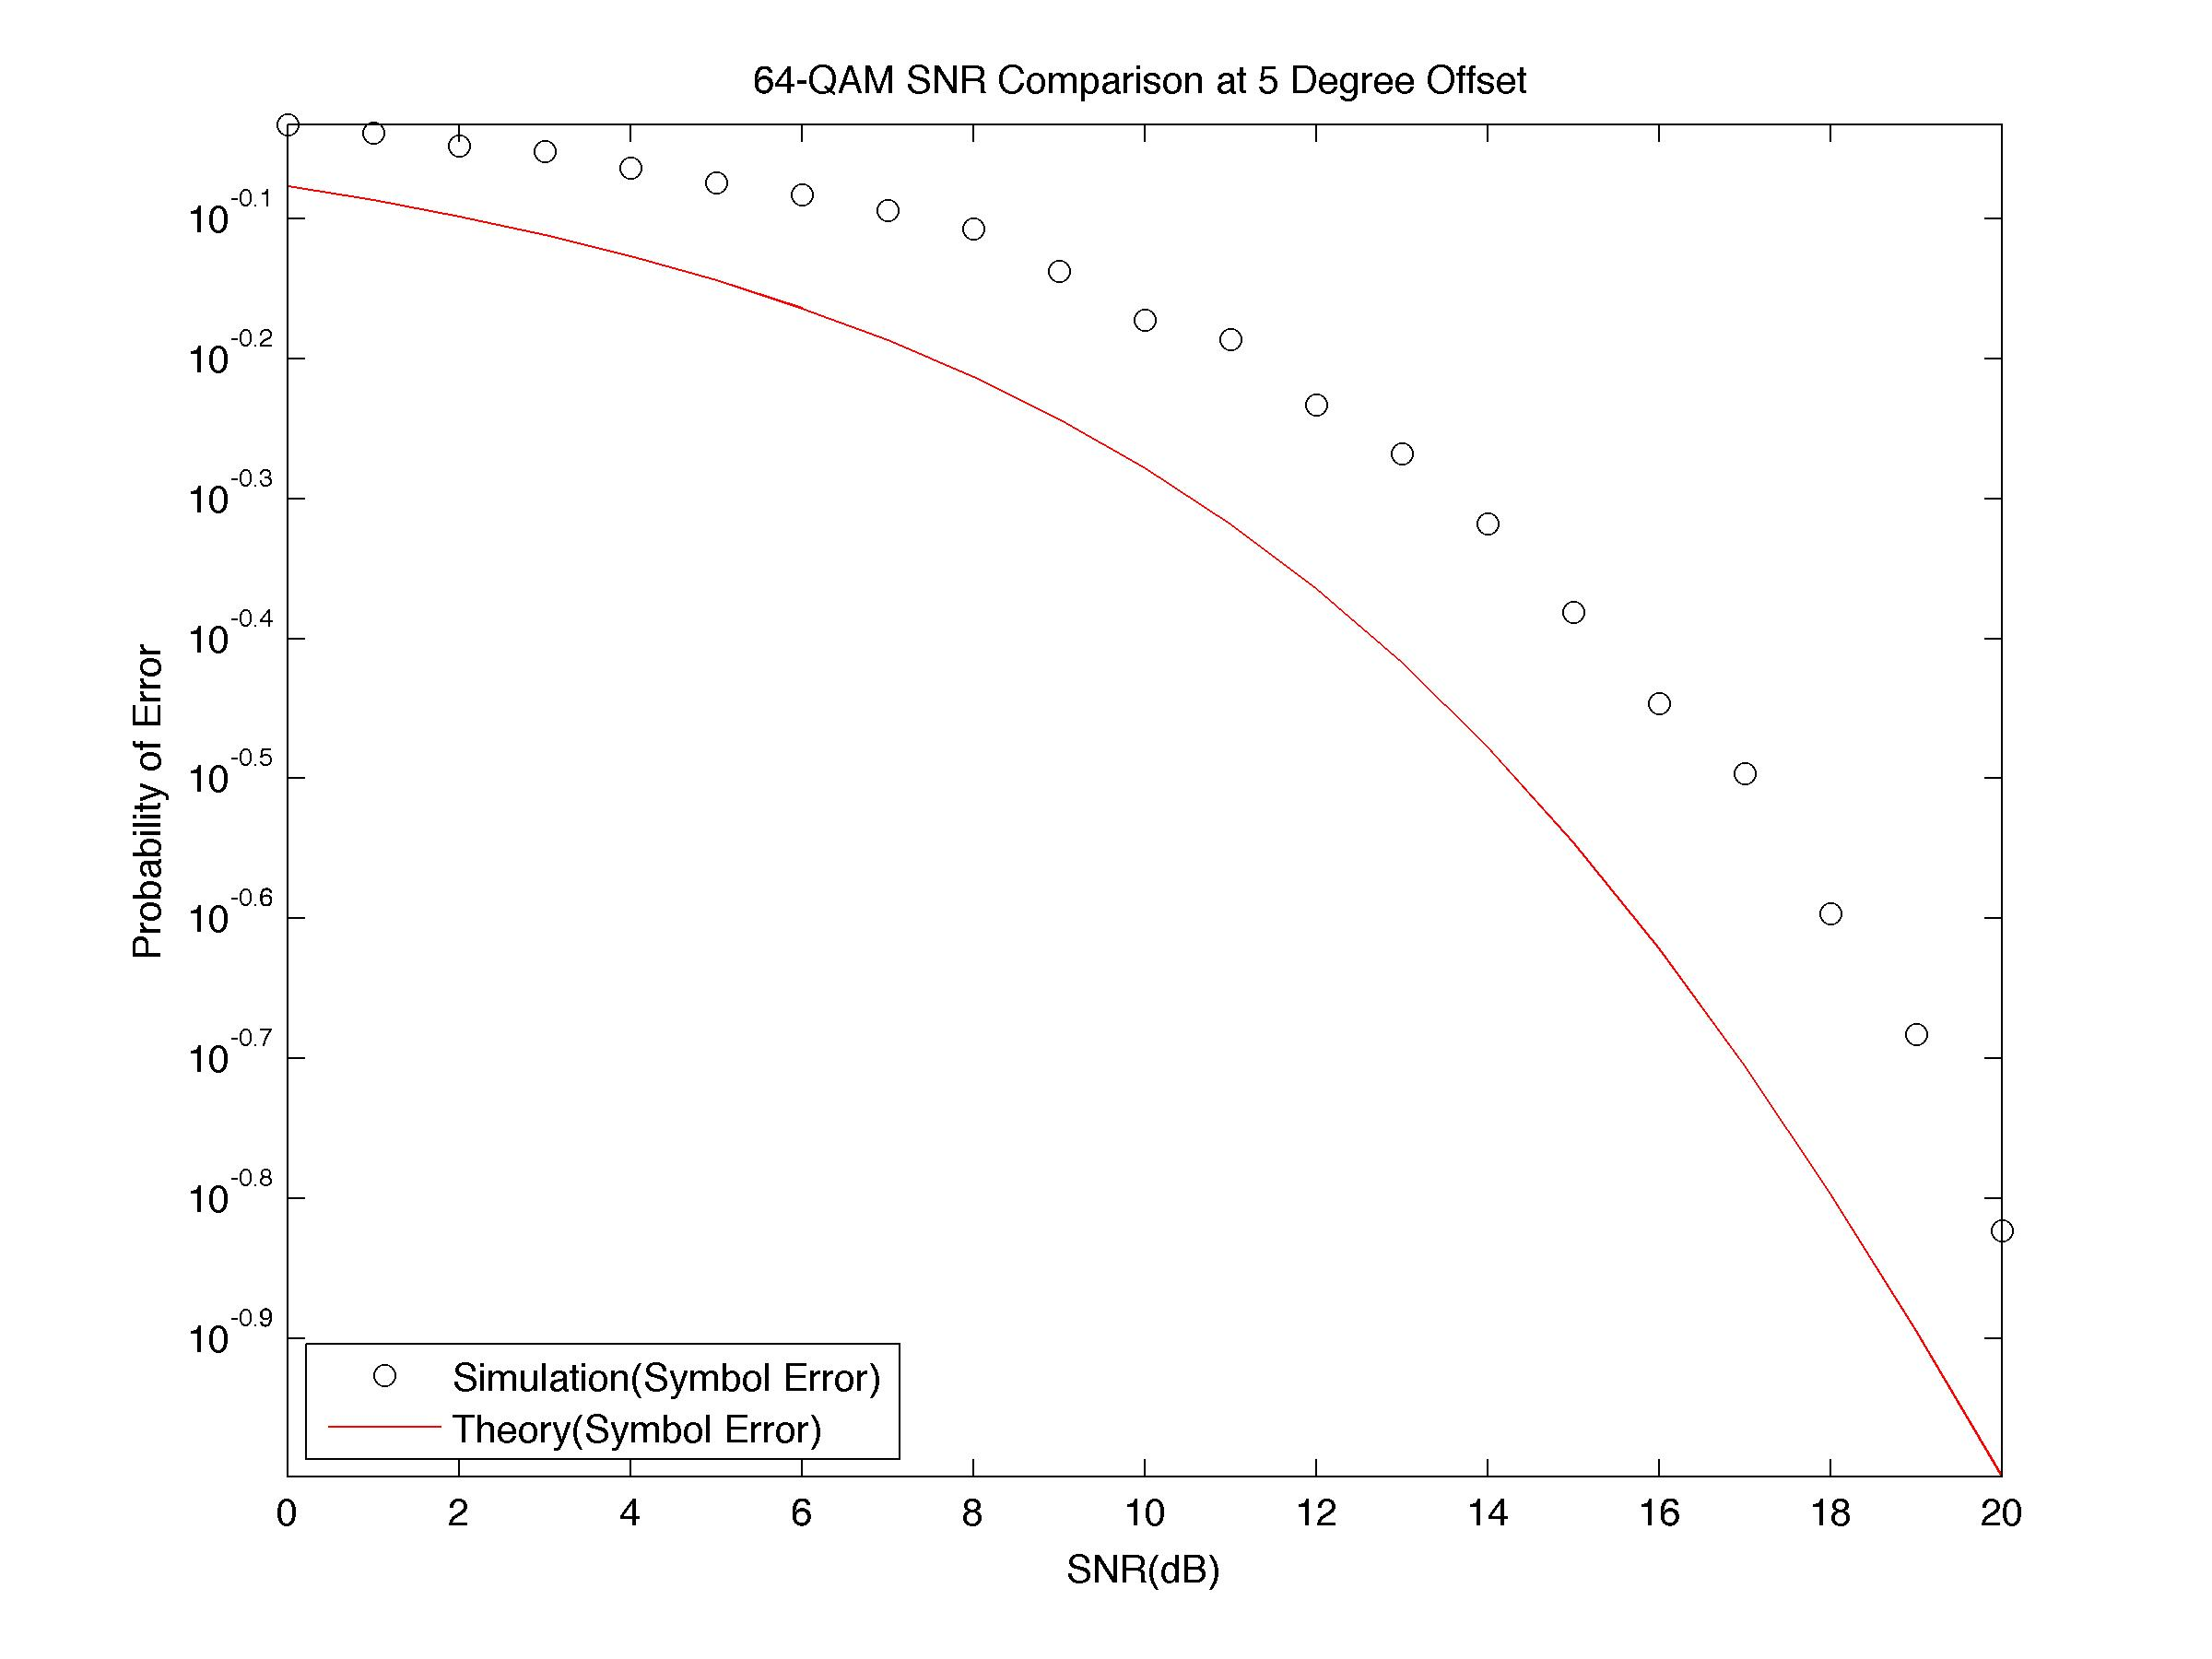
\includegraphics[width=1.3\textwidth]{qam64SNRpo1.jpg}
\caption{64-QAM Theoretical and Experimental error rates versus different SNR levels at a phase offset of 5 degrees }
\end{figure}

\begin{figure}[H]
\centering
\hspace*{-2cm}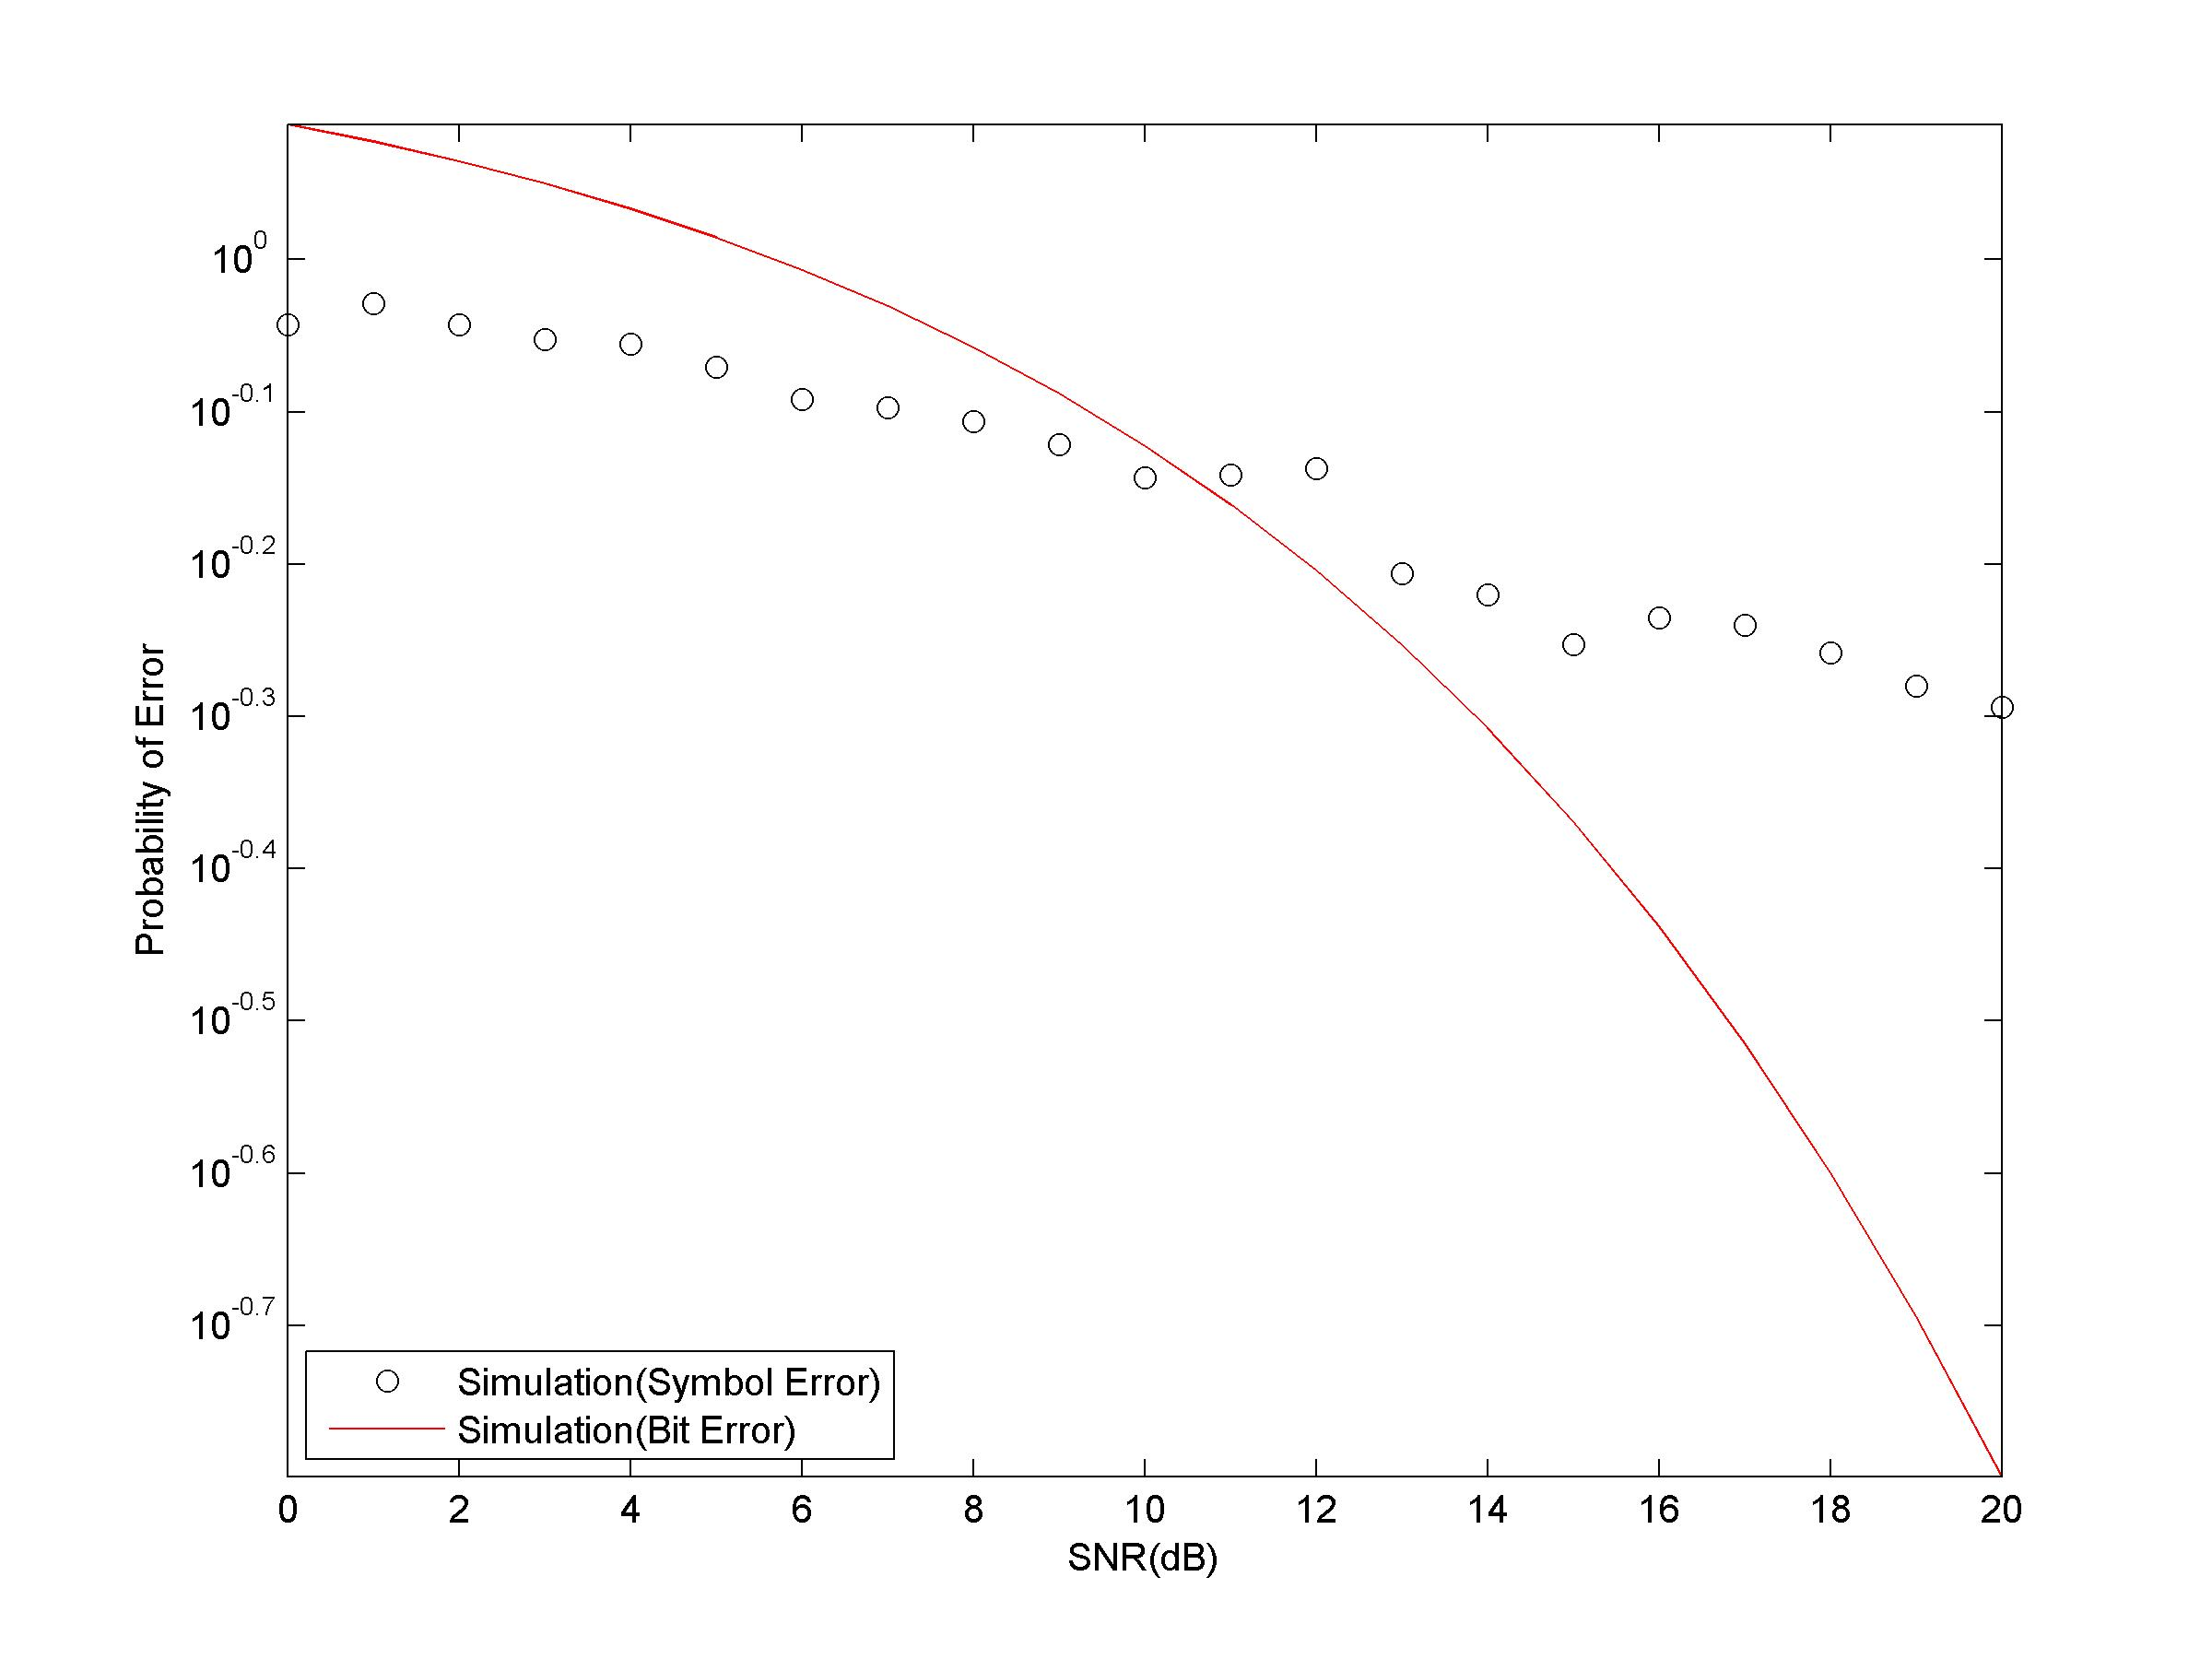
\includegraphics[width=1.3\textwidth]{qam64SNRpo2.jpg}
\caption{64-QAM Theoretical and Experimental error rates versus different SNR levels at a phase offset of 10 degrees }
\end{figure}

\begin{figure}[H]
\centering
\hspace*{-2cm}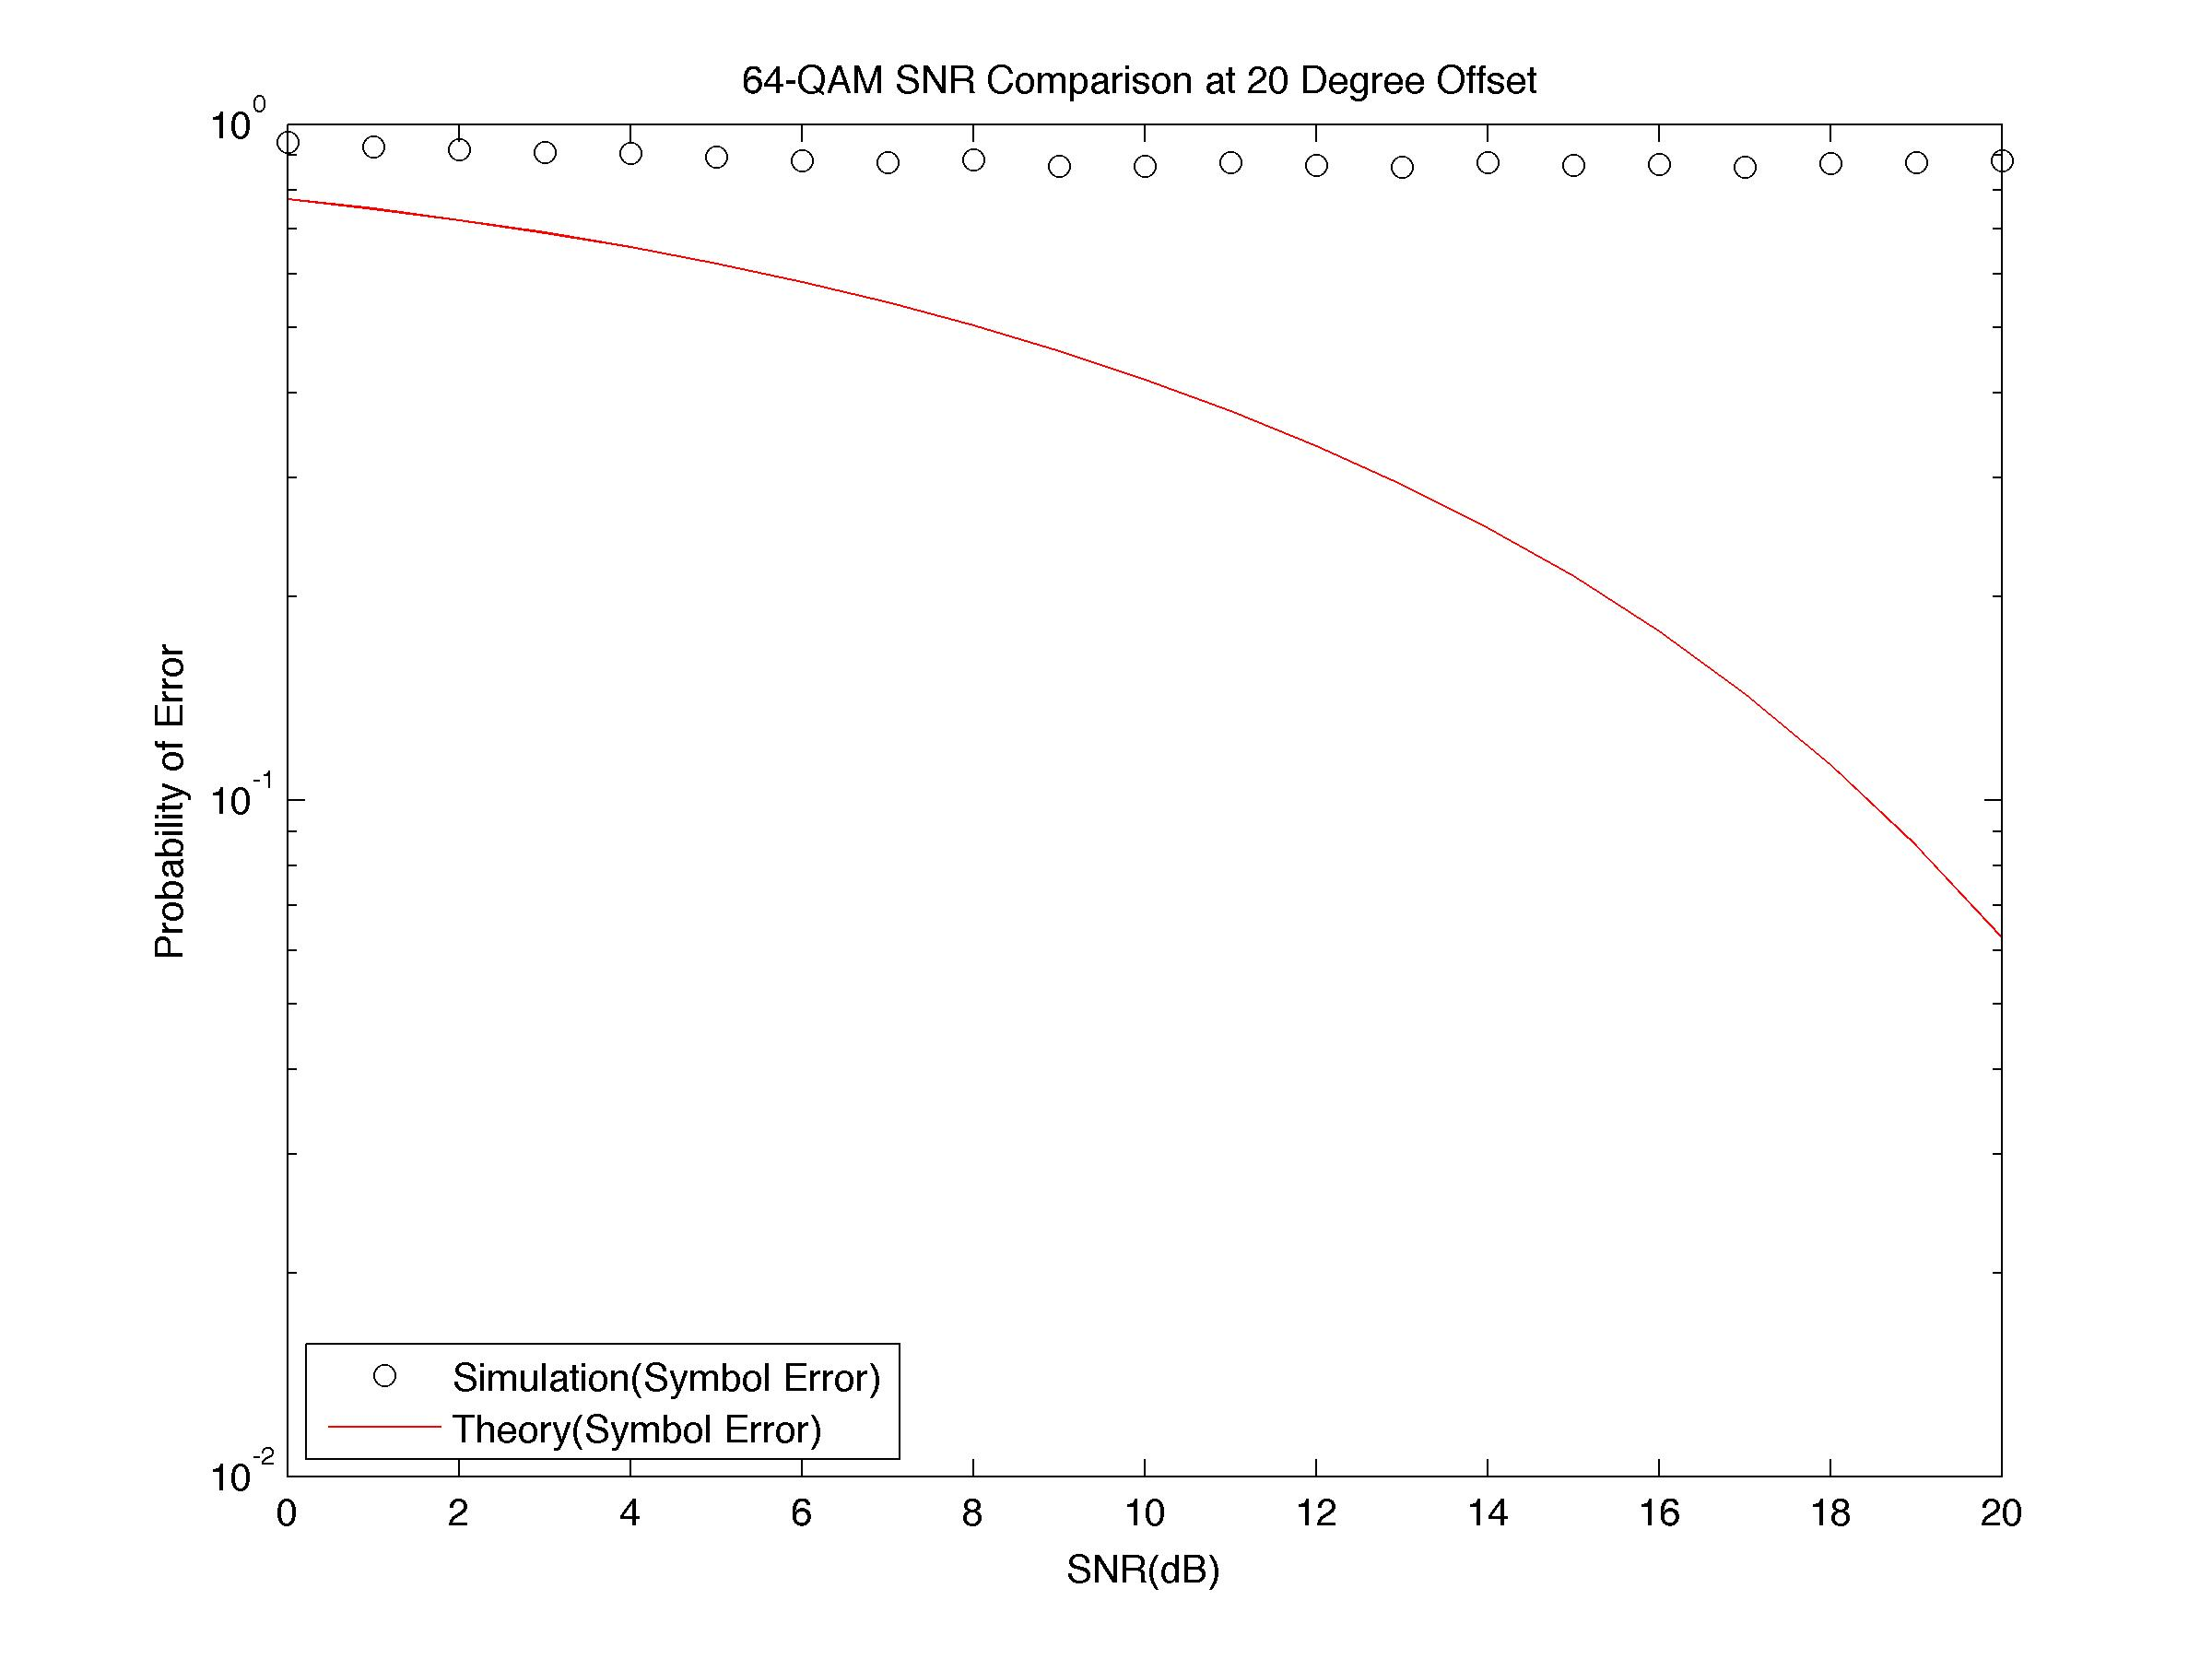
\includegraphics[width=1.3\textwidth]{qam64SNRpo3.jpg}
\caption{64-QAM Theoretical and Experimental error rates versus different SNR levels at a phase offset of 5 degrees }
\end{figure}

\begin{figure}[H]
\centering
\hspace*{-2cm}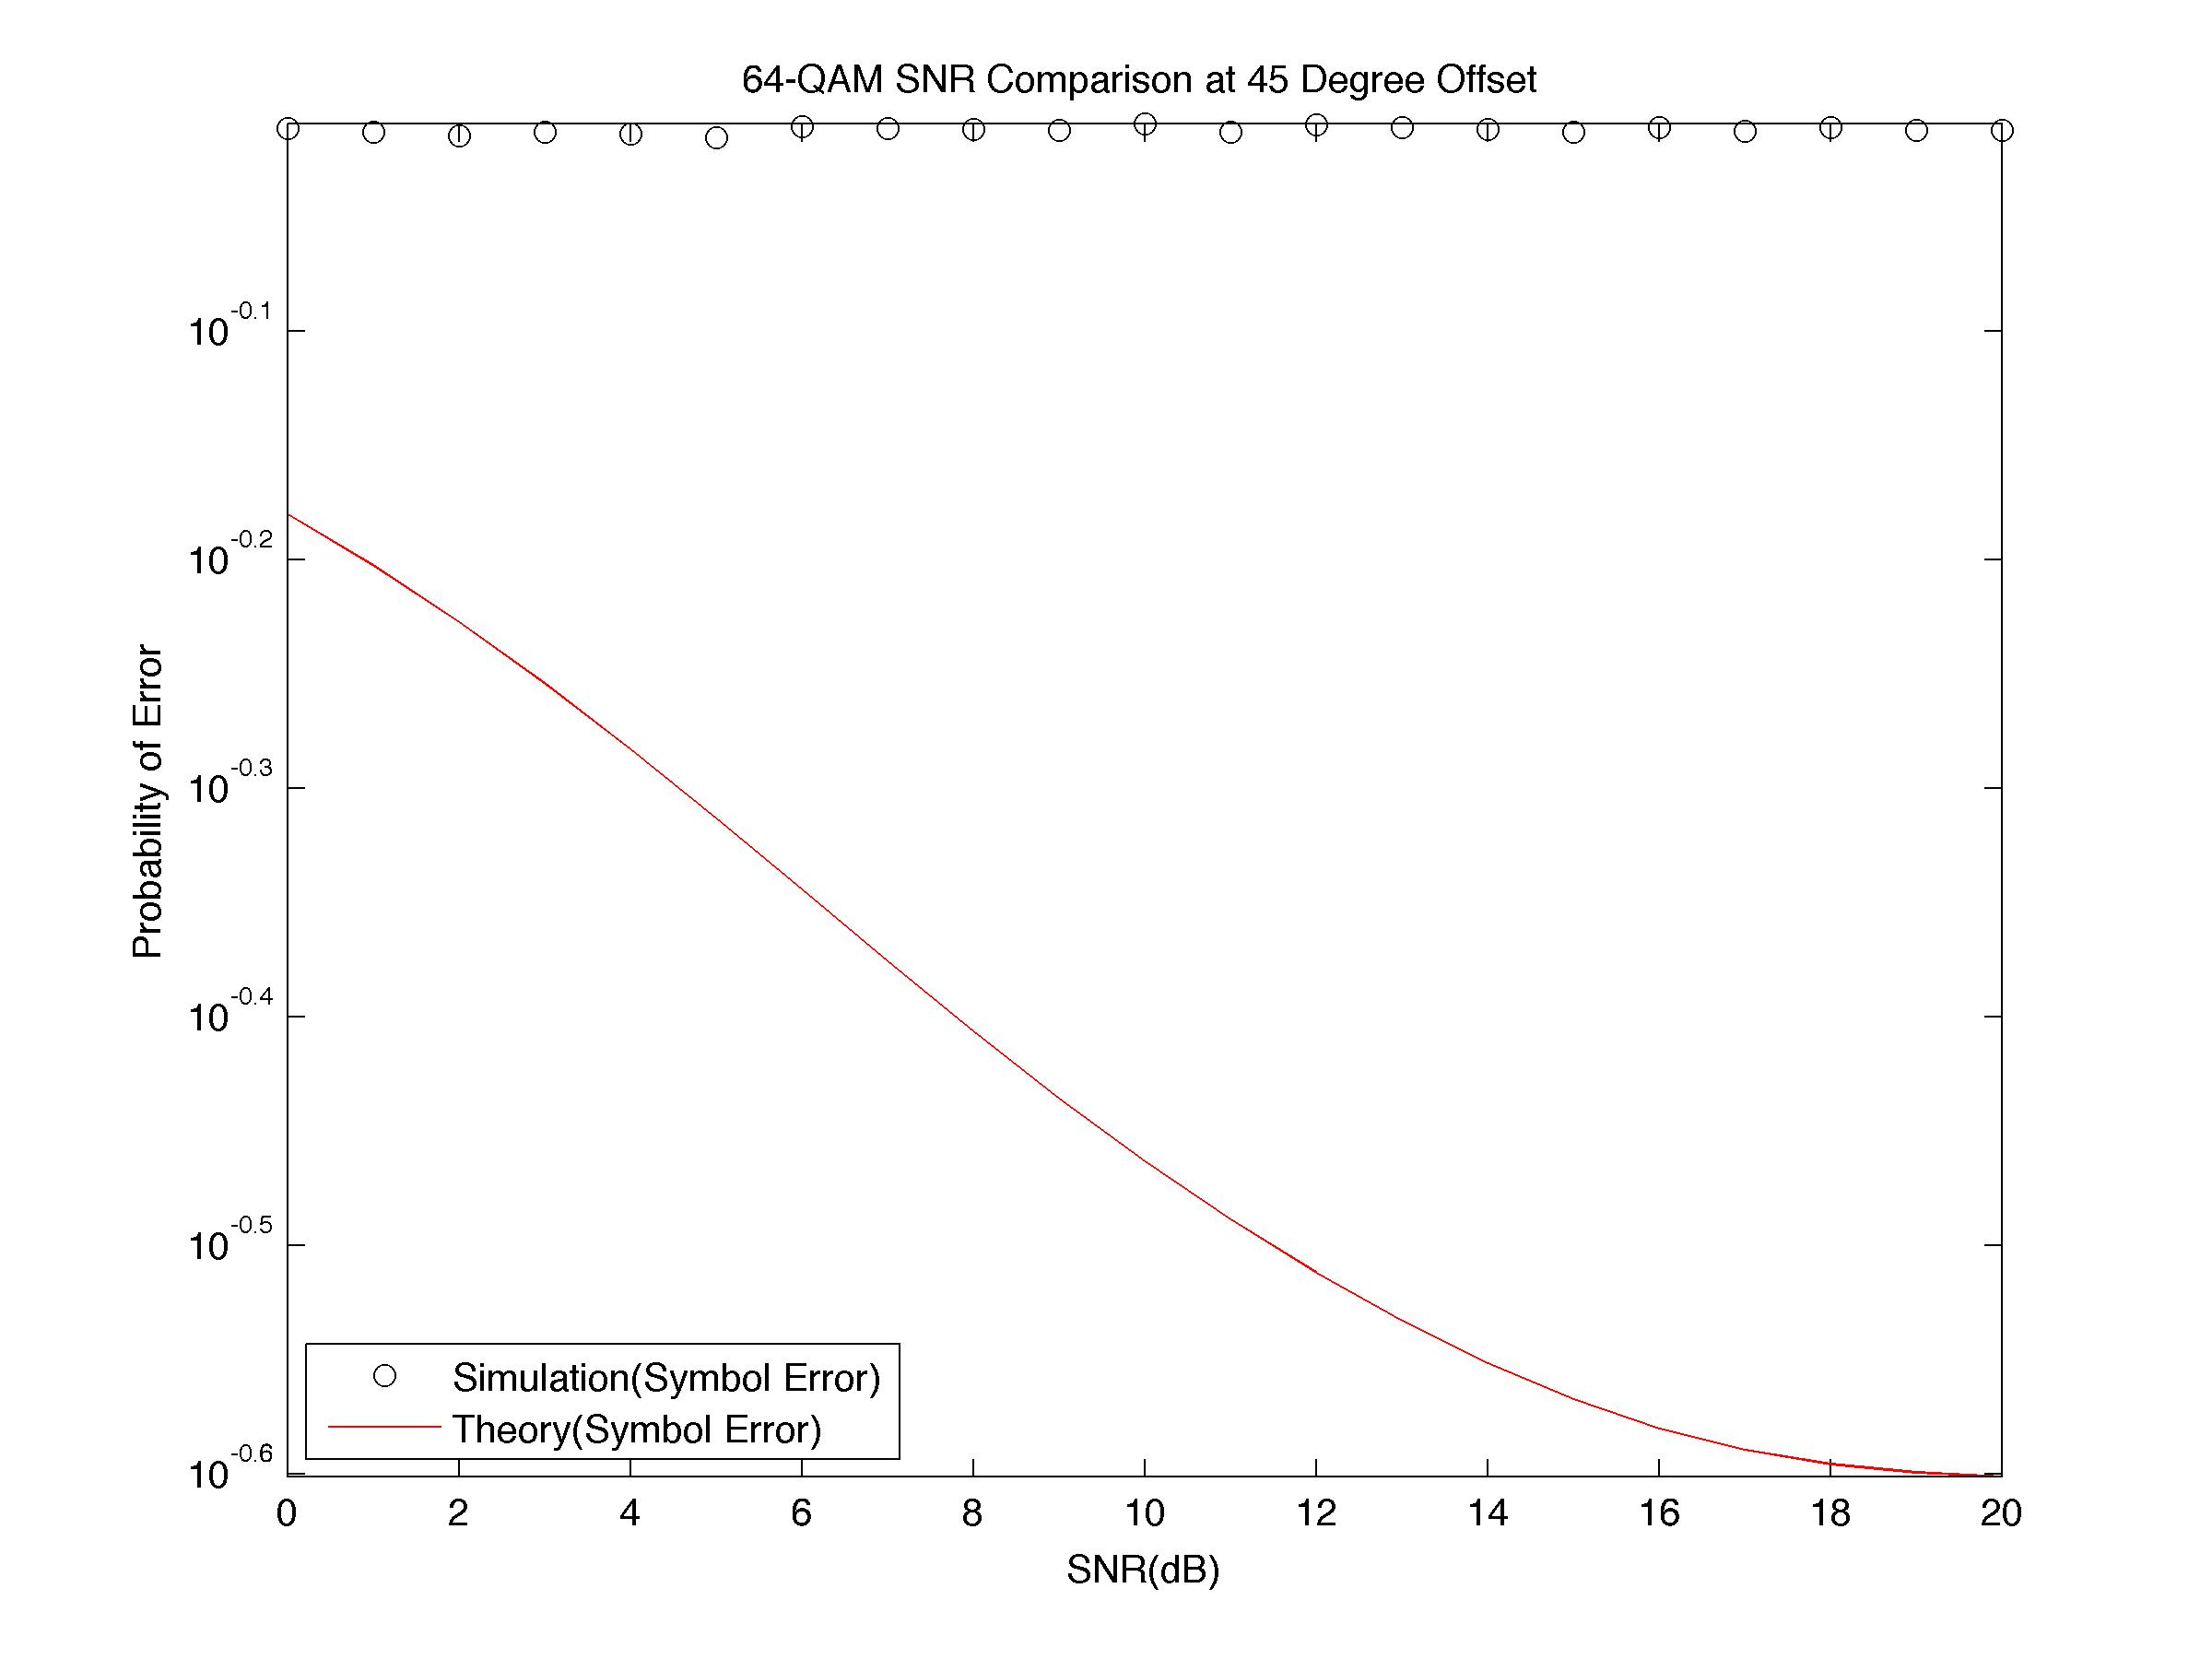
\includegraphics[width=1.3\textwidth]{qam64SNRpo4.jpg}
\caption{64-QAM Theoretical and Experimental error rates versus different SNR levels at a phase offset of 10 degrees }
\end{figure}

\subsection{Constellation Plots for 16-QAM with Phase Offset}
\label{sec:qam16_phaseConst}
In the following sections scatter plots of  16-QAM constellation are plotted at symbol/input SNRs of 3 dB, 6dB, 10dB, 20dB and a phase offsets of 5 degree, 10 degree, 20 degree, 45 degree .

\begin{figure}[H]
\centering
\hspace*{-2cm}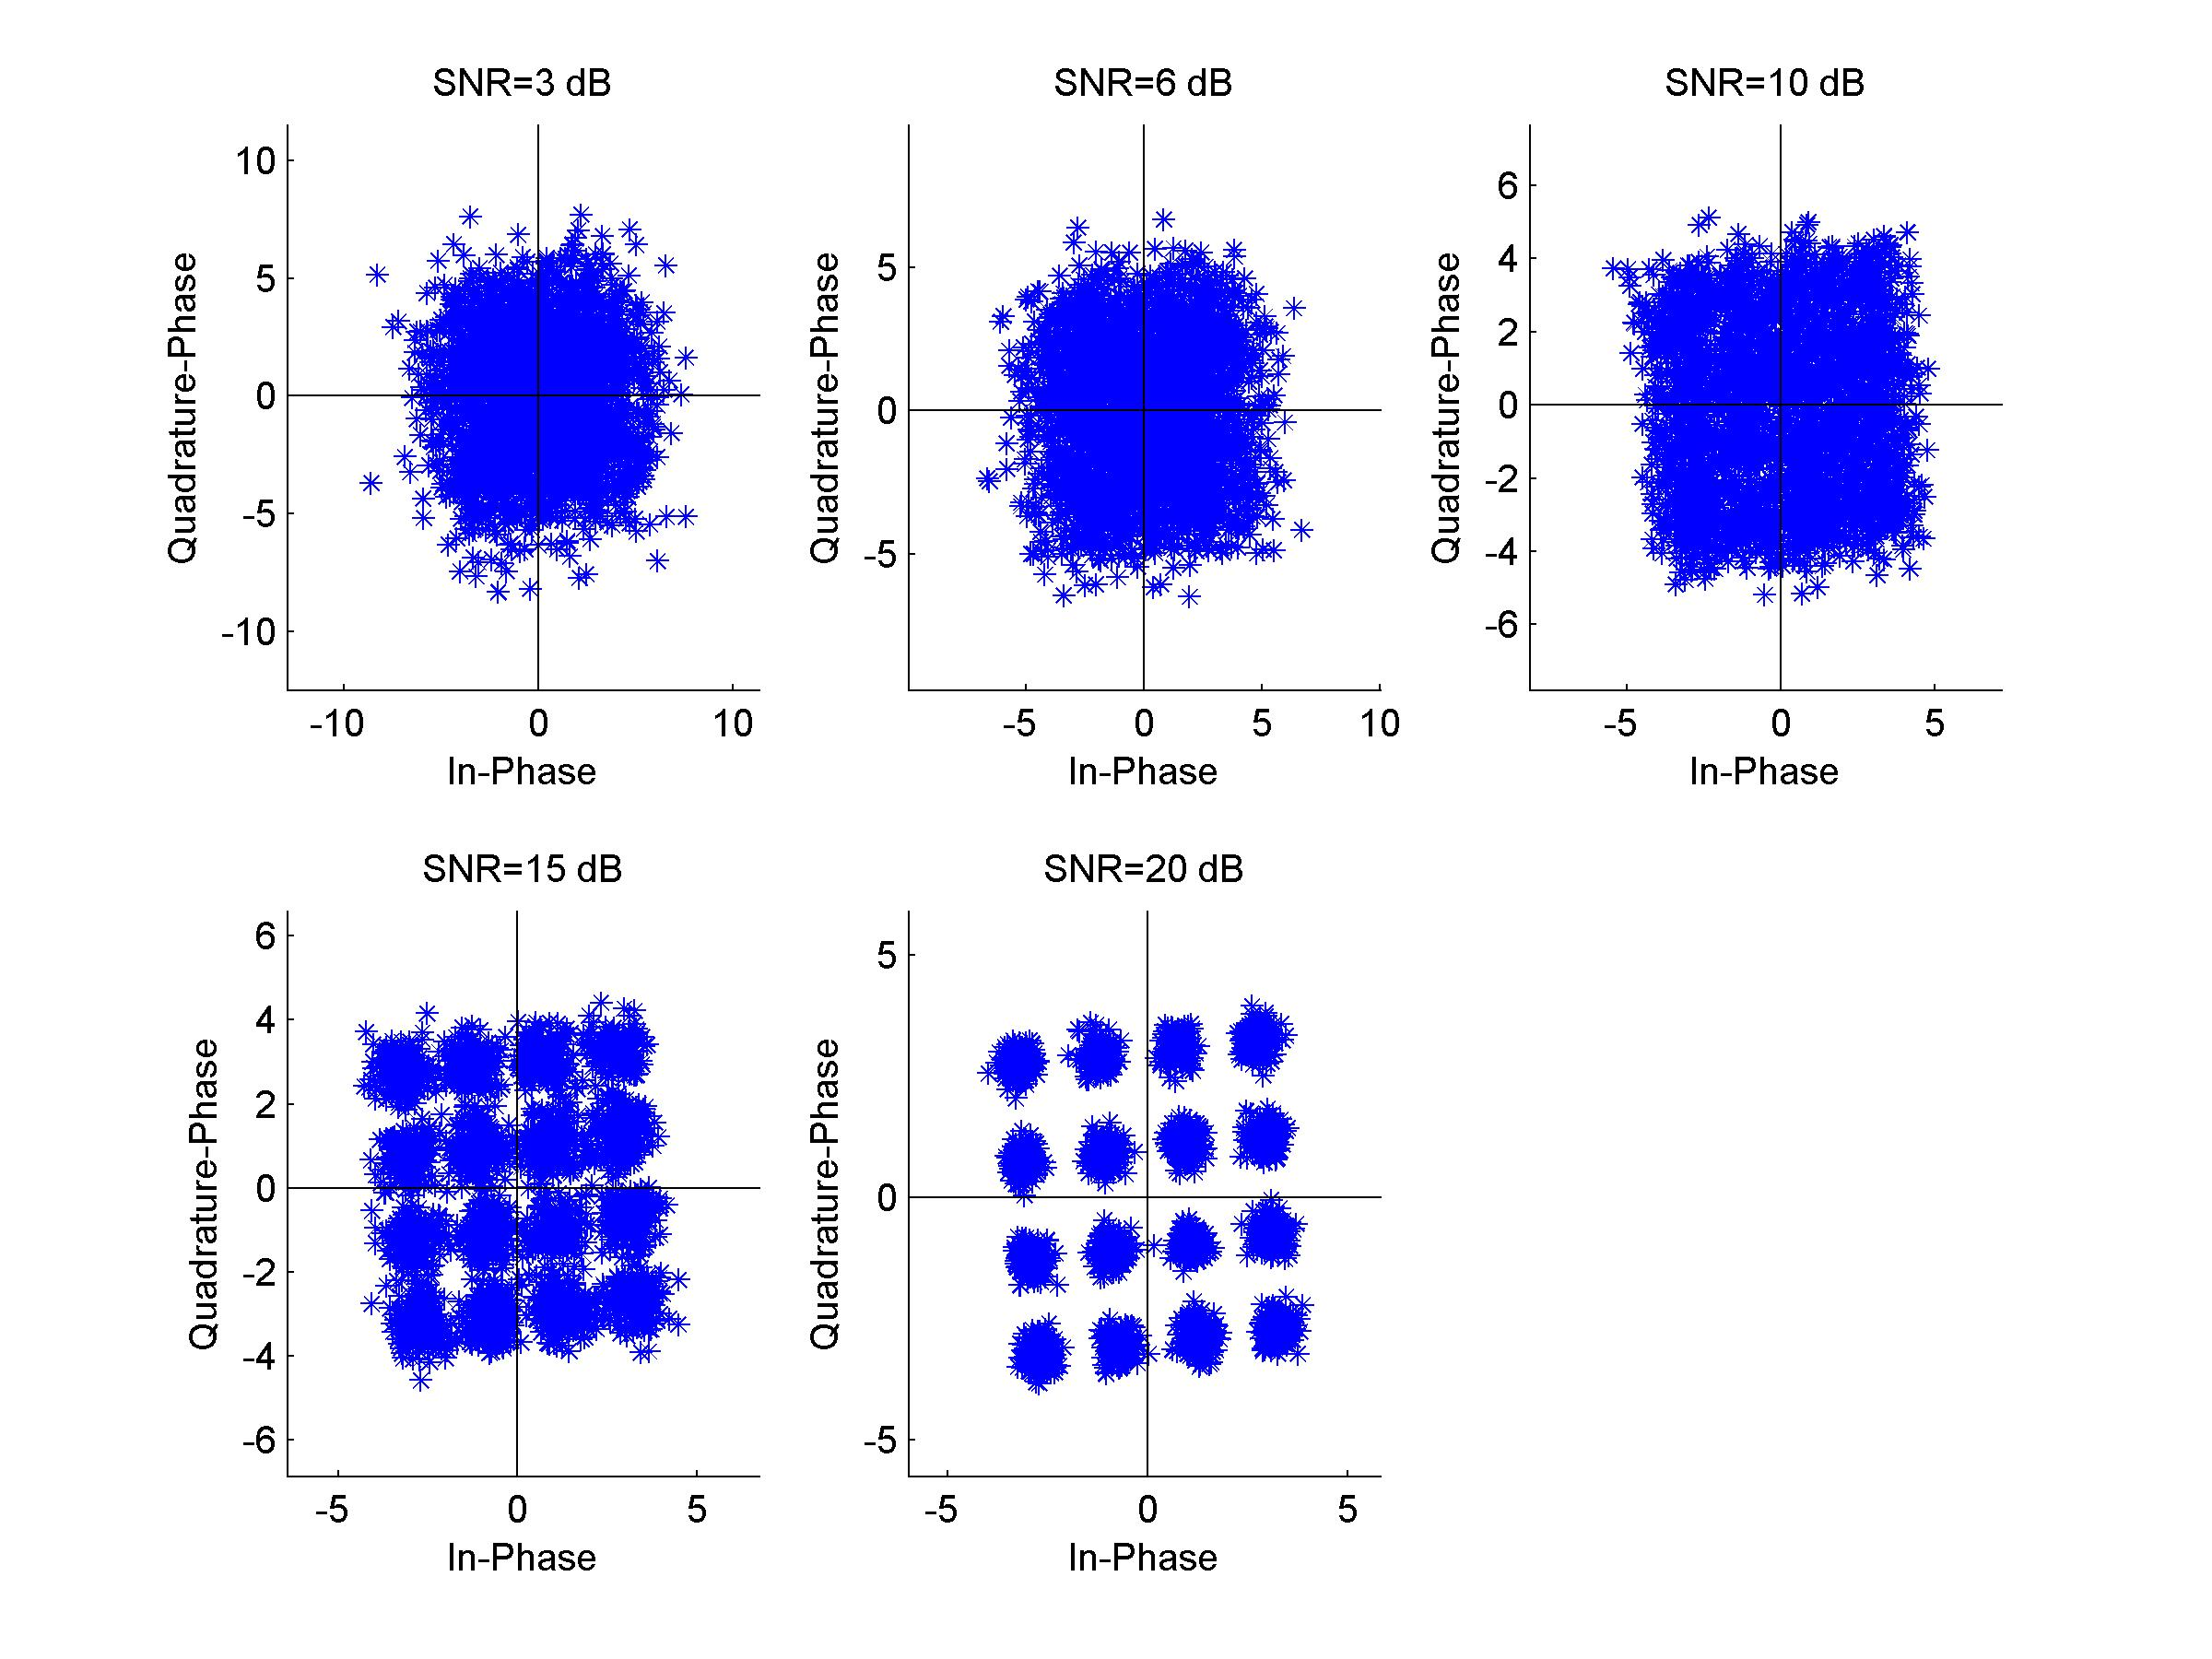
\includegraphics[width=1.3\textwidth]{qam16Constpo1.jpg}
\caption{The 16-QAM constellation plots for different levels of SNR at a phase offset of 5 degrees}
\end{figure}

\begin{figure}[H]
\centering
\hspace*{-2cm}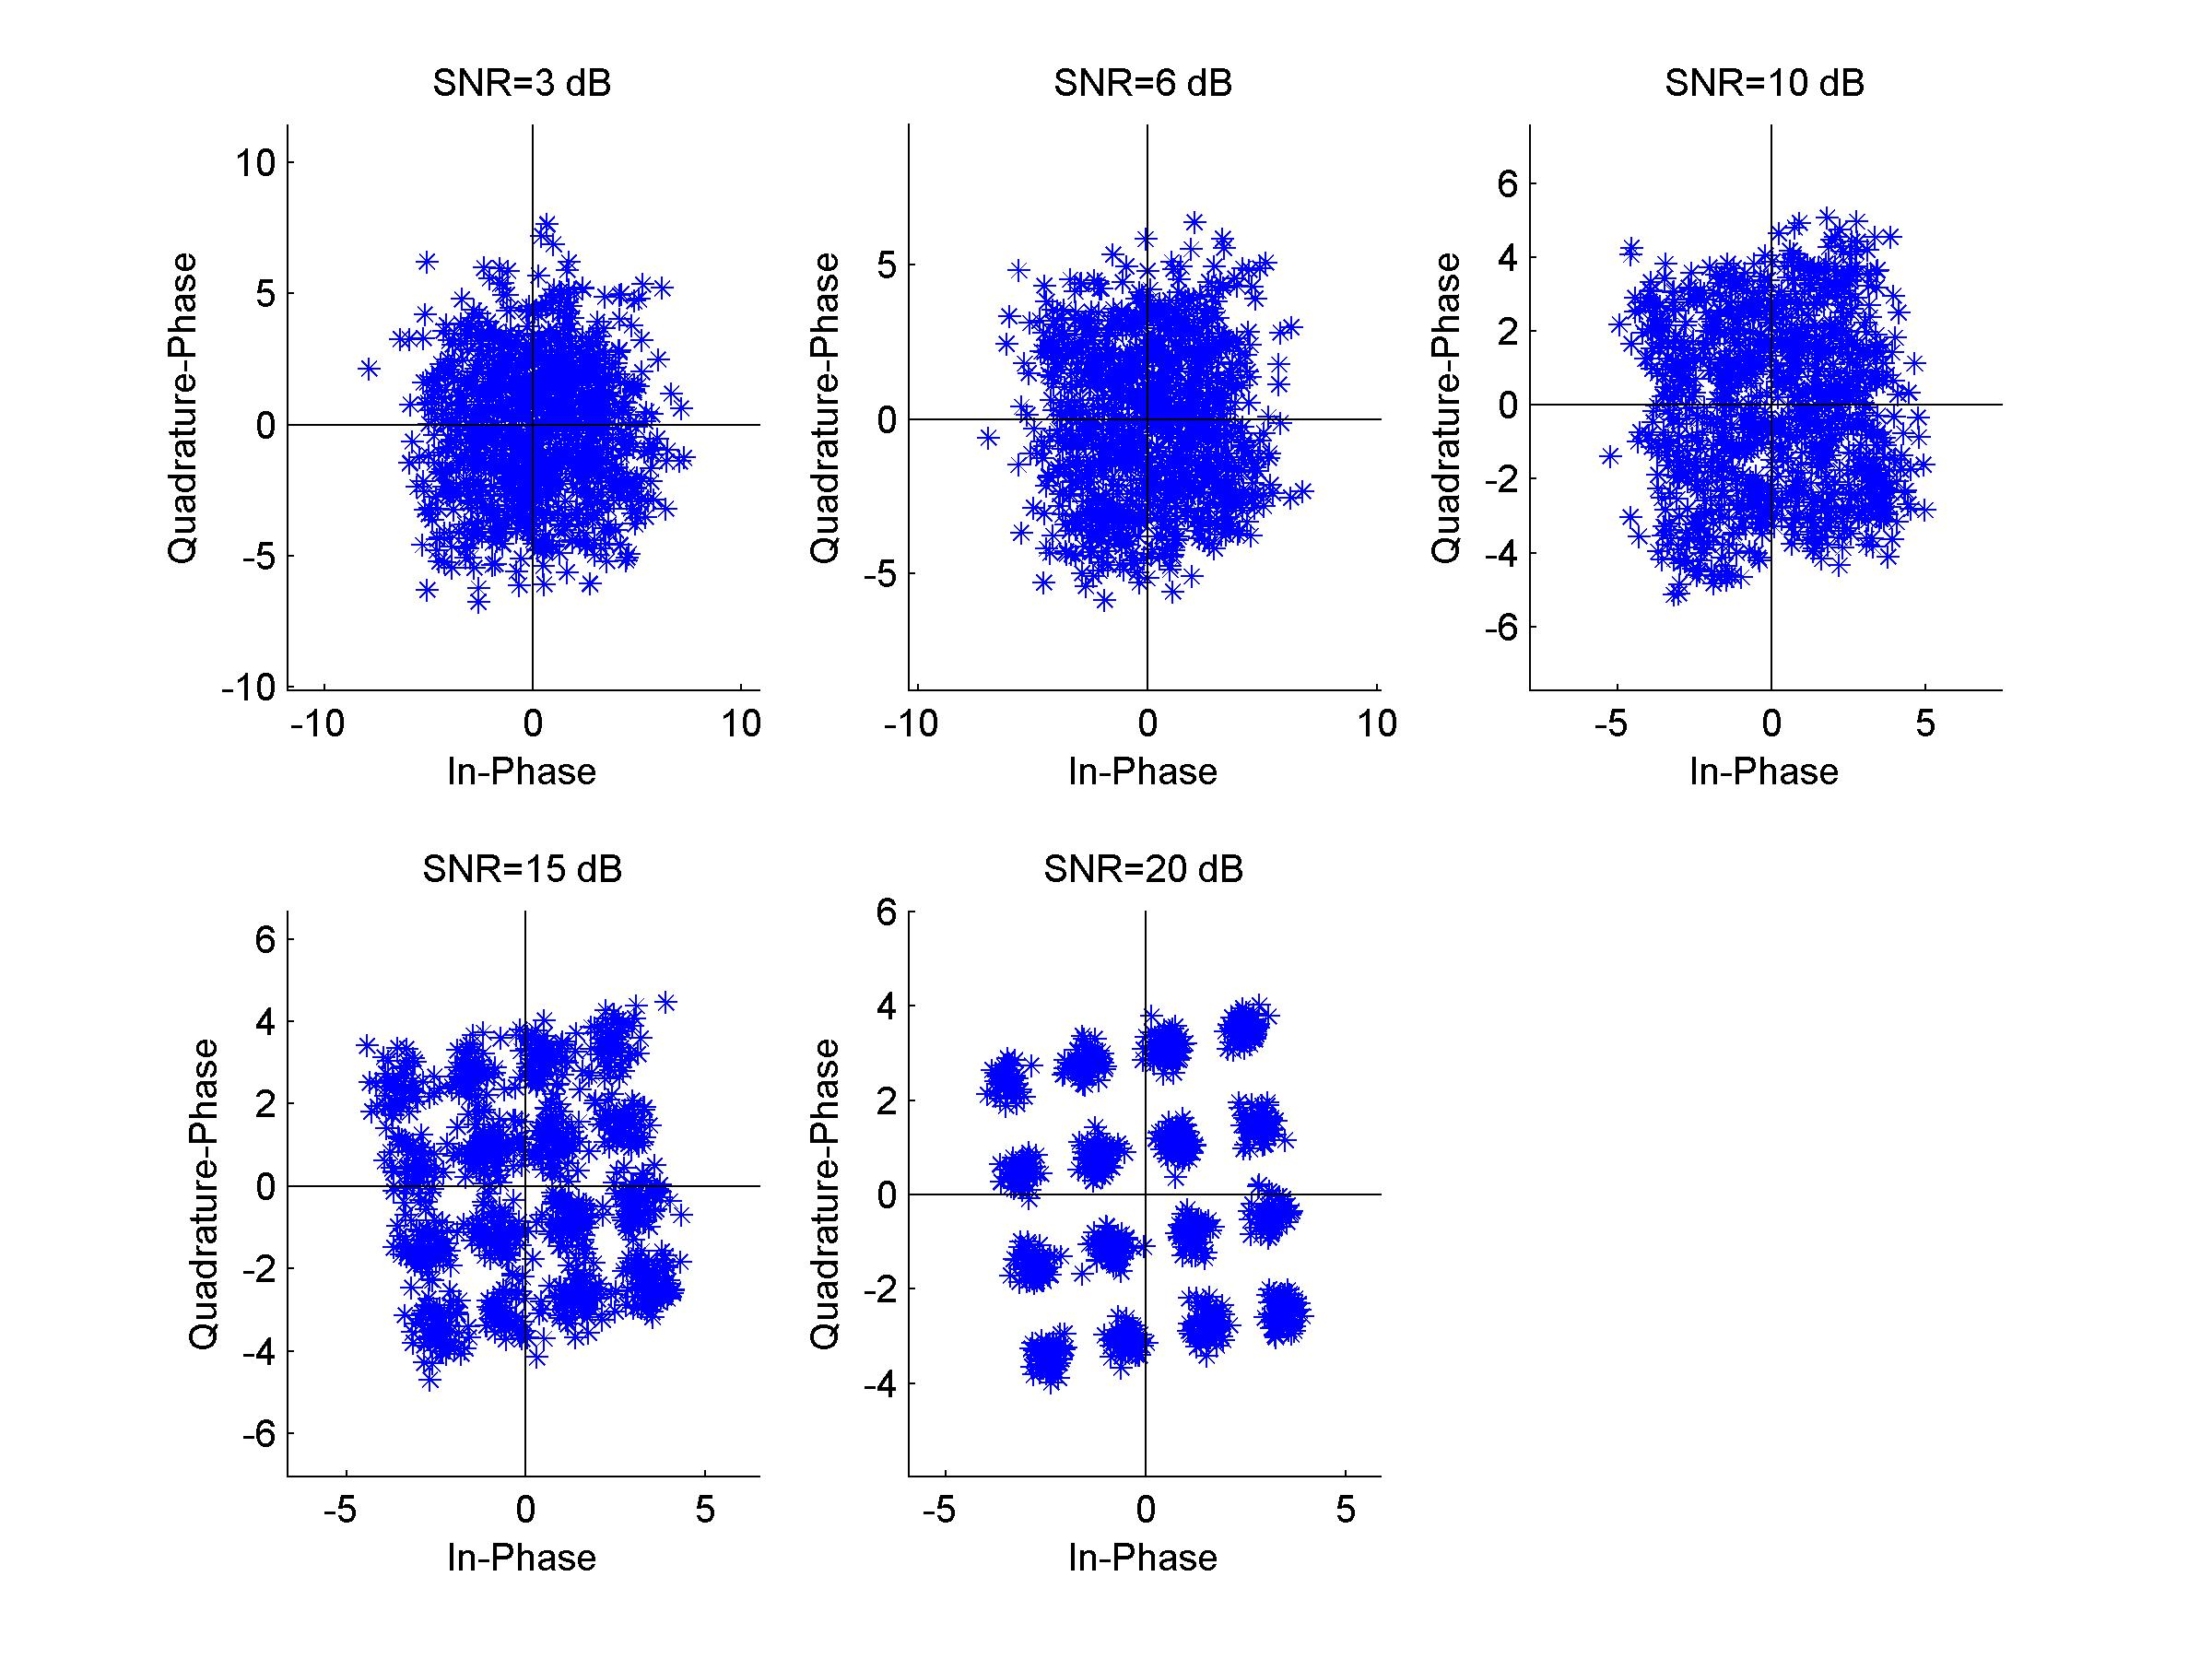
\includegraphics[width=1.3\textwidth]{qam16Constpo2.jpg}
\caption{The 16-QAM constellation plots for different levels of SNR at a phase offset of 10 degrees}
\end{figure}

\begin{figure}[H]
\centering
\hspace*{-2cm}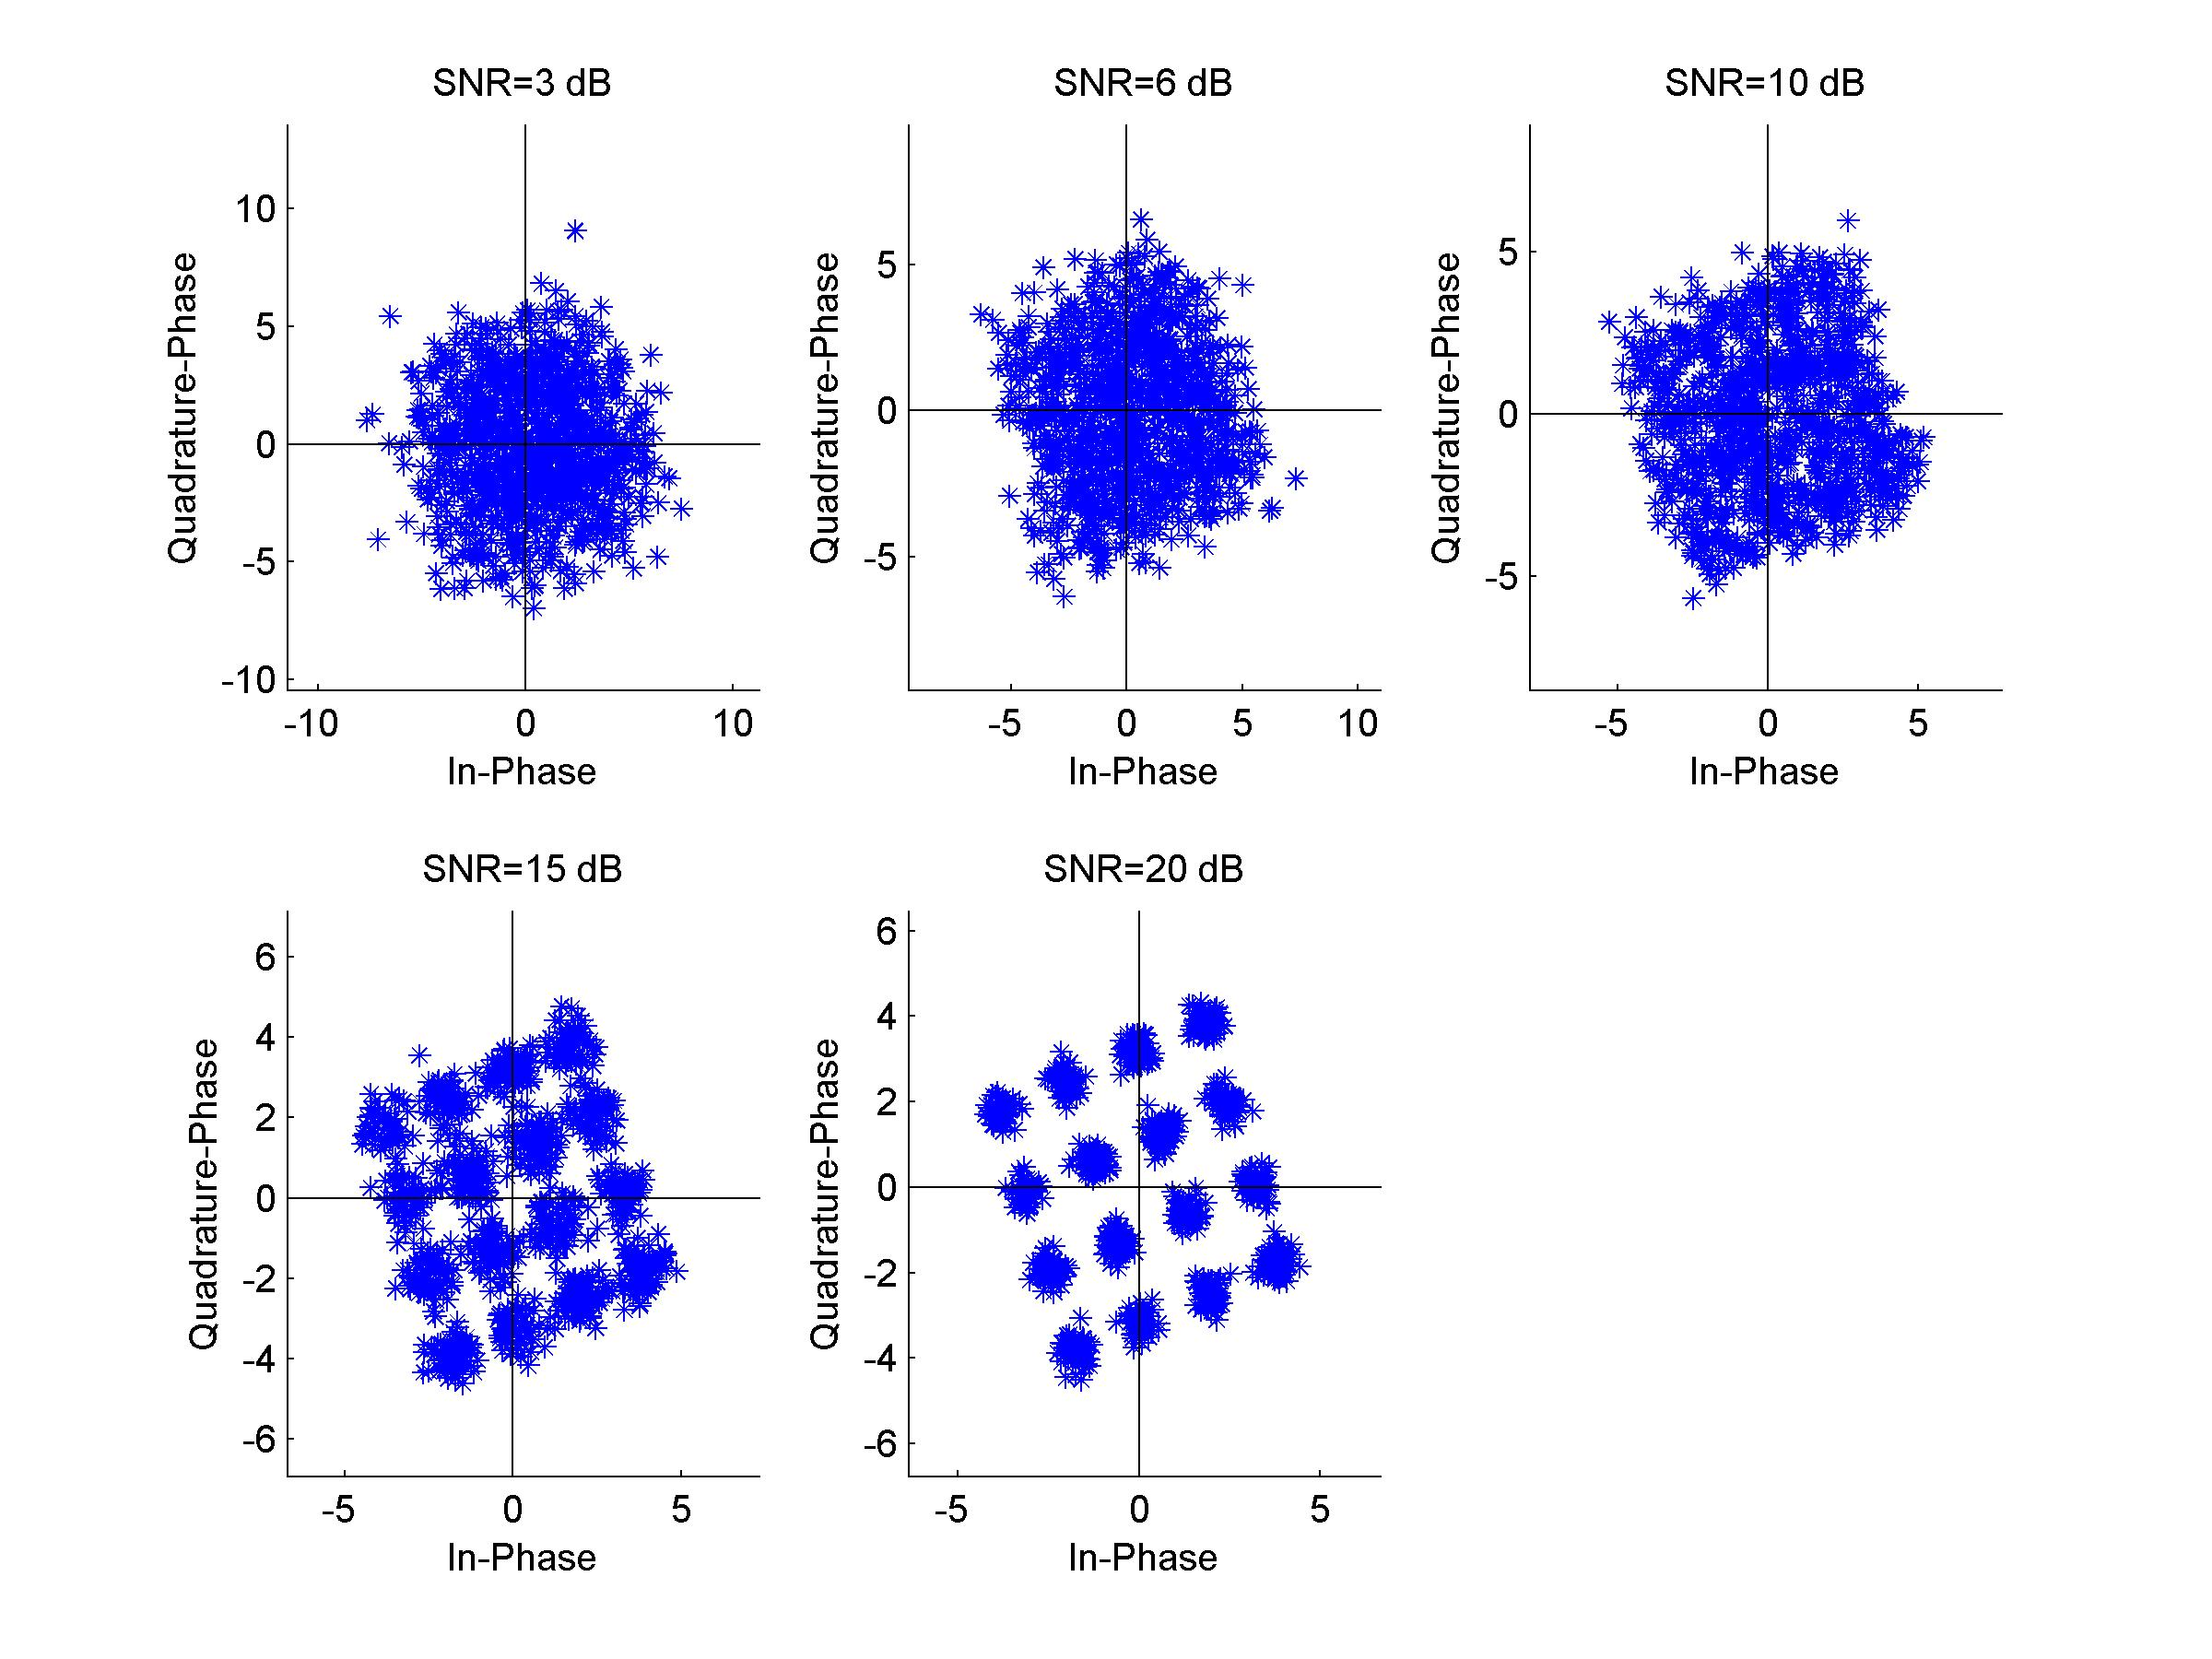
\includegraphics[width=1.3\textwidth]{qam16Constpo3.jpg}
\caption{The 16-QAM constellation plots for different levels of SNR at a phase offset of 20 degrees}
\end{figure}

\begin{figure}[H]
\centering
\hspace*{-2cm}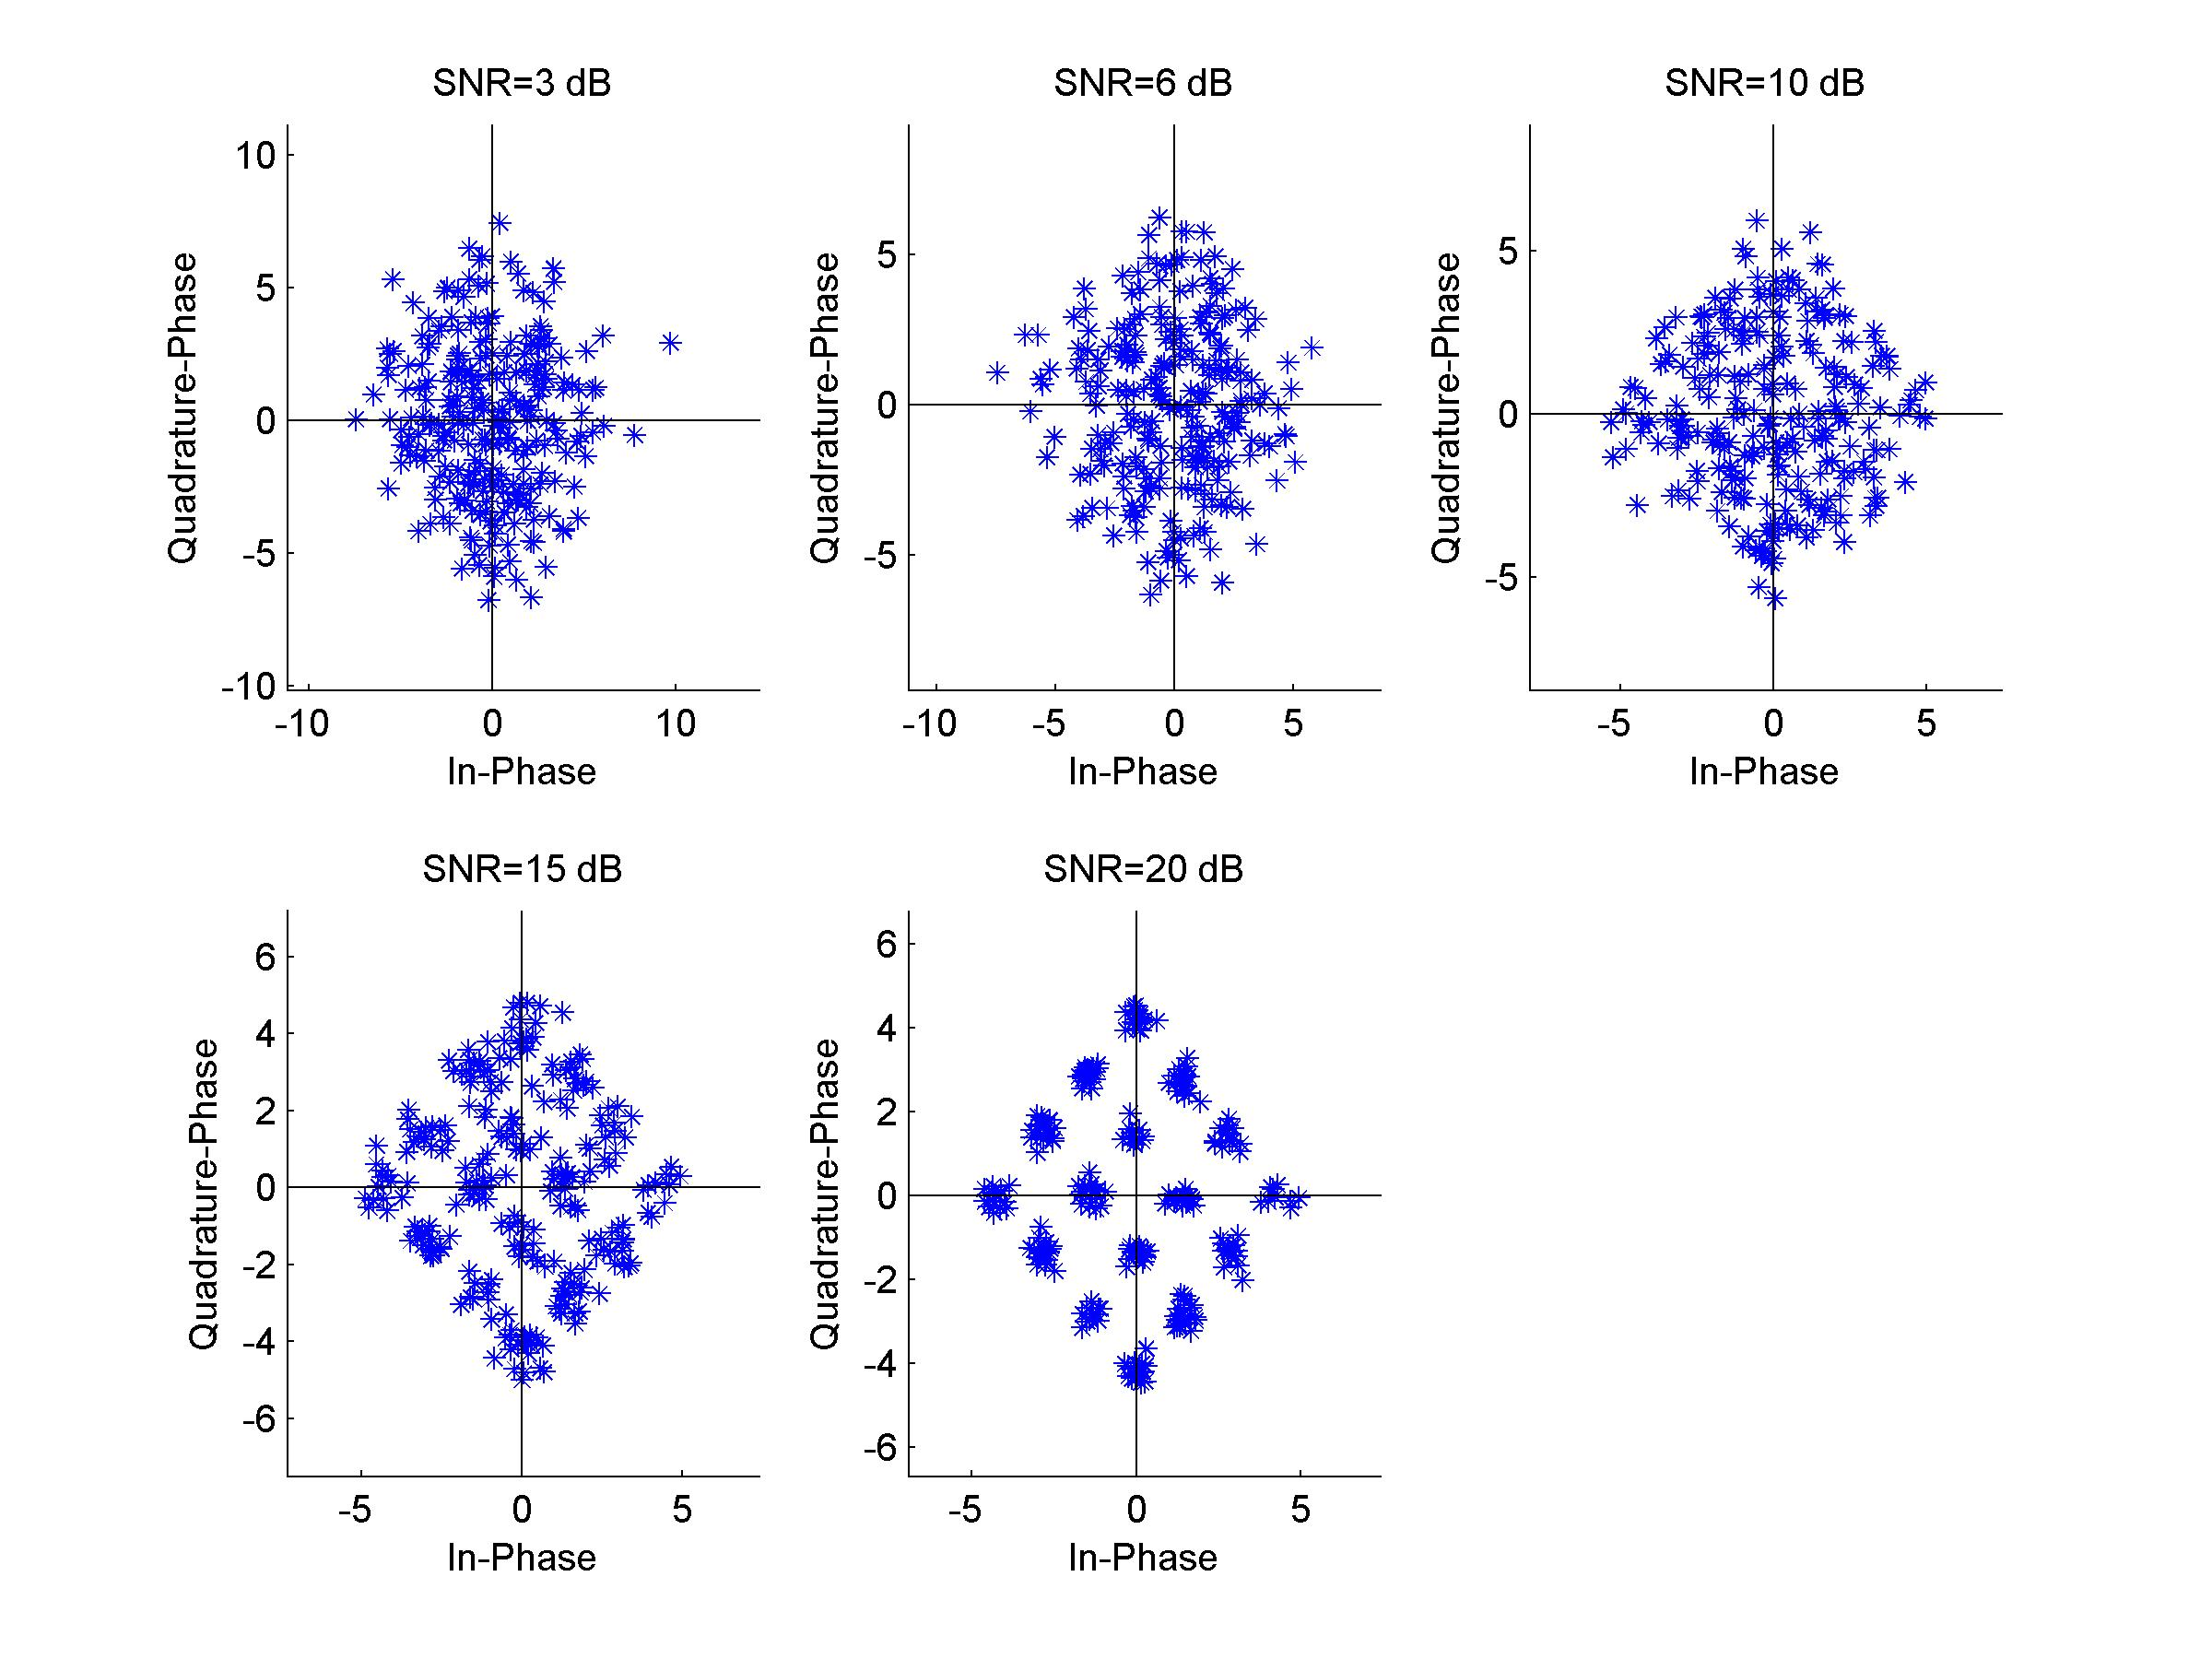
\includegraphics[width=1.3\textwidth]{qam16Constpo4.jpg}
\caption{The 16-QAM constellation plots for different levels of SNR at a phase offset of 45 degrees}
\end{figure}

\section{Step 2 Frequency Offset Results}
\label{sec:results_fo}
In the following sections, the probability of bit error versus the signal to noise ratio is shown on scatter plots for BPSK, QPSK, 16-QAM and 64-QAM constellations .

\subsection{Probability of Error vs SNR plots for Constellations with Frequency Offset}
In the sections given below, the constellations of BPSK, QPSK, 16-QAM and 64-QAM are plotted using the MATLAB functions given in the appendix:
\begin{itemize}
\item Theoretical Bit Error Rate/Symbol Error Rate curve as a function of the symbol SNR
\item The theoretical Bit Error Rate/Symbol Error Rate curve as a function of $E_b/N_o$
\item The Bit Error Rate/Symbol Error Rate curve from the simulation as a function of the received signal's SNR
\end{itemize}

\subsubsection{BPSK with Frequency Offset}
\begin{figure}[H]
\centering
\hspace*{-2cm}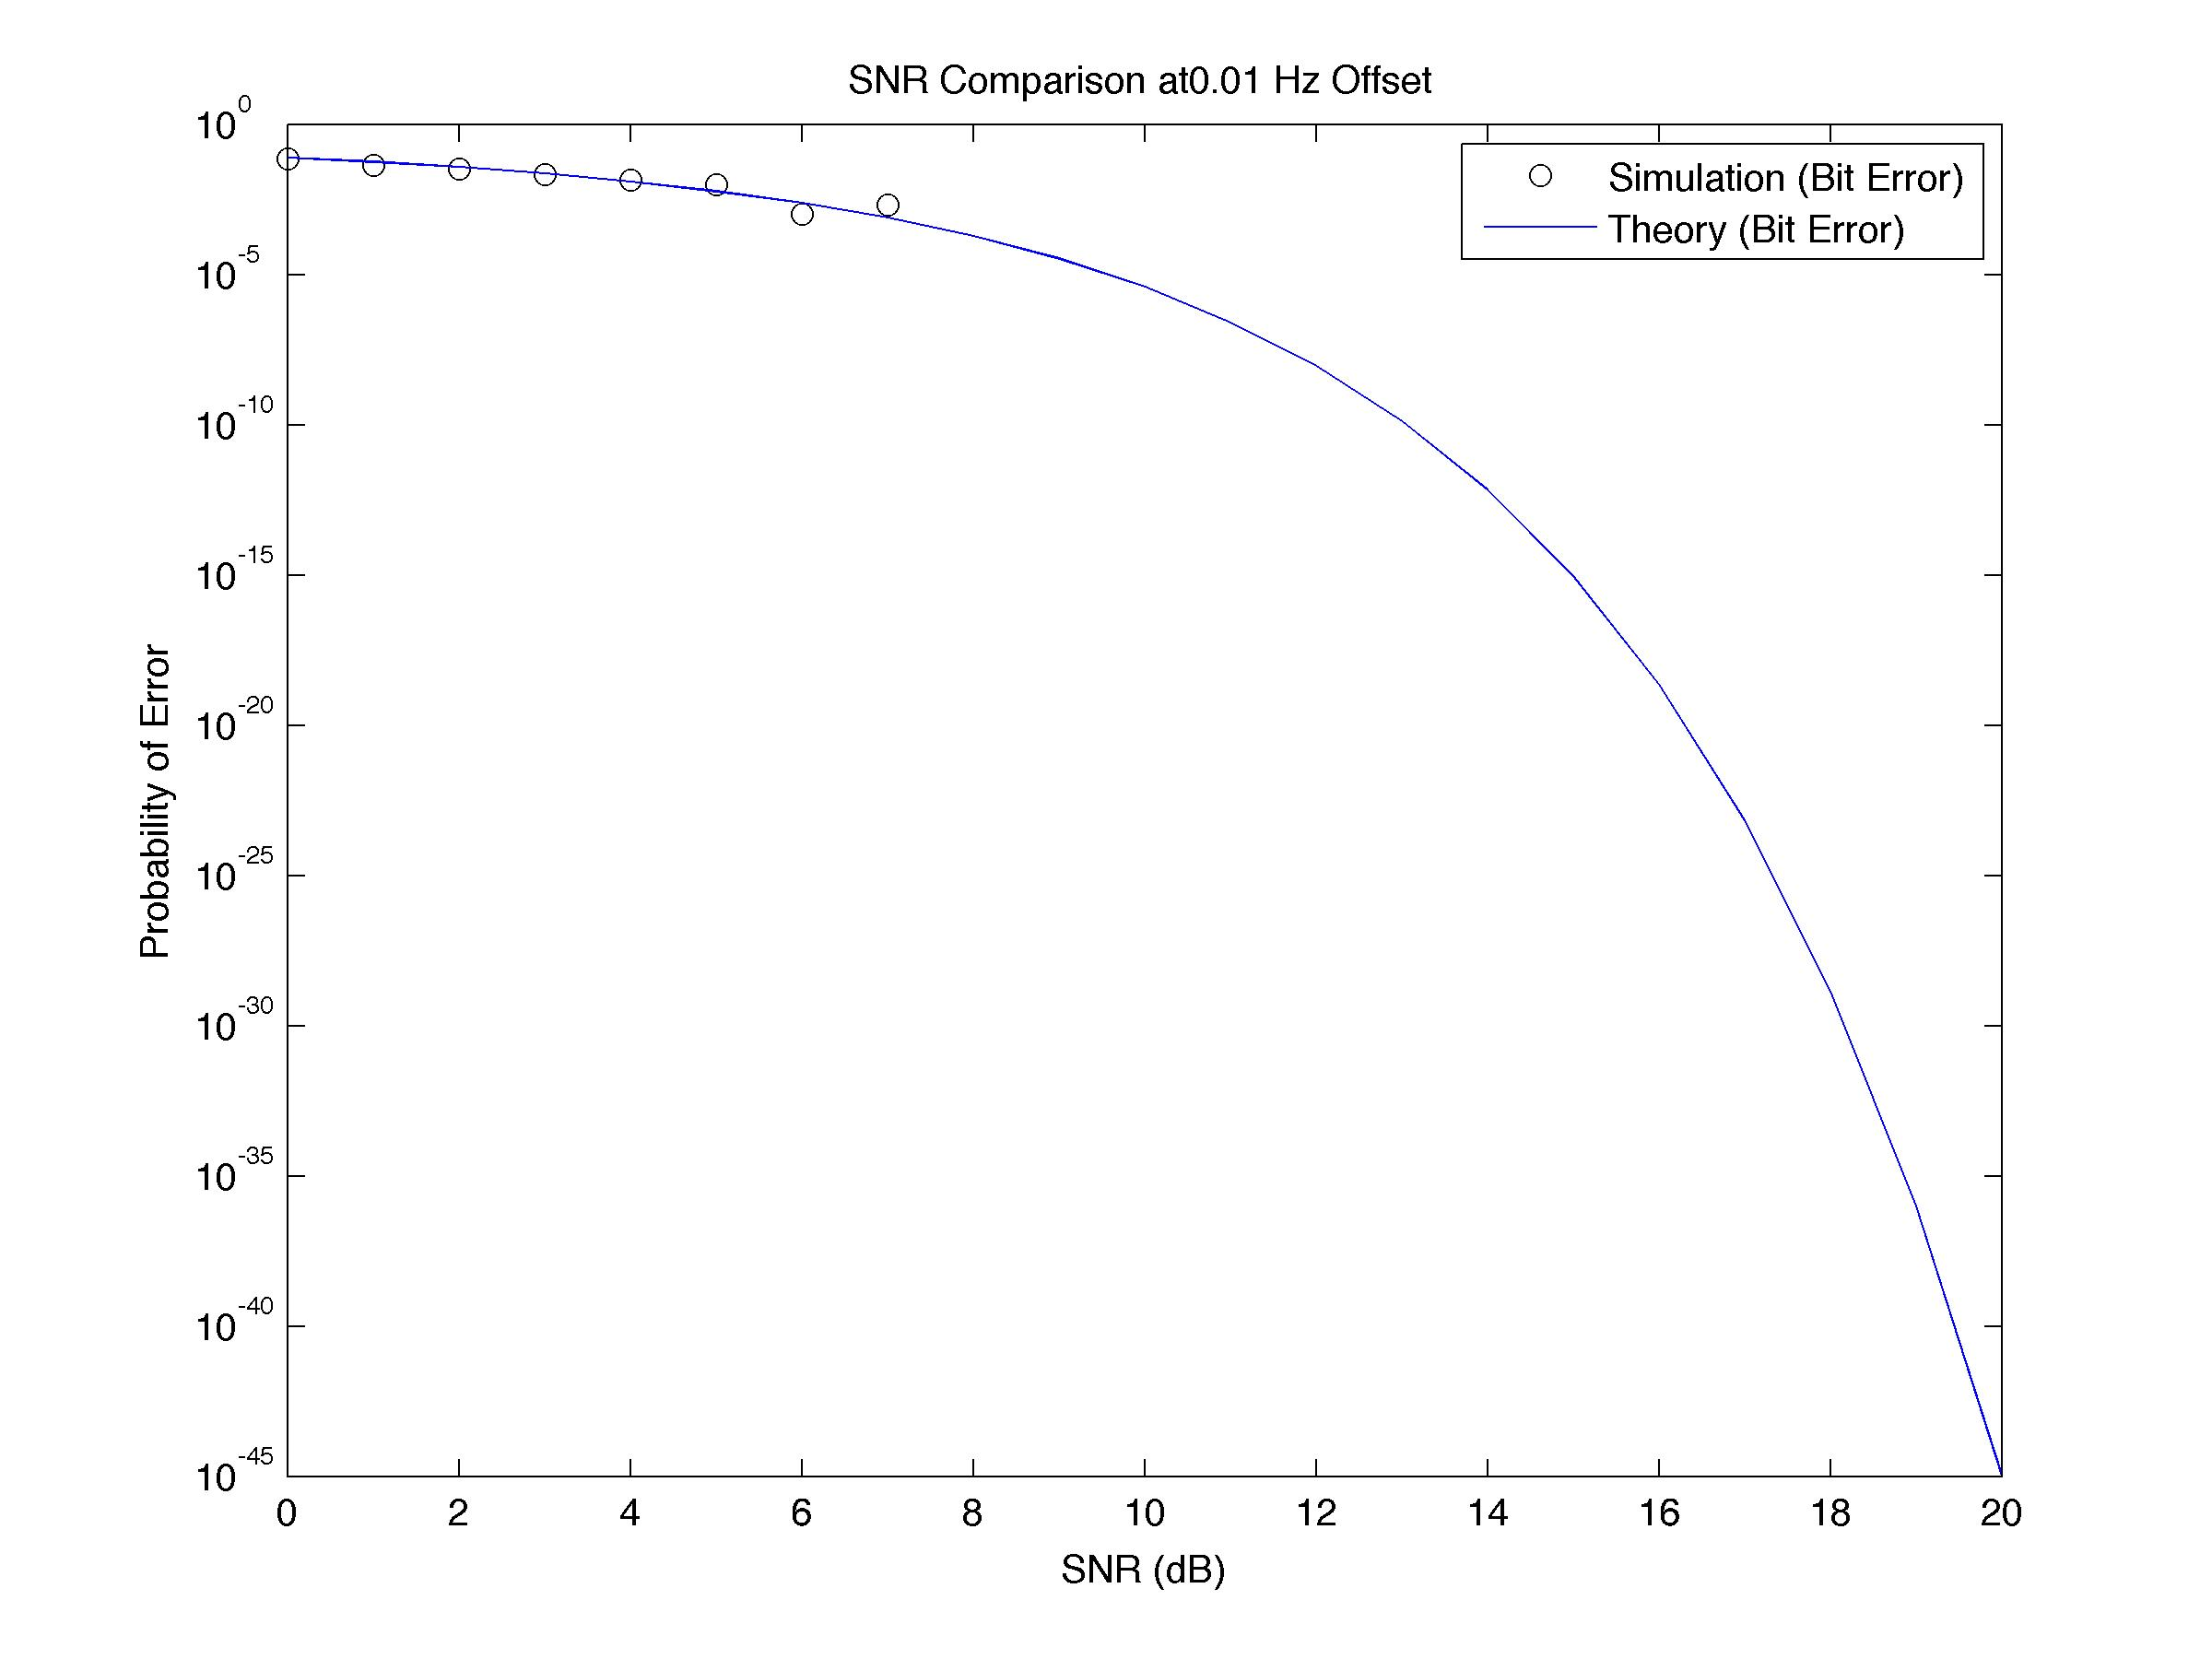
\includegraphics[width=1.3\textwidth]{bpSNRfo1.jpg}
\caption{BPSK Theoretical and Experimental error rates versus different SNR levels at a frequency offset of 0.01 Hz}
\end{figure}

\begin{figure}[H]
\centering
\hspace*{-2cm}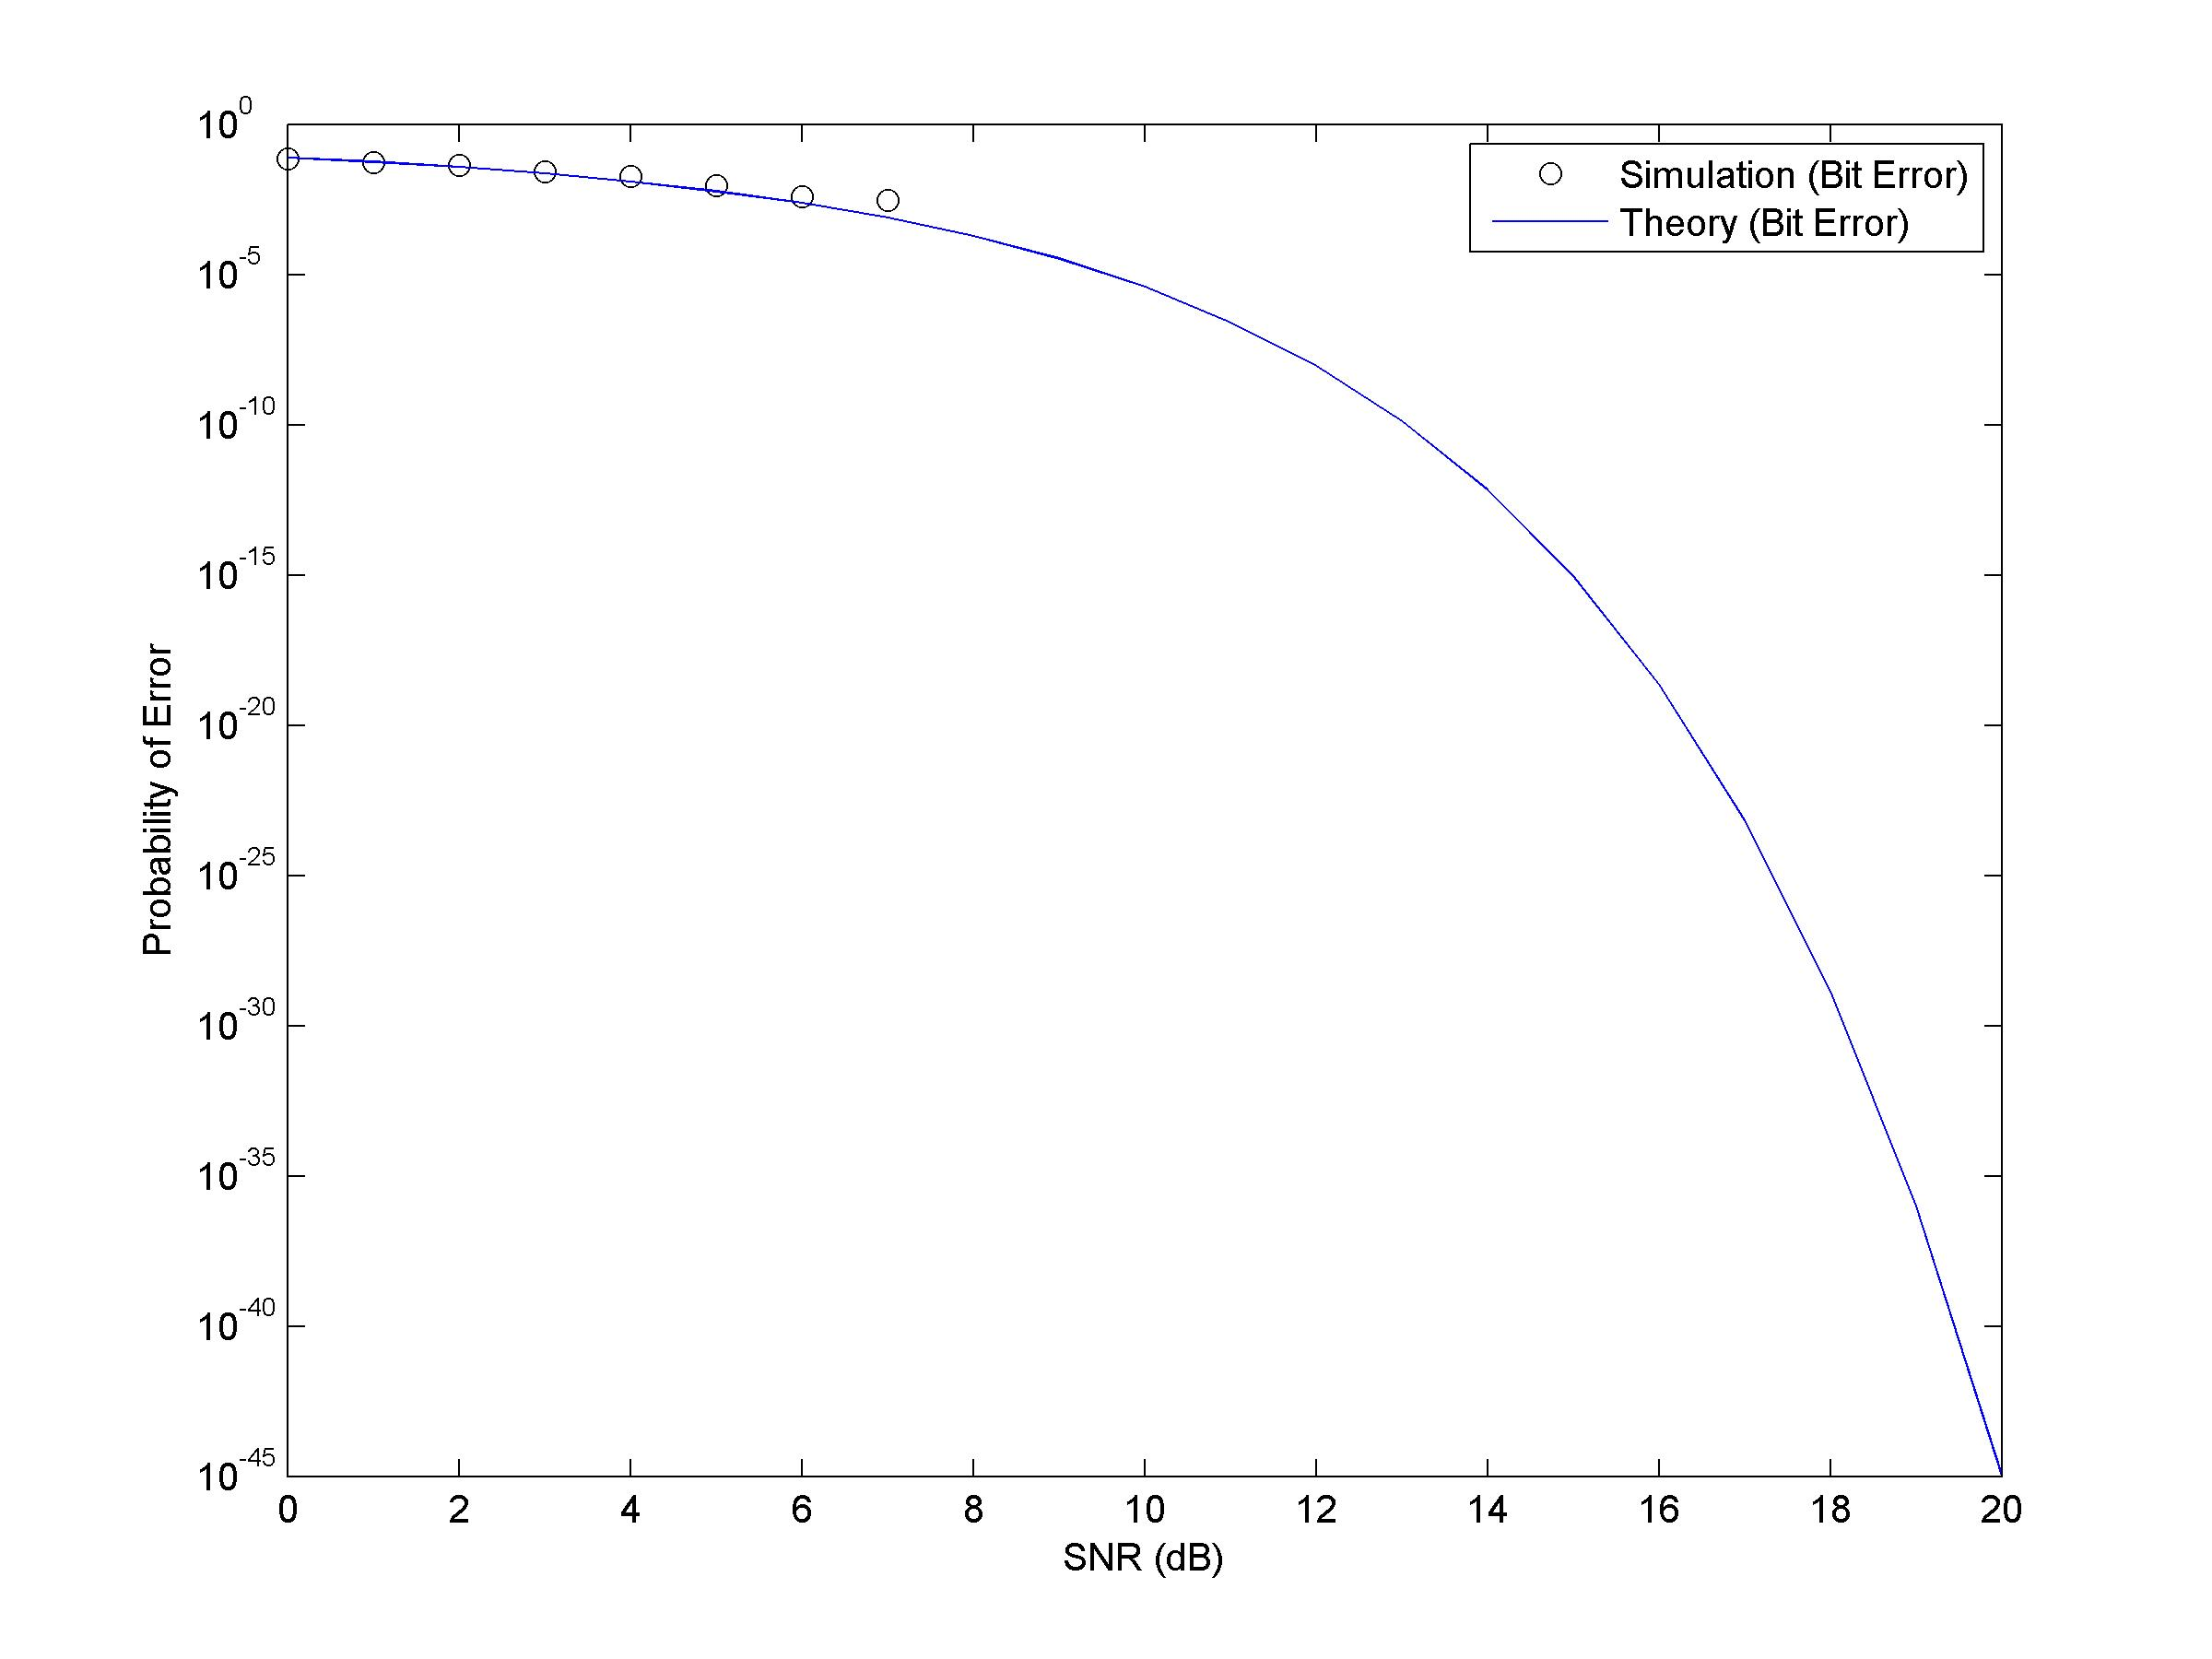
\includegraphics[width=1.3\textwidth]{bpSNRfo2.jpg}
\caption{BPSK Theoretical and Experimental error rates versus different SNR levels at a frequency offset of 0.1 Hz}
\end{figure}


\begin{figure}[H]
\centering
\hspace*{-2cm}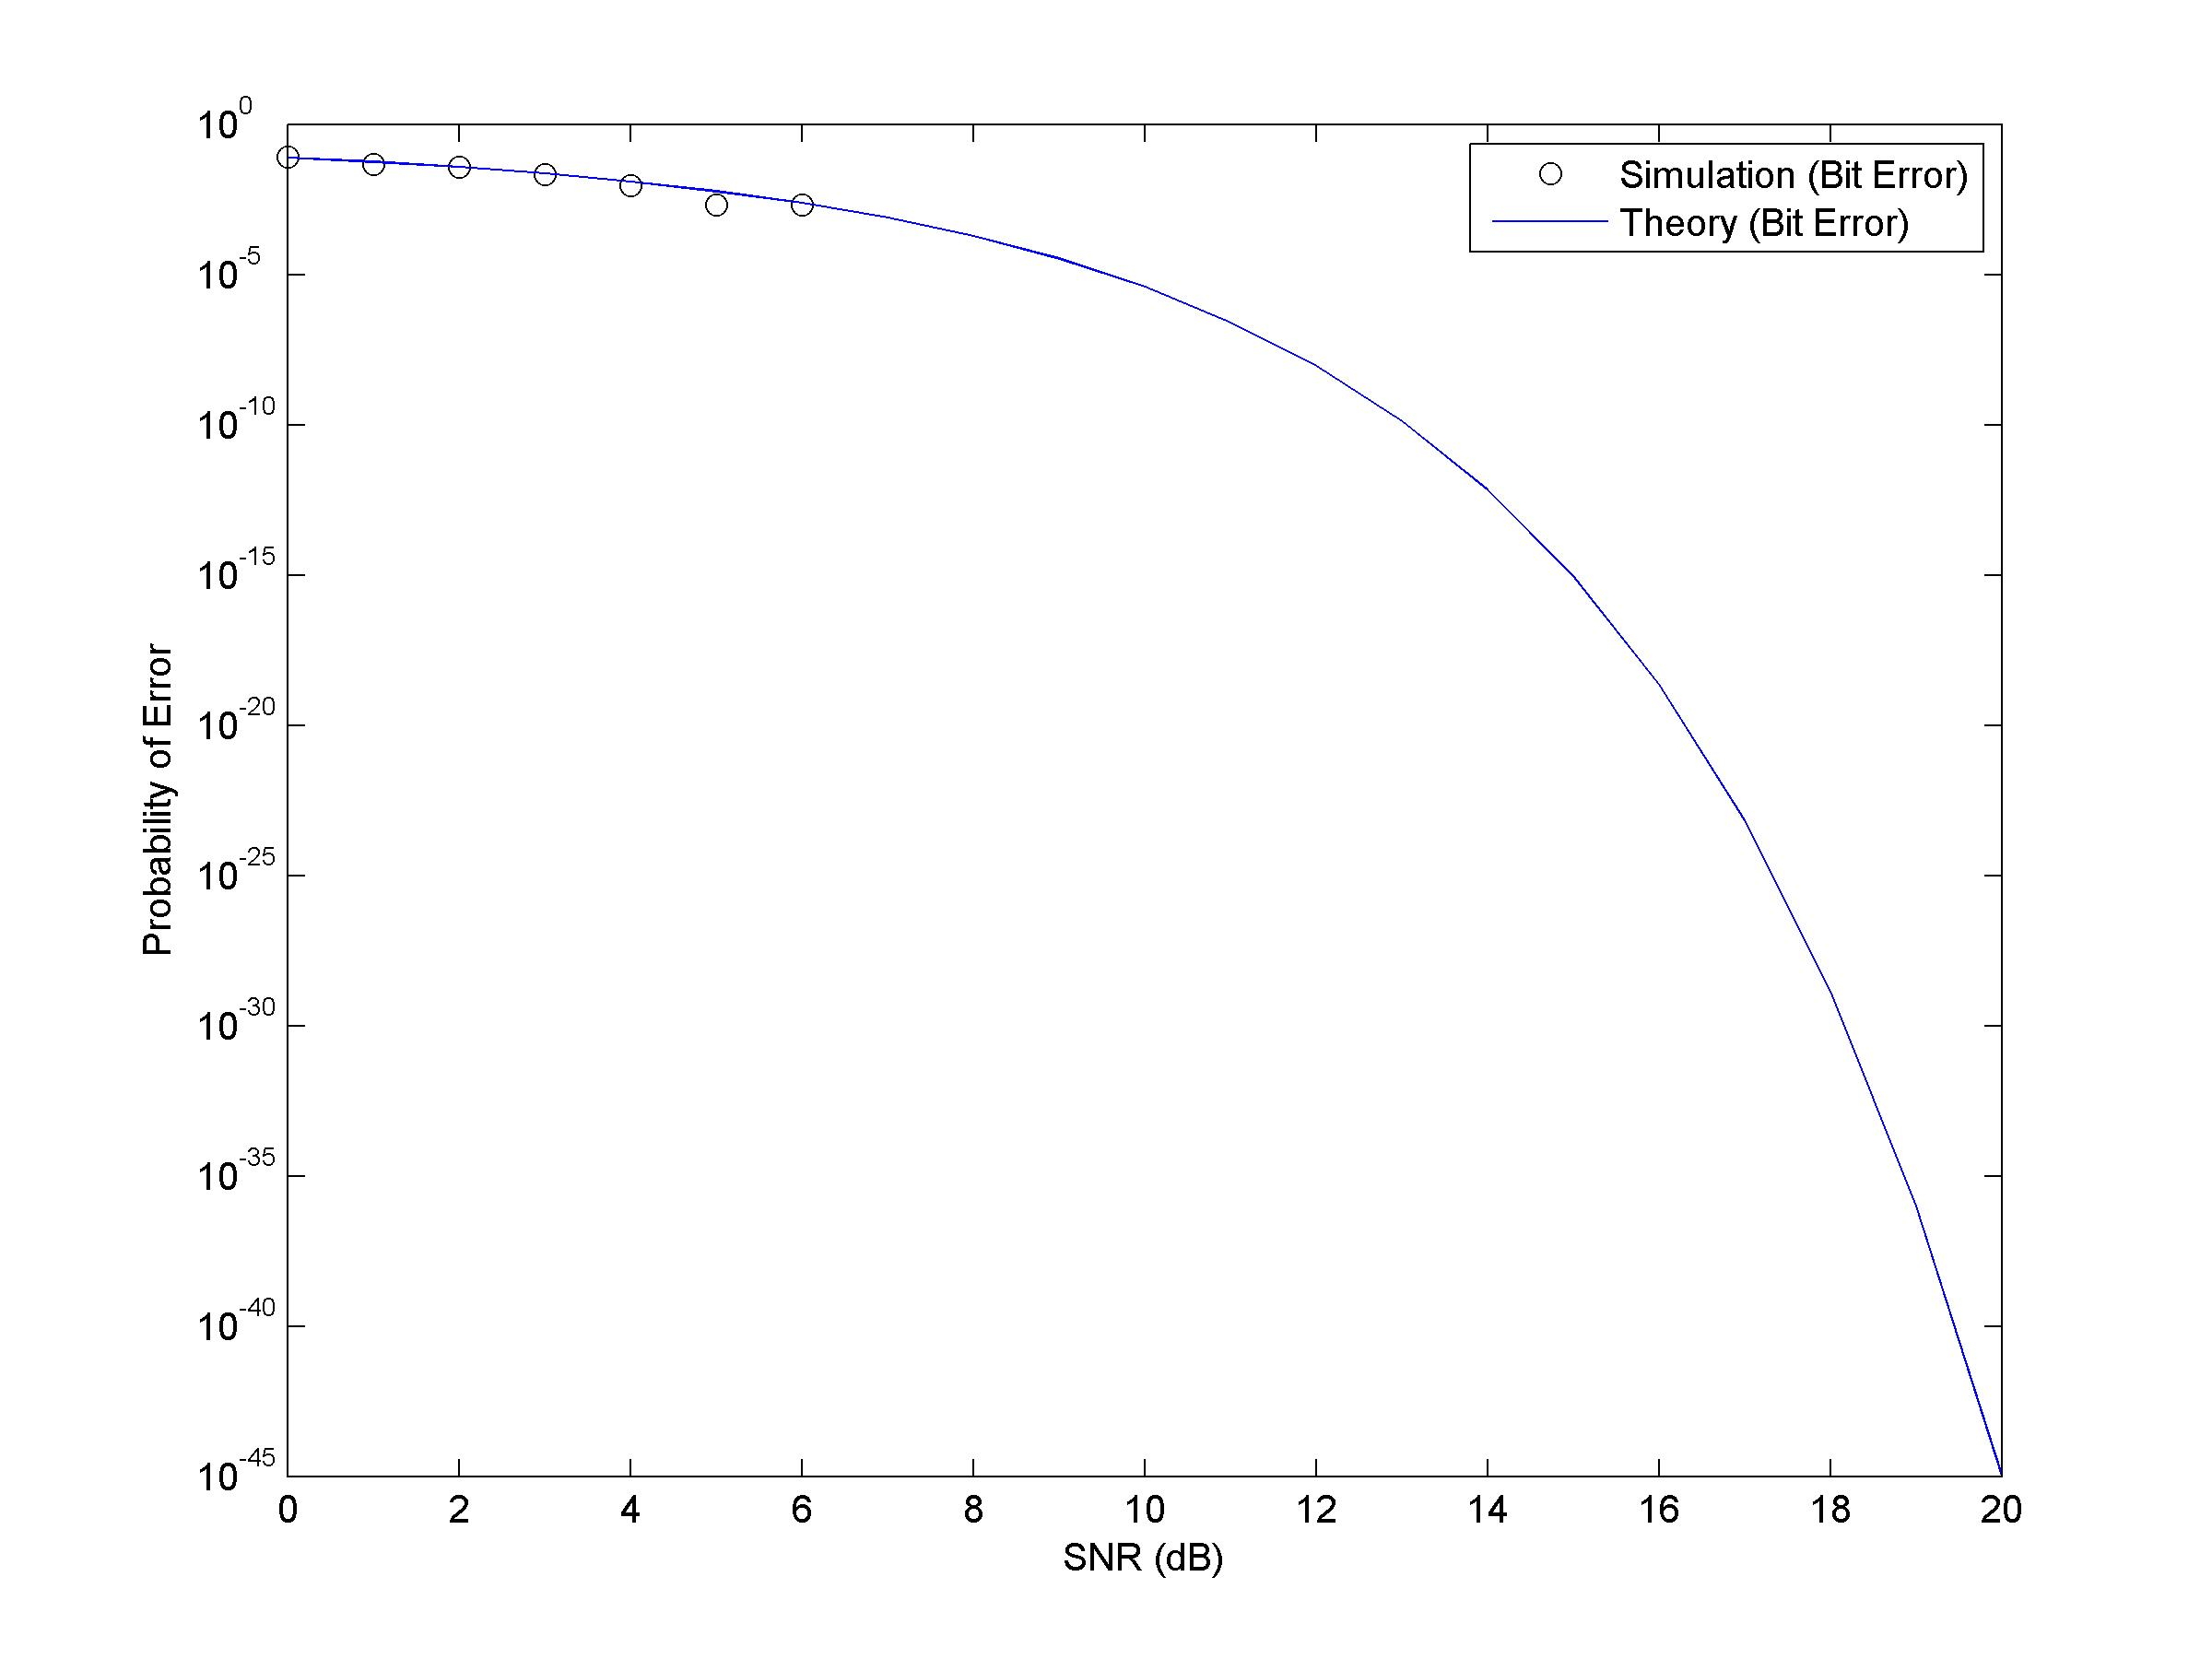
\includegraphics[width=1.3\textwidth]{bpSNRfo3.jpg}
\caption{BPSK Theoretical and Experimental error rates versus different SNR levels at a frequency offset of 1 Hz}
\end{figure}

\begin{figure}[H]
\centering
\hspace*{-2cm}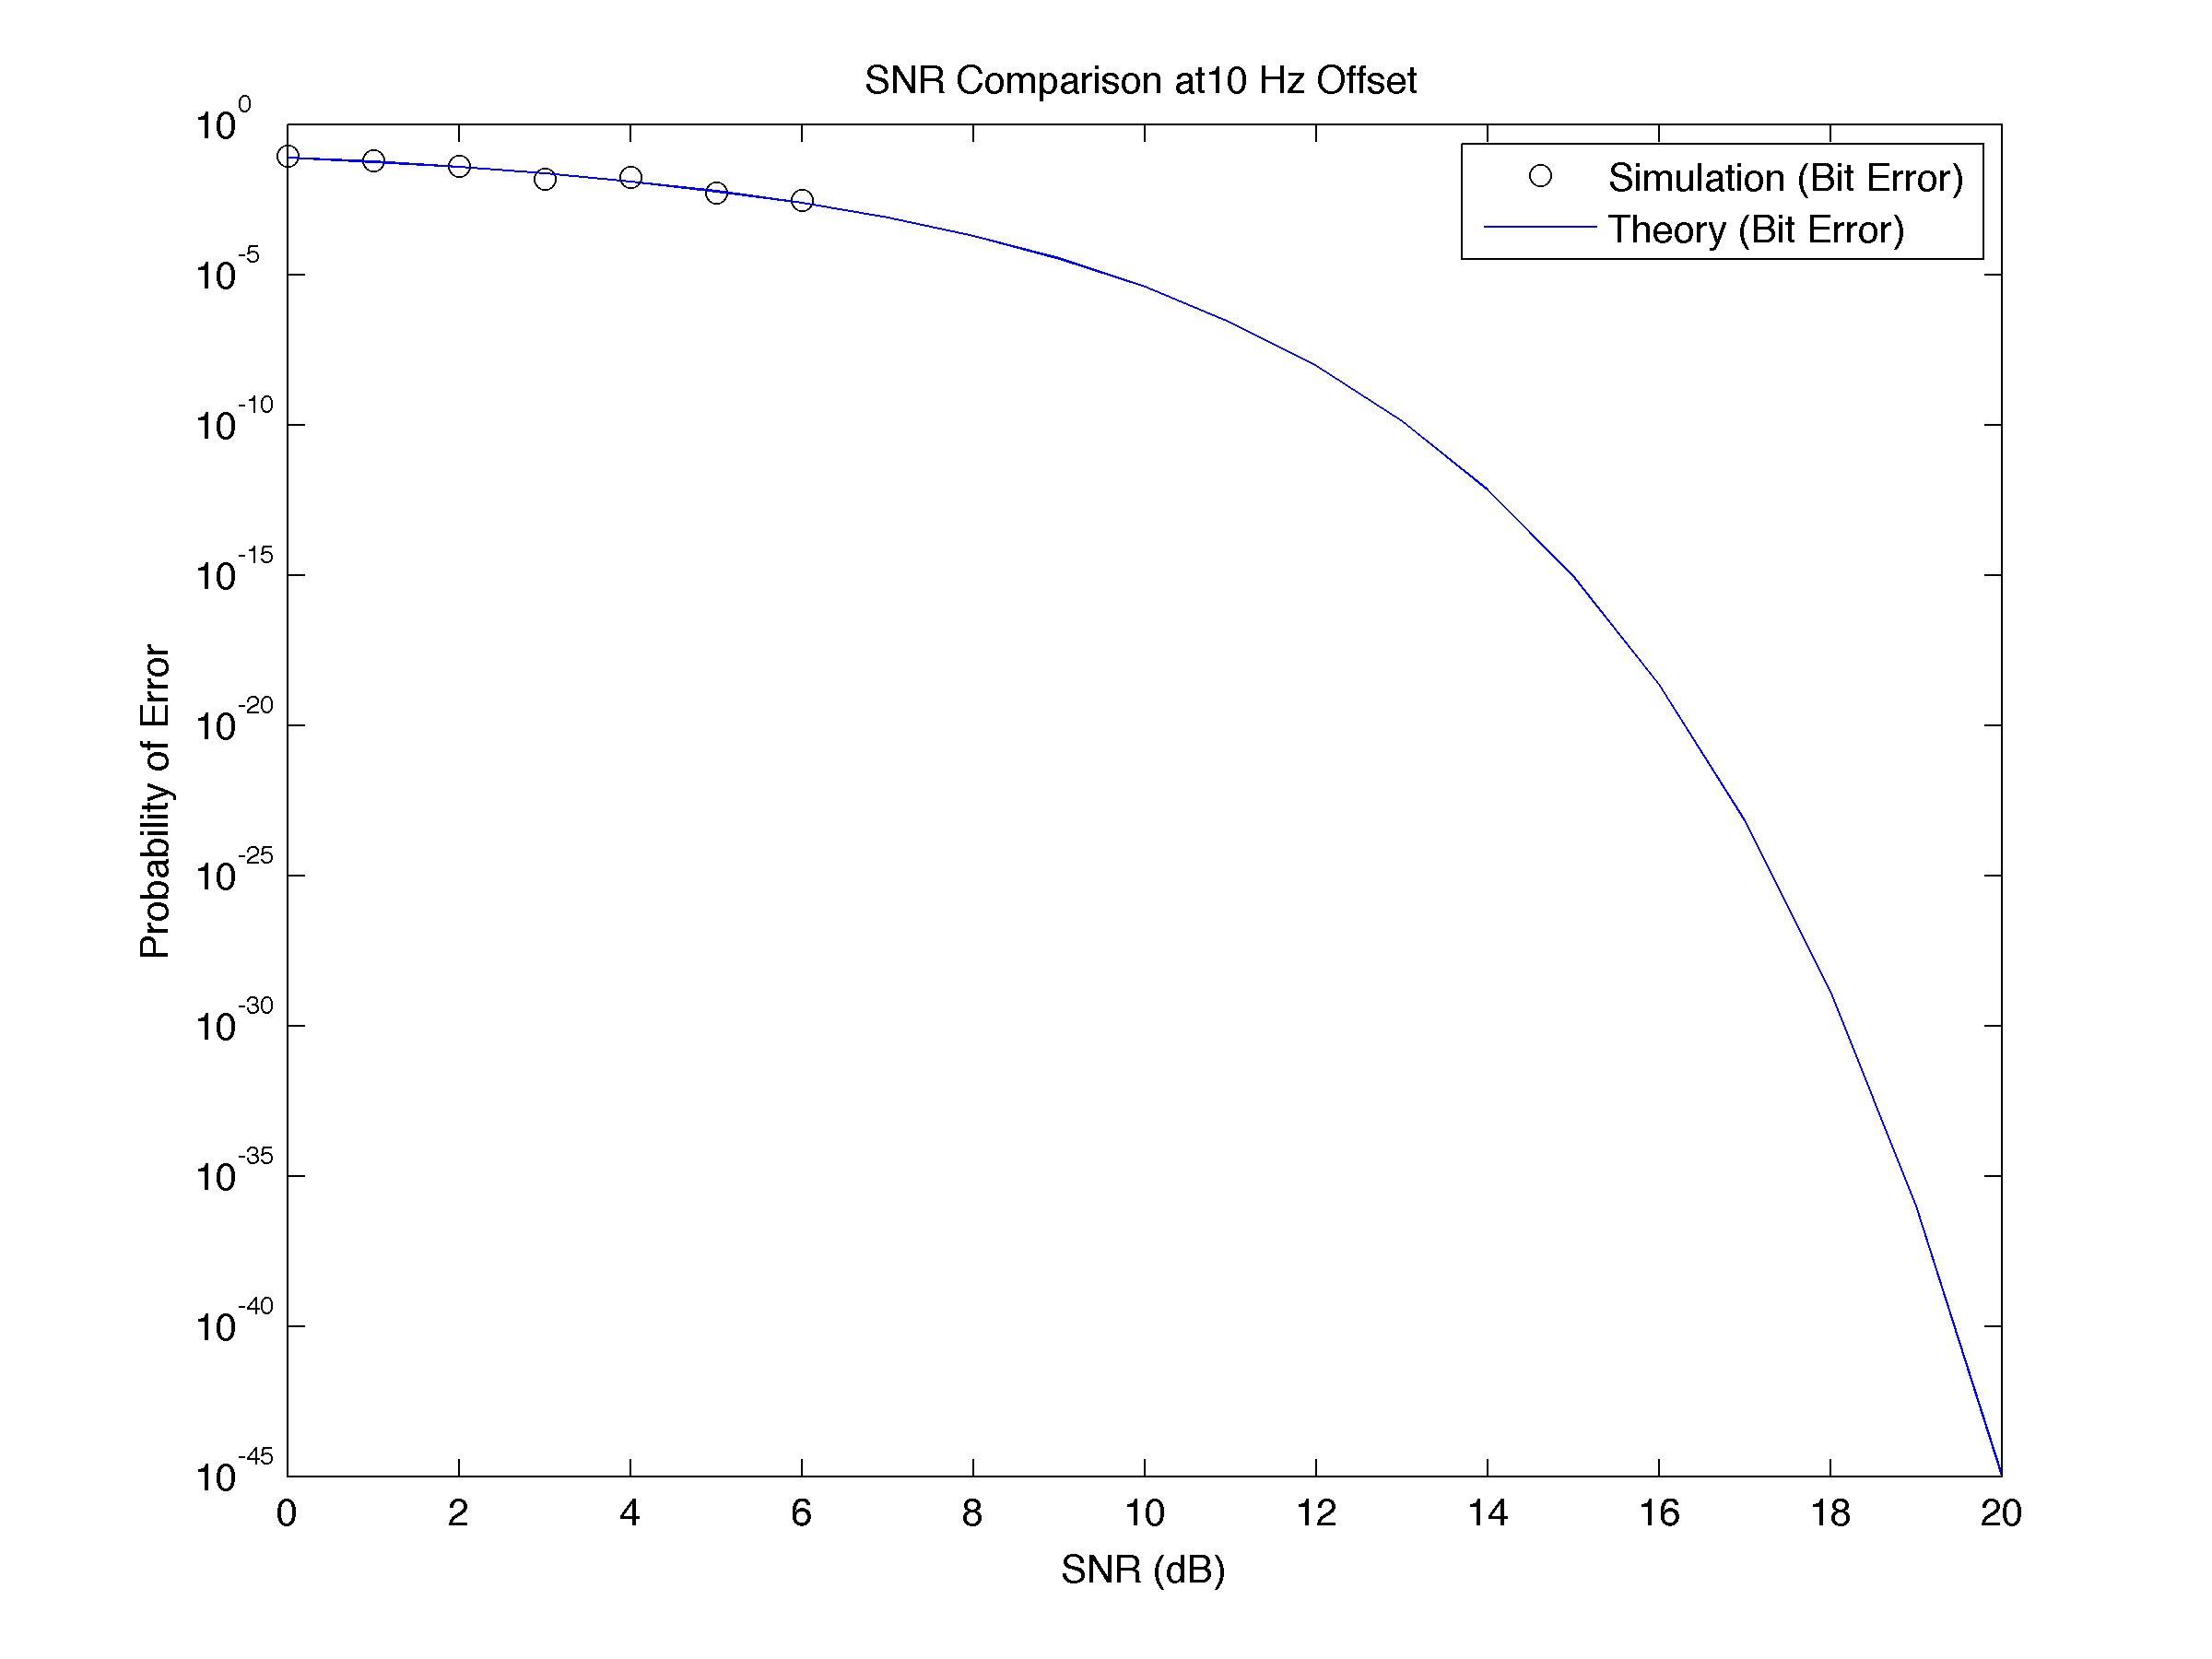
\includegraphics[width=1.3\textwidth]{bpSNRfo4.jpg}
\caption{BPSK Theoretical and Experimental error rates versus different SNR levels at a frequency offset of 10 Hz}
\end{figure}


\subsubsection{QPSK with Frequency Offset}
\begin{figure}[H]
\centering
\hspace*{-2cm}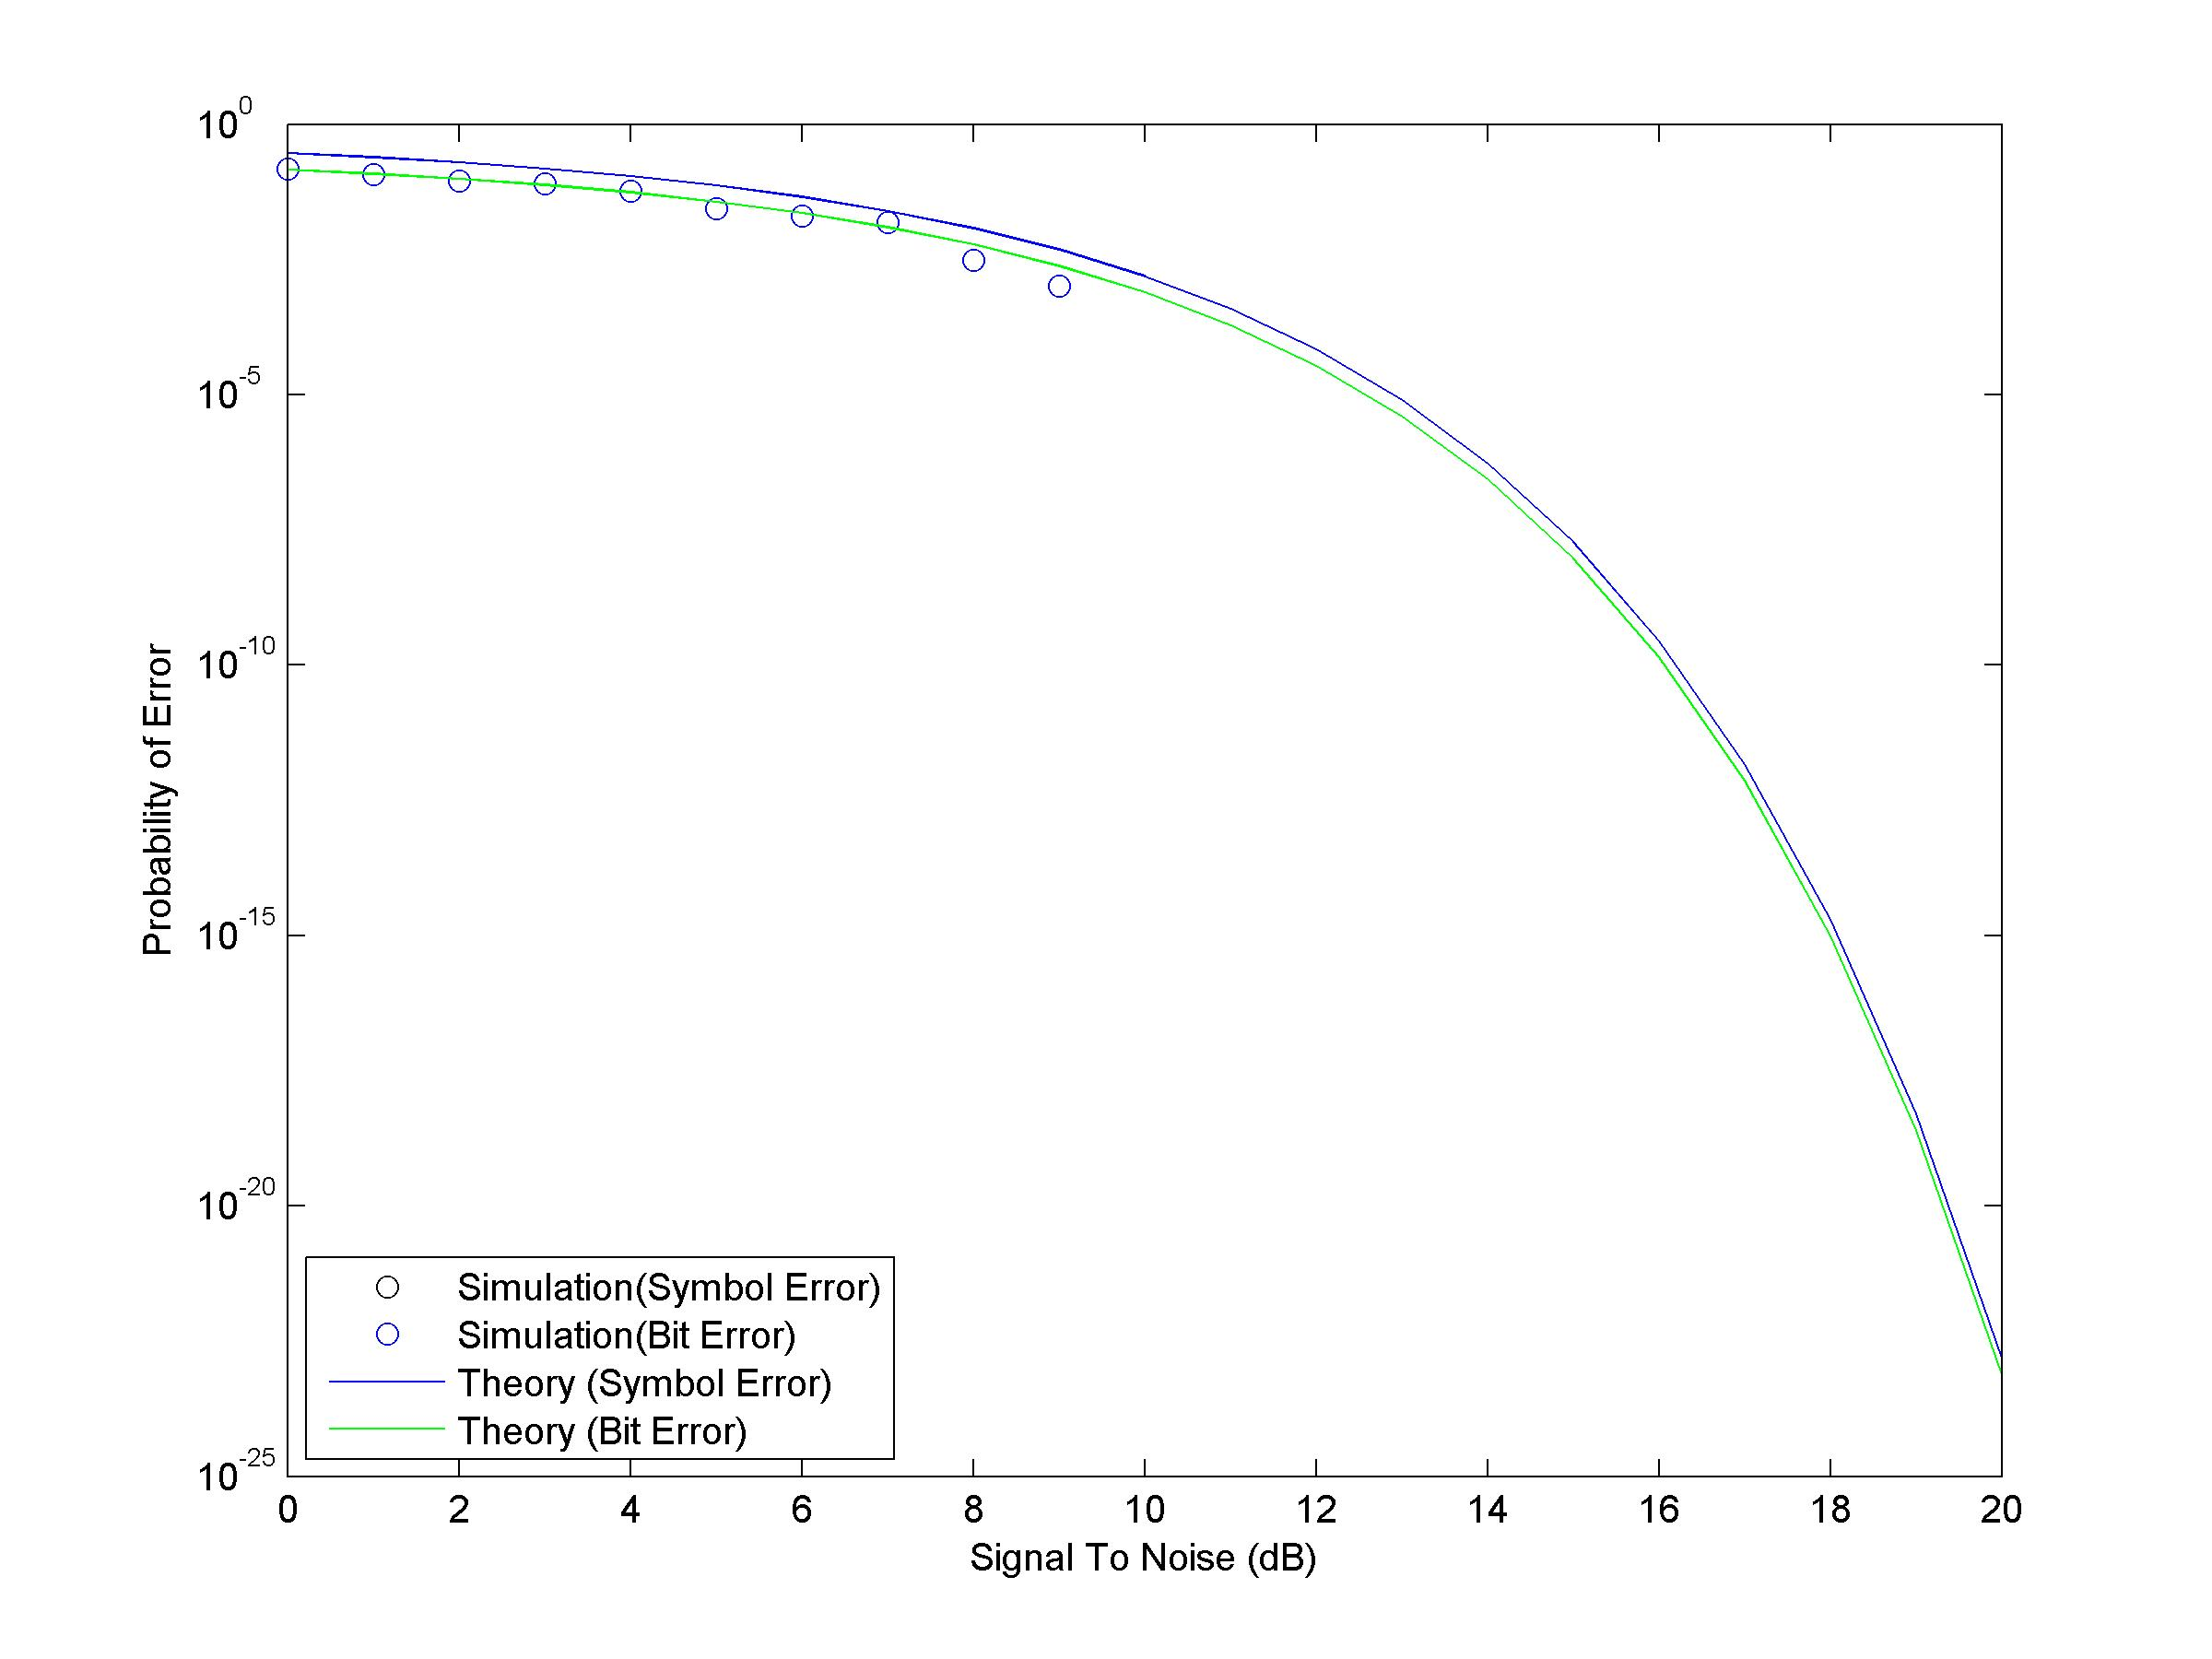
\includegraphics[width=1.3\textwidth]{qpSNRfo1.jpg}
\caption{QPSK Theoretical and Experimental error rates versus different SNR levels at a frequency offset of 0.01 Hz}
\end{figure}

\begin{figure}[H]
\centering
\hspace*{-2cm}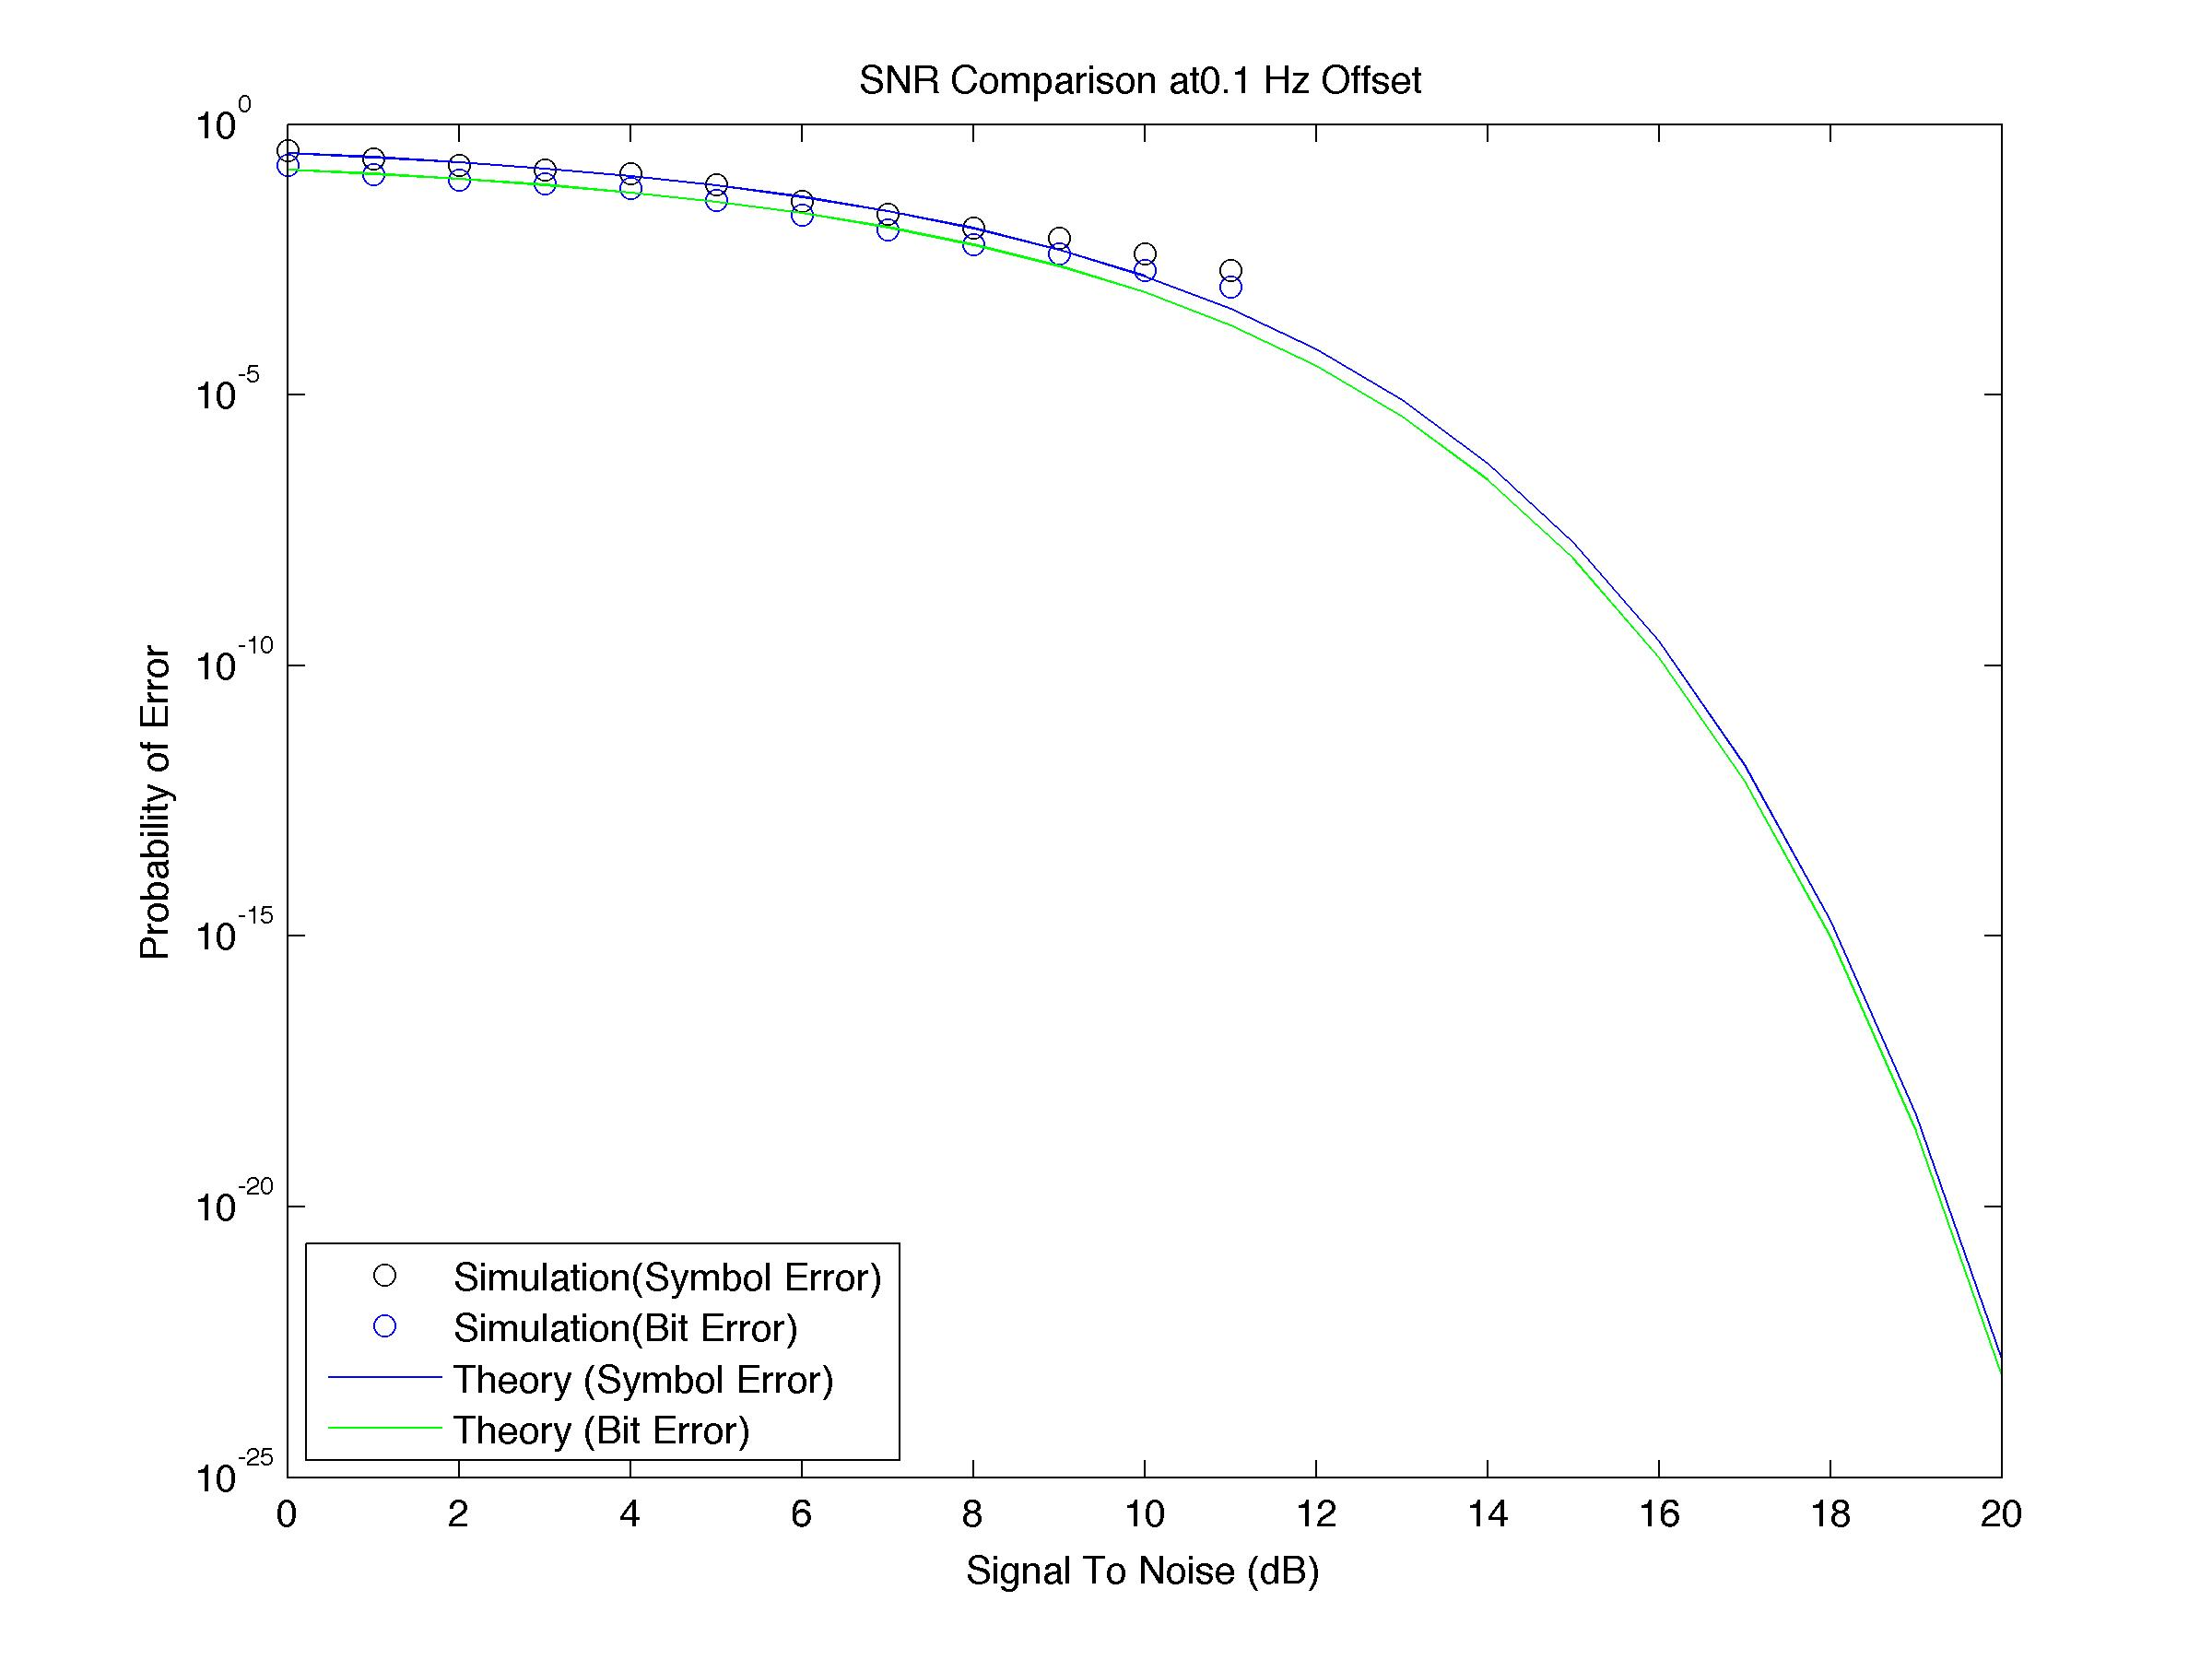
\includegraphics[width=1.3\textwidth]{qpSNRfo2.jpg}
\caption{QPSK Theoretical and Experimental error rates versus different SNR levels at a frequency offset of 0.1 Hz}
\end{figure}

\begin{figure}[H]
\centering
\hspace*{-2cm}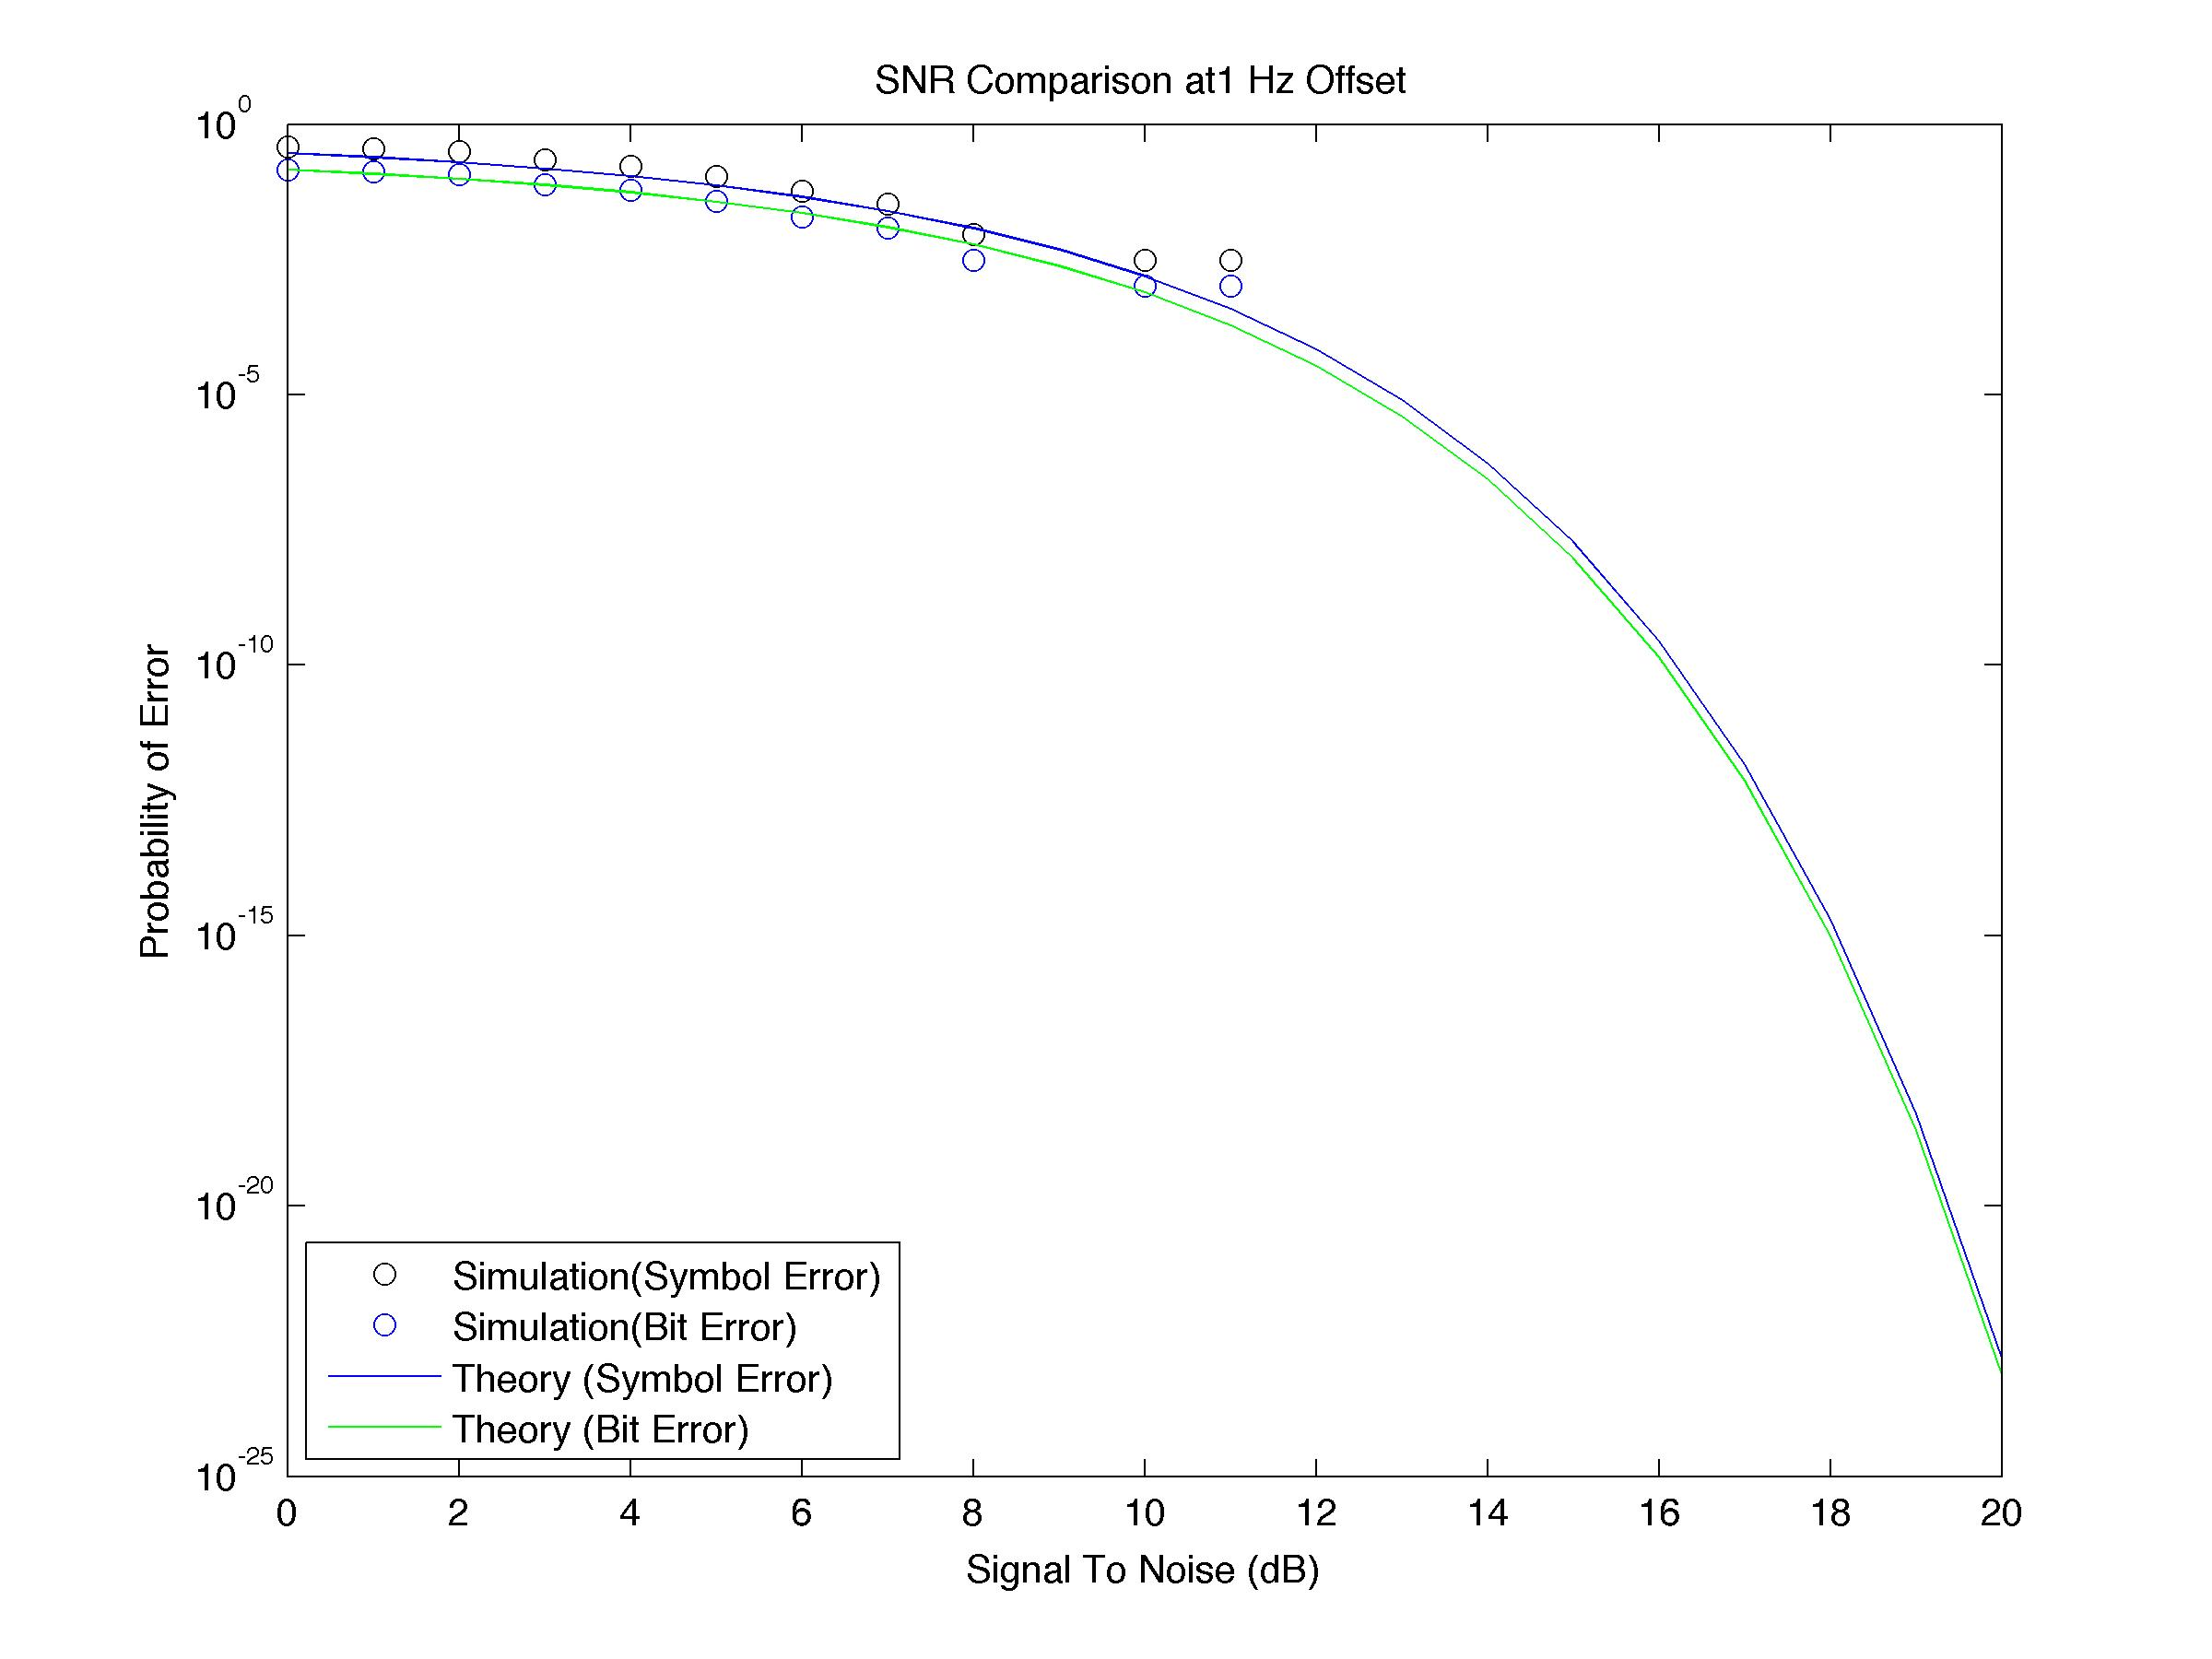
\includegraphics[width=1.3\textwidth]{qpSNRfo3.jpg}
\caption{QPSK Theoretical and Experimental error rates versus different SNR levels at a frequency offset of 1 Hz}
\end{figure}

\begin{figure}[H]
\centering
\hspace*{-2cm}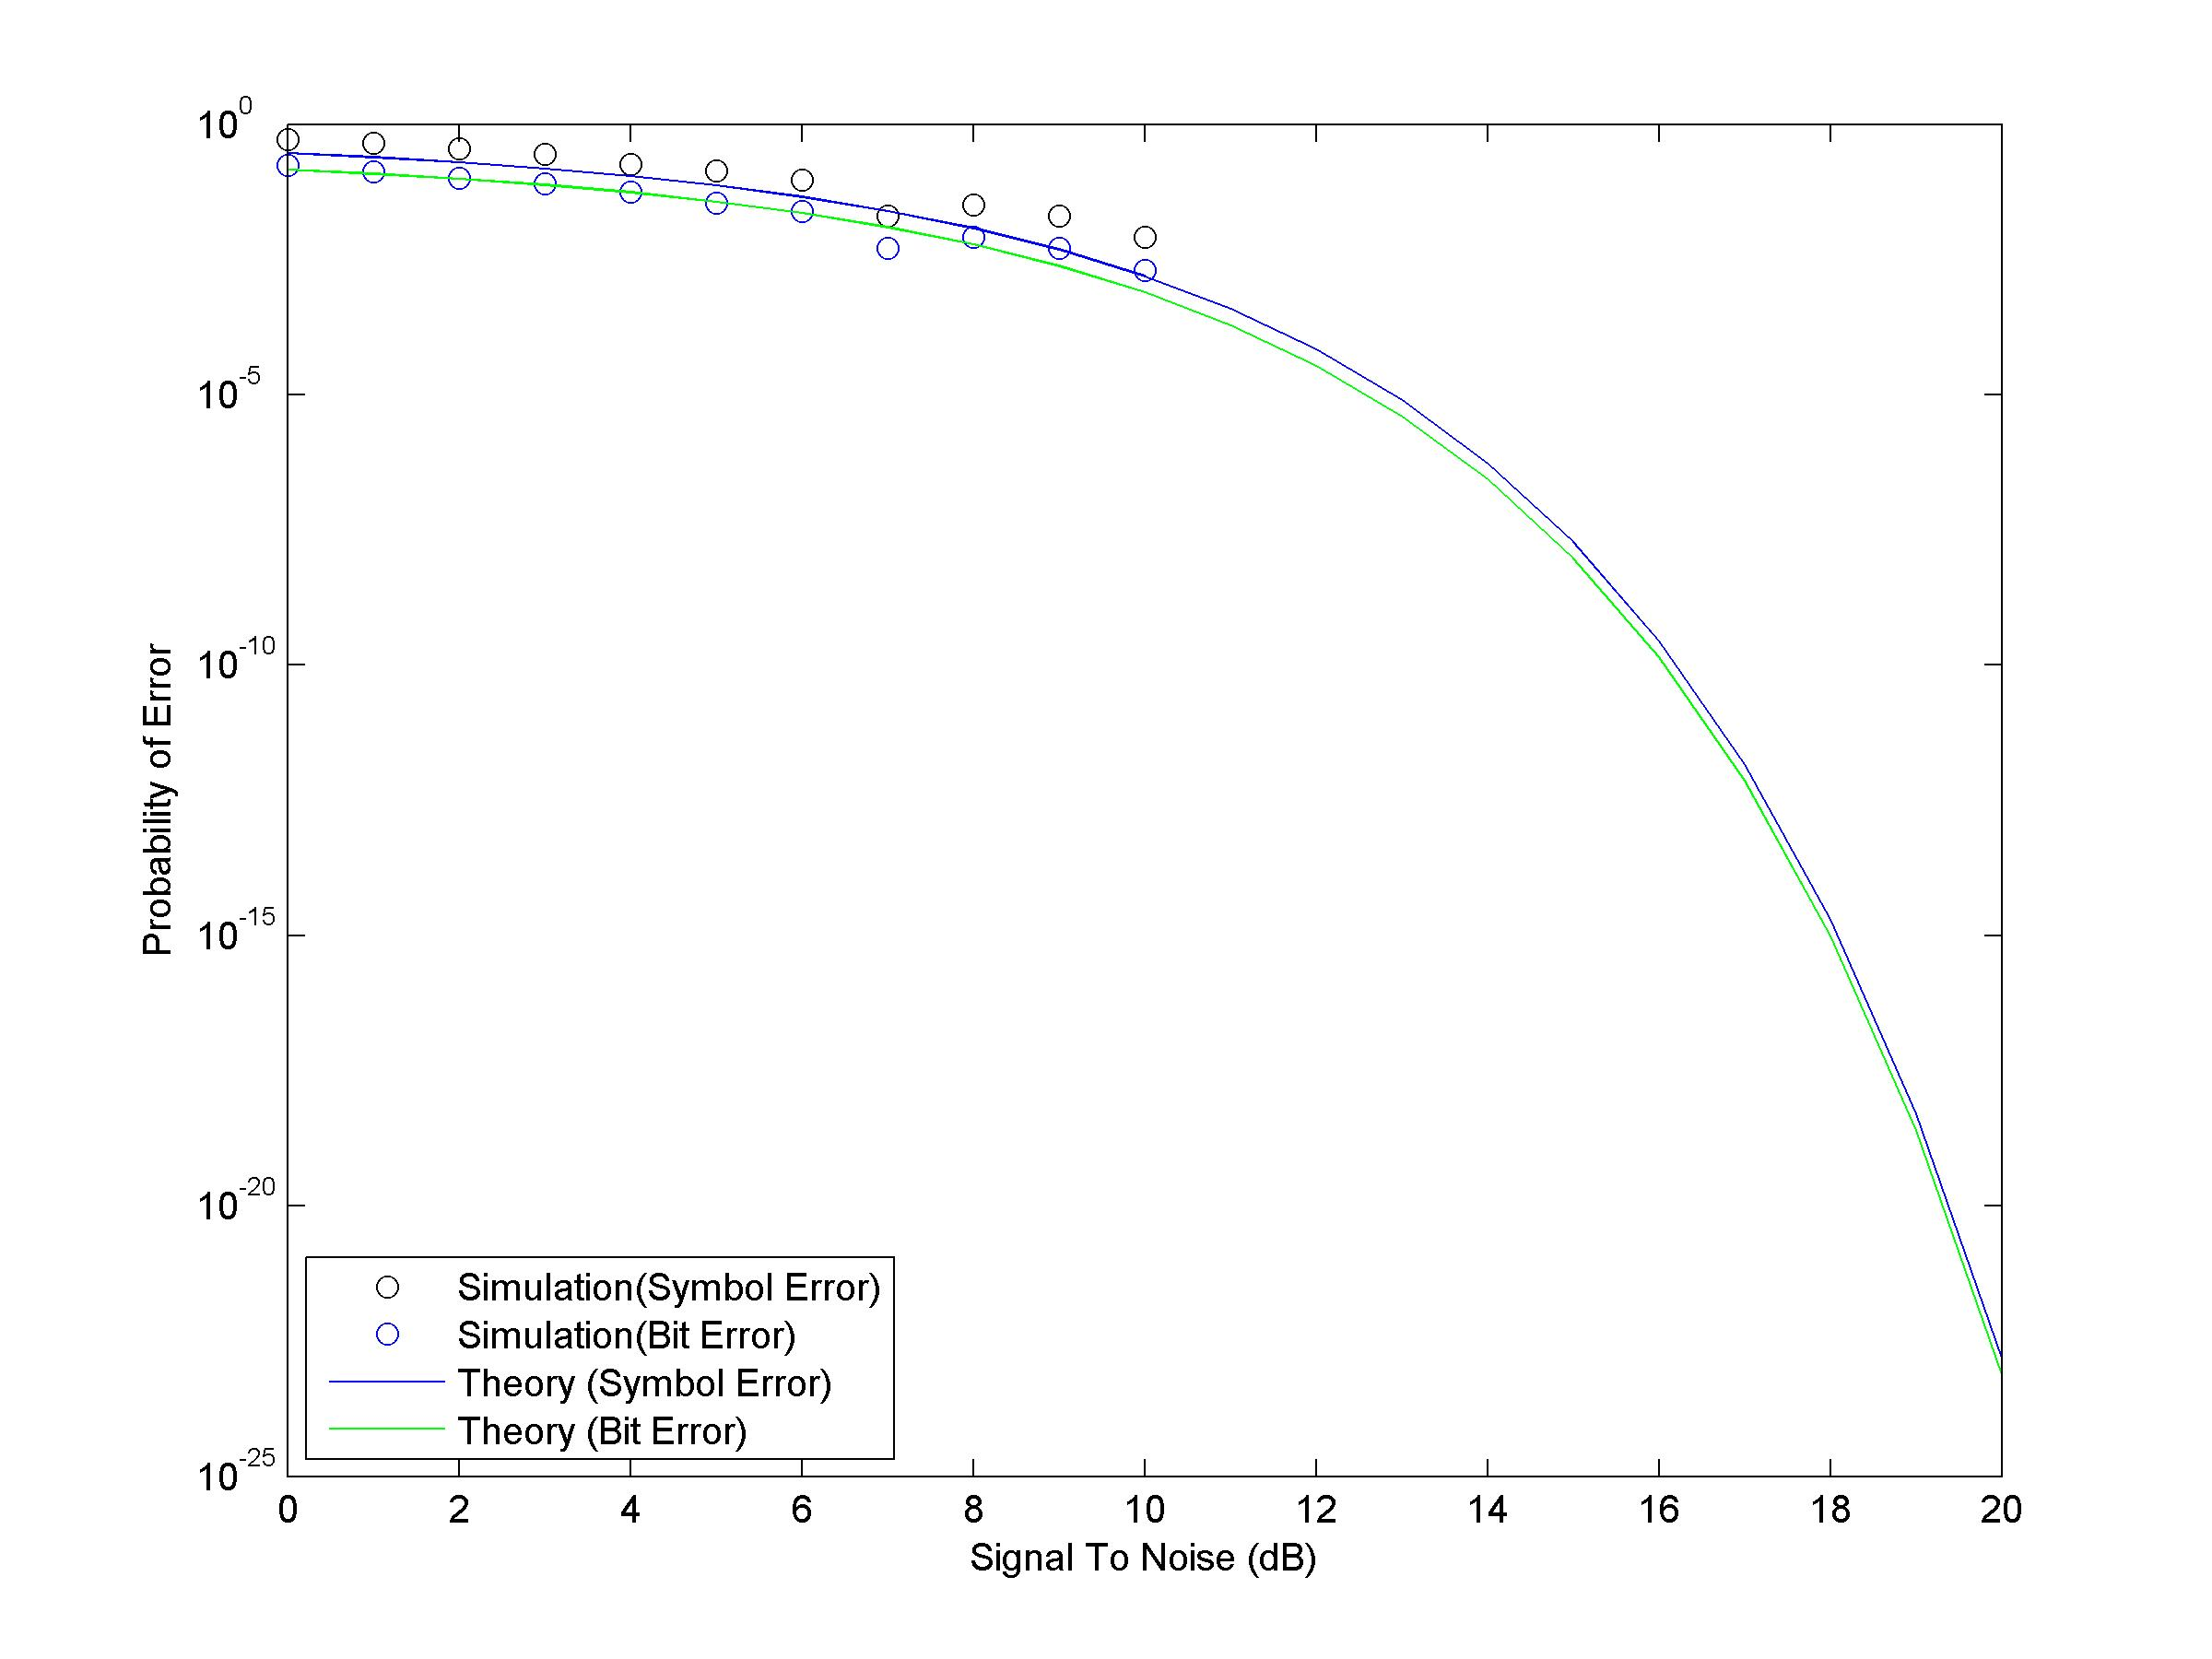
\includegraphics[width=1.3\textwidth]{qpSNRfo4.jpg}
\caption{QPSK Theoretical and Experimental error rates versus different SNR levels at a frequency offset of 10 Hz}
\end{figure}


\subsubsection{16-QAM with Frequency Offset}
\begin{figure}[H]
\centering
\hspace*{-2cm}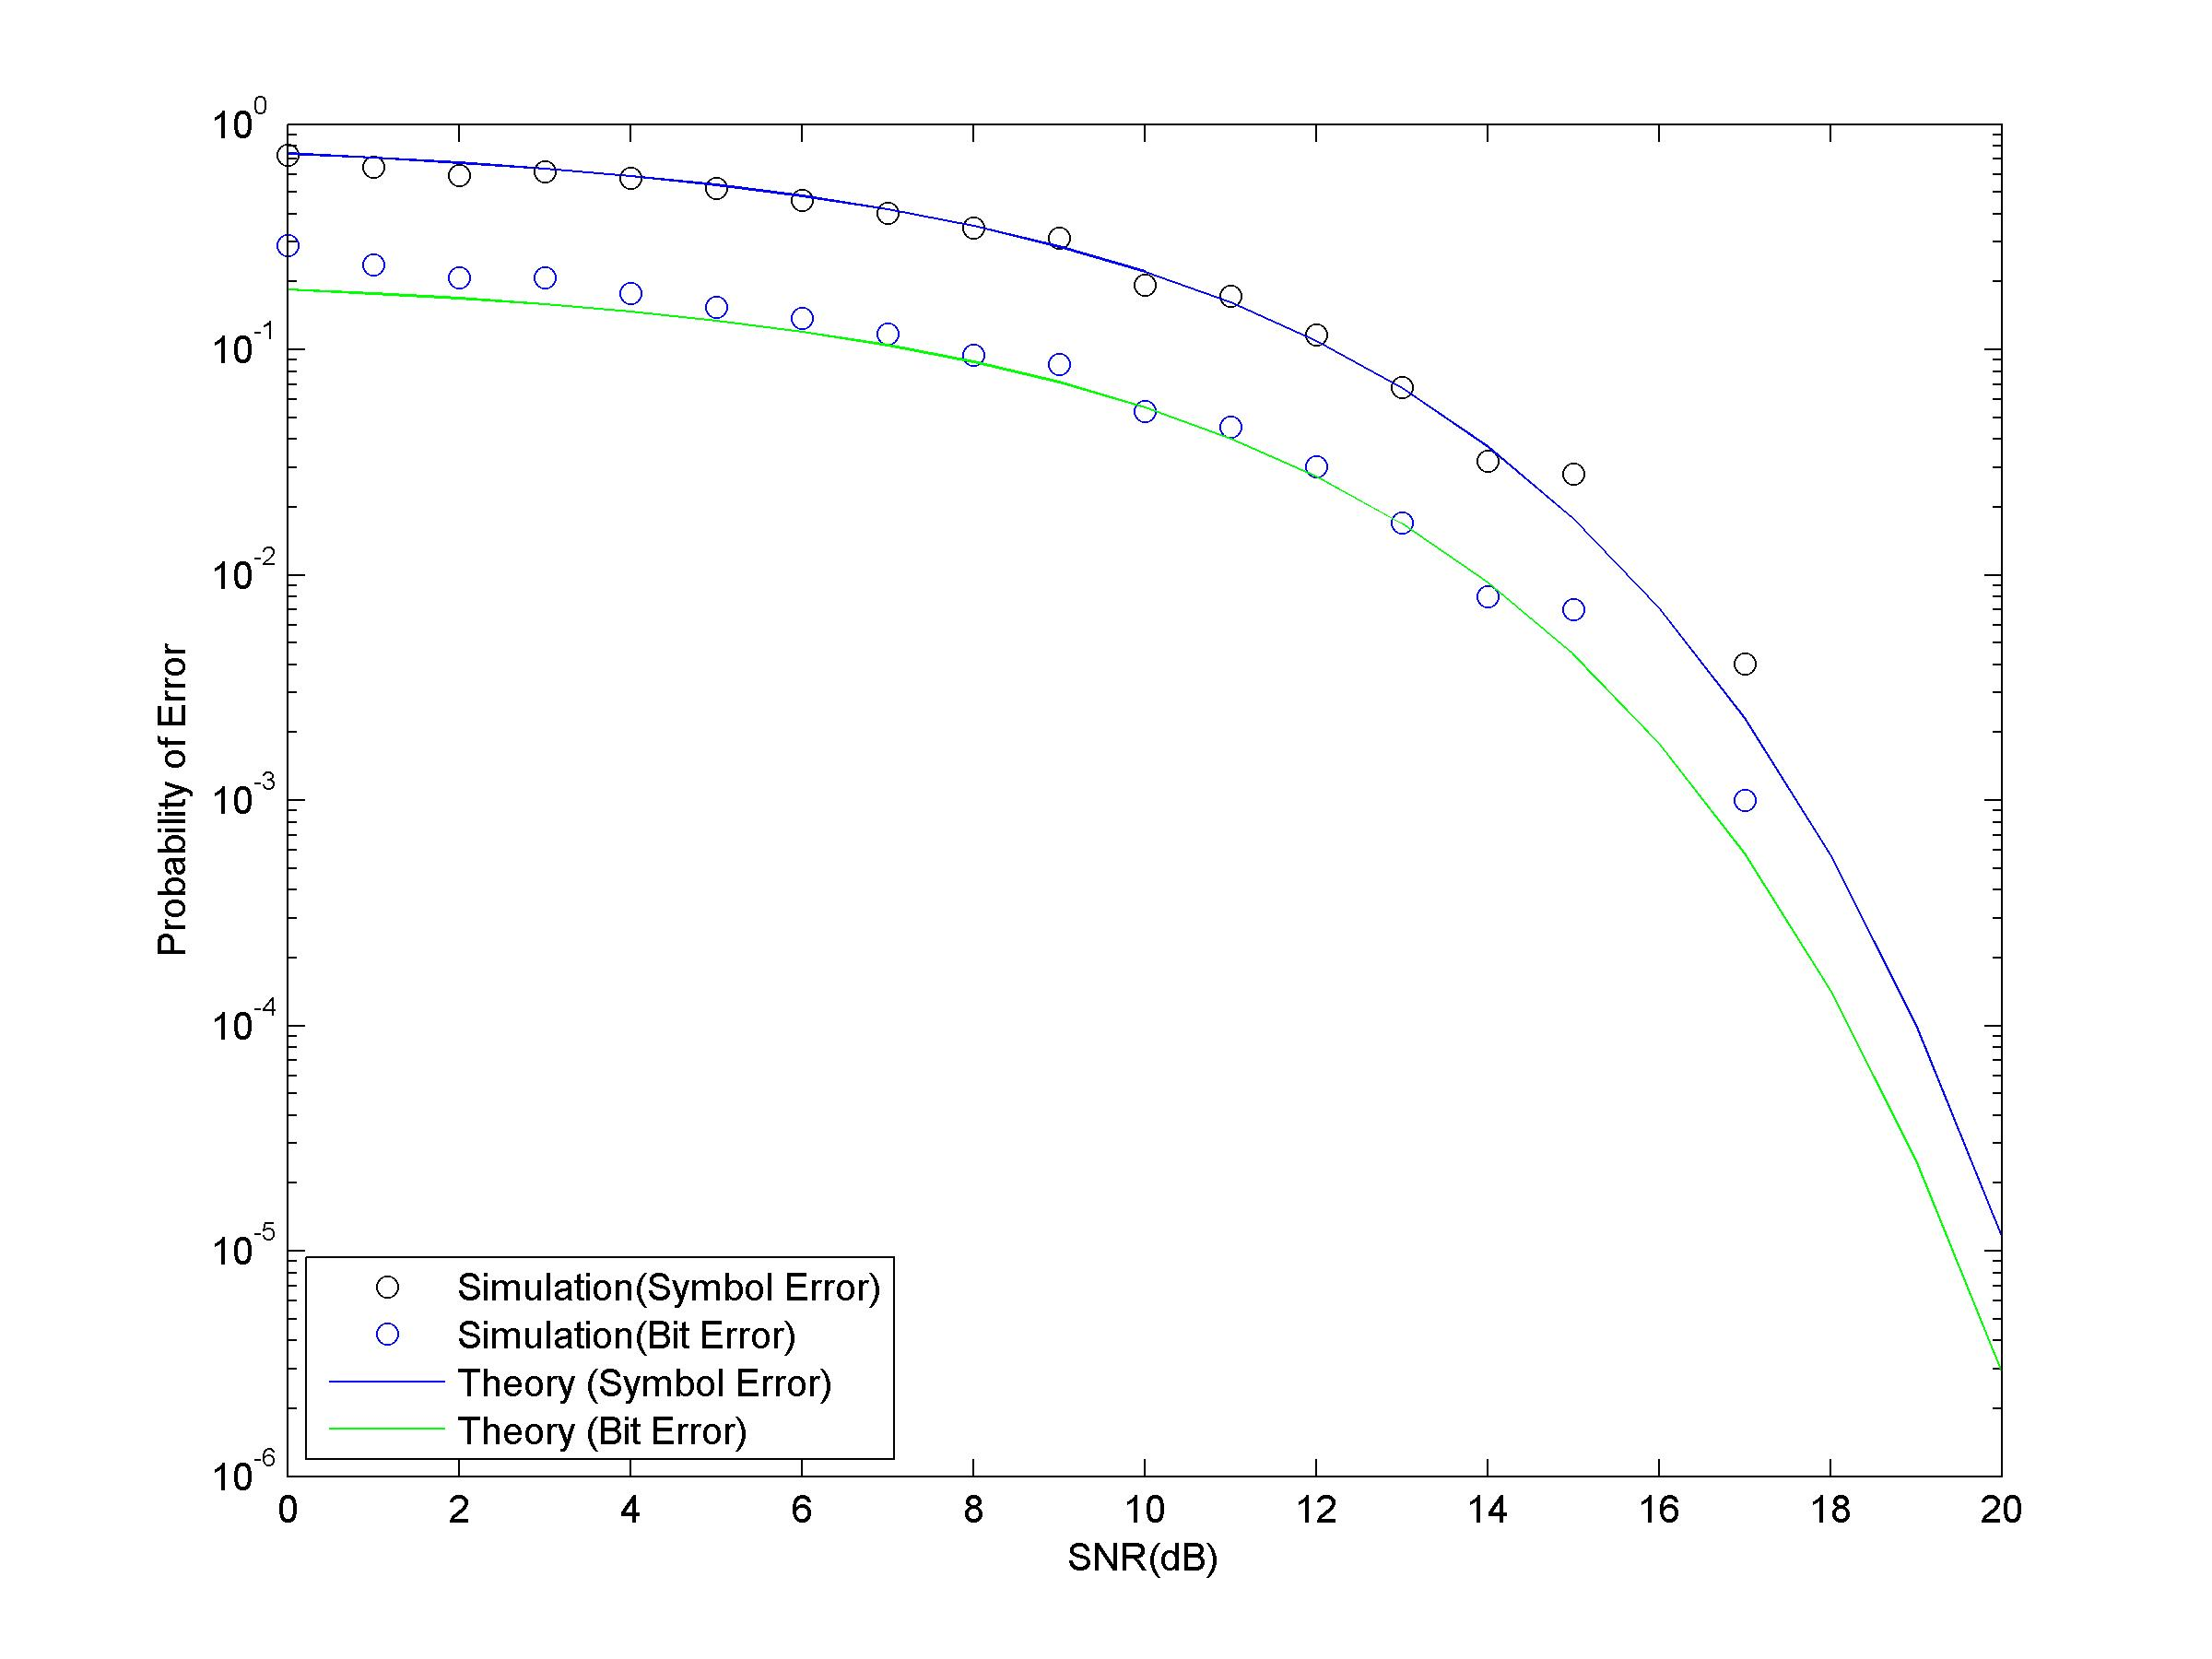
\includegraphics[width=1.3\textwidth]{qam16SNRfo1.jpg}
\caption{16-QAM Theoretical and Experimental error rates versus different SNR levels at a frequency offset of 0.01 Hz}
\end{figure}

\begin{figure}[H]
\centering
\hspace*{-2cm}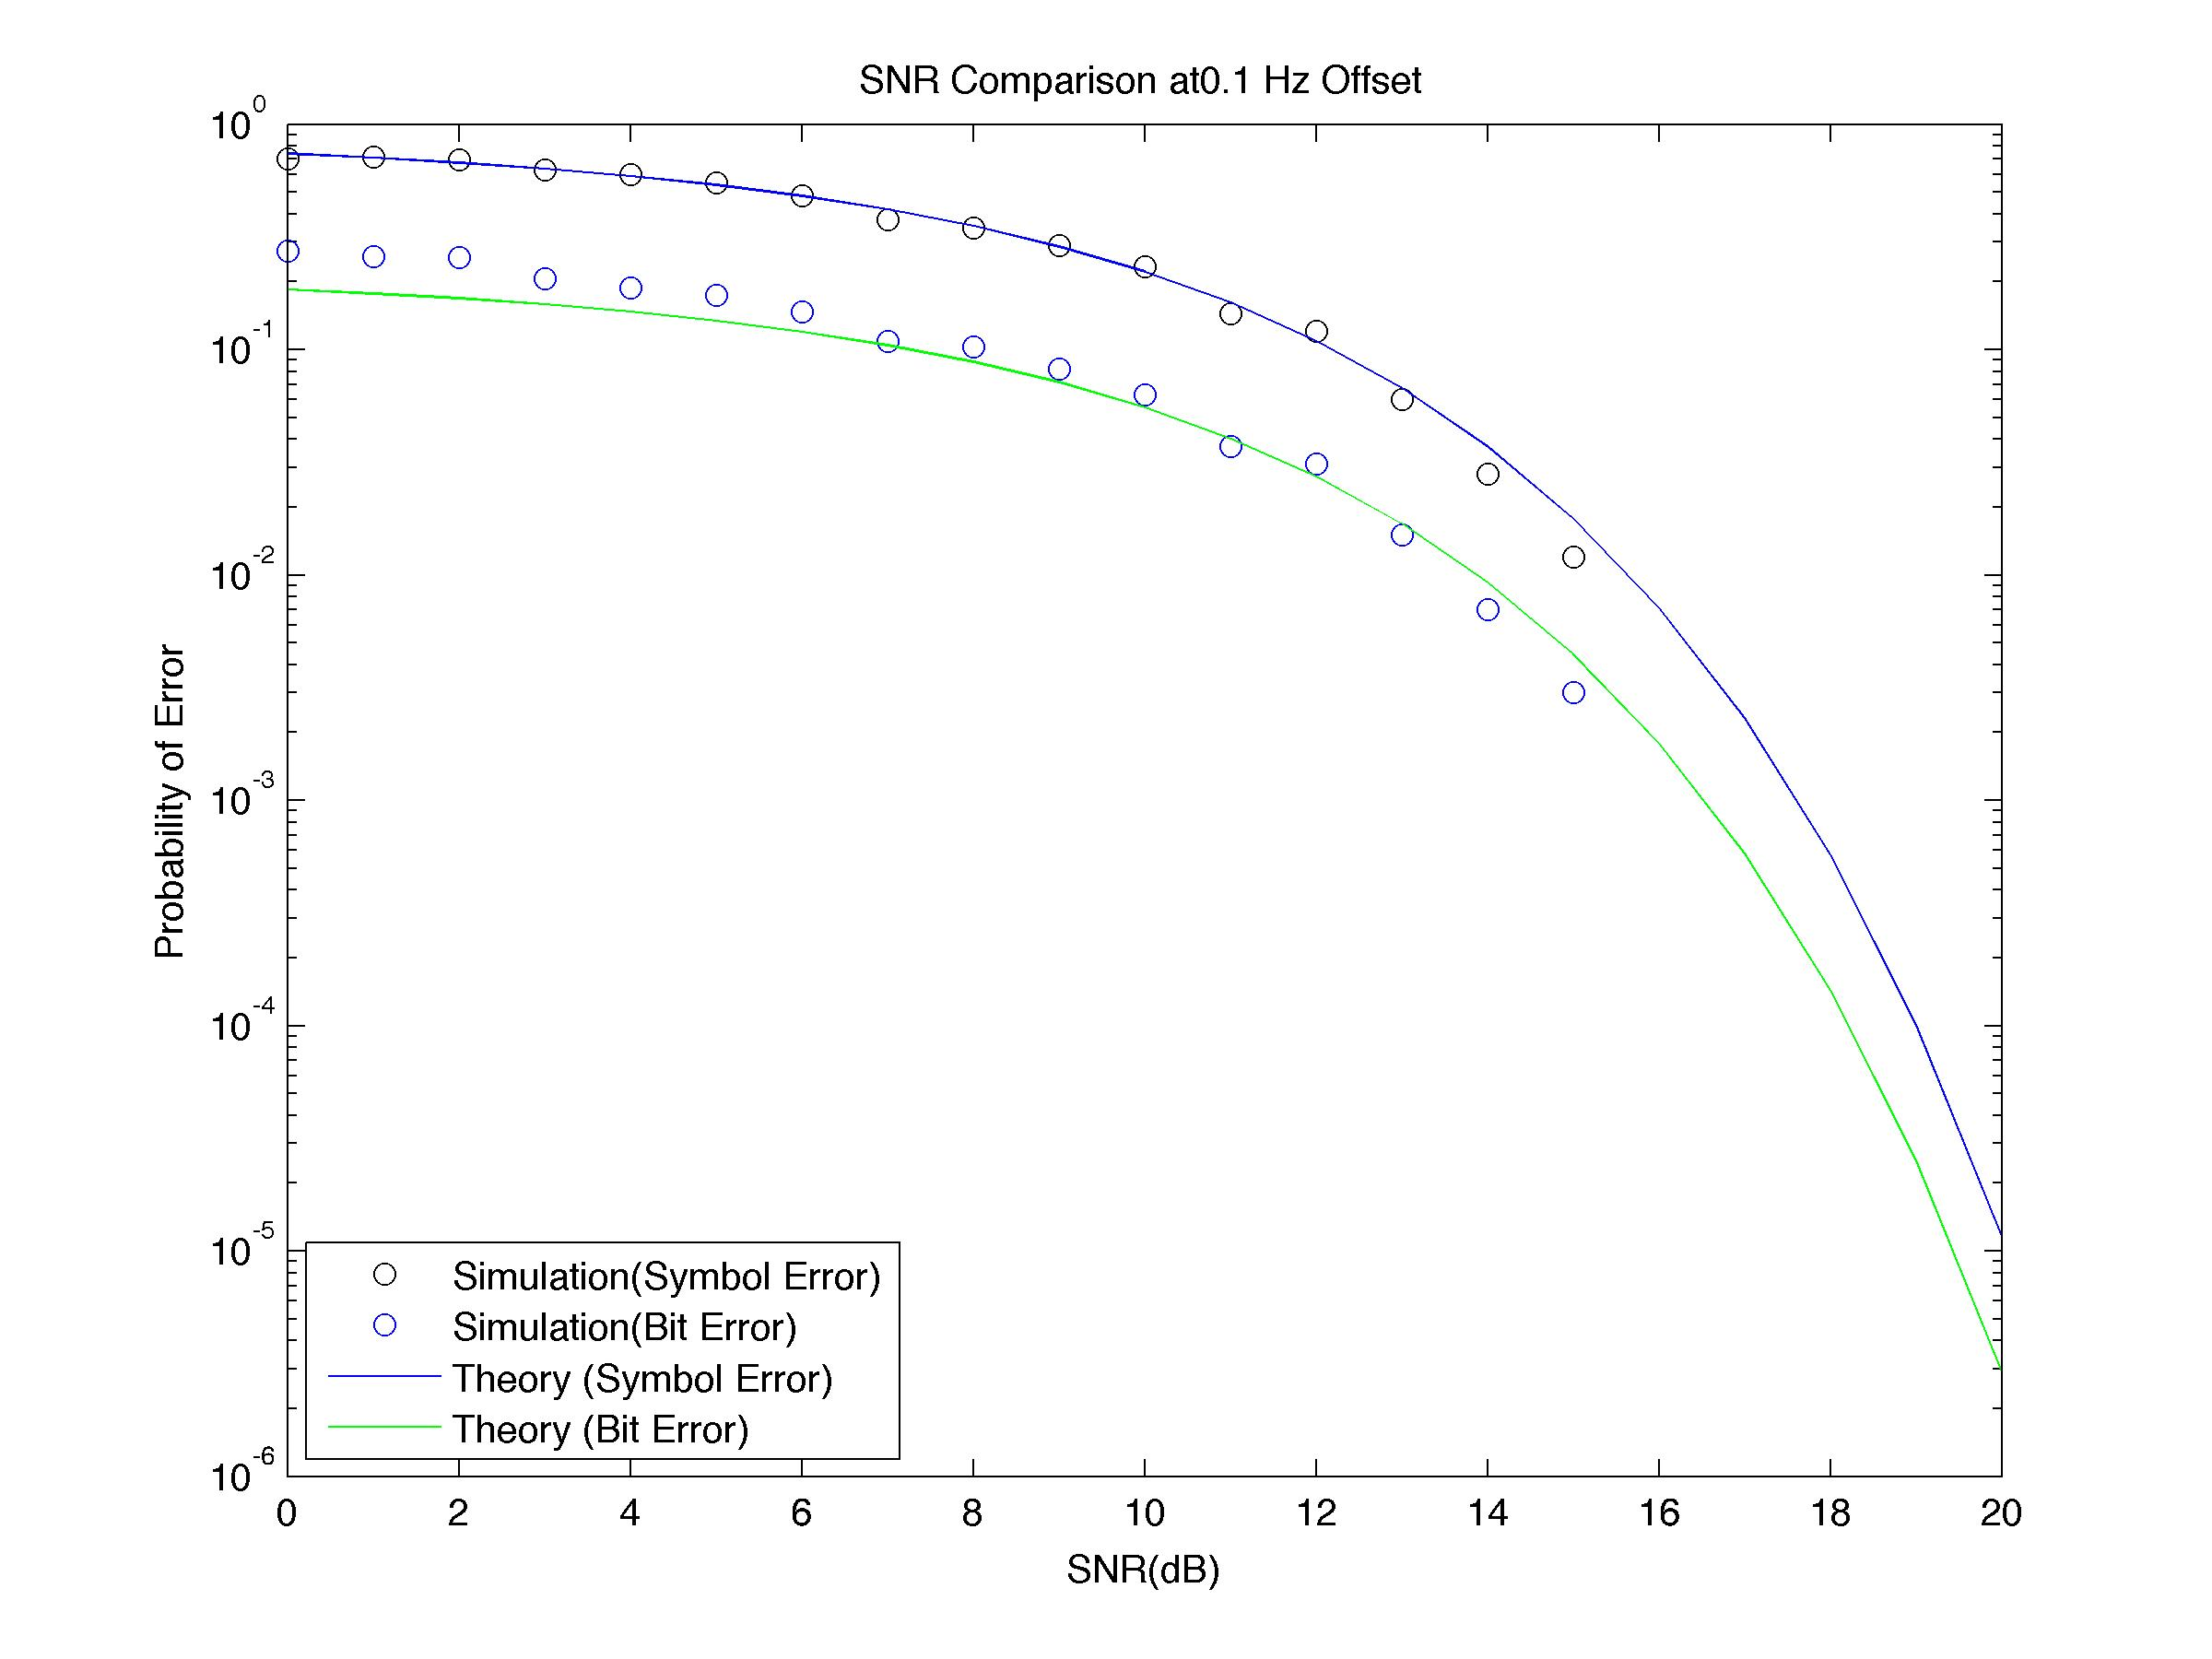
\includegraphics[width=1.3\textwidth]{qam16SNRfo2.jpg}
\caption{16-QAM Theoretical and Experimental error rates versus different SNR levels at a frequency offset of 0.1 Hz}
\end{figure}

\begin{figure}[H]
\centering
\hspace*{-2cm}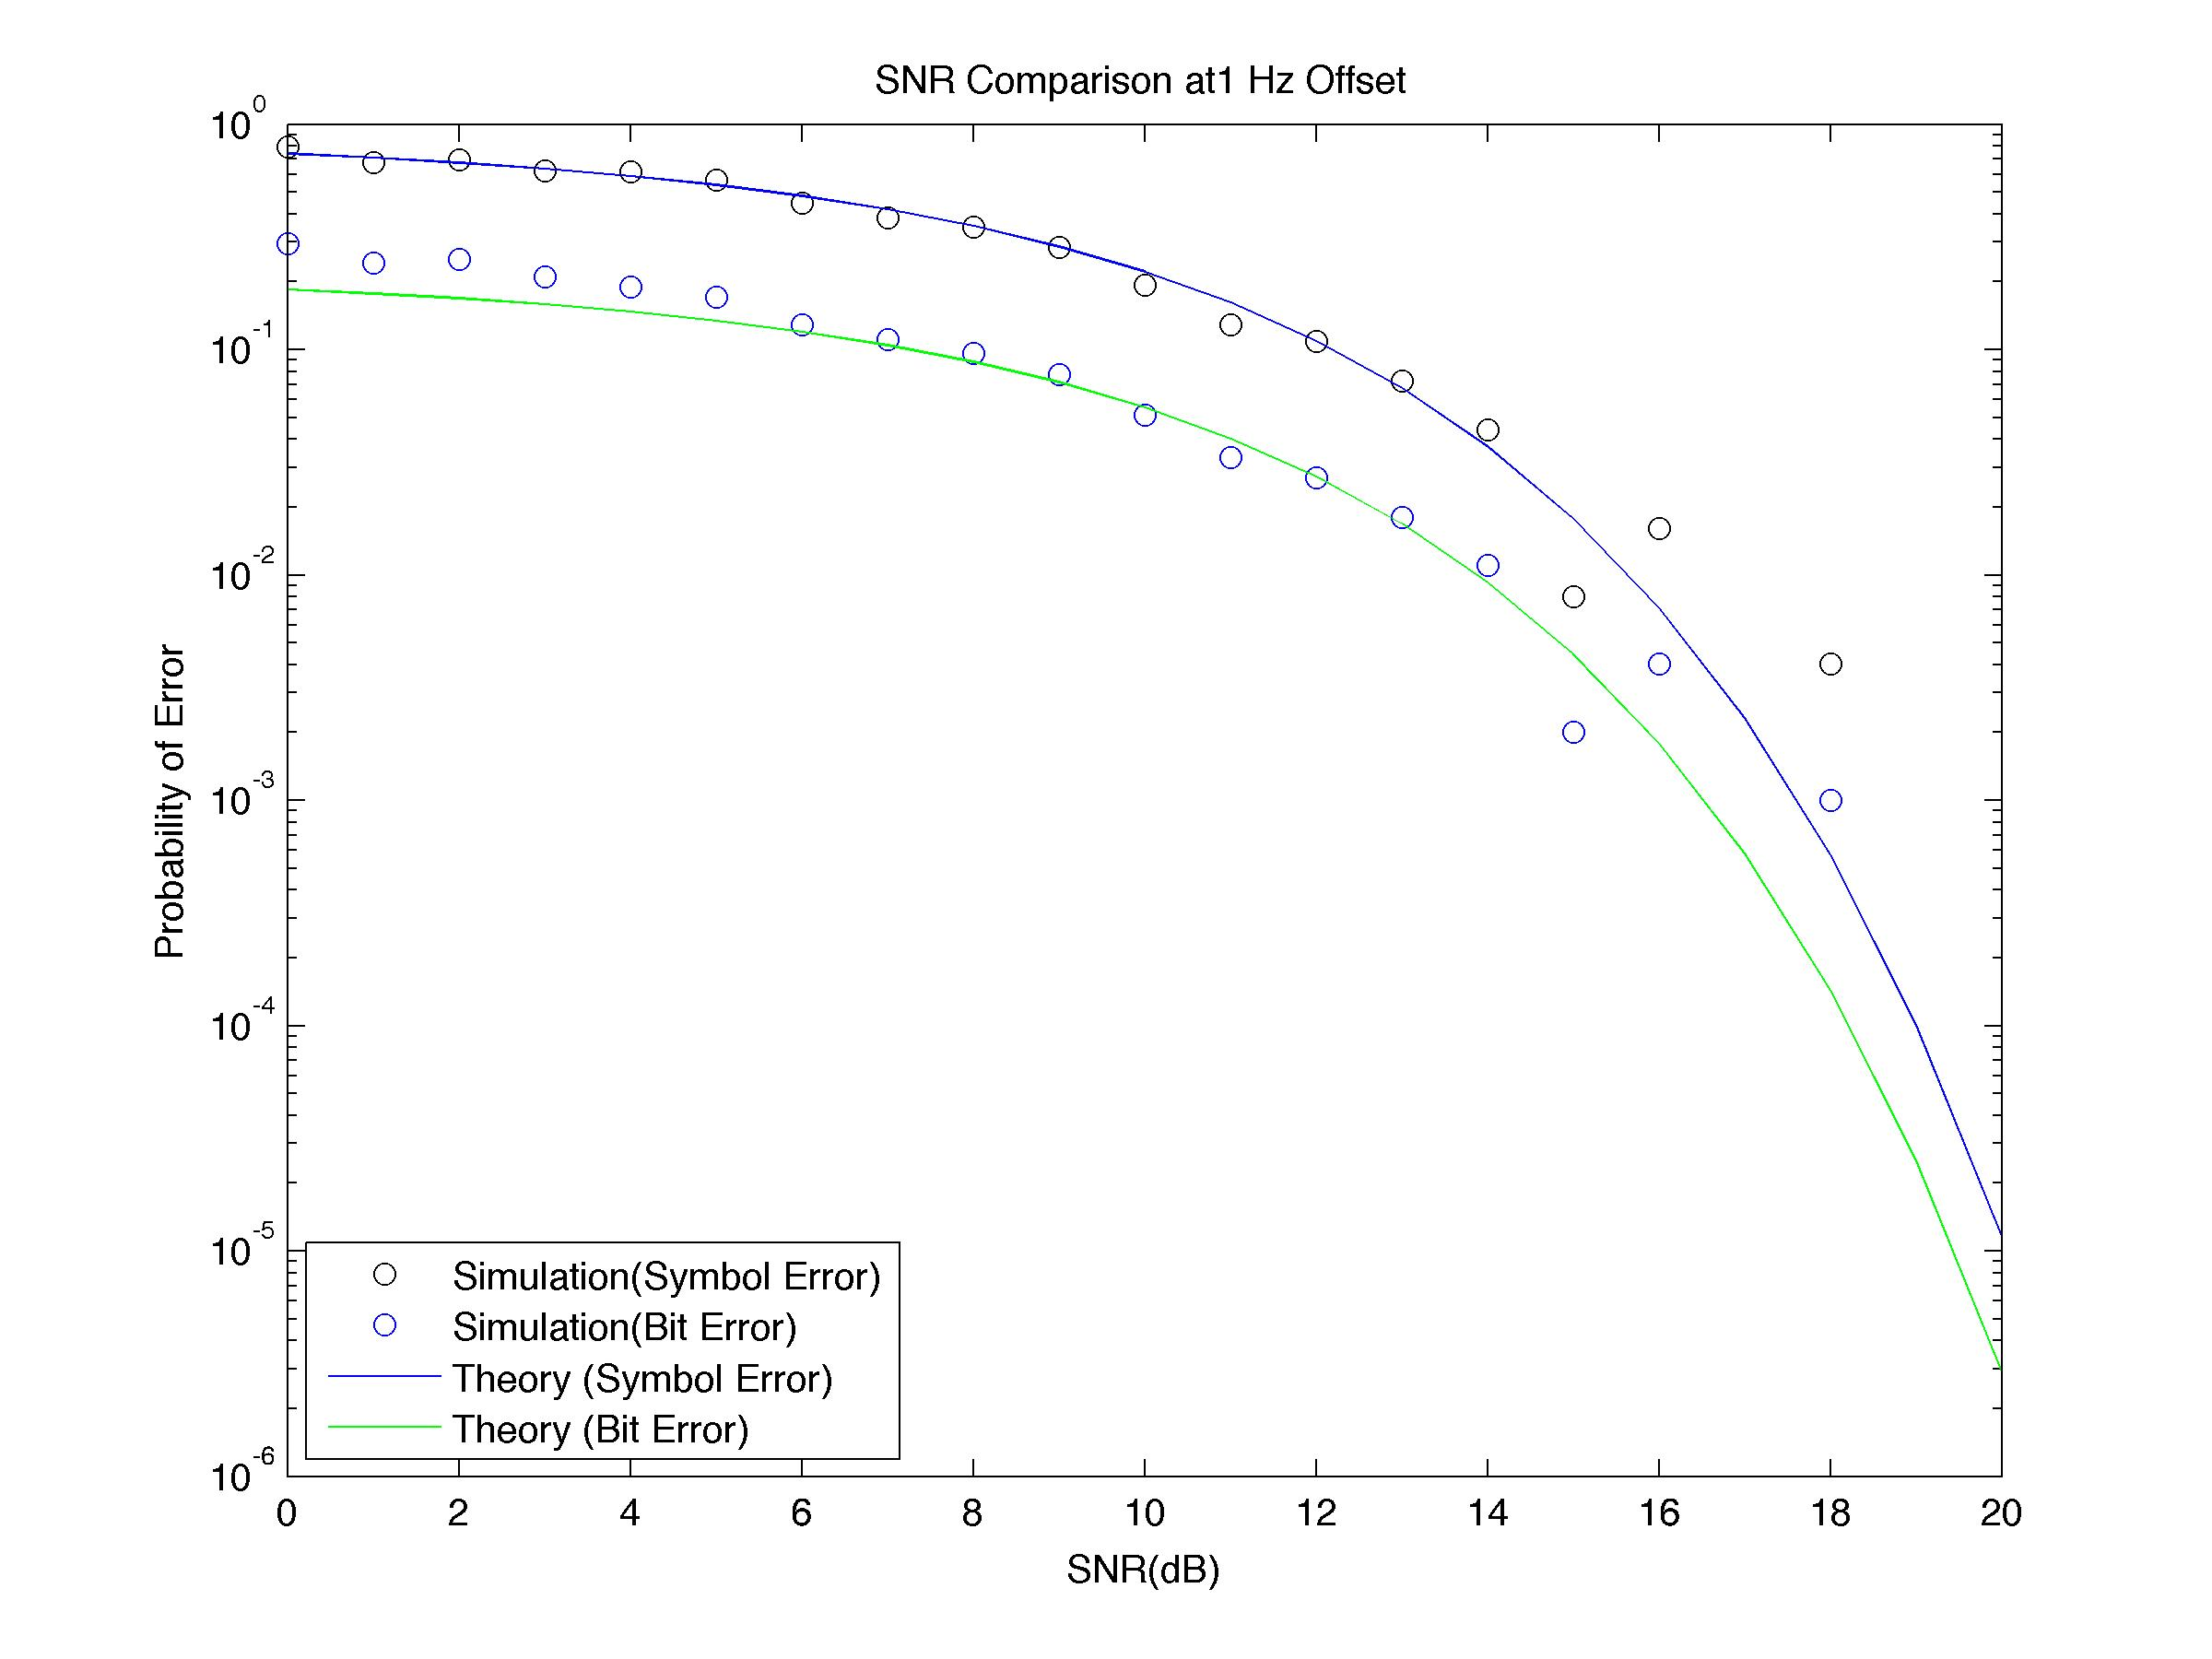
\includegraphics[width=1.3\textwidth]{qam16SNRfo3.jpg}
\caption{16-QAM Theoretical and Experimental error rates versus different SNR levels at a frequency offset of 1 Hz}
\end{figure}

\begin{figure}[H]
\centering
\hspace*{-2cm}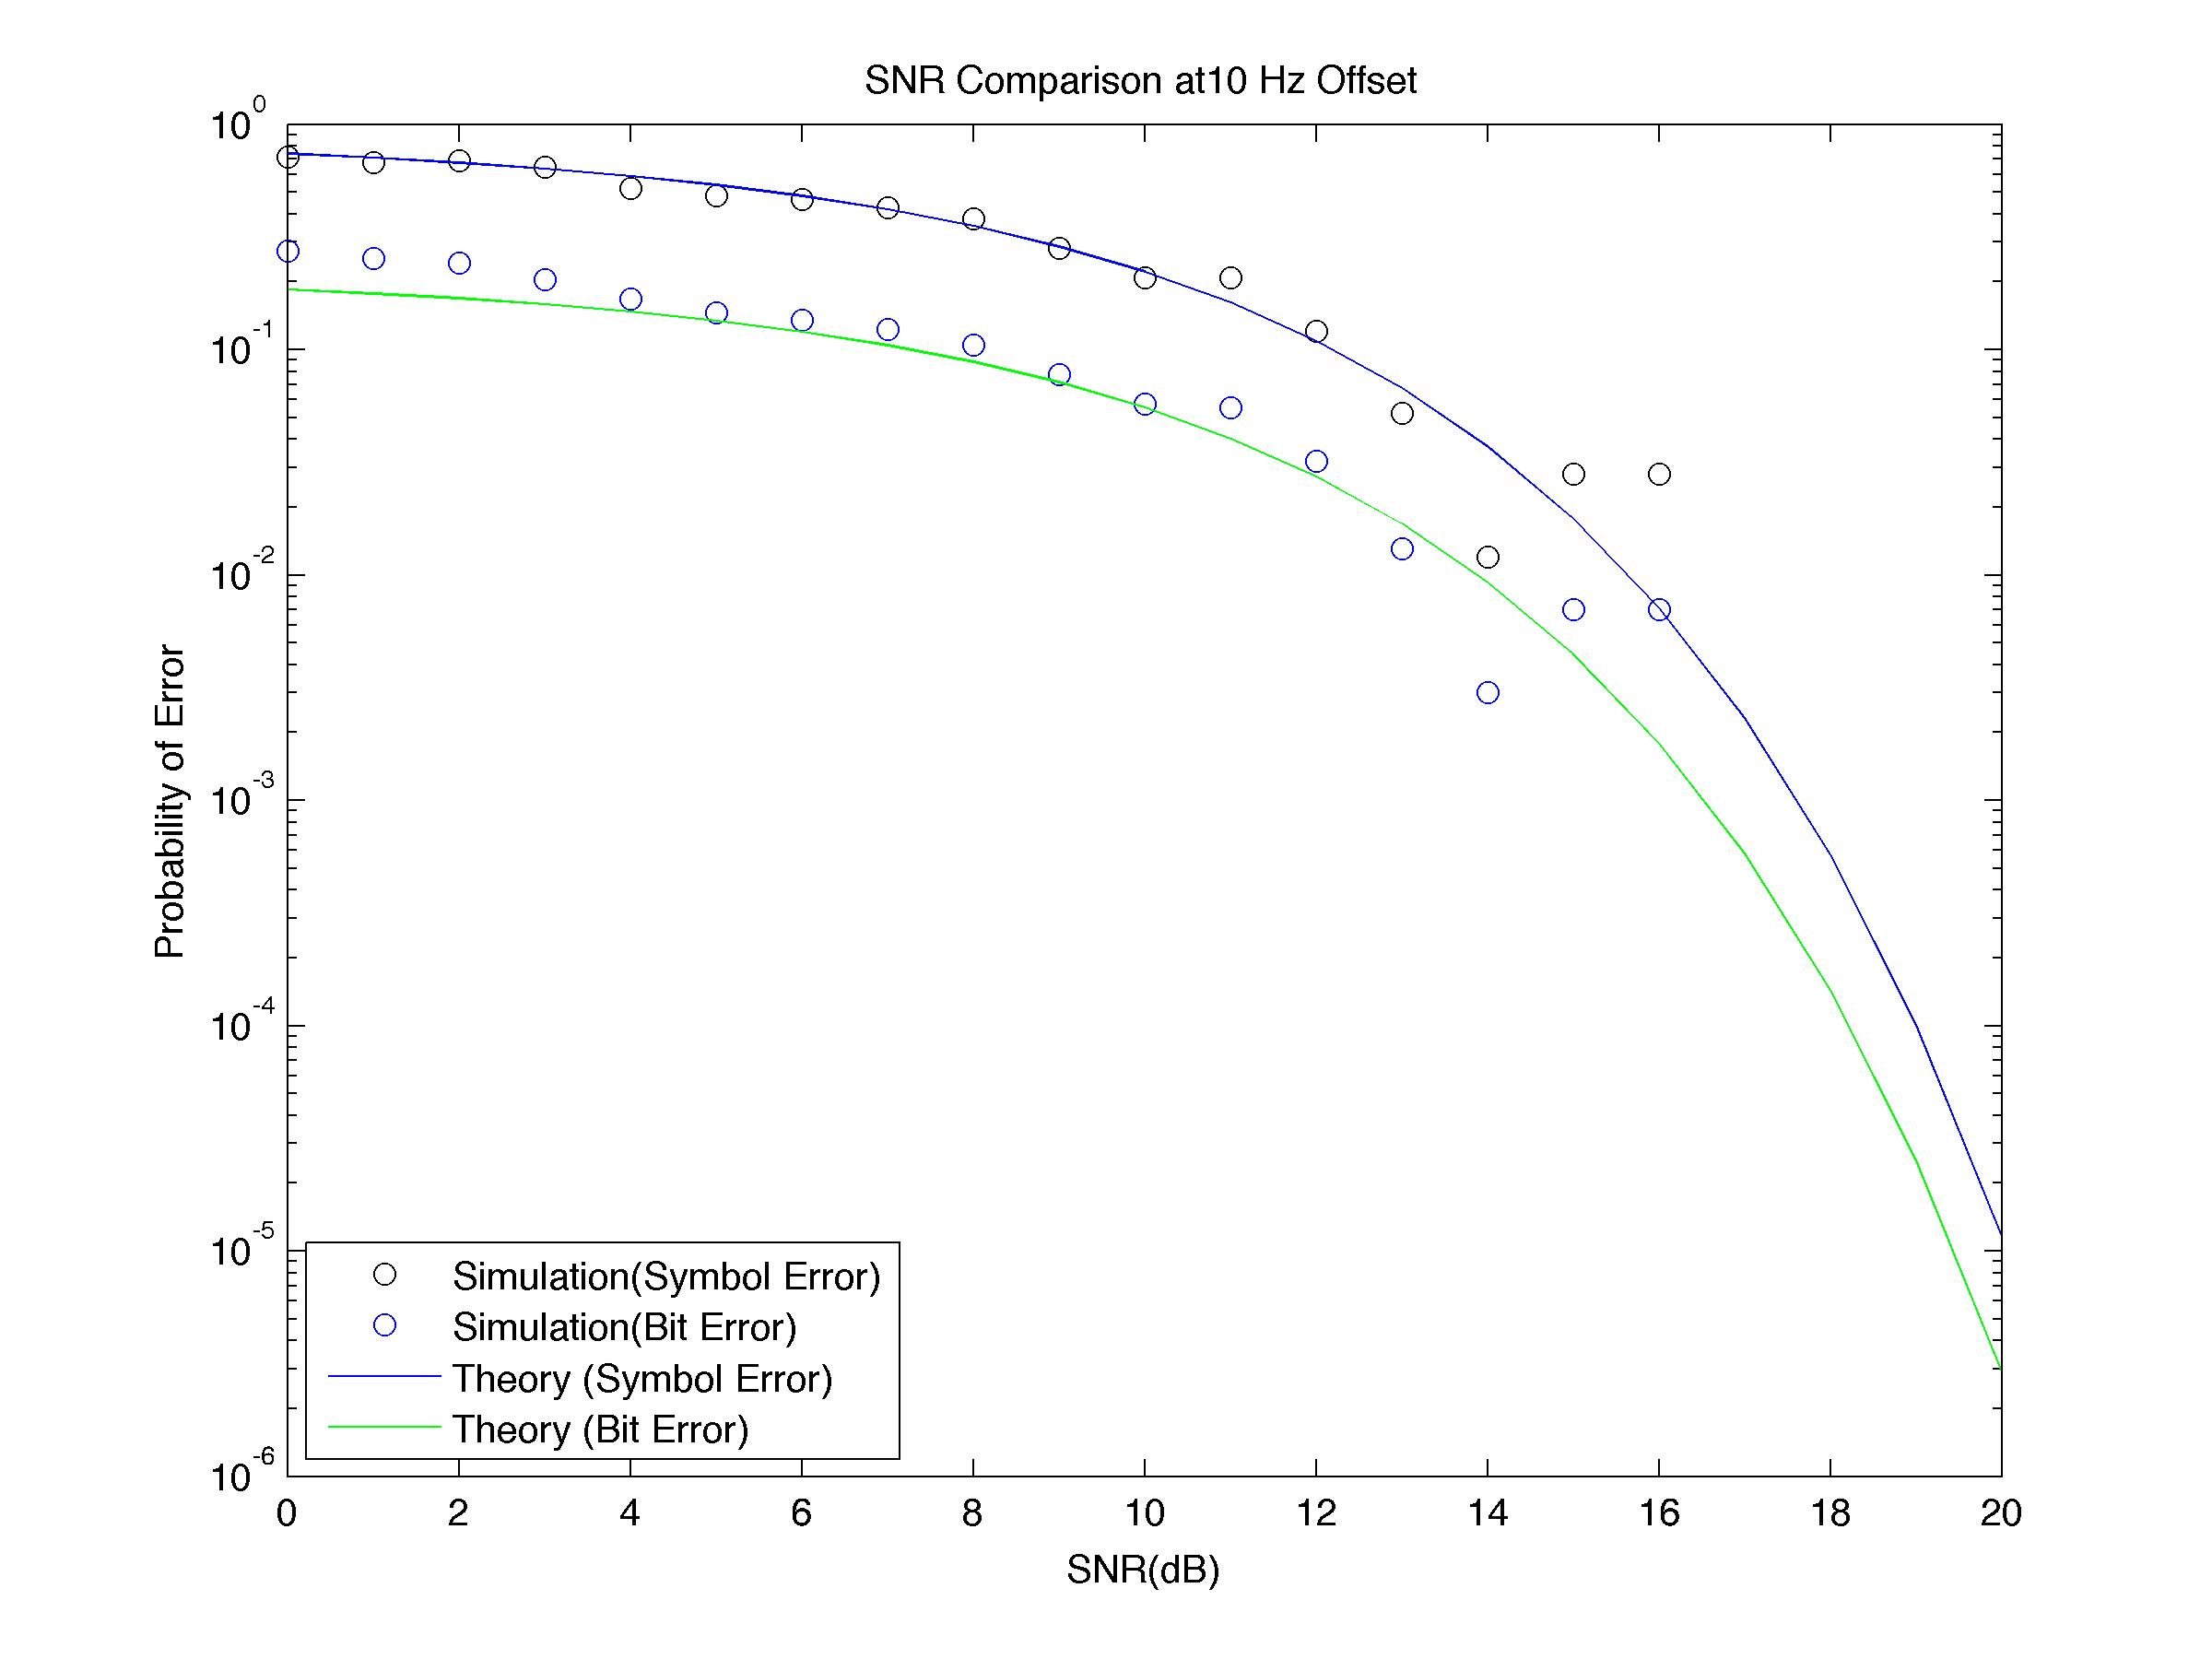
\includegraphics[width=1.3\textwidth]{qam16SNRfo4.jpg}
\caption{16-QAM Theoretical and Experimental error rates versus different SNR levels at a frequency offset of 10 Hz}
\end{figure}

\subsubsection{64-QAM with Frequency Offset}
\begin{figure}[H]
\centering
\hspace*{-2cm}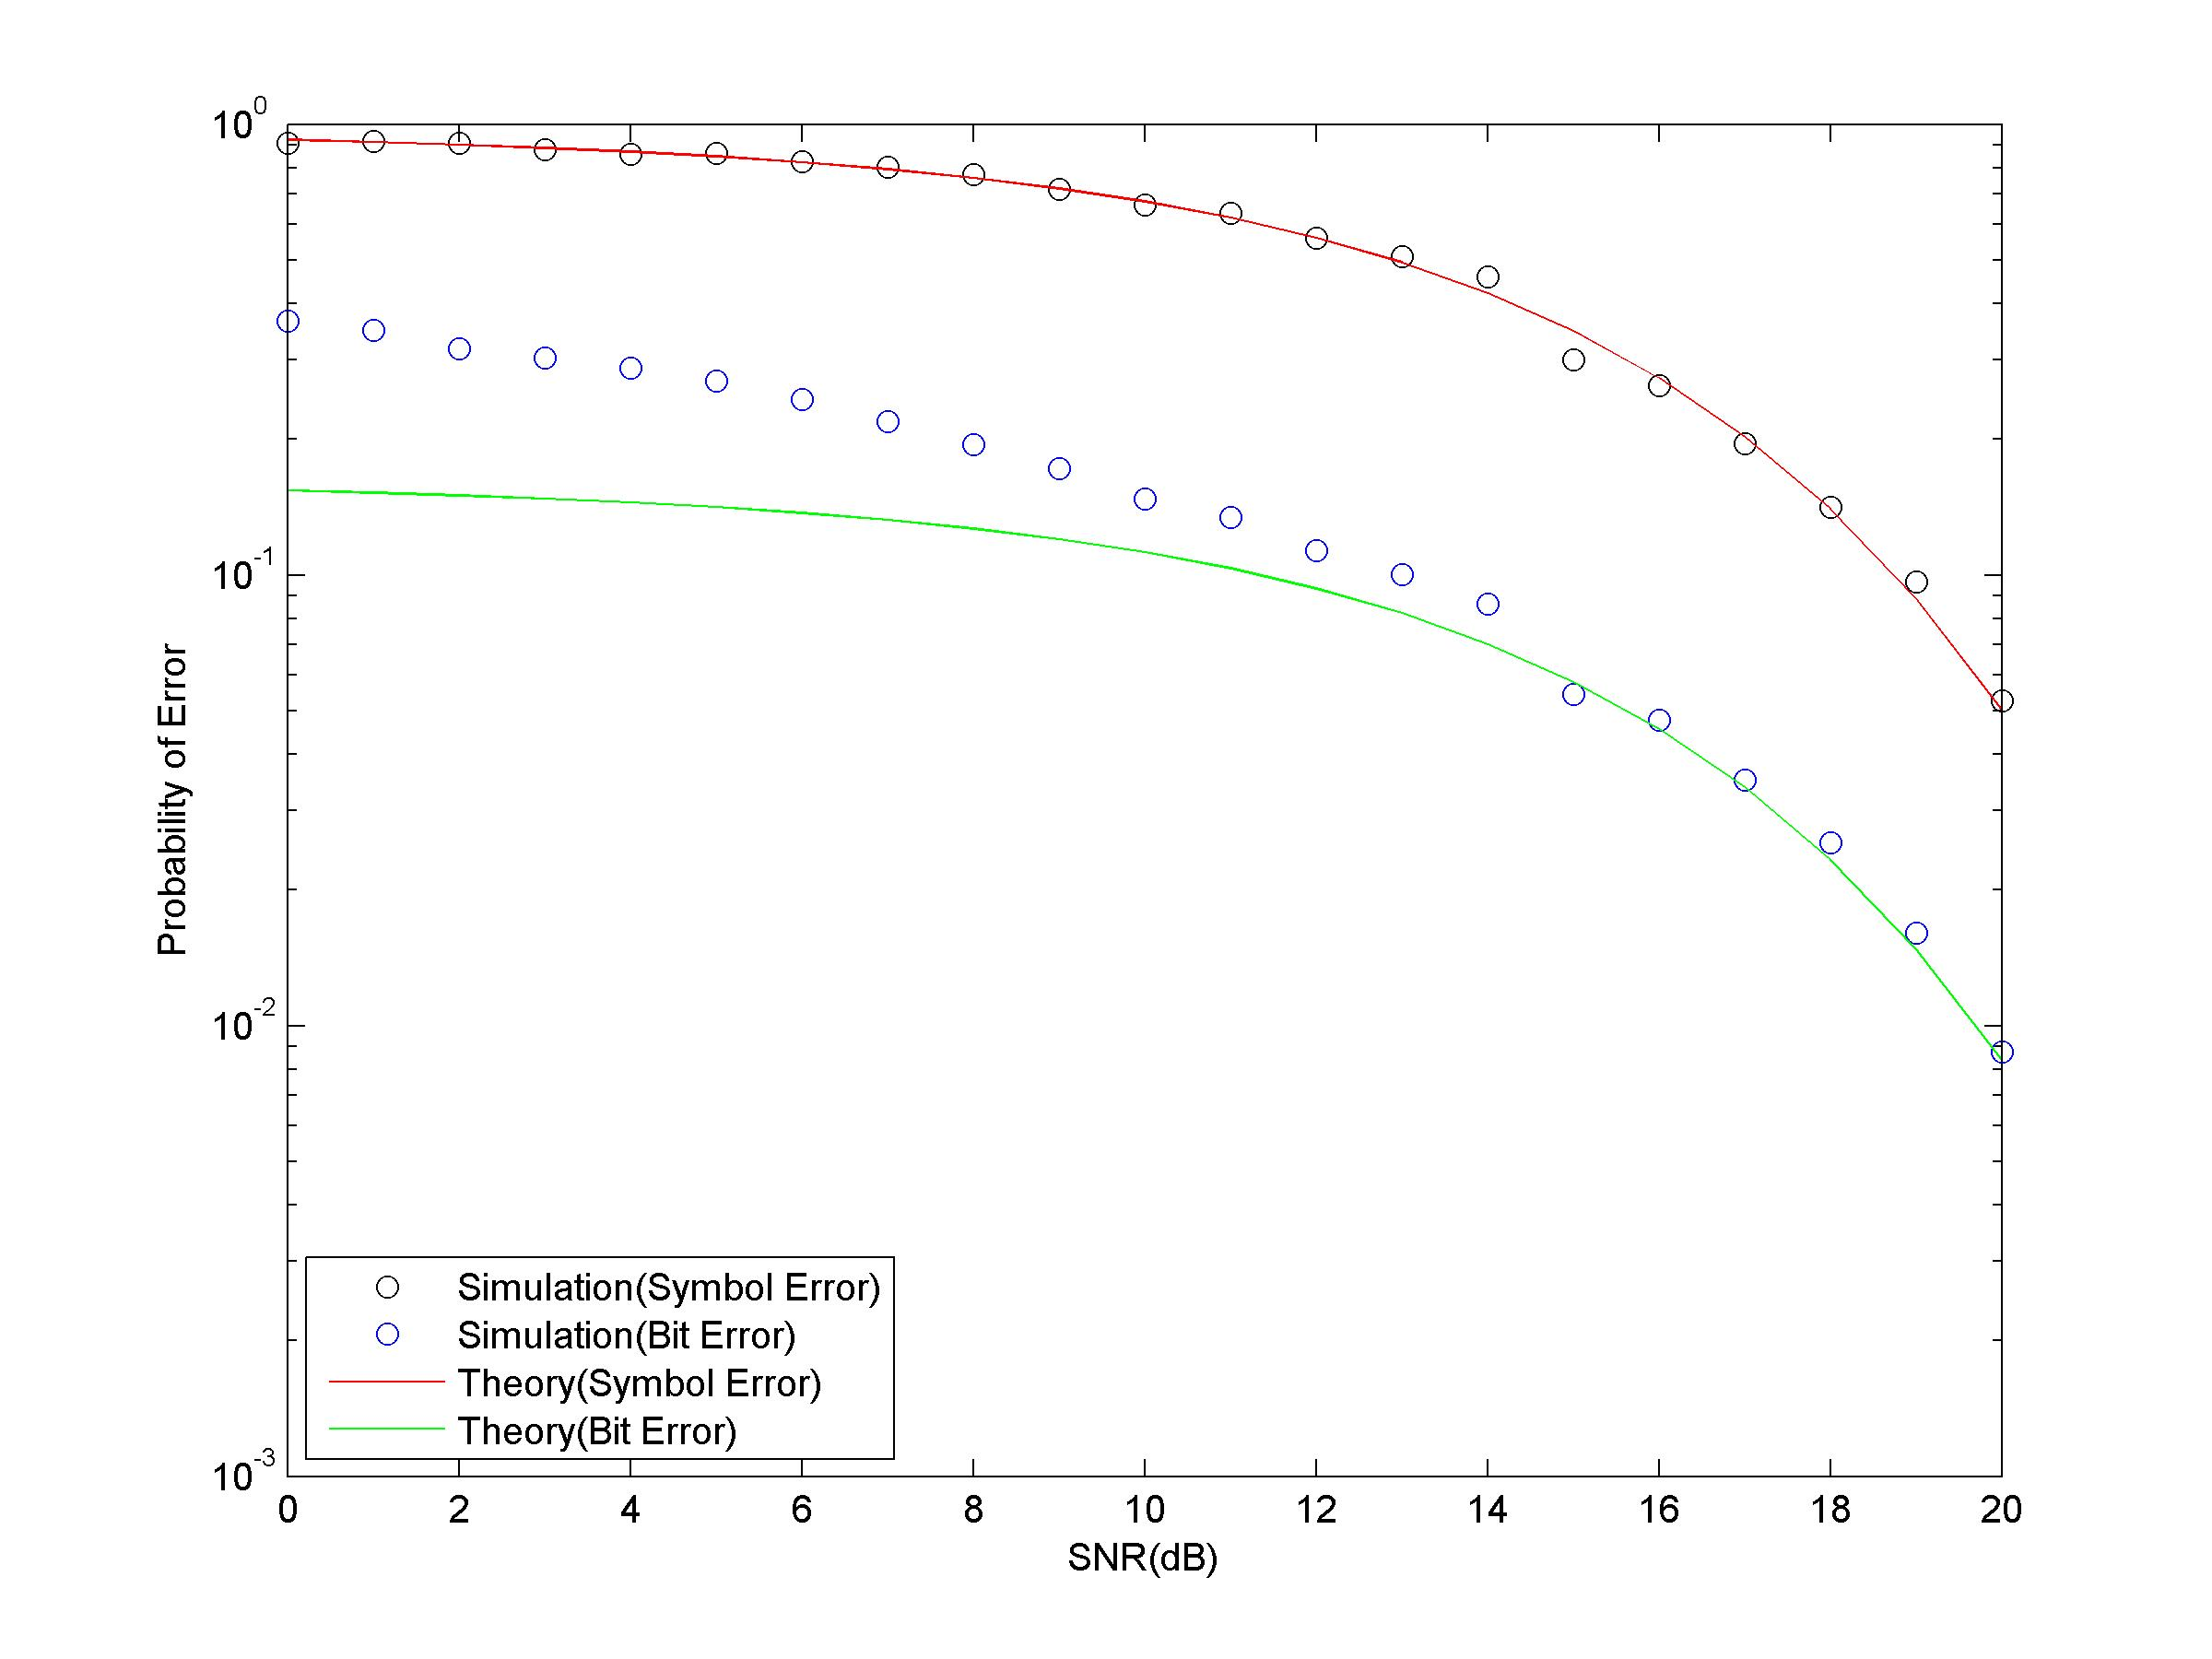
\includegraphics[width=1.3\textwidth]{qam64SNRfo1.jpg}
\caption{64-QAM Theoretical and Experimental error rates versus different SNR levels at a frequency offset of 0.01 Hz}
\end{figure}

\begin{figure}[H]
\centering
\hspace*{-2cm}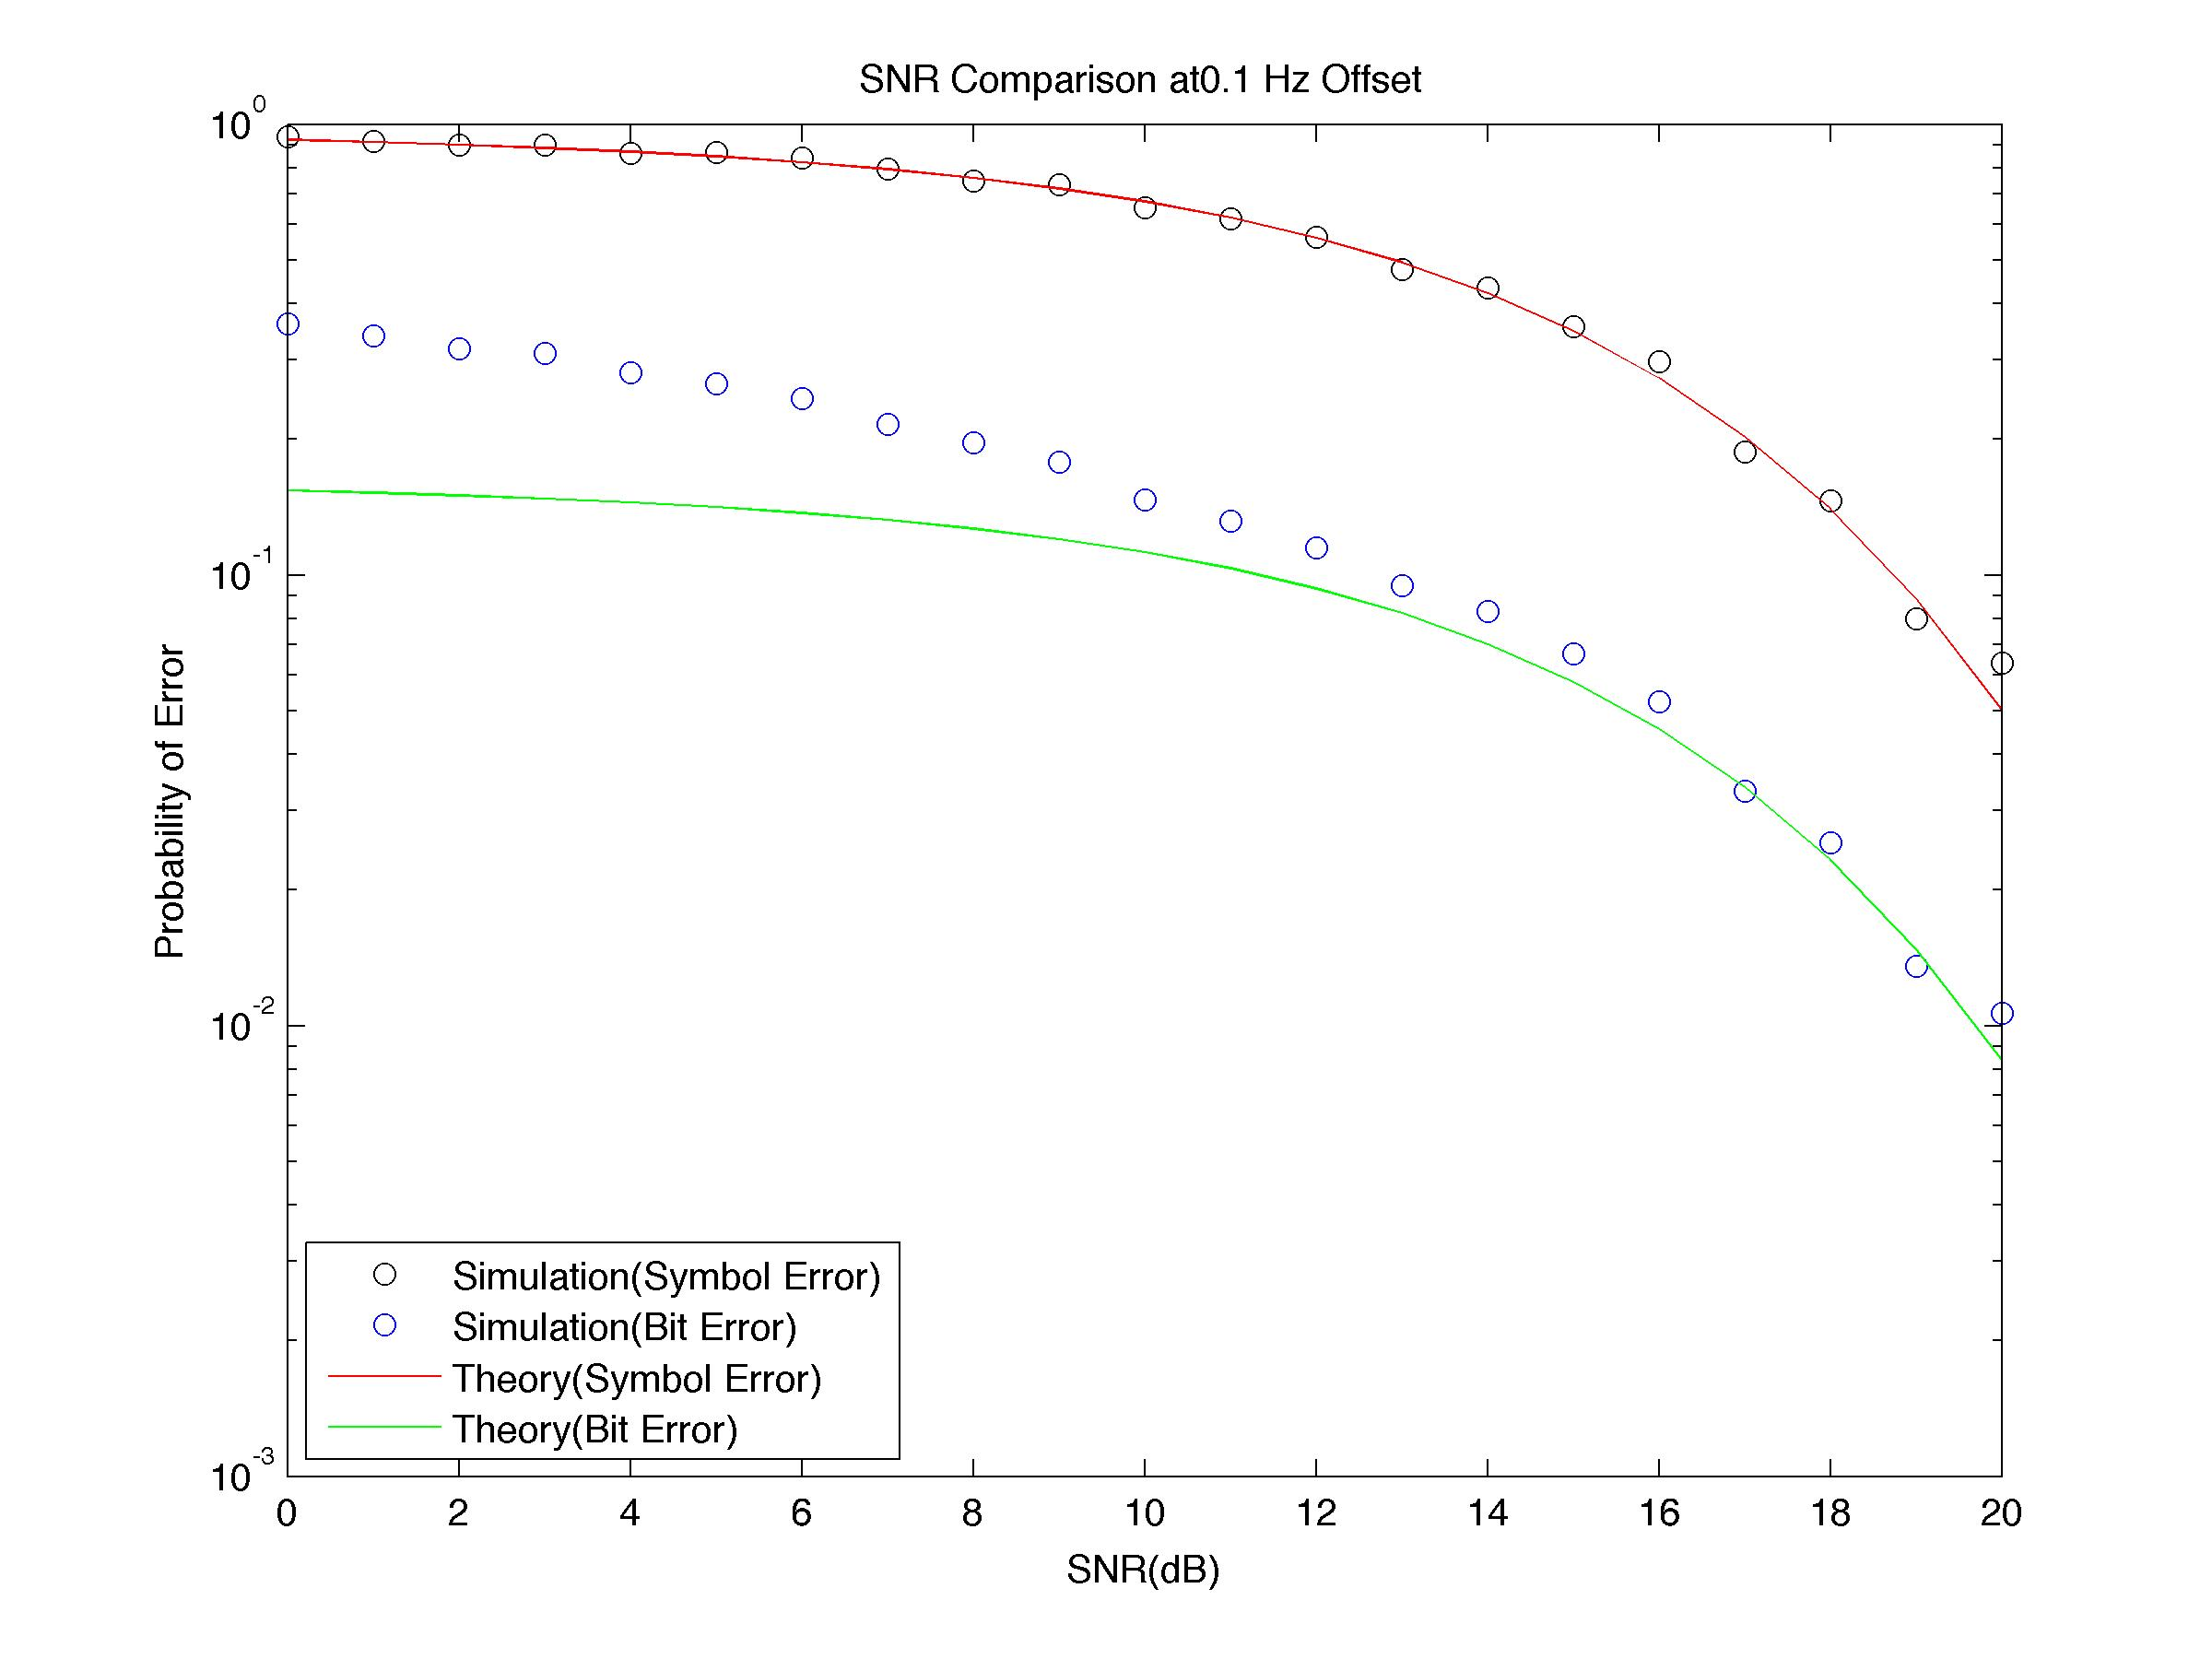
\includegraphics[width=1.3\textwidth]{qam64SNRfo2.jpg}
\caption{64-QAM Theoretical and Experimental error rates versus different SNR levels at a frequency offset of 0.1 Hz}
\end{figure}

\begin{figure}[H]
\centering
\hspace*{-2cm}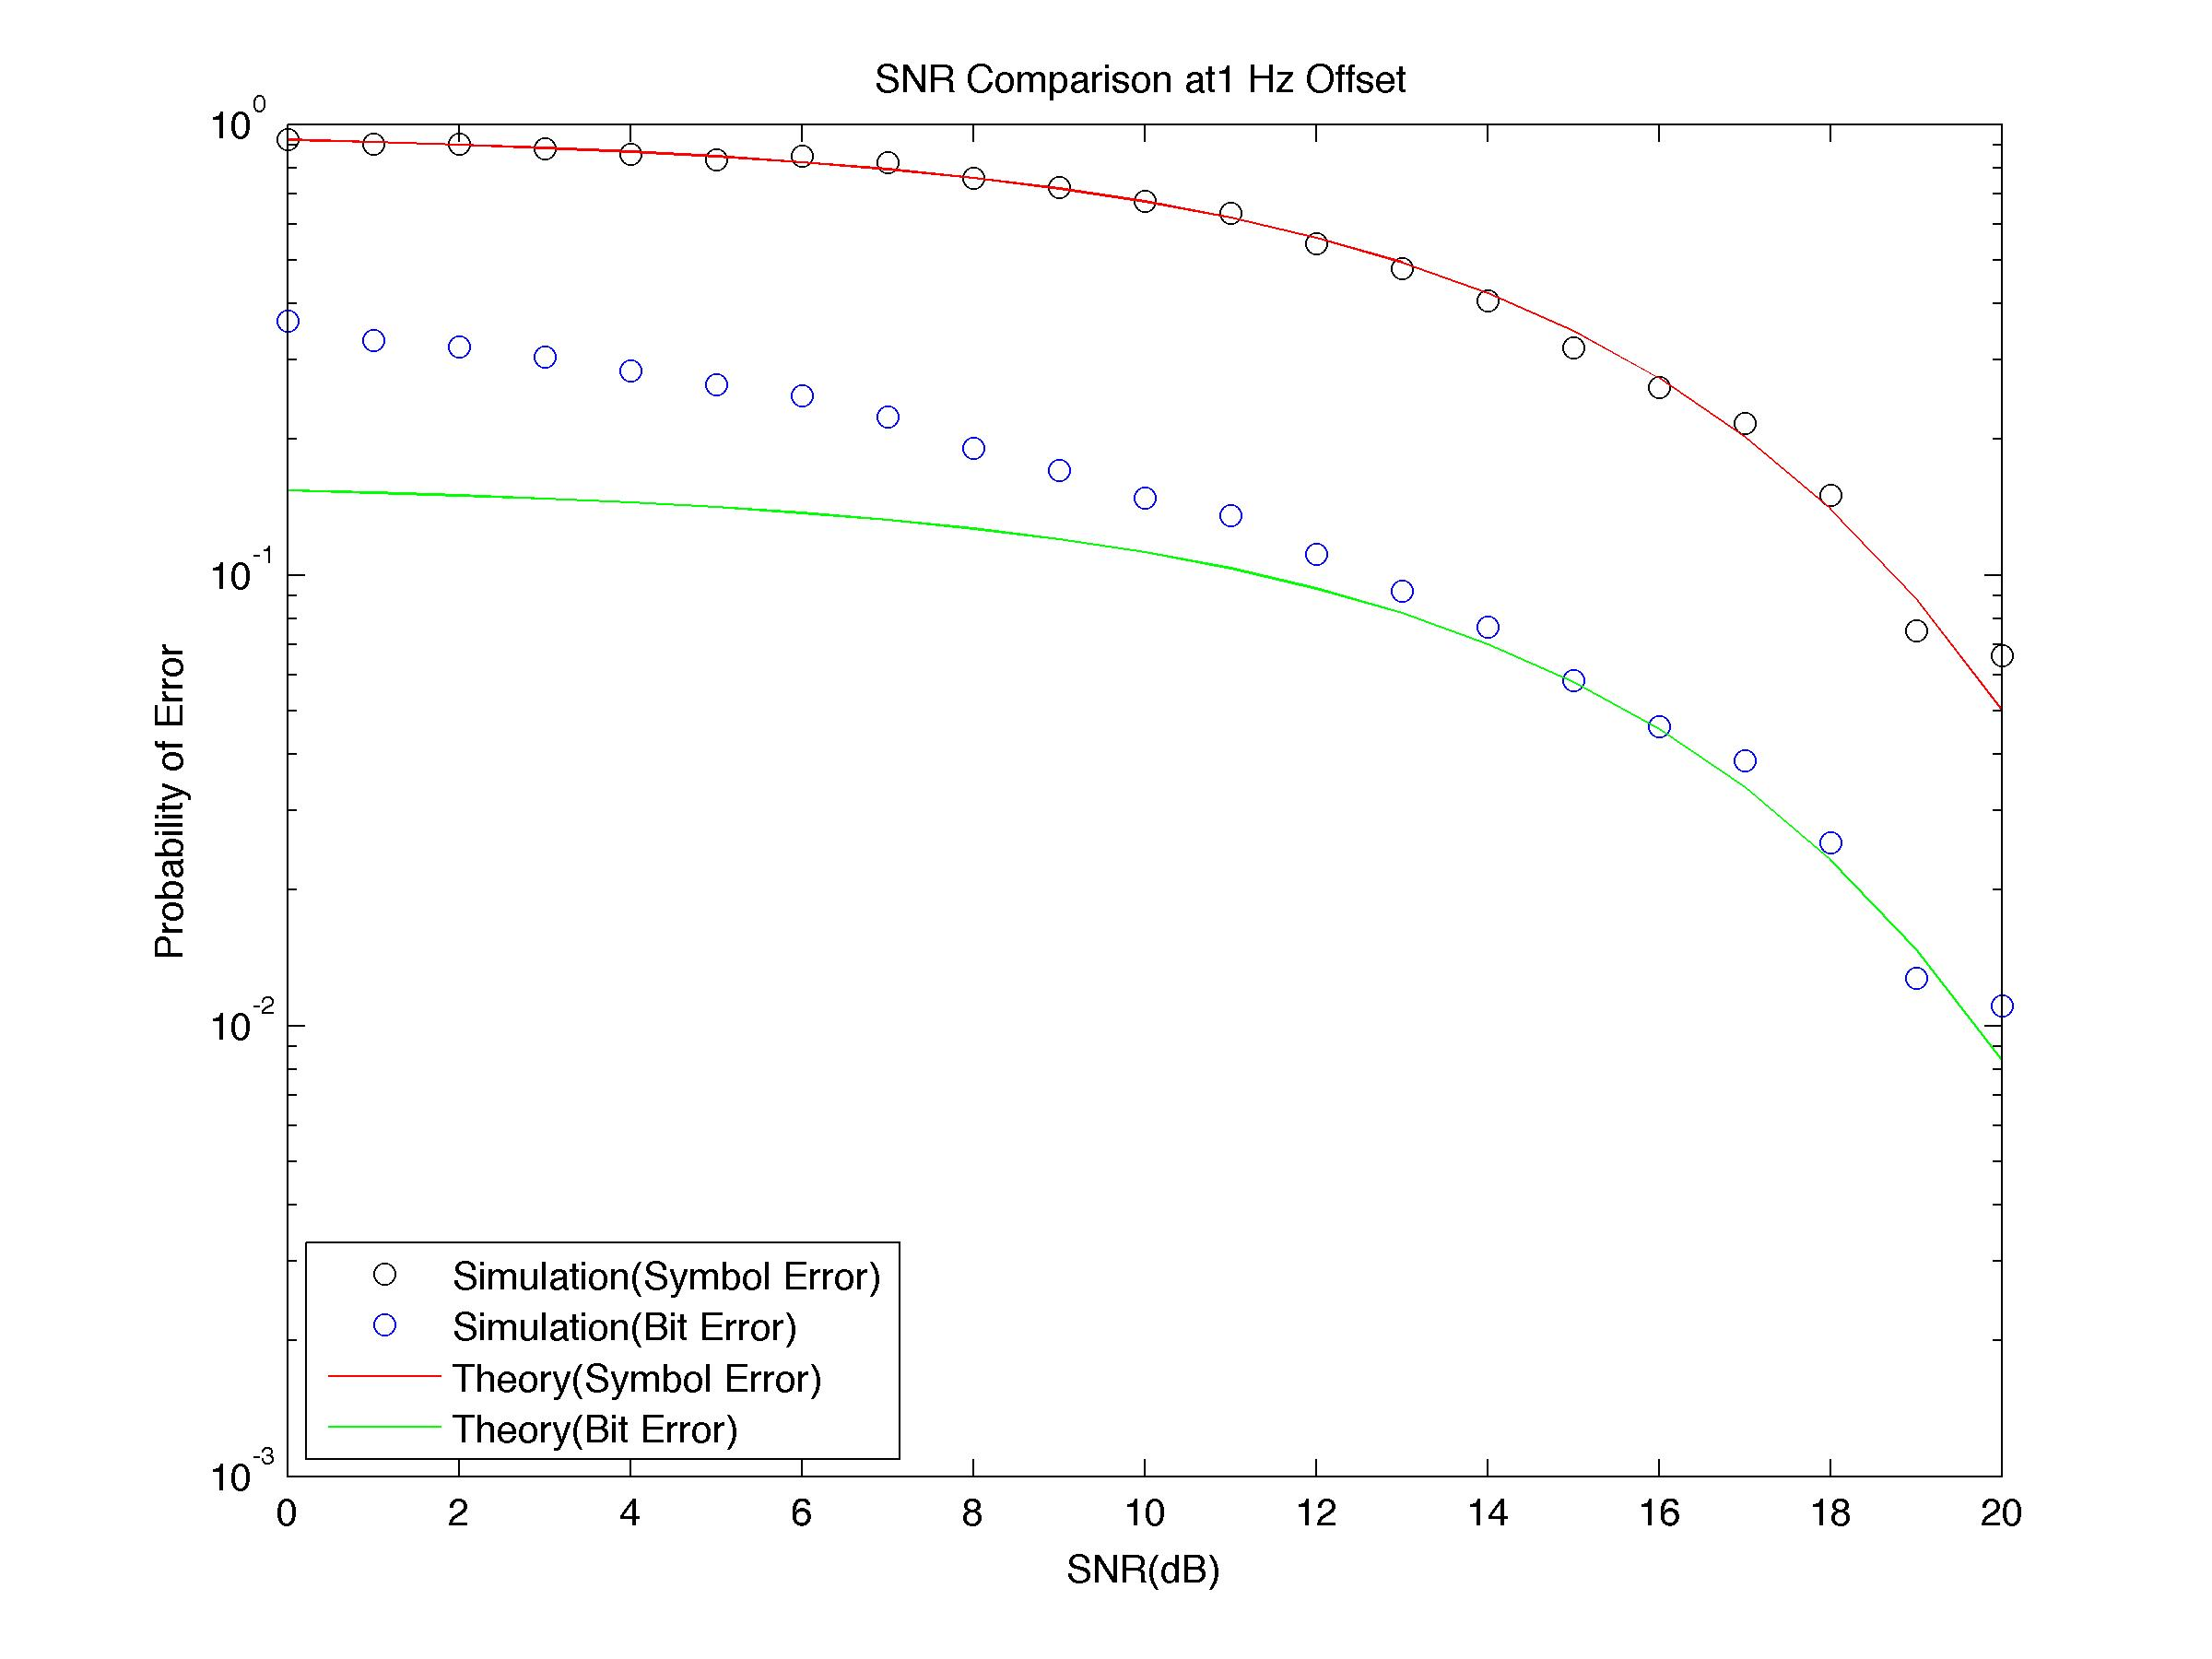
\includegraphics[width=1.3\textwidth]{qam64SNRfo3.jpg}
\caption{64-QAM Theoretical and Experimental error rates versus different SNR levels at a frequency offset of 1 Hz}
\end{figure}

\begin{figure}[H]
\centering
\hspace*{-2cm}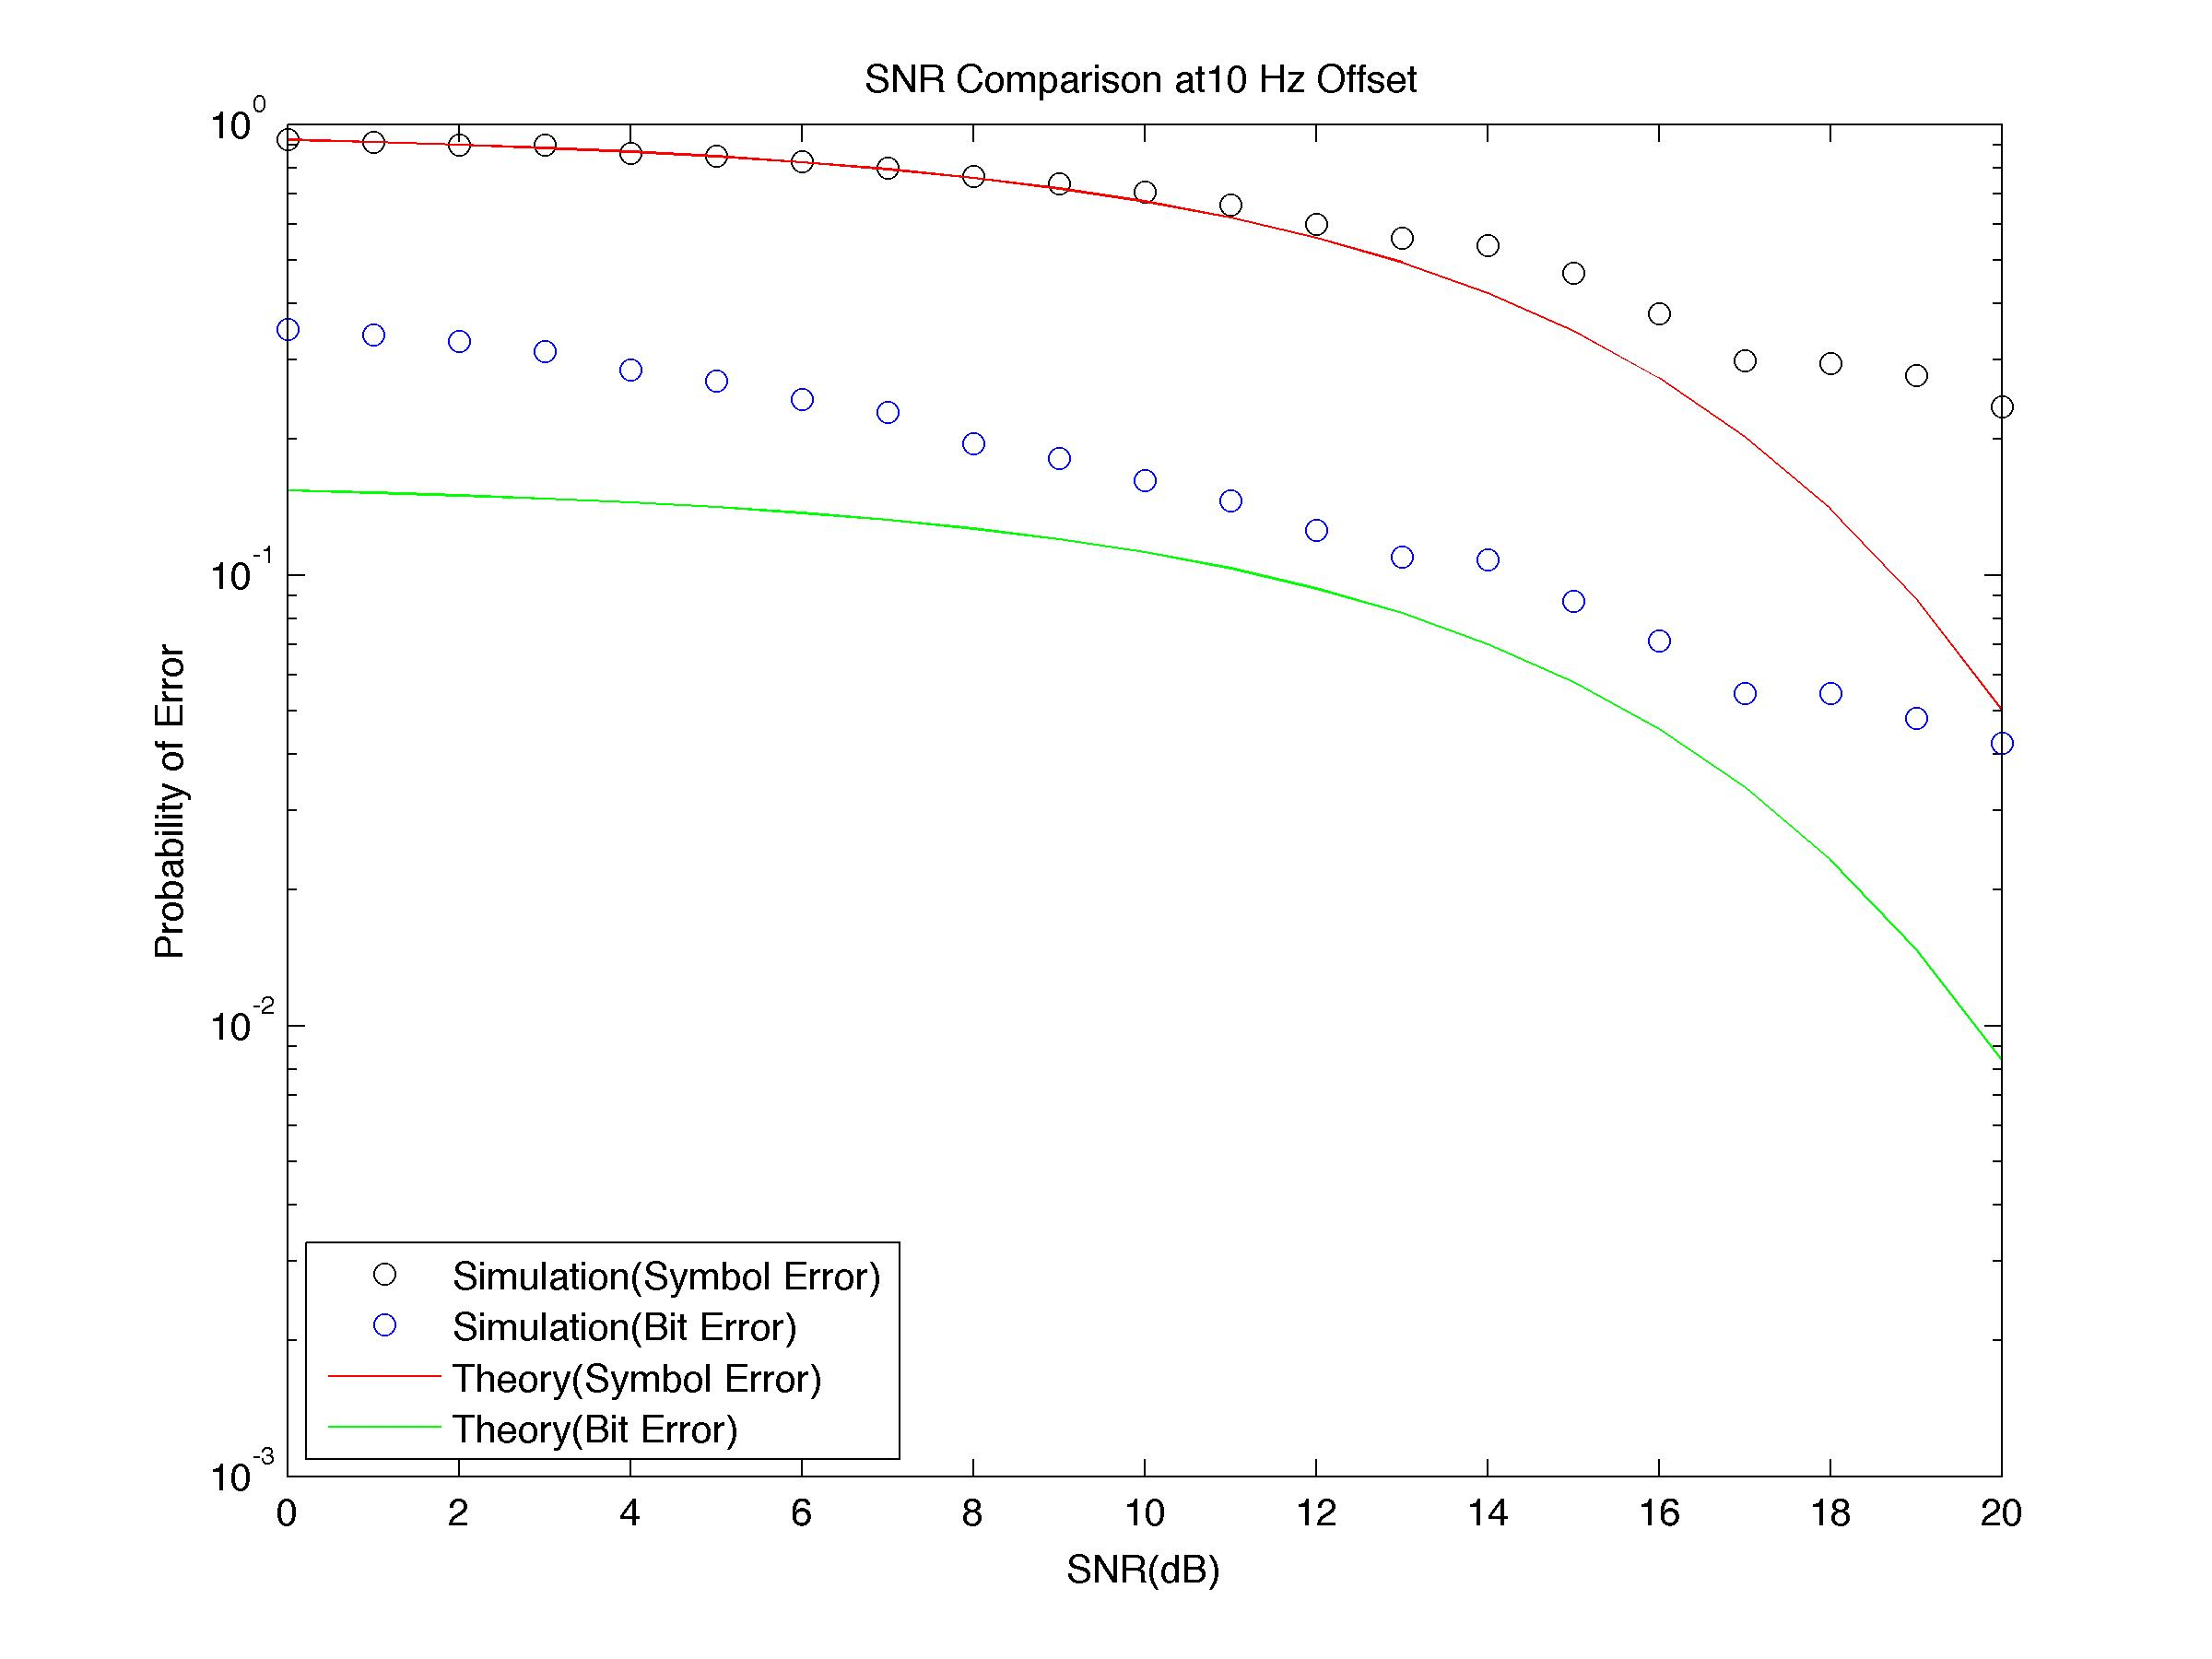
\includegraphics[width=1.3\textwidth]{qam64SNRfo4.jpg}
\caption{64-QAM Theoretical and Experimental error rates versus different SNR levels at a frequency offset of 10 Hz}
\end{figure}

\subsection{Constellation Plots for BPSK and QPSK with Frequency Offset}
In the following sections scatter plots of  BPSK and QPSK constellations are plotted at symbol/input SNRs of 3 dB, 6dB, 10dB and 20dB and frequency offsets of 0.01 Hz, 0.1 Hz, 1 Hz, 10 Hz.

\subsubsection{BPSK with Frequency Offset}
\label{sec:bpsk_freqConst}
\begin{figure}[H]
\centering
\hspace*{-2cm}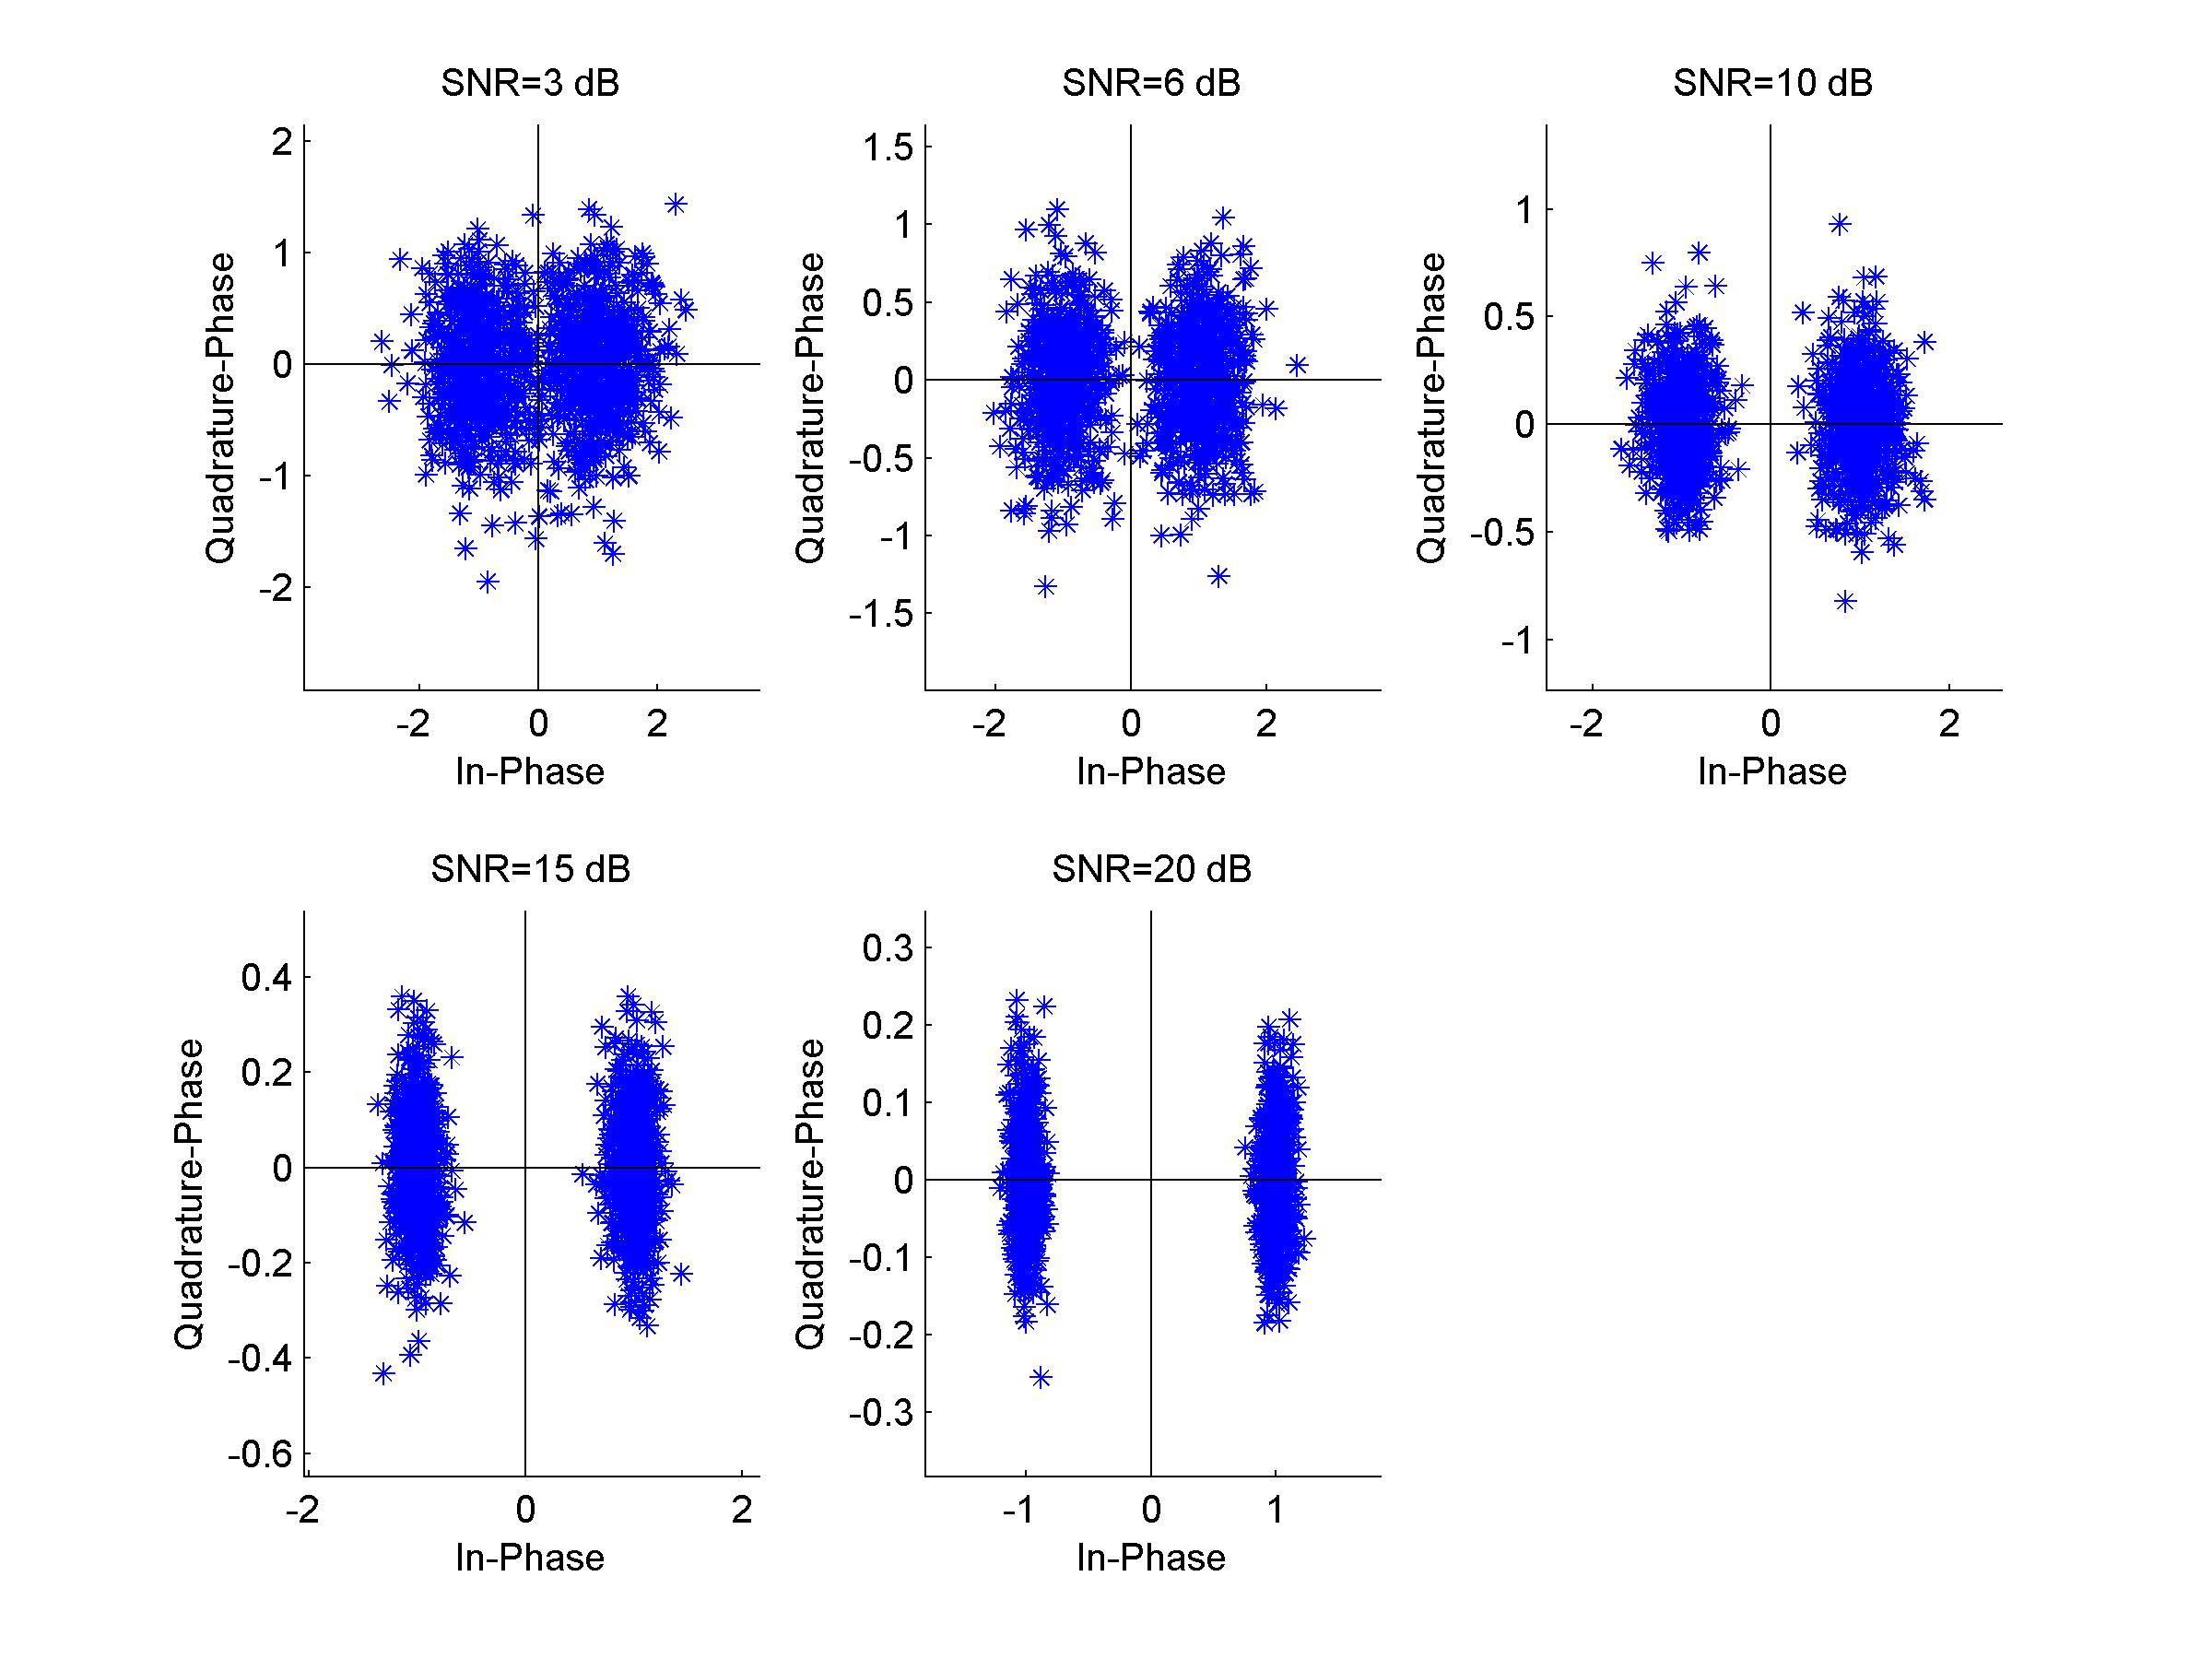
\includegraphics[width=1.3\textwidth]{bpConstfo1.jpg}
\caption{The BPSK constellation plots for different levels of SNR at a frequency offset of 0.01 Hz}
\end{figure}

\begin{figure}[H]
\centering
\hspace*{-2cm}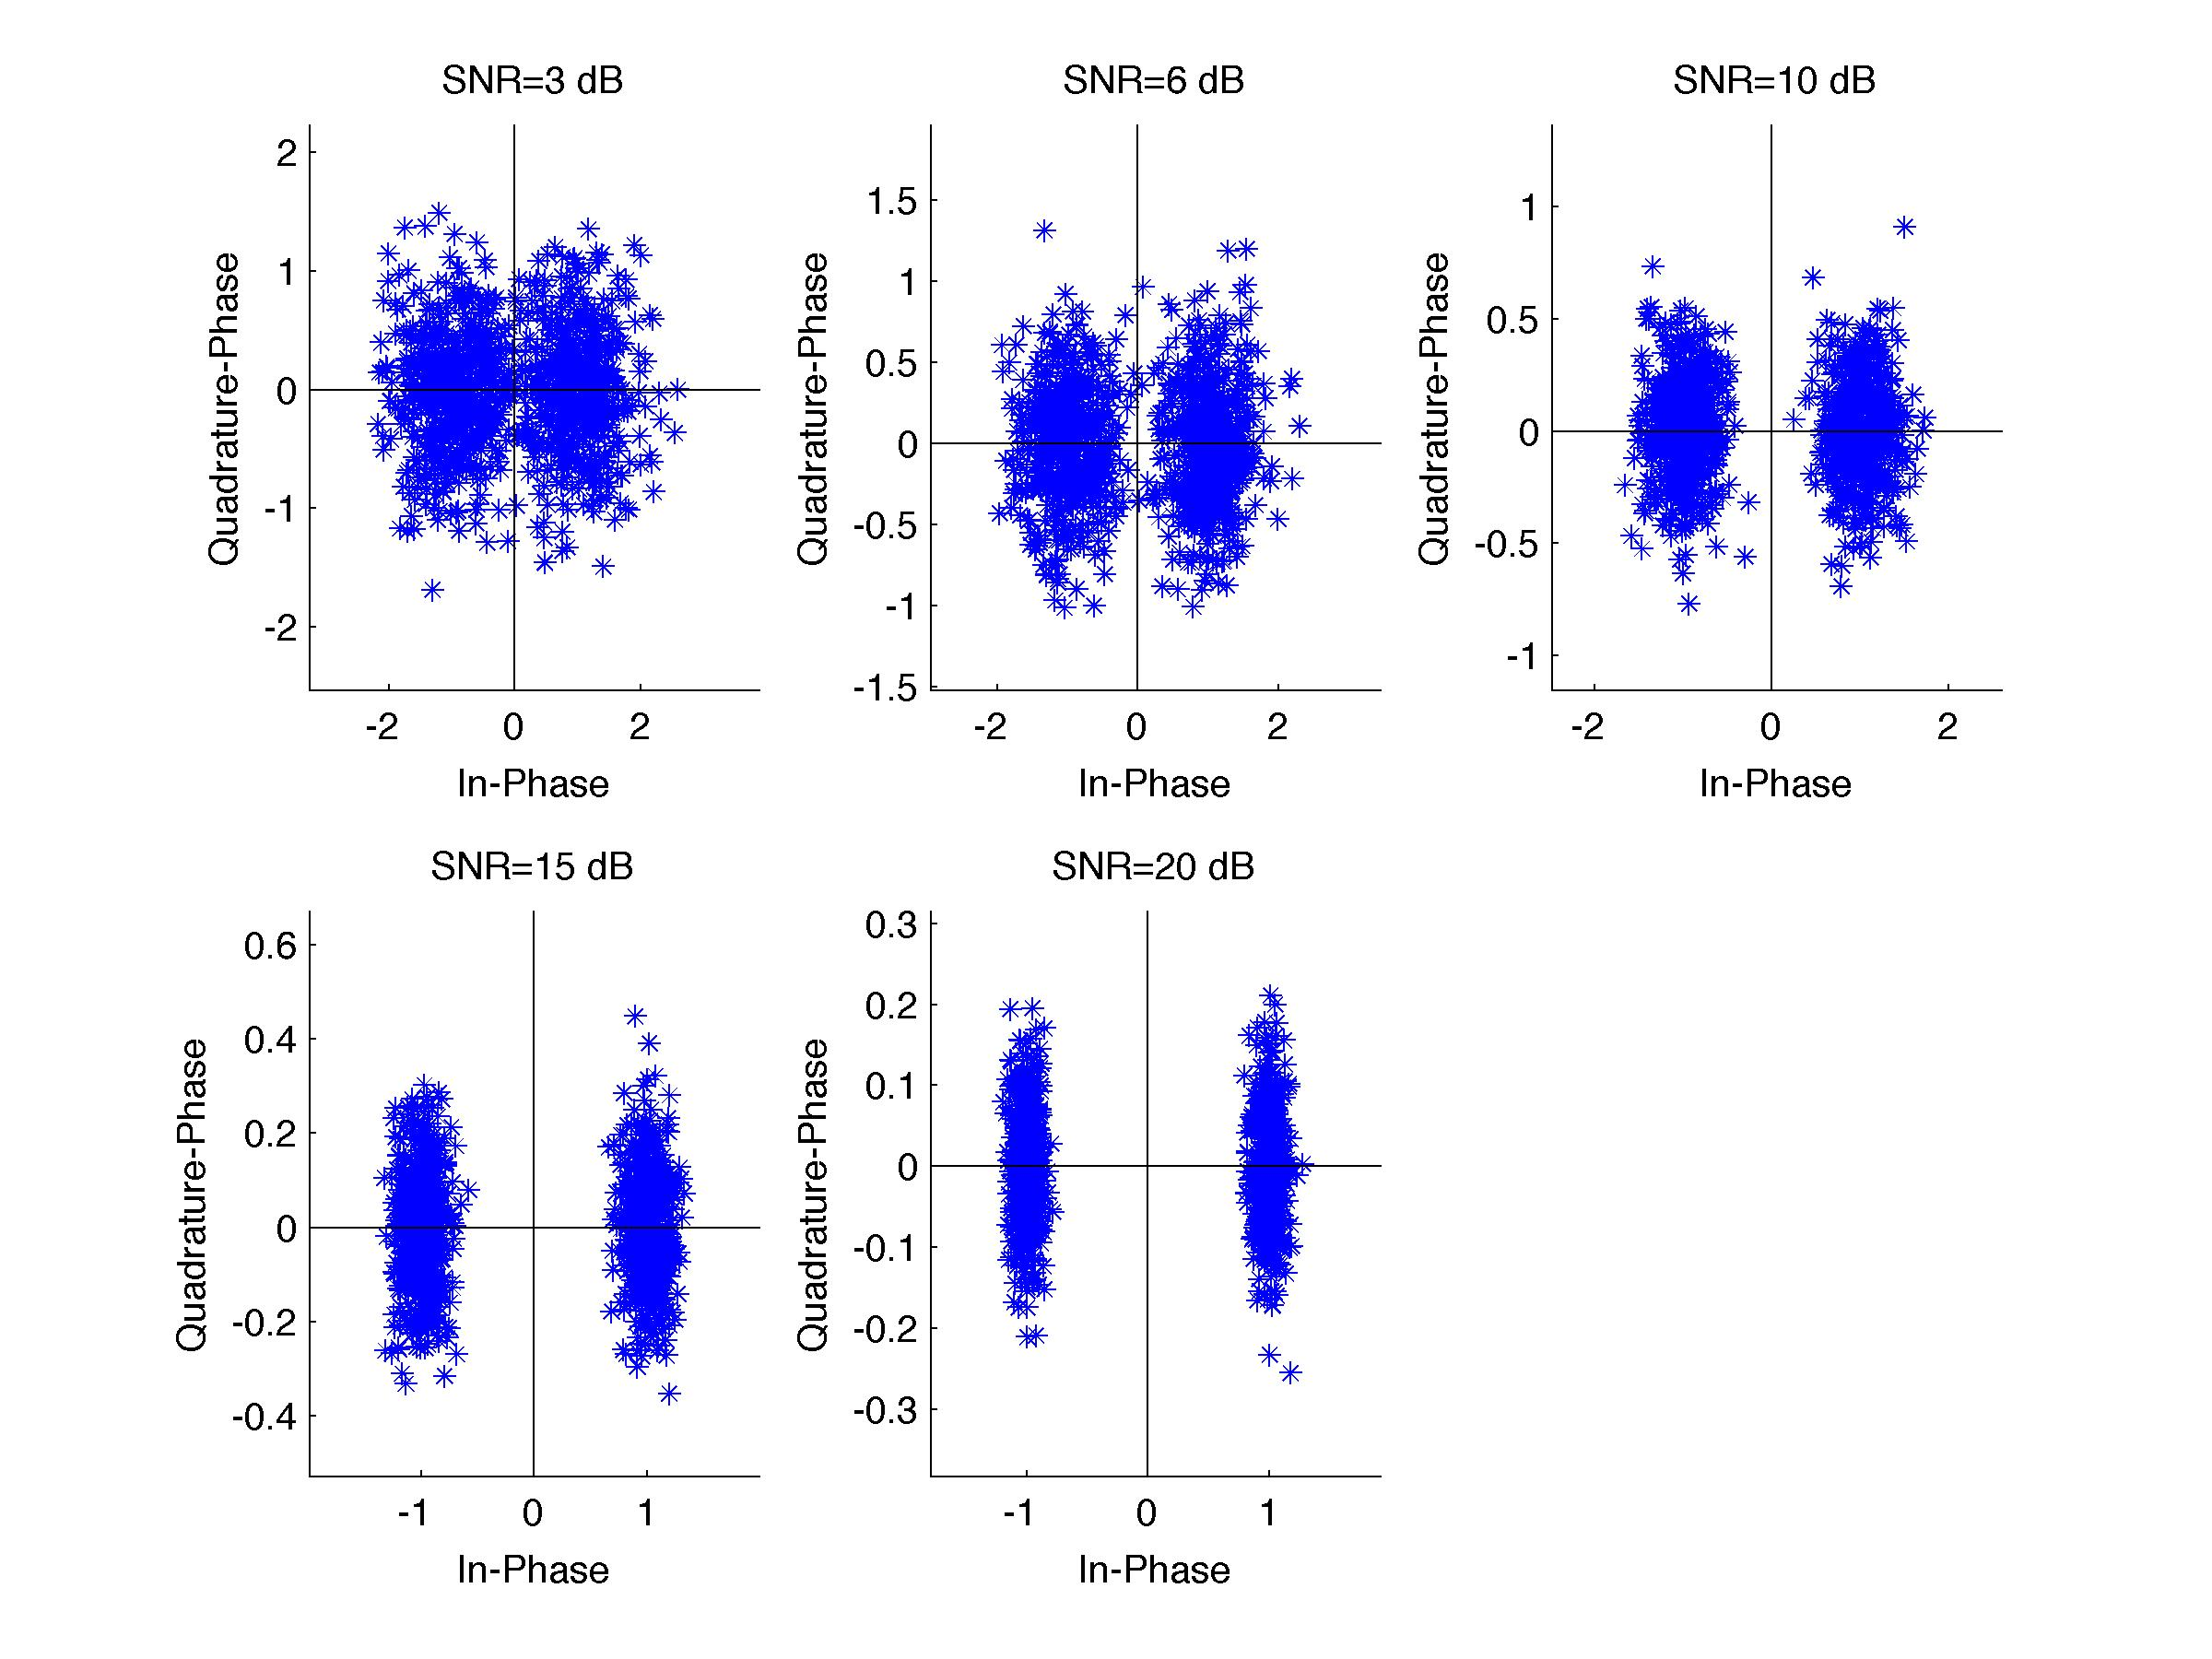
\includegraphics[width=1.3\textwidth]{bpConstfo2.jpg}
\caption{The BPSK constellation plots for different levels of SNR at a frequency offset of 0.1 Hz}
\end{figure}

\begin{figure}[H]
\centering
\hspace*{-2cm}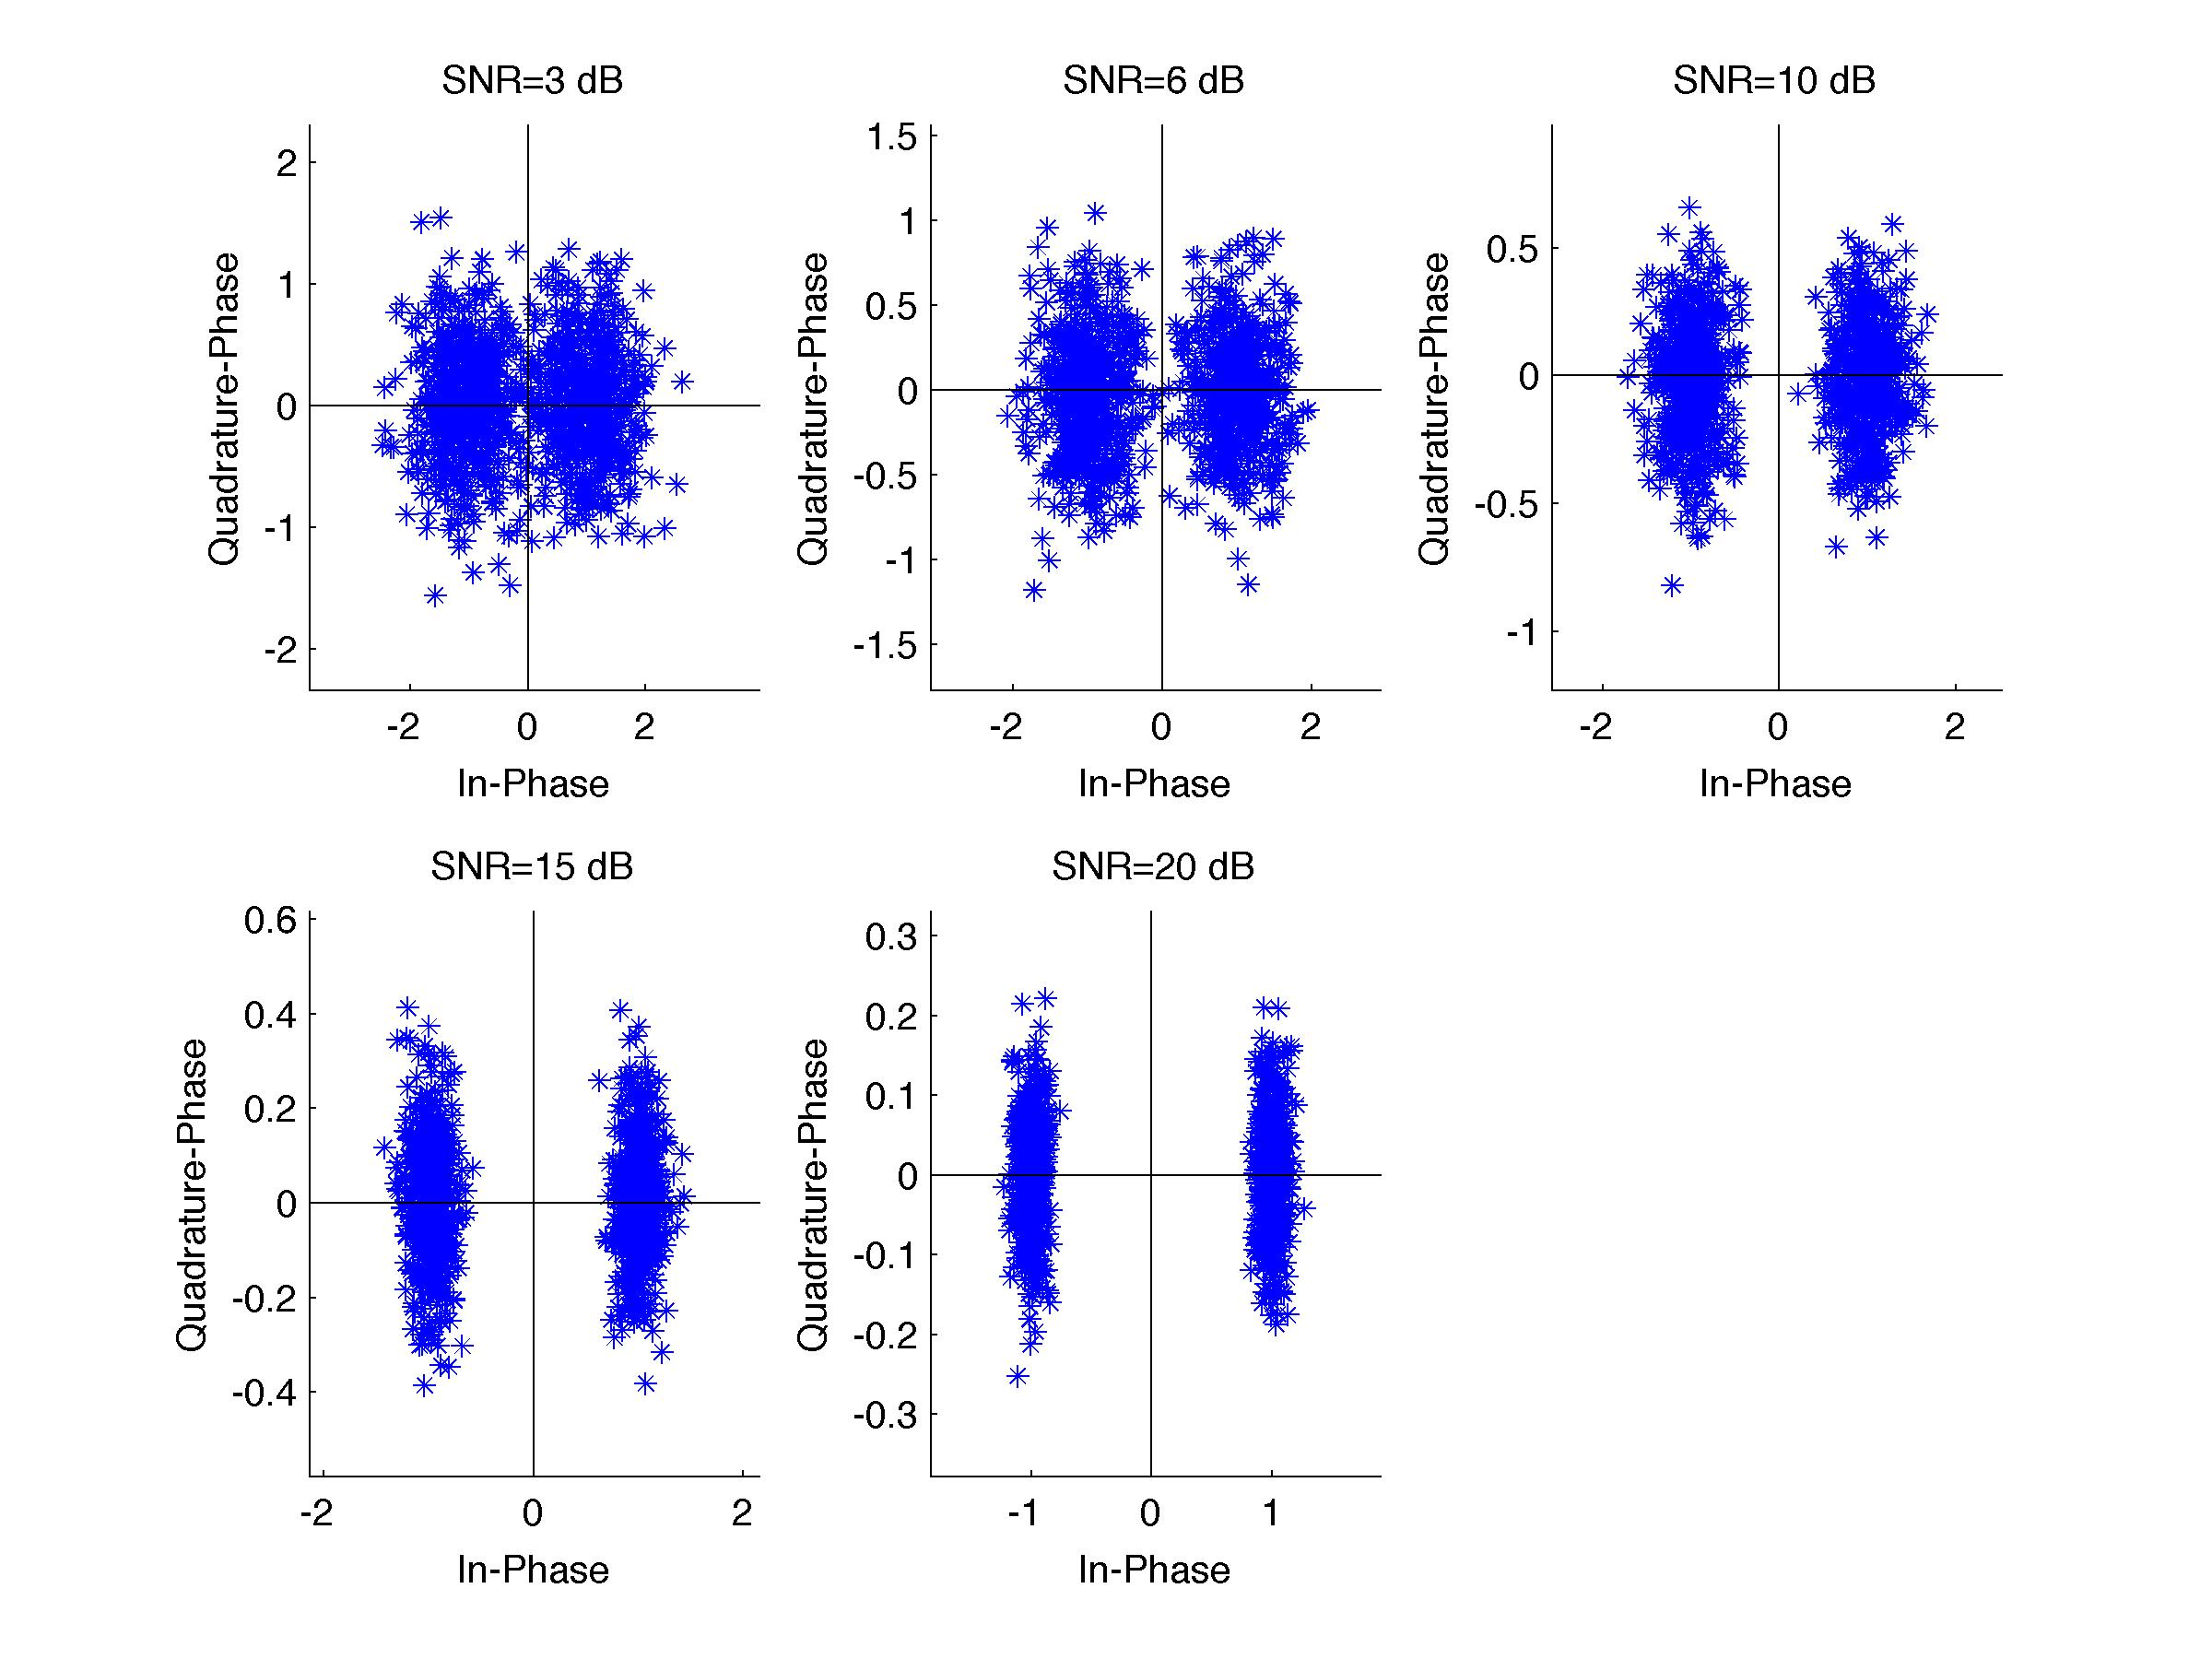
\includegraphics[width=1.3\textwidth]{bpConstfo3.jpg}
\caption{The BPSK constellation plots for different levels of SNR at a frequency offset of 1 Hz}
\end{figure}

\begin{figure}[H]
\centering
\hspace*{-2cm}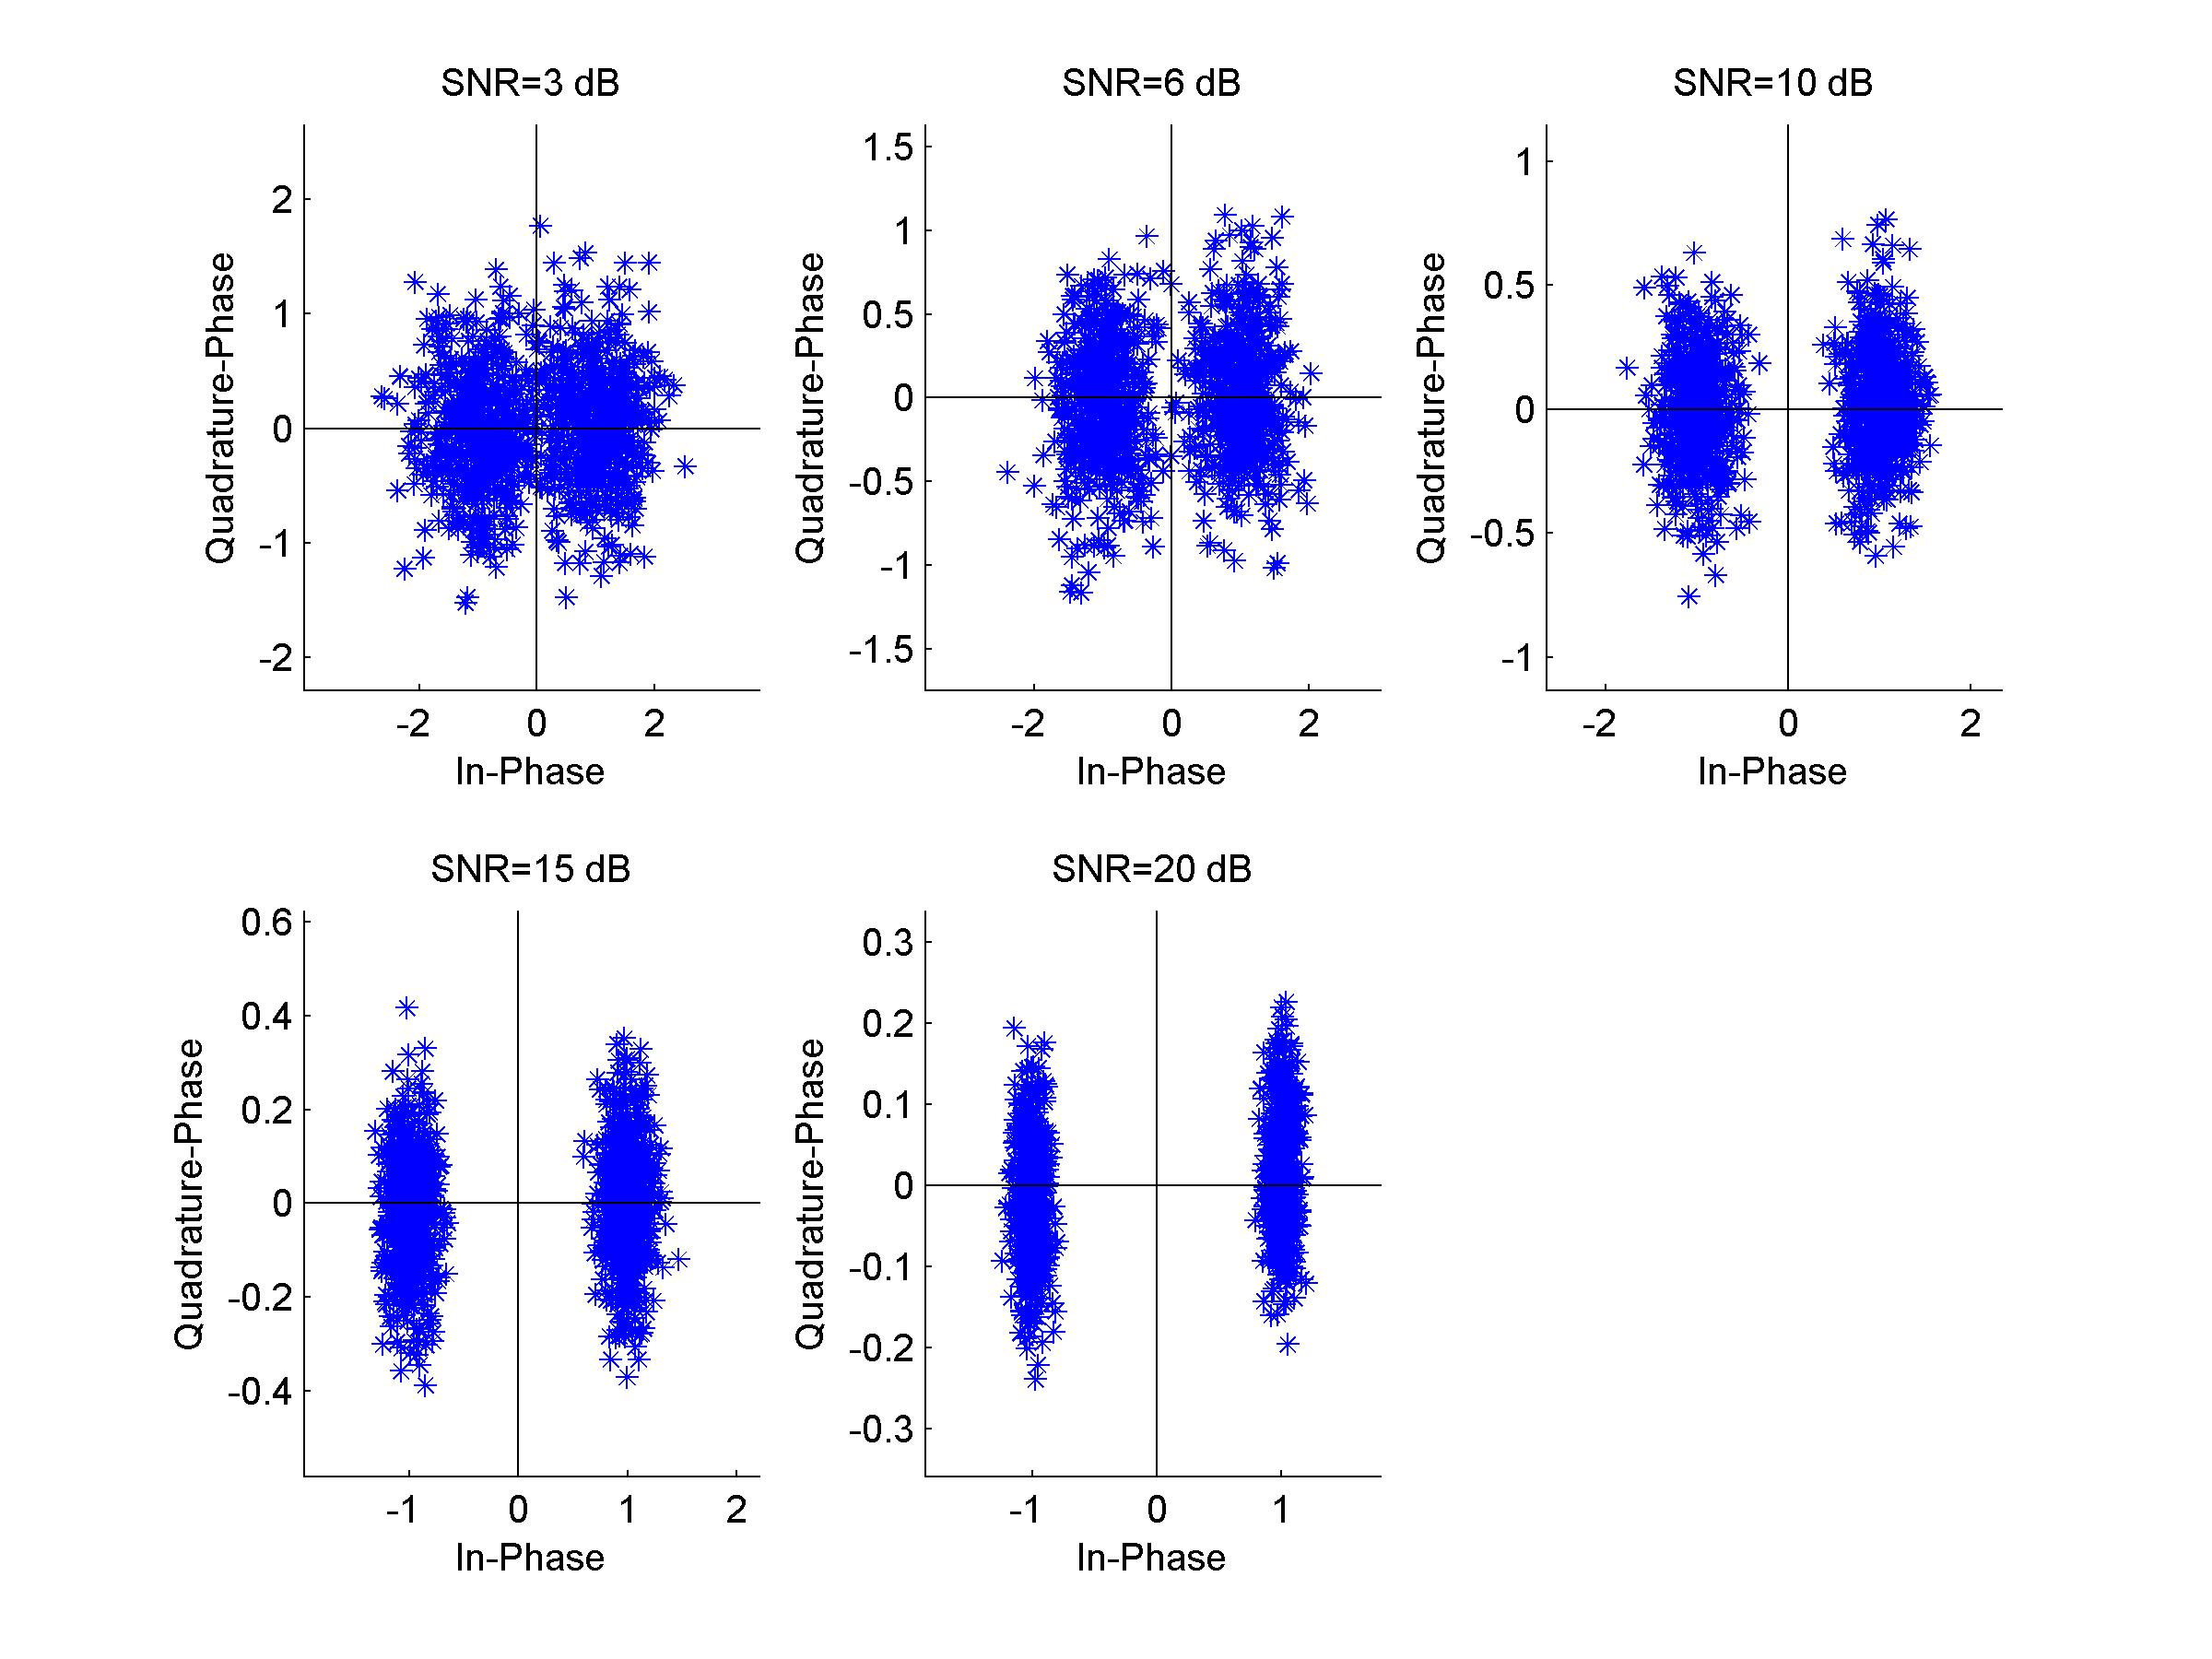
\includegraphics[width=1.3\textwidth]{bpConstfo4.jpg}
\caption{The BPSK constellation plots for different levels of SNR at a frequency offset of 10 Hz}
\end{figure}

\subsubsection{QPSK with Frequency Offset}
\begin{figure}[H]
\centering
\hspace*{-2cm}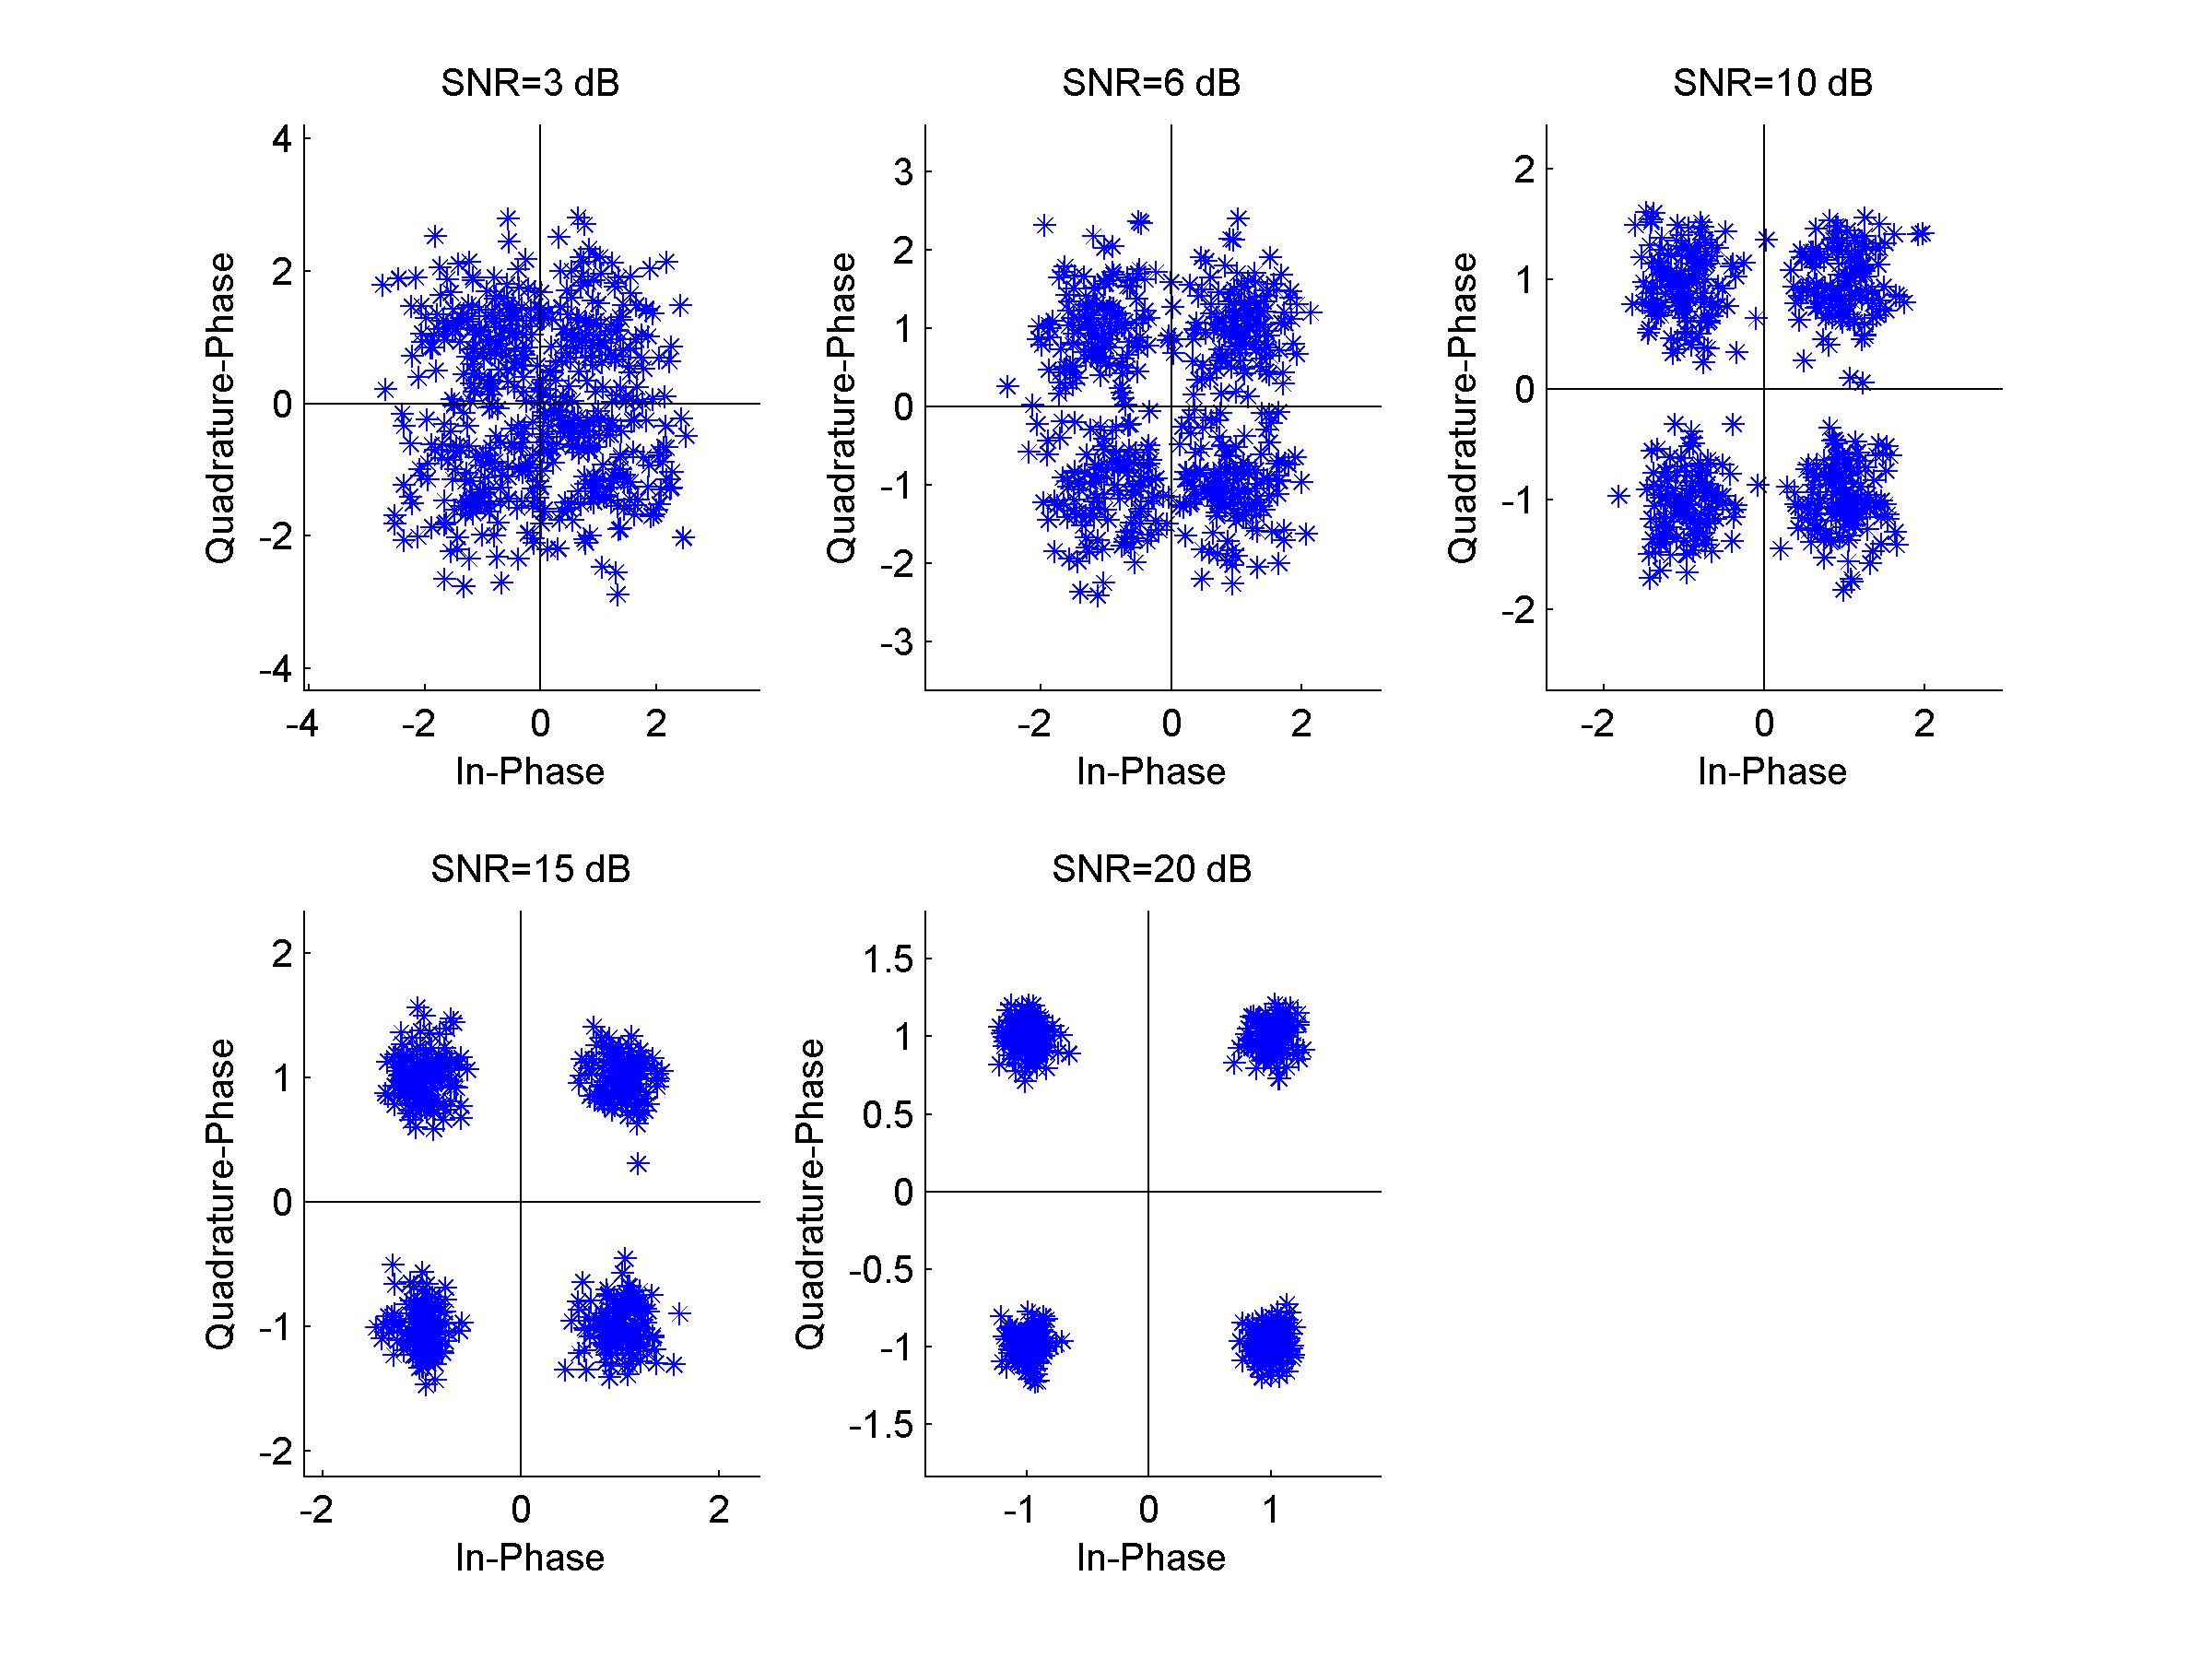
\includegraphics[width=1.3\textwidth]{qpConstfo1.jpg}
\caption{The QPSK constellation plots for different levels of SNR at a frequency offset of 0.01 Hz}
\end{figure}

\begin{figure}[H]
\centering
\hspace*{-2cm}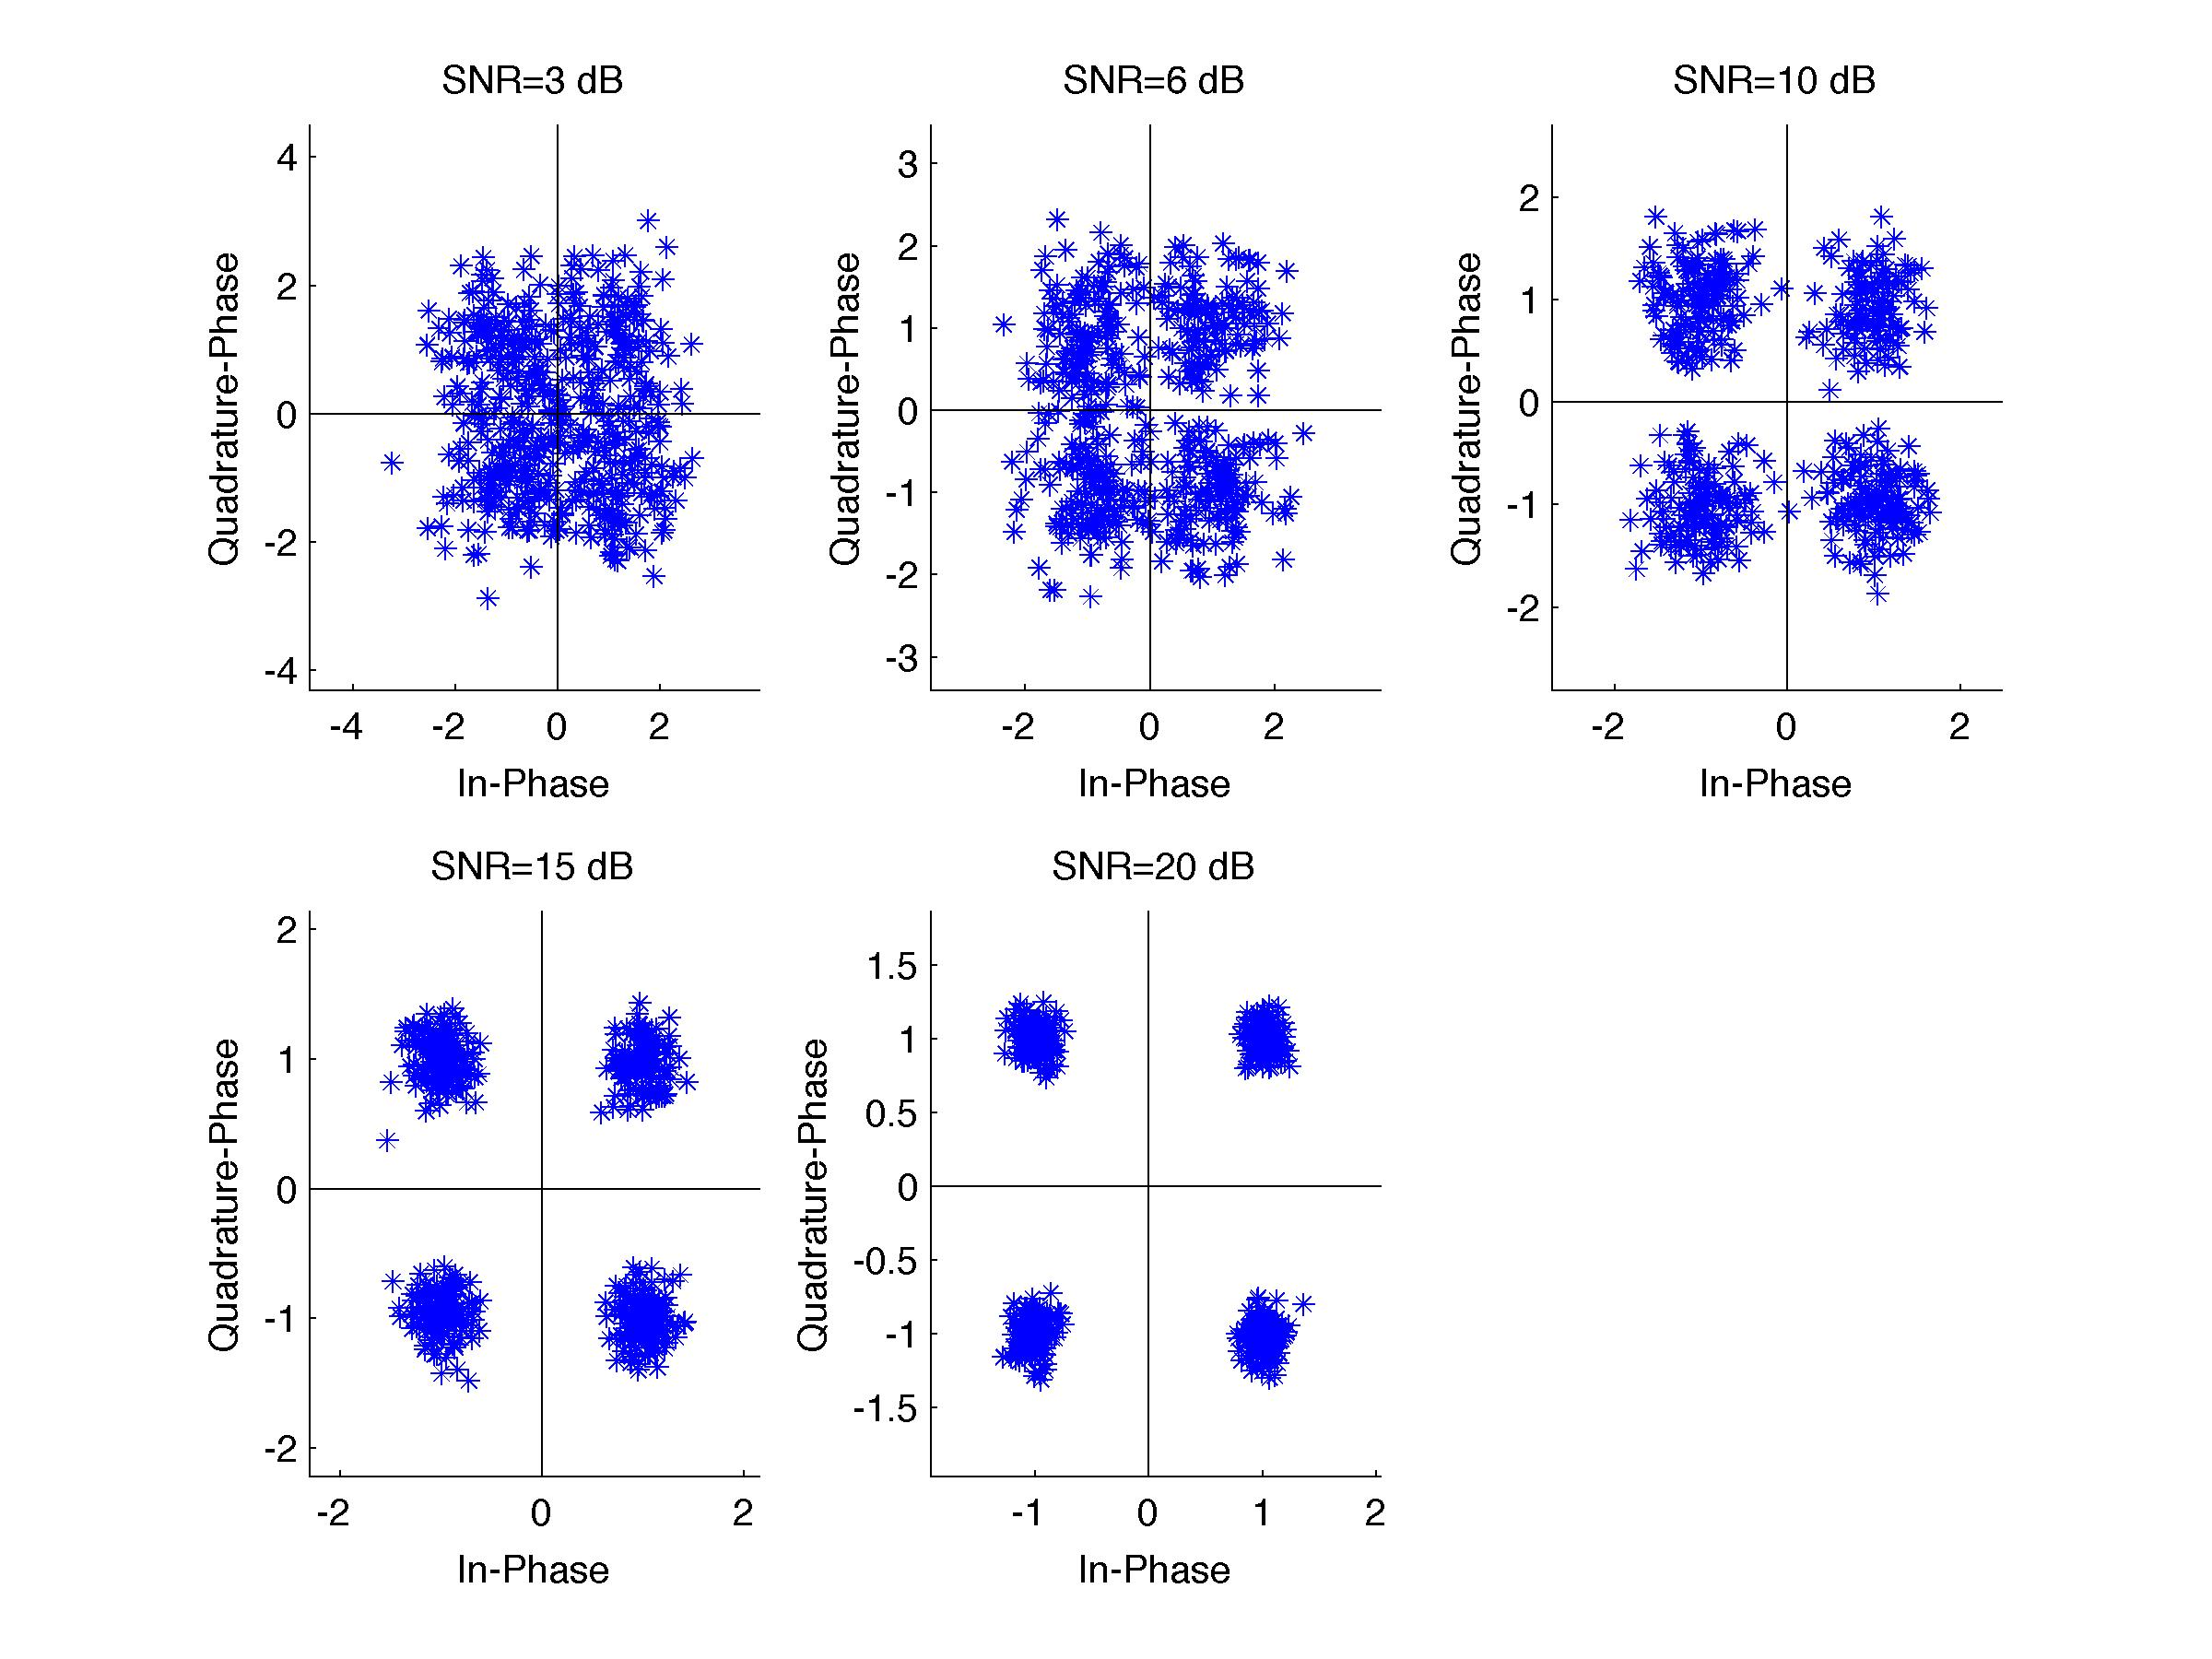
\includegraphics[width=1.3\textwidth]{qpConstfo2.jpg}
\caption{The QPSK constellation plots for different levels of SNR at a frequency offset of 0.1 Hz}
\end{figure}

\begin{figure}[H]
\centering
\hspace*{-2cm}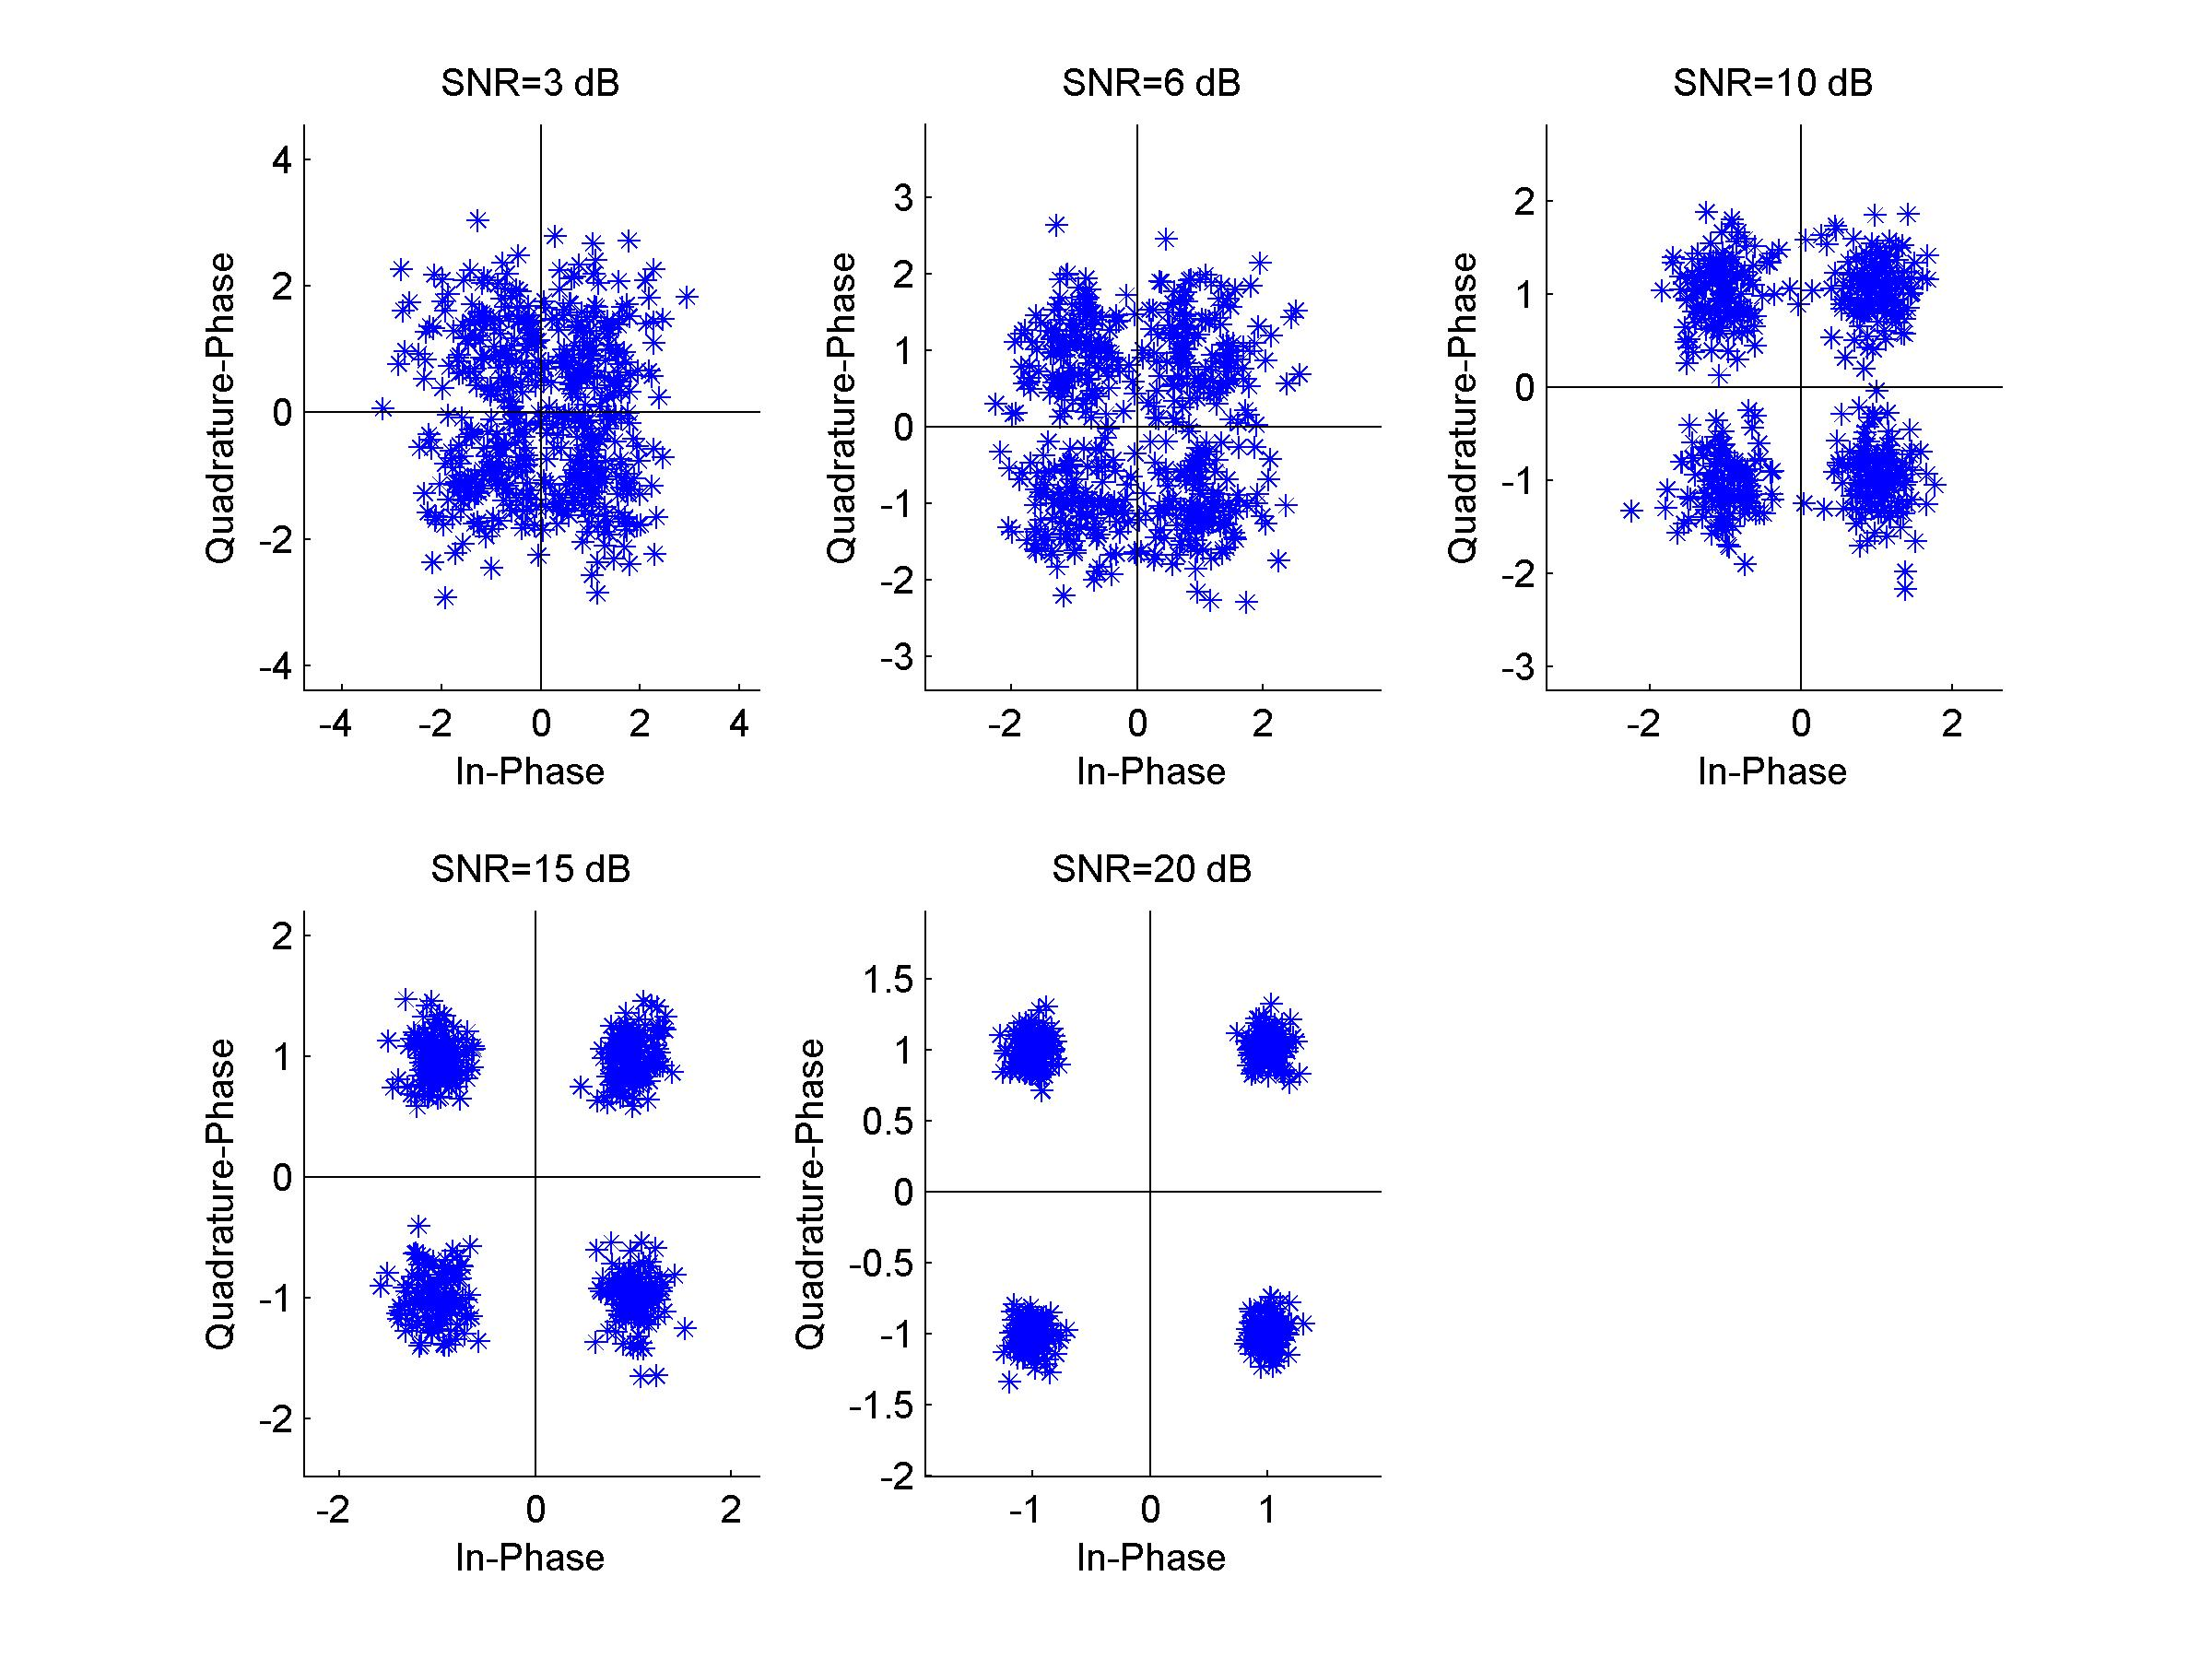
\includegraphics[width=1.3\textwidth]{qpConstfo3.jpg}
\caption{The QPSK constellation plots for different levels of SNR at a frequency offset of 1 Hz}
\end{figure}

\begin{figure}[H]
\centering
\hspace*{-2cm}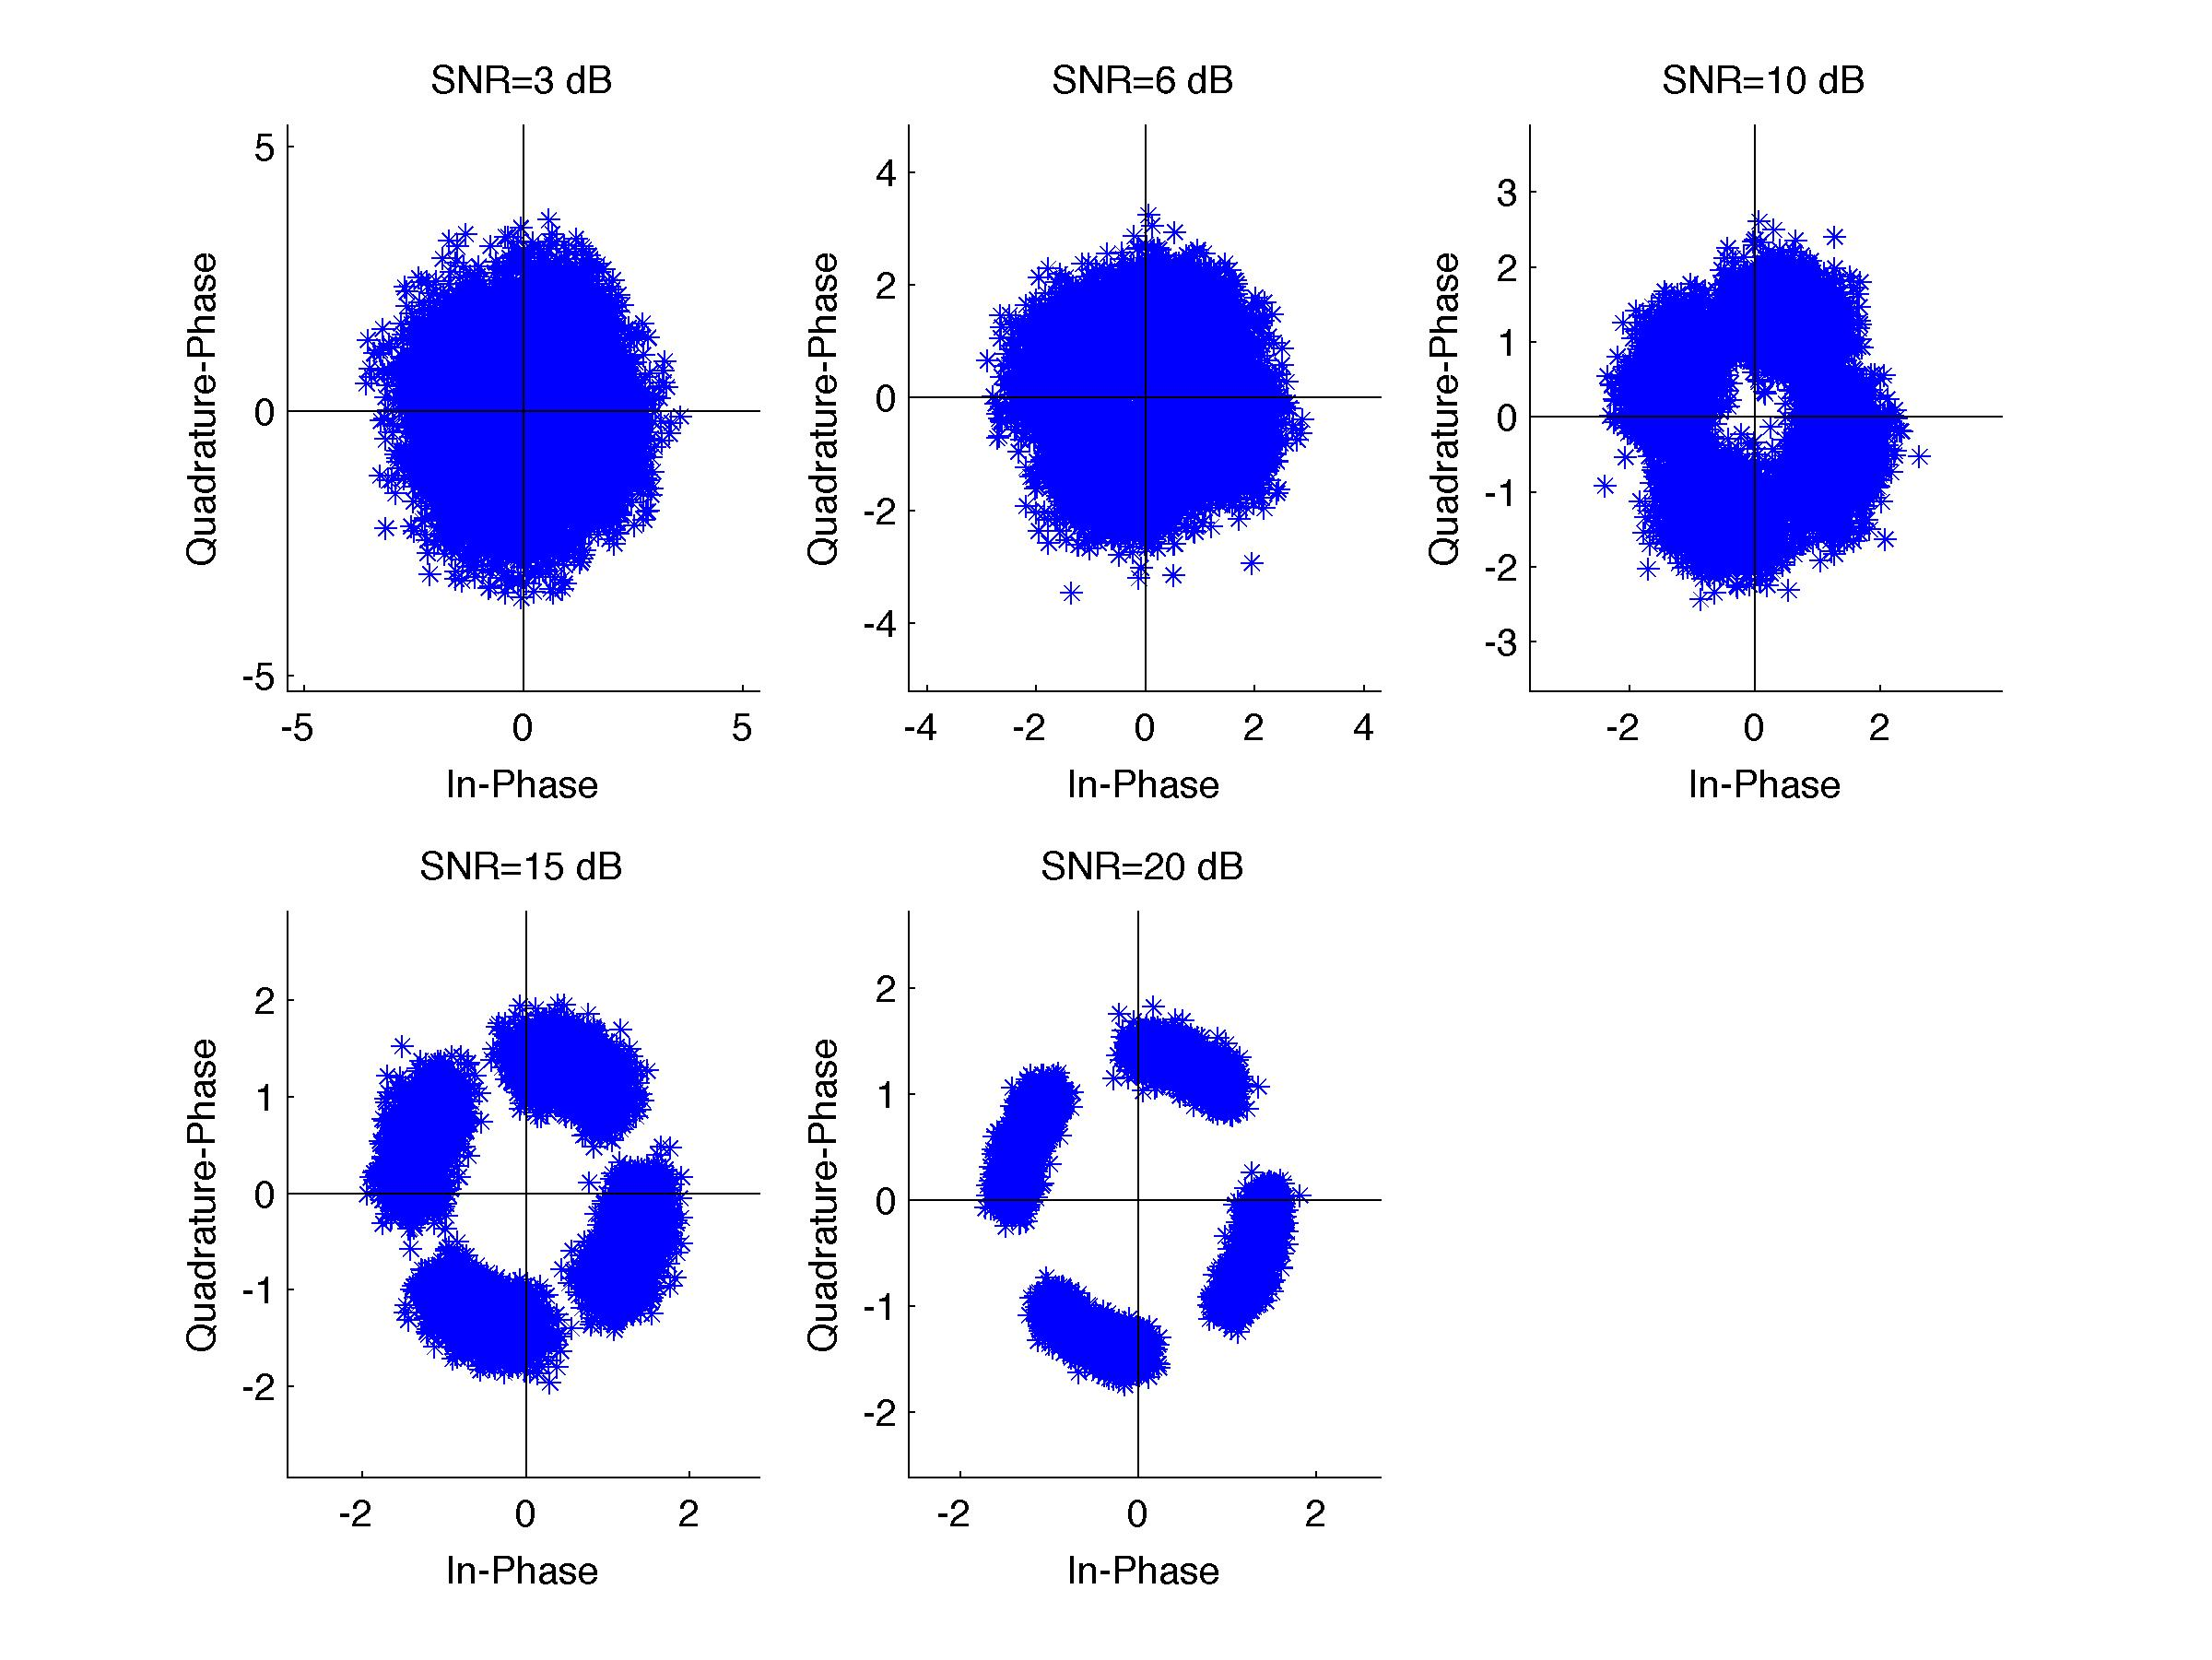
\includegraphics[width=1.3\textwidth]{qpConstfo4.jpg}
\caption{The QPSK constellation plots for different levels of SNR at a frequency offset of 10 Hz}
\end{figure}


\newpage
\section{Conclusion}
\label{sec:conc}
This phase of the project showed effects of carrier phase and frequency offsets.  This occurs in real systems when coherency is not maintained.  The models showed that bit error rates were not rendered unusable by small errors.  As phase got to $\frac{\pi}{4}$ off, the constellations became the same as for proper $\frac{\pi}{4}$-QPSK [Section~\ref{sec:qam16_phaseConst}].  Similarly, the frequency errors did not ruin the transmissions [\ref{sec:results_fo}].  

\appendix
\newpage
\bibliographystyle{plain}
\bibliography{step2}
\newpage
%% the \\ insures the section title is centered below the phrase: Appendix B
%\section{Project Assignment}
%\label{app:assign}
%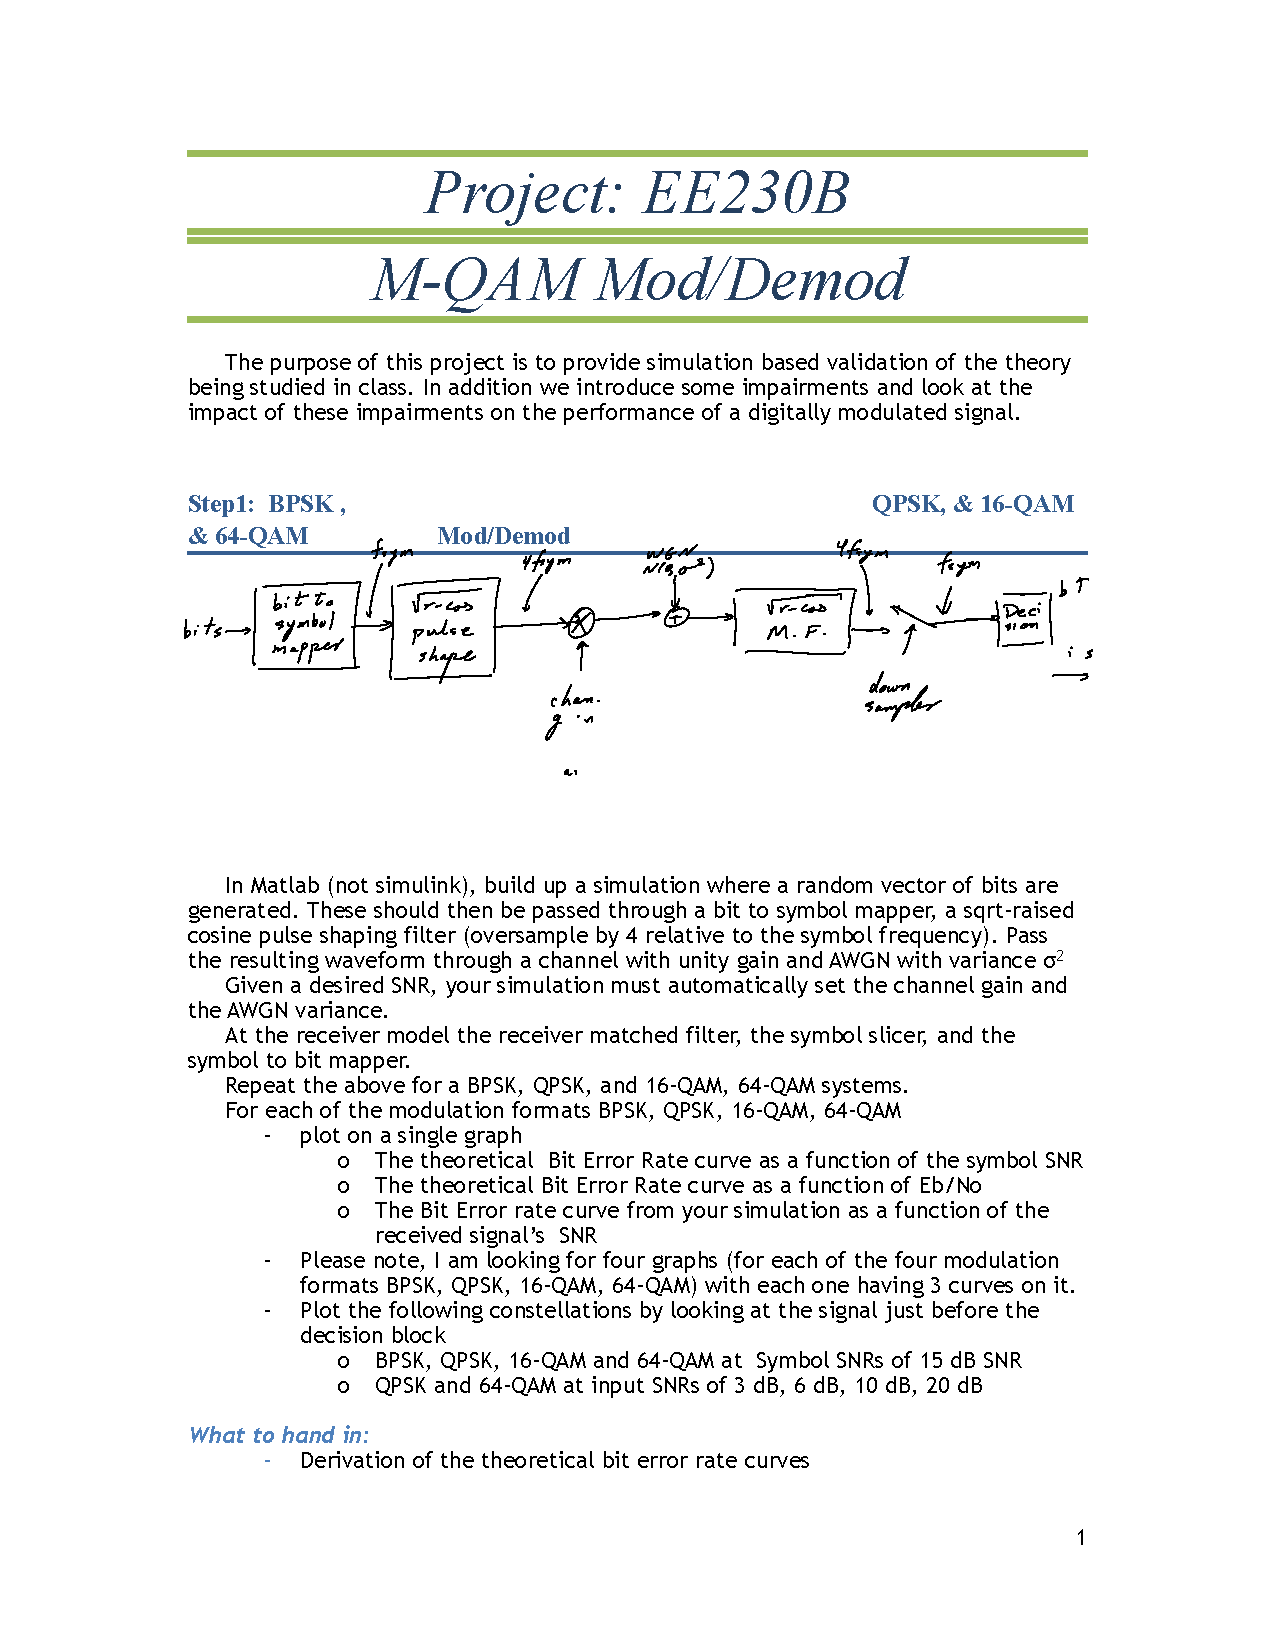
\includepdf[pages={1-5}]{project_overview.pdf}
%\cleardoublepage
%\newpage


\section{Random Bit Sequence Generator}
\label{app:random_bit_generator}
\lstinputlisting{random_bit_generator.m}

\section{Bit to Symbol Mappers}
\label{app:bittosym}
\subsection{BPSK Modulation }
\label{app:bpsk_mod}
% To convert program (e.g. C++ Fortran, Matlab, LaTeX) listings to a
% form easily includable in a LaTeX document
%
% type lgrind -s to see options
% lgrind -llatex -i sample-paper.tex > sampleinputtex
% creates a file sampleinput.tex which can then be included into this
% document simply by uncommenting the next line
%\lgrindfile{testinput.tex}

\lstinputlisting{bpsk_mod.m}

\subsection{QPSK Modulation}
\label{app:qpsk_mod}
\lstinputlisting{qpsk_mod.m}

\subsection{16-QAM Modulation}
\label{app:qam_16_mod}

\lstinputlisting{QAM_16_mod.m}

\subsection{64-QAM Modulation }
\label{app:qam_64_mod}
\lstinputlisting{QAM_64_mod.m}

\newpage
\section{Square Root Raised Cosine Filter}
\label{app:sqrt_raised_cosine}
\lstinputlisting{sqrt_raised_cosine.m}


\section{Up Sampler}
\label{app:impulse_train}
\lstinputlisting{impulse_train.m}

\section{Additive Gaussian White Noise Channel}
\label{app:awgn_channel}
\lstinputlisting{awgn_complex_channel.m}

\newpage
\section{Sampler}
\label{app:sampler}
\lstinputlisting{sampler.m}


\section{Decision Blocks}
\label{app:dblocks}
\subsection{BPSK Demodulation}
\label{app:bpsk_demod}
\lstinputlisting{bpsk_demod.m}

\newpage
\subsection{QPSK Demodulation}
\label{app:qpsk_demod}
\lstinputlisting{qpsk_demod.m}

\subsection{16-QAM Demodulation}
\label{app:qam_16_demod}
\lstinputlisting{QAM_16_demod.m}

\newpage
\subsection{64-QAM Demodulation}
\label{app:qam_64_demod}
\lstinputlisting{QAM_64_demod.m}

\newpage
\section{Offsets}
\label{app:offsets}
\subsection{Carrier Phase Offset}
\label{app:phase_offset}
\lstinputlisting{phase_offset.m}

\newpage
\subsection{Carrier Frequency Offset}
\label{app:freq_offset}
\lstinputlisting{freq_offset.m}


\end{document}